\documentclass[12pt,a4paper,oneside,openright]{report} % uses the default cls report, no separate cls file:  ,twoside

\usepackage{xpatch} % an extention to etoobox for redefining commands 
\makeatletter % the redefined macro name contains @

%\usepackage{url}
\usepackage{thesis} % uses style modifications, titlepage from thesis.sty 

\usepackage{xurl} % handle line breaks in long URL strings gracefully

\usepackage[T2A,T1]{fontenc} % the last specified encoding defines it
\usepackage[utf8]{inputenc}
\usepackage[russian,UKenglish]{babel}

% Use single quotes around titles:
\usepackage{csquotes}

\usepackage{natbib}
\usepackage{har2nat}

\renewcommand{\harvardurl}{Available at: \url}
%\newcommand*{\newunitpunct}{\addcomma\addspace} % comma as separator in bibliography, not full stop

\bibliographystyle{wolves}  % agsm gives comma after year in References, NO comma intext, in before Proceedings; all 7 harvard styles are wrong, editing apsr. See: https://tex.stackexchange.com/questions/134258/harvard-style-bibliography-with-biblatex-almost-but-not-quite/134264#134264

\usepackage{verbatim}

\usepackage{todonotes} % Used for inserting comments inline or in the margins.

\usepackage{amsmath} % allows align environments for equations

\usepackage[a4paper,inner=23mm,outer=25mm,top=15mm,bottom=30mm,includehead]{geometry} % recto and verso pages
\setlength{\headheight}{15pt}% to address the warning:\headheight is too small (12.0pt): Make it at least 14.49998pt

%%% Add any other packages you need to use here.
% import the listings package that defines a style for syntax highlighting depending on the language
\usepackage{float}
\usepackage{makecell}
\usepackage{tabularx} 

\usepackage{rotating}  % wrap your figure in \begin{sidewaysfigure} .. \end{sidewaysfigure}

\usepackage{caption}
\captionsetup[figure]{font=small}
\captionsetup[table]{font=small}
\usepackage{multirow}
\usepackage[inline,shortlabels]{enumitem} % \begin{enumerate}[(a)] % (a), (b), (c), ...
% the first par moved the multiline content of items, the second indents the bolded item 
\setlist[description]{leftmargin=3em, labelindent=\parindent} 

\usepackage{soulutf8}
\usepackage{xcolor}  % [dvipsnames]

\usepackage{color, colortbl}
%\definecolor{ForestGreen}{RGB}{0,150,100}
\definecolor{Dandelion}{RGB}{255,127,0}
\definecolor{cadmiumgreen}{rgb}{0.0, 0.42, 0.24}
%\definecolor{chromeyellow}{rgb}{1.0, 0.65, 0.0}

\usepackage{multicol}

%
% This file defines a style for code listings, including syntax
% highlighting.
%

\usepackage{xcolor}
\definecolor{tenPercentGrey}{gray}{0.9}

% COLORS (Tango) Mostly by Philip Bunge
% http://pbunge.crimson.ch/
\definecolor{White}{gray}{0.9}
\definecolor{Black}{gray}{0.0}
\definecolor{LightButter}{rgb}{0.98,0.91,0.31}
\definecolor{LightOrange}{rgb}{0.98,0.68,0.24}
\definecolor{LightChocolate}{rgb}{0.91,0.72,0.43}
\definecolor{LightChameleon}{rgb}{0.54,0.88,0.20}
\definecolor{LightSkyBlue}{rgb}{0.45,0.62,0.81}
\definecolor{LightPlum}{rgb}{0.68,0.50,0.66}
\definecolor{LightScarletRed}{rgb}{0.93,0.16,0.16}
\definecolor{Butter}{rgb}{0.93,0.86,0.25}
\definecolor{Orange}{rgb}{0.96,0.47,0.00}
\definecolor{Chocolate}{rgb}{0.75,0.49,0.07}
\definecolor{Chameleon}{rgb}{0.45,0.82,0.09}
\definecolor{SkyBlue}{rgb}{0.20,0.39,0.64}
\definecolor{Plum}{rgb}{0.46,0.31,0.48}
\definecolor{ScarletRed}{rgb}{0.80,0.00,0.00}
\definecolor{DarkButter}{rgb}{0.77,0.62,0.00}
\definecolor{DarkOrange}{rgb}{0.80,0.36,0.00}
\definecolor{DarkChocolate}{rgb}{0.56,0.35,0.01}
\definecolor{DarkChameleon}{rgb}{0.30,0.60,0.02}
\definecolor{DarkSkyBlue}{rgb}{0.12,0.29,0.53}
\definecolor{DarkPlum}{rgb}{0.36,0.21,0.40}
\definecolor{DarkScarletRed}{rgb}{0.64,0.00,0.00}
\definecolor{Aluminium1}{rgb}{0.93,0.93,0.92}
\definecolor{Aluminium2}{rgb}{0.82,0.84,0.81}
\definecolor{Aluminium3}{rgb}{0.73,0.74,0.71}
\definecolor{Aluminium4}{rgb}{0.53,0.54,0.52}
\definecolor{Aluminium5}{rgb}{0.33,0.34,0.32}
\definecolor{Aluminium6}{rgb}{0.18,0.20,0.21}

%%% LISTINGS

\usepackage{listings}

\lstset{
  backgroundcolor=\color{tenPercentGrey}, %
  basicstyle=\color{Black}\ttfamily{}, %
  keywordstyle=[1]\color{DarkSkyBlue}, %
  keywordstyle=[2]\color{DarkScarletRed}, %
  keywordstyle=[3]\bfseries{}, %
  keywordstyle=[4]\color{DarkPlum}, %
  keywordstyle=[5]\color{SkyBlue}, %
  commentstyle=\color{Aluminium4}, %
  stringstyle=\color{Chocolate}, %
  identifierstyle=\color{Black}, %
  emphstyle=\color{Black}, %
  numbers=left, %
  stepnumber=1, % 
  frame=tb, %
  captionpos=b, %
  lineskip=\smallskipamount{}, %
  aboveskip=\bigskipamount{}, %
  belowskip=\medskipamount{}, %
  commentstyle=\itshape\small{}, %
  tabsize=2, %
  breaklines=false, %
  rulecolor=\color{Black!30}, %
  showspaces=false, %
  showstringspaces=false, %
  showtabs=false, %
} % chktex 6

\lstloadlanguages{Python,[LaTeX]TeX}

%%% this provides color to hyperref
\setuphyperref{}{}

\usepackage{booktabs}  % See: http://texdoc.net/texmf-dist/doc/latex/booktabs/booktabs.pdf

% a package to build a list of abbreviations and to keep track of them
\usepackage{longtable}
\usepackage{array,multirow,graphicx} 
% change font to Times New Romans
%\usepackage{mathptmx} % - sets \rmdefault to 'ptm', i.e. times
%\renewcommand{\familydefault}{ptm} % using \rmdefault here doesn't work
%\usepackage{libertine}
% Helvetica
%\renewcommand{\sfdefault}{phv}
%\renewcommand{\familydefault}{\sfdefault}

%  If you want to suppress the hyperlink for a particular instance, use the starred form \gls*{svm} 
% supress fullstop and page index
% run in terminal to add new terms to the pre-compiled file: makeglossaries phd
\usepackage[acronym,automake,nopostdot,nonumberlist]{glossaries}
\makeglossaries % create makeindex files

\usepackage{smartdiagram} % for a flowchart at p.135
\usepackage{tikz}

\newcommand{\specialcell}[2][t]{%
	\begin{tabular}[#1]{@{}l@{}}#2\end{tabular}}

% typesetting examples with chapterwise numbering
\usepackage{linguex}  % https://texdoc.org/serve/linguex-doc.pdf/0

% We want that the label to an example has also the section number
\renewcommand{\Exarabic}{\thesection.\arabic} 

% We want to reset the ExNo counter at each section
\usepackage{chngcntr}
\counterwithin{ExNo}{section}
\usepackage{cleveref}
\crefname{ExNo}{}{examples}

% We want cross references of the form "1.1.1"
\creflabelformat{ExNo}{#2#1#3}


%Numbered environment with double counter-within
\newcounter{example}
\counterwithin*{example}{section} % asterisk/star avoids redefining theexample (second number in 1.2) in each section
\newenvironment{examples}[1][mytitle]{\refstepcounter{example}\par\medskip
	\noindent \textbf{Example~\thesection.\theexample. #1}\par \rmfamily}{\medskip}

\usepackage[titletoc]{appendix} % this import is needed to add Appendix to TOC


\def\boxit#1{%
	\smash{\color{red}\fboxrule=1pt\relax\fboxsep=2pt\relax%
		\llap{\rlap{\fbox{\vphantom{0}\makebox[#1]{}}}~}}\ignorespaces
}

\makeatletter\@addtoreset{section}{part}\makeatother%


\begin{document}

%%% \thesistitle ends the preamble.
% Thesis title, author and name.
\thesistitle{Translationese indicators \\for human translation quality estimation \\(based on English-to-Russian translation \\of mass-media texts)} {Maria Kunilovskaya} {May 2023}
% Human translation quality: linguistic description and automatic estimation
% Human translation quality: translationese and distributional embeddings approaches

% Thesis abstract.
\addcontentsline{toc}{chapter}{Abstract}

% Experiments with document-level quality labels confirmed that lower-ranking translations bear signs of passive translational behaviour associated with transfer of ST patterns and failure to introduce items, specific to the TL.

\chapter*{Abstract}
% motivation and gap
Human translation quality estimation is a relatively new and challenging area of research, because human translation quality is notoriously more subtle and subjective than machine translation, which attracts much more attention and effort of the research community. At the same time, human translation is routinely assessed by education and certification institutions, as well as at translation competitions. Do the quality labels and scores generated from real-life quality judgments align well with objective properties of translations? This thesis puts this question to a test using machine learning methods.

% hypothesis and rationale
% Goal: Compare automatic prediction results (learnability) for several quality labels/scores on a number of representations
Conceptually, this research is built around a hypothesis that linguistic properties characteristic of translations, as a specific form of communication, can correlate with translation quality. This assumption is often made in translation studies but has never been put to a rigorous empirical test. Exploring translationese features in a quality estimation task can help identify quality-related trends in translational behaviour and provide data-driven insights into professionalism to improve training. Using translationese for quality estimation fits well with the concept of quality in translation studies, because it is essentially a document-level property. Linguistically-motivated translationese features are also more interpretable than popular distributed representations and can explain linguistic differences between quality categories in human translation.

% features/reps
We investigated (i) an extended set of Universal Dependencies-based morphosyntactic features as well as two lexical feature sets capturing (ii) collocational properties of translations, and (iii) ratios of vocabulary items in various frequency bands along with entropy scores from n-gram models. To compare the performance of our feature sets in translationese classifications and in quality estimation tasks against other representations, the experiments were also run on \textit{tf-idf} features, \textit{QuEst++} features and on contextualised embeddings from a range of pre-trained language models, including the state-of-the-art multilingual solution for machine translation quality estimation. Our major focus was on document-level prediction, however, where the labels and features allowed, the experiments were extended to the sentence level.

% design: data, labels, methods
The corpus used in this research includes English-to-Russian parallel subcorpora of student and professional translations of mass-media texts, and a register-comparable corpus of non-translations in the target language. Quality labels for various subsets of student translations come from a number of real-life settings: translation competitions, graded student translations, error annotations and direct assessment. We overview approaches to benchmarking quality in translation and provide a detailed description of our own annotation experiments. 

% results and interpretation
Of the three proposed translationese feature sets, morphosyntactic features, returned the best results on all tasks. In many settings they were secondary only to contextualised embeddings. At the same time, performance on various representations was contingent on the type of quality captured by quality labels/scores.
Using the outcomes of machine learning experiments and feature analysis, we established that translationese properties of translations were not equality reflected by various labels and scores. For example, professionalism was much less related to translationese than expected. 
Labels from document-level holistic assessment demonstrated maximum support for our hypothesis: lower-ranking translations clearly exhibited more translationese. They bore more traces of mechanical translational behaviours associated with following source language patterns whenever possible, which led to the inflated frequencies of analytical passives, modal predicates, verbal forms, especially copula verbs and verbs in the finite form. As expected, lower-ranking translations were more repetitive and had longer, more complex sentences. Higher-ranking translations were indicative of greater skill in recognising and counteracting translationese tendencies. For document-level holistic labels as an approach to capture quality, translationese indicators might provide a valuable contribution to an effective quality estimation pipeline. 

However, error-based scores, and especially scores from sentence-level direct assessment, proved to be much less correlated by translationese and fluency issues, in general. This was confirmed by relatively low regression results across all representations that had access only to the target language side of the dataset, by feature analysis and by correlation between error-based scores and scores from direct assessment.

\singlespace{\tableofcontents}

% Acknowledgements
\thispagestyle{empty}
\vspace*{\stretch{1}}
\begin{flushright}
    \emph{To Andrey Kutuzov}
\end{flushright}
\vspace*{\stretch{3}}
\addcontentsline{toc}{chapter}{Acknowledgements}

\chapter*{Acknowledgements}

%not only the giants whose shoulders provided the proverbial support for this work, by also people who were beside me throughout this endeavour, who supported and encouraged me

First and foremost, I would like to acknowledge Prof. Ruslan Mitkov, the heed of the Research Group in Computational Linguistics at the University of Wolverhampton, who is very good at creating opportunities for other people. For me, this PhD programme was a wonderful chance to convert a hobby into a full-time occupation and to considerably progress and achieve personal goals that I had little hope to achieve otherwise. It applies to many other academic activities apart from the PhD research: supporting the Master's programme, working for the Journal of Natural Language Engineering, organising conferences. 

I want to express my belated appreciation of the diligence and consistency of my first-year supervisory team: Prof. Constantin Orasan and Dr. Sara Moze. They were key to installing me on the right track and mood for this research. 

Special thanks go to Andrey Kutuzov for all the inspiration, and mocking, and practical help; for countless discussions and genuine curiosity. Above all, I see him as a person who initiated my interest in empirical linguistics in the first place.

I am grateful to Serge Sharoff for the human warmth and kindness, for starting conversations, for his keen interest in my developments and for the shared linguistic passions. He is one of the those people who would not cringe at the perspective of talking about research.

Big thanks to Ekaterina Lapshiniva-Koltunski, my co-author in many publications, for the shared interest in the translationese studies and not begrudging the time to discuss it. suggesting useful and relevant reading, for   

I should mention Vasilisa Grosheva, my eldest daughter for tolerance when being shamelessly used as a sounding board to fly my research ideas. It meant a lot to me and in the long run helped to shape this thesis. And also, for silently taking over the household chores.
% I am guilting of having her read parts of this thesis as another pair of eyes, along with taking care of younger siblings and other animals.  
% kids for always lending an ear for my lengthy talks; overused as a sounding board.

I am grateful to Evgeniy Medvedev, my brother, who had an unwavering faith in me and offered useful support (including computational) and encouragement throughout the years of my studentship. This support meant a lot to me. 

Although the COVID pandemic interfered midway, I was happy to share the Wolverhampton office and many lunches with my colleagues: Alistair Plum, Shiva Taslimipoor, Omid Rohanian, Rocío Caro, Tharindu Ranasinghe. These people moulded my attitudes and experiences in this research field and supplied their bits that in the end joined as a jigsaw (or not). There is a special person in the RGCL office who always made me feel welcome and valued: April Harper, the most considerate and empathetic person I met. I think she is that key player, a constant in the RGCL team who glues together the pieces and smoothens the processes.

Finally, I want to embrace all the people in the NLP and the computational linguistics communities who do not see reviewing as a useless and formal chore, but believe that they are contributing to the progress in the field. Everybody knows that there is nothing more rewarding for an author than a knowledgeable, understanding and well-wishing critic who can suggest better options and ask the right questions. 

%We would like to acknowledge Donald Craig at Memorial University,
%Newfoundland who published the meta-thesis on which this template is
%based. You can find Donald's work on his web site, here:
%\url{http://www.cs.mun.ca/~donald/metathesis/}.



% Automatically generated tables.

\addcontentsline{toc}{chapter}{List of Tables}
\singlespace{\listoftables}

\addcontentsline{toc}{chapter}{List of Figures}
\singlespace{\listoffigures}

%\addcontentsline{toc}{chapter}{List of Code Listings}
\singlespace{\lstlistoflistings}

% to make glossary appear, run in terminal: texstudio/phd_text$ makeglossaries phd
\addcontentsline{toc}{chapter}{Abbreviations}
\glsaddall
% abbreviations:
\newacronym{HTQE}{HTQE}{human translation quality estimation}
\newacronym{MTQE}{MTQE}{machine translation quality estimation}
\newacronym{QE}{QE}{quality estimation}
\newacronym{MT}{MT}{machine translation}
\newacronym{TS}{TS}{Translation Studies}
\newacronym{ATA}{ATA}{American Translation Association}
\newacronym{HT}{HT}{human translation}
\newacronym{SL}{SL}{source language}
\newacronym{TL}{TL}{target language}
\newacronym{ST}{ST}{source text}
\newacronym{TT}{TT}{target text}
\newacronym{ML}{ML}{machine learning}
\newacronym{LM}{LM}{language model}
\newacronym{PoS}{PoS}{Parts of speech}
\newacronym{RusLTC}{RusLTC}{Russian Learner Translator Corpus}
\newacronym{RNC}{RNC}{Russian National Corpus}
\newacronym{BNC}{BNC}{British National Corpus}
\newacronym{MQM}{MQM}{Multidimensional Quality Metrics}
\newacronym{DQF}{DQF}{TAUS Dynamic Quality Framework}
\newacronym{WMT}{WMT}{Conference on Machine Translation}
\newacronym{STS}{STS}{Semantic Textual Similarity}
\newacronym{PCA}{PCA}{Principal Component Analysis}
\newacronym{SVM}{SVM}{Support Vector Machines}
\newacronym{SVR}{SVR}{Support Vector Regressor}
\newacronym{LTC}{LTC}{learner translator corpora}
\newacronym{NLP}{NLP}{Natural Language Processing}
\newacronym{TTR}{TTR}{type-to-token ratio}
\newacronym{BiLSTM}{BiLSTM}{bi-directional Long Short-Term Memory}
\newacronym{ANOVA}{ANOVA}{analysis of vaiance}
\newacronym{RFE}{RFE}{recursive feature elimination}
\newacronym{RFECV}{RFECV}{Cross-validated RFE}
\newacronym{LDA}{LDA}{Linear Discriminant Analysis}
\newacronym{MFW}{MFW}{most frequent words}
\newacronym{TQA}{TQA}{Translation Quality Assessment}
\newacronym{TQE}{TQE}{Translation Quality Estimation}
\newacronym{UD}{UD}{Universal Dependencies}
\newacronym{MWE}{MWE}{multi-word expressions}
\newacronym{DM}{DM}{discourse markers}
\newacronym{PMI}{PMI}{pointwise mutual information}
\newacronym{MI}{MI}{mutual information}
\newacronym{NPMI}{NPMI}{normalised pointwise mutual information}
\newacronym{OOV}{OOV}{out-of-vocabulary}
\newacronym{L1}{L1}{mother tongue}
\newacronym{FTD}{FTD}{Functional Text Dimensions}
\newacronym{TMX}{TMX}{Translation Memory eXchange}
\newacronym{XML}{XML}{Extensible Markup Language}
\newacronym{EWT}{EWT}{English Web Treebank}
\newacronym{BLEU}{BLEU}{Bilingual Evaluation Understudy}
\newacronym{METEOR}{METEOR}{Metric for Evaluation of Translation with Explicit ORdering}
\newacronym{HTER}{HTER}{Human Translation Error Rate}  % aka Human-targeted Translation Error Rate
\newacronym{TER}{TER}{Translation Error Rate}
\newacronym{DA}{DA}{Direct Assessment}
\newacronym{NMT}{NMT}{Neural Machine Translation}
\newacronym{SMT}{SMT}{Statistical Machine Translation}
\newacronym{PE}{PE}{post-editing}
\newacronym{CAT}{CAT}{Computer-Assisted Translation}
\newacronym{MAE}{MAE}{Mean Absolute Error}
\newacronym{RMSE}{RMSE}{Root Mean Square Error}
\newacronym{ROC}{ROC}{receiver operating characteristic}
\newacronym{AUC}{AUC}{area under (ROC) curve}
\newacronym{STD}{STD}{standard deviation}
\newacronym{BERT}{BERT}{Bidirectional Encoder Representations from Transformers}
\newacronym{XLM-R}{XLM-R}{XLM-RoBERTa}
\newacronym{RNN}{RNN}{recurrent neural networks}
\newacronym{CNN}{CNN}{convolutional neural networks}
\newacronym{IRA}{IRA}{Inter-rater agreement}
\newacronym{IRR}{IRR}{Inter-rater reliability}
\newacronym{API}{API}{application programming interface}
\newacronym{ReLU}{ReLU}{Rectified Linear Units}
\newacronym{tf-idf}{tf-idf}{term frequency--inverse document frequency}
\newacronym{SOTA}{SOTA}{state-of-the-art}
% Do not separate these files with spaces.
\printglossary[type=\acronymtype,title=Abbreviations]
 % add all abbreviations to abbr.tex, call then in-text as \gls{} or \gls*{}

\pagenumbering{arabic}\setcounter{page}{1}
\pagestyle{fancy} % see \usepackage{fancyhdr} in thesis.sty
% Your own thesis chapters go here.
\chapter{\label{cha:intro}Introduction}
%\addcontentsline{toc}{chapter}{Introduction}
% New title: Student translation quality: (norm-based) lingustic description and automatic estimation
% Learner translations: lingustic description and automatic quality estimation
% Human translation quality: translationese and distributional embeddings approaches
%
%\todo[inline]{(1) introduce a convention to refer to comparable originally authored texts in Russian as non-translation, a term first used in this meaning by~\cite{Chesterman2004}\\ (2) mention that all examples unless specifically marked come from our corpus, esp. RusLTC part of it}

\section{\label{sec:motivation}Motivation and Background}
% this section contextualises the problem and gives the rationale behind the research design
% aboutness and personal motivation
%My experience in translator education of many years led me to believe that translations, and student translations in particular, share specific features that make them recognisable as such. 
%Year after year, I annotated and commented the same suboptimal translation solutions. Their repetitiveness suggested that student translations can have automatically recognisable properties, which can be used to predict their quality. 

This thesis presents a comprehensive study of the relations between translationese and translation quality as captured by various assessment methods. 
%This thesis explores persistent properties of human translations in English-to-Russian language pair, testing the long-known and theoretically expected tendencies in translational behaviour as well as inferring new ones in a bottom-up manner. % new ones: I did not expect these to be among 28 shared translationese indicators amod/attrib, nnargs, wdlength, ccomp, pverbals, compar, fixed
It explores claims about translationese in English-to-Russian translation made in practical translation textbooks and arising from personal experience, and extends the existing scope of knowledge about the properties of translated language, making these properties even more visible to a professional eye. It often requires to know where to look to actually see. Raising awareness of the peculiarities of translated language can be useful in translator training, helping students to avoid typical pitfalls and recognise the cognitive constraints of the translation process. Importantly, this thesis investigates the extent to which translationese properties are taken into account in judgments about translation quality.
The originality and novelty of this study consists in testing the link between translationese and quality in a ML setup for the first time. 

% introduce the area of study
\paragraph{Area of study and rationale} 
%This research is set at the interface of empirical translation studies, corpus linguistics, computational linguistics and \gls{NLP}. Findings about linguistic properties of translated texts are based on experimental results obtained using machine learning techniques to predict quality labels and to reveal aspects of linguistic form that are objectively correlated with the available human judgments on translation quality. 

We draw from several research fields at various stages of this project trying to bridge the gap between theoretical translation studies and computational linguistics using supervised \gls{ML} methodologies. They can be roughly outlined as follows:
\begin{itemize}\compresslist{}
	\item translation quality related theories, including assessment approaches;
	\item empirical and computational translation studies focused on translationese research and studies on professionalism in translation;
	\item corpus linguistics focused on student translation and (register-)comparable corpora;
	\item machine translation quality research including human assessment methods and quality benchmarks;
	\item machine learning approaches to solve translationese-related and quality estimation tasks.
\end{itemize}

% contextualise the research, outline the current situation, introduce key terms
The specificity of translations in comparison with their sources and non-translated texts in the same target language register was acknowledged in literary criticism long ago. For example,~\citet{Berman1985} formulated 12 deforming tendencies in literary translation, including rationalisation (making text more coherent), ennoblement (more elegant style), destruction of underlying networks of signification, etc. However, it was not before Baker's seminal work~\cite{Baker1993} that translations and its linguistic properties became an object of study in their own right. After almost three decades of research, one of the central concepts in translation studies, \textit{translationese}, can be broadly defined as statistical deviations of translations from the expected target language norm, i.e. from language manifested in comparable originally-authored texts in the \gls{TL}. The body of research exploring peculiar regularities of translated language can be referred to as \textit{translationese studies}. 

From early works on, translationese was viewed as a strictly descriptive, non-evaluative term reflecting the nature of translation~\cite{Gellerstam1986, Baker1993}. It was established that all translations are inevitably different from comparable originally-authored texts. It does not mean that translated texts are written to a lower professional standard than comparable non-translations~\cite{Sutter2017}. Instead, they form their own language subsystem and can be approached as a language variety.

% why do this research?
% why the proposed approach is feasible
% hypothesis
At the same time, the amount and type of translationese observed in translations can be indicative of translation quality. For translation scholars and educators, professionalism in translation is often associated with the ability to identify translation problems and find the more acceptable solution for them~\cite{Pym2003}, i.e., most importantly, to be able to recognise and counteract the natural gravitational pull of the \gls{SL} which triggers literal renditions.

The association between the amount of translationese and translation quality was either assumed or demonstrated in a number of publications, such as~\citet{Scarpa2006, Rabadan2009, Sutter2017} as well as in~\citet{Loock2013, Loock2016}~\cite[as quoted by][]{Sutter2017}. For example,~\citet{Scarpa2006} found that simplification correlated with lower-scoring translations and explicitation correlated with higher quality scores. \citet{Sutter2017} interpreted the distance between individual student translations and comparable professional texts in scatter plots as indicative of lower quality. They also found statistical differences between student and professional translations in a univariate analysis on a number of language-independent easily-extractable features in English-to-French translation of fiction and in French-to-Dutch news. Our own early univariate exploration of student translations indicated that they were more distant from the reference corpus than professional translations on a number of linguistically-motivated features~\cite{Kunilovskaya2018profiles}.

% establish a niche, identify the gap
Despite \textit{translationese studies} is an established research direction in the empirical translation studies, the applicability of translationese features to \gls{HTQE} remains unclear. It is especially surprising, given that translationese-based approach was used in a much more dynamic and technologically advanced area of \gls{MTQE}~\cite{Aharoni2015} and in the machine translation detection task~\cite{Carter2012}. In particular, \citet{Aharoni2015} showed that the higher the translationese classification accuracy (i.e. the better machine translations were distinguished from non-translations), the lower the expected translation quality. \citet{Aranberri2020} also found translationese predictive of~\gls{MT} quality. Interestingly, \citet{Rubino2016} used surprisal and distortion measures derived from delexicalised language models, which they refer to as quality estimation indicators, to discriminate between novice and professional translations.
Nonetheless, we are not aware of any empirical studies that explore the suggested feasibility of a translationese-based human translation quality model. %, except our own previous work~\cite{Kunilovskaya2019qua, Kunilovskaya2020vars}.

\paragraph{Hypothesis} Thus, this research is designed to test a hypothesis that translationese indicators could be predictive of human translation quality. This hypothesis will be confirmed if we find that lower-ranking translations exhibit stronger translationese tendencies than their higher-ranking counterparts, and if a ML algorithm built to predict quality labels/scores returns a reasonably high performance compared to alternative representations.  

Generally, this research contributes to a fairly new research area of automatic prediction of human translation quality. The term \gls{HTQE} seems to have first appeared in a PhD thesis by~\citet{Yuan2018} and a subsequent publication by the same author~\cite{Yuan2020}. In their work, the concept of quality estimation for~\gls*{MT} is adopted to predict English-to-Chinese human translation quality. 
The alternative automatic approach to MT quality (quality evaluation) measures deviations from a MT candidate and human reference translations. It is hardly applicable to human translation, even theoretically, due to a wide range of legitimate variation in linguistic expression that translators can resort to. In human translation, it seems unfair to penalise renditions because they deviate from a pre-selected good translation.
In another research on HTQE, known to us, \citet{Zhou2019} formulated the task of predicting human translation quality as an unsupervised graph matching problem. They employ cross-lingual word embeddings to represent sources and targets, and measured the distance between respective vectors, reporting Spearman 0.529 for their Japanese-to-English data. 

%\todo[inline]{We did the same in a supervised setting on self-trained cross-lingual projection (MUSE) achieving the best result on binary quality labels of macro F1-score = 63.0, the current result on our focused representation is 61.40, with the chance level of 51.63. Shall I report that?}
Other attempts to develop automatic approach to measure human translation quality were not formulated as a ML task, but present corpus-based studies and observations. \citet{Sutter2017} report results of a multifactorial corpus analysis backed with \gls{PCA}-based visualisation to give a translation teacher a method to `objectify formative quality assessment' (p.25). They perform monolingual comparison, presenting student translations against the backdrop of comparable professional translations and non-translations as two possible TL norms, and reducing the concept of human translation quality to its acceptability aspect, i.e. to the TL quality. 

% disadvantages of the proposed approach
\paragraph{Anticipated issues and challenges} We envisage a few theoretical and practical challenges that should be kept in mind. This paragraph discusses caveats that limit the scope of this research and possible contingency measures to curb their effects on the outcomes. 
One limitation of a translationese-based approach to translation quality estimation is that it reflects only one of translation quality aspects, namely, fluency (also referred to as acceptability/readability). It does not have access of the semantic relation between source and target texts, known as the accuracy/adequacy aspect of translation. Nonetheless, as it is shown in Sections~\ref{sec:feats4qua} and~\ref{ssec:bin}, there are good reasons to believe that 
\begin{itemize}\compresslist{}
	\item translationese-related fluency might have a large impact on human perception (`It does not sound right' reaction),
	\item fluency and accuracy might be difficult distinguish in an annotation task, 
	\item fluency and accuracy might correlate to a great extent -- it is difficult to imagine a human translation produced in good faith that is very fluent but inaccurate; inaccuracies usually render translated text less readable and coherent than expected and are rarely seamless,
	\item differences between student and professional translations are mostly related to the fluency aspect of translation quality.
\end{itemize}

Frequency-based translationese features are not immune to sparsity. At sentence-level, where the observations are short, many features can have zero values. Therefore, the proposed features, especially from the morphosyntactic feature set, are better suited for document-level experiments.
%provided that the documents are of suitable lengths (typically, of at least 450 words; the studies that use chunking usually limit their text fragments by 2000 tokens).

Assessing translations on the basis of translationese indicators, requires carefully selected external resources that would represent the expected standard, i.e. either comparable professional translations, or reference texts, or both. It is not uncommon to collect and maintain such resources in both educational~\citep{Bowker2001} and industrial settings (translation memories and \gls*{TL} reference corpora)~\citep{Massey2019}, but such resources can be less available in other circumstances. 
Constructing a comparable corpus of non-translations to represent \gls*{TL} textual fit~\citep{Chesterman2004} is one of the challenges in this project. Register of the source and translational conventions associated with it are known to be one of the major factors shaping linguistic properties of translations~\cite{Lapshinova2017}. A preliminary step in this research was to design an approach to select a subset of non-translations from a large TL corpus that would be functionally-comparable to the English source texts in the parallel subcorpora~\cite{Kunilovskaya2019crossling}.

By design, this research is focused on shining-through form of translationese. Some researchers express reservations whether SL-induced translationese can explain all specificity of translations. They name other factors that might be at work, including translators' awareness of their sociocultural roles and positions, i.e. translation norms~\cite{Laviosa2008, Delaere2012}, extralinguistic conditions of the translation situation such as time constrains and perceived responsibility, rather than lack of professionalism and inadequate language use. It is necessary to control for some of these other factors in the experiment design by selecting register-homogeneous translations produced under similar communicative and translation conditions by many subjects of known professional status.

%application, practical relevance
% low-risk taking examination scoring and autonomous learning feedback
\paragraph{Practical relevance} This thesis primarily contributes to the understanding of translationese and its relation to quality judgments. Our results can be used as a module in a \gls{HTQE} tool to estimate translation quality with regard to the amount of translationese manifested it a translated document. There is a number of potential use cases for \gls*{HTQE}, primarily in education, certification and quality control.

Probably the largest sphere where there is a wide need to score human translations is translator education and language learning scenarios. Translation programmes of various standing (university degrees in translation, vocational training courses or advanced professional development programmes) as well as practical translation courses included in the foreign language education programmes routinely grade students' written submissions. Some form of summative assessment is indispensable in test and exam settings. However, although institutional grading manuals can be very detailed, translation quality assessment often proceeds ``according to the lordly, but completely unexplained, whimsy of `It doesn't sound right.''', a much quoted and accurate description offered by~\citet[p. 142]{Fawcett1981}. An automated approach can make this process more objective and systematic, devoid of personal preferences and expectations, more uniform in terms of rigour, and immune to the known negative effects common for all human evaluation, including lapses of concentration and the order of translations to be graded~\cite{MinacoriVibert2010}.    

A reliable automation of the scoring process can help to better monitor translation students' progress and provide qualitative feedback on their work more often. It is true that getting regular formative human feedback on their course work between the tests would be more useful, but, given the class sizes and the enormous effort required to assess translations manually, it is unavailable in many translation programmes.
Automatic feedback can also contribute to self-evaluation and independent learning. 

Apart from qualification exams in the training environments, many countries have certification requirements that facilitate the access to professional jobs. Certification usually includes a translation task, which is scored by several trained evaluators. In the context of the \gls{ATA}, there is a points-based threshold (more than 46) after which the error annotation can be abandoned because the translation is obviously below the expected quality standard\wlvfootnote{see the instructions at \url{www.atanet.org/certification/Framework_2017.pdf}}. An automatic scoring algorithm can be used as a preliminary filter to identify the submissions that can be desk-rejected for being significantly below the standard. A similar functionality can be useful for filtering out very poor submissions to translation contests to help a human jury focus on, for example, the top 30\% of the participants to identify the winners. 

In the industrial contexts, an automatic scoring tool for human translations can be applied on both the language service provider side for internal quality control purposes or on the customer side for ensuring the quality of a translation obtained from a translator or a translation agency, possibly as an extension of Translation Quality Assurance procedures, if they are available. It can be especially useful if a translation user does not possess a bilingual competence and does not want to involve a third party for a linguistic expertise. A similar need for a quick and cheap evaluation of translation quality arises when several human translations of the same sample are available and the customer is seeking to detect the best of them. 

\section{\label{sec:task}Research Aim and Objectives}
% overarching purpose of a research project
% two main aspects: linguistic(!) features and four labels: comparison to other representations and extension to doc- and sent-level is implied
This thesis sets out to explore the performance of translationese indicators inspired by contrastive linguistics and translation studies in the task of predicting a range of human translation quality judgments.

To achieve this overarching purpose, we define a number of research objectives:
\begin{enumerate}\compresslist{}
	\item Develop a set of translationese indicators motivated by previous findings in translationese studies and contrastive analysis for English-to-Russian language pair (mass-media register).
	\item Test the proposed feature sets in a translation detection task (translationese classification) on two competence-based varieties (student and professional translations). This objective includes:
	\begin{enumerate}[(a)]\compresslist{}
		\item building a motivated comparable corpus of non-translations, the second class in the translationese-diagnostic binary classification (translations vs. non-translations); 
		\item comparing the performance of proposed feature sets to each other and to alternative representations, including multilingual/cross-lingual embeddings;
		\item identifying and describing strong translationese indicators.
	\end{enumerate}
	\item Collect various types of human quality judgments. This involves a number of preliminary steps:
	\begin{enumerate}[(a)]
		\item explore the approaches to produce quality labels in human and machine translation applicable to our data;
		\item build a parallel corpus of professional translations and generate a reasonably diverse subset of student translation from an existing \gls{LTC} to represent experience-based categories as a proxy for quality;
		\item produce quality labels from existing \gls{RusLTC} `grade' attribute and continuous document- and sentence-level scores from existing error annotation.
		\item set up a direct assessment annotation experiment and produce respective document- and sentence-level scores.
	\end{enumerate} 
	\item Explore alternative approaches to text representation for document- and sentence-level quality estimation tasks. More specifically:
	\begin{enumerate}[(a)]
		\item use \textit{tf-idf} as a simple baseline,
		\item generate alternative explicit features designed for \gls*{MTQE} within QuEst++ framework, 
%		\item learn a cross-lingual distributed representation model on a register comparable corpus and use word embeddings from it, as suggested in \citet{Yuan2018,Zhou2019};
		\item apply cross-lingual sentence encoders, fine-tuned on \gls{STS} task and on DA scores in a \gls*{MTQE} task, % including \textit{TransQuest} \cite{Ranasinghe2021},
		\item generate representation from state-of-the-art general-purpose contextualised word embedding models: a dedicated Russian language model and a multilingual \textit{mdeberta3-base}.
%\todo[inline]{+ explore the possibility of combining translationese and bilingual approaches for better coverage of both fluency and accuracy aspects of quality.}
	\end{enumerate} 
	\item Compare the outcomes of classification and regression experiments, supported by feature analysis where possible, across various representations and types of quality judgments.
	% combining translationese-based approach to capturing fluency, the major problem with advanced learners translations (if the two aspects of translation quality are to be distinguished), and accuracy-oriented bilingual features and embeddings from Sentence Transformer-based models seems difficult because translationese approaches operate on the document-level, while deep-learning models are limited to short segments. Actually, the average student translation document length is within the the range that is manageable by Bert (450 tokens and 512 tokens, respectively)  
\end{enumerate}

% outline of the research design/methodology and how are we going to address the limitations
\section{\label{ssec:design}Research Design} 
This research focuses two components of a quality estimation task: types of quality labels/scores and text representations. We do not lay much emphasis on the learning algorithm and use a simple \gls{SVM} with default settings. For ML quality control, i.e. to ensure that SVM returns a reasonable performance on our tasks, we implemented a one-layer neural model.

\paragraph{Quality labels} One of the important questions that we explore in this thesis is generating translation quality benchmarks, i.e. sets of gold-standard labels/scores reflecting human judgments about translation quality that can be used as learning targets in a ML setup. 
Weak artificial intelligence, as a research and engineering domain, seeks to teach the machine to solve tasks that can be performed by humans. 
%Recent advances in neural networks demonstrate that there are fewer and fewer tasks that are exclusively human and are inaccessible to machines. 
For now, judging human translation quality is perceived as one of the tasks that is challenging for the machines. It is not entirely because it requires unstructured professional knowledge to yield to automation. It is also because translation quality is difficult to capture in a reliable way due to the notorious subjectivity of the underlying concept. This thesis compares the performance of various document representations, including translationese indicators, on labels/scores from several methods to annotate human translations for quality. These experiments can reveal dissimilarities between assessment methods with regard to the type of quality they capture. 
%However, in our experience, a professional jury in a translation contest usually agrees on the top and, especially, on bottom, translations (with possible fine-grained disagreements).   
Our experiments are run on the four types of quality categories/judgments:
\begin{enumerate}\compresslist{}
	%	\setlength{\itemsep}{0.5pt}
	\item Binary quality: coarse-grained binary quality labels, derived from holistic document-level assessment of exam translations in several Russian universities and of submissions to a number of translation competitions;
	\item Professionalism: ontological status of texts based on the meta information about translators;
	\item Scores from error annotation: aggregated measures of quality based on error statistics;
	\item Scores from direct assessment: a mean score across two annotators.
\end{enumerate}

Annotated student translations come from an existing multi-parallel \gls{LTC} which, inter alia, collects quality assessment carried out in real-life contexts (student translation competitions, graded exam translations, error annotation as part of the formative feedback). The quality judgments were produced outside of a well-controlled -- and artificial -- experimental setup.
This explains the lack of all four labels for all student translations in our research corpus. Instead, we have multiple intersecting subsets shown in Figure~\ref{fig:subsets}. We tried to acquire as much corpus data for each type of assessment as possible without compromising the integrity of the categories.
\label{pg:subsets}
\begin{figure}[h ] % htbp
	\centering
	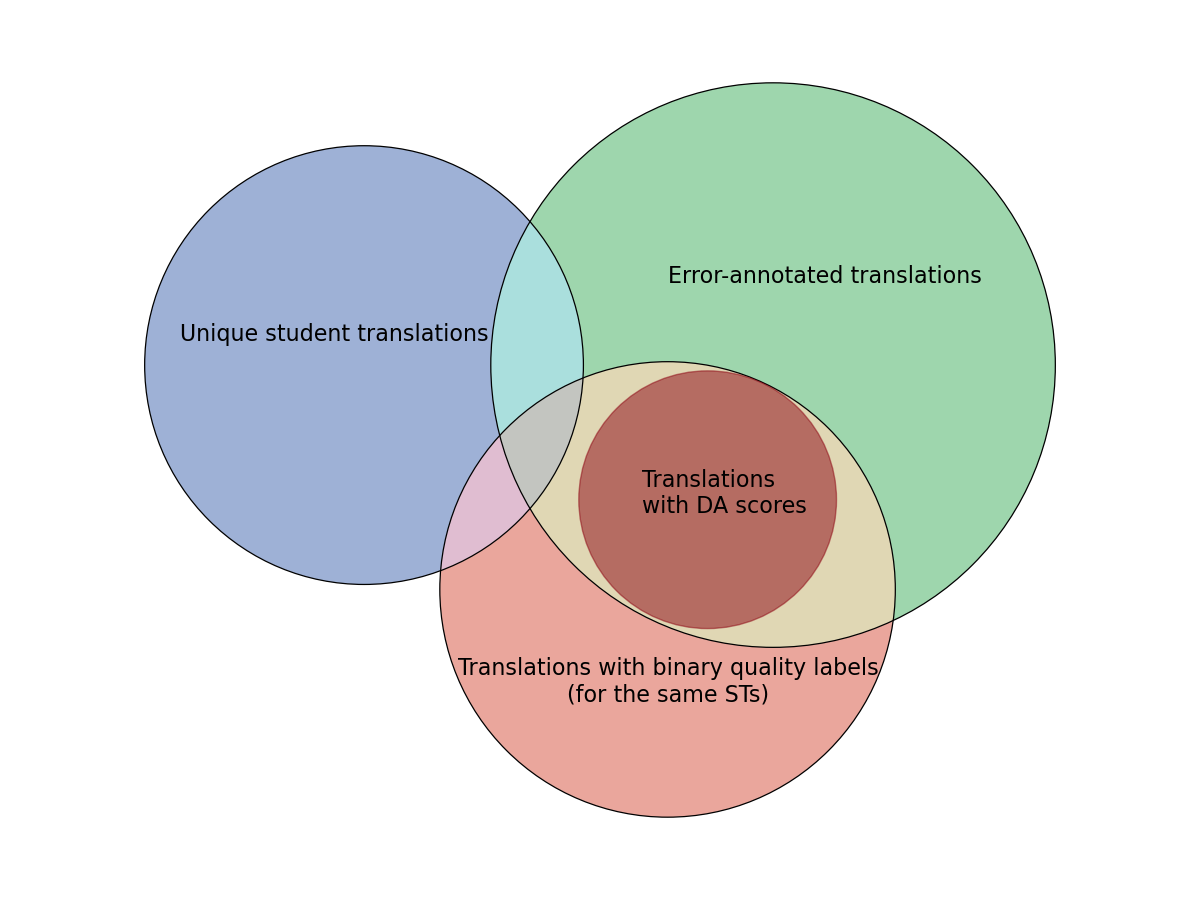
\includegraphics[scale=0.5]{figures/subsets}
	\caption{Size of student translations subsets with various types of quality judgments (number of sources, number of targets, number of aligned sentences)}
	\label{fig:subsets}
\end{figure}

%\wlvfig[0.5]{subsets}{Size of student translations subsets with various types of quality judgments (number of sources, number of targets, total number of translated sentences)}

A detailed description of how each subset was selected can be found in Section~\ref{ssec:subsets}; the annotation setups and associated reliability studies appear in Section~\ref{sec:mygold}. 

\paragraph{Features and representations} In this thesis the performance of several sets of well-established and novel language-pair specific translationese indicators is thrown into perspective of bilingual features from \textit{QuEst++}\wlvfootnote{\url{https://github.com/ghpaetzold/questplusplus}}, a translation quality estimation framework for~\gls*{MT}~\cite{Specia2015quest}, and a number of contextualised embedding models.

Traditionally, the explorations of translationese are based on manually-selected explicit features that capture a particular phenomenon represented by its normalised frequency. Probably the most popular feature set of diverse and elaborate hand-engineered features was proposed by~\citet{Volansky2012}, and later extended by~\citet{Sominsky2019}.
In the last decade, the research paradigms in translationese studies shifted from univariate statistical analyses to supervised and unsupervised \gls*{ML} methods, which take into account feature combinations. A standard practice is a bottom-up approach which includes as many features as possible and empirically establishes their effectiveness through feature selection~\cite{Evert2017, Yuan2018}. 
% which has been around since Baroni and Bernardini's~\citeyear{Baroni2005} experiments on professional English-to-Italian translations has made a comeback quite recently~\cite{Chowdhury2020,Chowdhury2021}. 
An alternative approach consists in producing sparse or dense document vectors from sequences of items in that document. Vectorisers were run on character, word or \gls{PoS} n-grams~\cite{Popescu2011,Baroni2005,Carter2012,Eetemadi2015,Rabinovich2017,Lapshinova2019}. %, because it helped with sparsity and domain differences between translations and non-translations. 
%  that retain functional words while convert other words to \gls*{PoS}
More recent studies make use of language modelling approaches (i) to measure entropy/perplexity of a model trained on non-translations and run on translations~\citep{Karakanta2019,Nikolaev2020}; or (ii) to generate static embeddings for \gls*{PoS} or semantic tags sequences in translated and non-translated corpora~\citep{Chowdhury2020,Chowdhury2021}. 

This thesis compares the performance of explicit linguistically-motivated features against representations from a number of embedding models, which are supposed to capture various properties of translations. 
The rationale behind using embeddings is that these representations might capture complex non-local syntactic and semantic information that is difficult to encode manually. Neural representations are expected to perform better than hand-engineered features, but relative ease of generating embeddings and expected superior performance come at the expense of explainability. 
%At the same time \citet{Yuan2018} results demonstrated that the power of neural models might be overestimated on the challenging task of \textit{HTQE}.    
At the moment there is no published work on translationese (or HTQE) using recent contextualised embedding models, except~\citet{Pylypenko2021}. In this thesis, we compare the performance of hand-crafted translationese indicators and document-averaged embeddings to solve the tasks of translation detection and HTQE. 

Although this research is based on human translations, we make a point of exploring theoretical and practical approaches used in \gls*{MTQE}. We are aware of the ontological differences that make these two translation varieties very dissimilar, but we hope that there can be a productive interconnection between the two closely related research areas: machine translation quality estimation and quality assessment in translation studies. 
We see it as part of our task to reveal the opportunities for mutually beneficial cooperation between machine translation and translation studies. Given our primary focus on student translations, we are mostly interested in borrowing from MT approaches to solve our task. At the same time, the increased quality of MT, especially with regard to fluency, makes the task of MTQE more demanding in terms of ability to reveal fine-grained quality distinctions.
Besides, MT paradigm can benefit from shifting to document level, which is the default setting in translation studies, and is called for in MT, especially when comparing its performance to human translators~\citep{Laubli2018,Voita2019}.

The particulars of a research design depend on the desired trade-off between interpretability, scalability and performance, among other factors. Our preferences and interests are more on the translation studies side: we use ML methods to understand the nature of translationese better and to produce interpretable automatic quality predictions, if possible. Previous research returned mixed results on language-independent generic features~\citep{Sutter2017}. Some researchers found that language-specific indicators return better results in translationese studies~\citep{Hu2021}. We are prepared to sacrifice some scalability of the approach for higher explaining power, validity and diagnostic potential. To this end, we engineer features, based on theoretical or empirical evidence from translation studies or contrastive linguistics for a given translation direction. The embeddings are used in this thesis for quality control to throw our feature-based models into perspective of the achievable for each type of labels/scores. 

\paragraph{Document- vs sentence-level} This research is focused on the document-level scenario as it is more in line with the nature of human translation. In most real-life scenarios, human translation evaluation is required at document level. 
However, it can be helpful if an algorithm could highlight segments that might require reworking or additional editing due to being inaccurate with regard to the source or due to being overtly translational at the level of expression. Besides, sentence- or segment-level predictions are more compatible with neural models. \textit{Longformer} approaches~\cite{Beltagy2020} are still in the making and are not available for Russian at the time of writing, and we had to rely on aggregation of sentence vectors via mean-pooling to obtain document representations, which might be a crude simplification.

Our experiments are framed as text classification/regression problems solved with the default linear-kernel \gls{SVM} (and a simple one-layer neural model for comparison). The classification results, including those after feature selection, are complemented with feature analysis, which traces the performance of prominent translationese indicators and their groups in quality estimation experiments.

\section{\label{sec:contributions}Main Contributions}

The main contributions of this PhD thesis are as follows: 

\begin{itemize}\compresslist{}	
	\item It proposes a theoretically-motivated feature set for translationese diagnostics in English-to-Russian translation. Its applicability to other language pairs (with adaptation) and registers has been tested in other projects, but these results are outside the scope of this thesis.
	
	\item We revealed strong translationese indicators, which were mostly associated with the \textit{shining-through} trend in translational behaviour, and demonstrated that lower-ranking translations exhibited more translationese than higher-ranking translations.  
	
	\item This study showed that morphosyntactic translationese indicators were competitive against QuEst++ features and some distributed representations, at least on document-level labels from holistic assessment. 
	
	\item It was shown that distinctions between professional and student translations were less related to translationese than expected. Professional translators might be better at recognising and counteracting some influences of the ST, but they generate other types of translationese which makes them easy to distinguish from non-translations. If anything, professional translations were more homogeneous than student translations, probably due to a more standard repertoire of translation solutions. 
	
	\item The experiments revealed dissimilarities between three quality assessment methods in terms of sensitivity to translationese and in terms of capturing document-level properties. Document-level holistic assessment was most translationese-aware, error-based scores demonstrated some alignment with translationese properties of texts and performed better at document-level. Scores from direct assessment returned better results at sentence level and were largely agnostic of translationese. 
	
	\item We released datasets for document- and sentence-level \gls{HTQE} experiments in English-to-Russian language pair with three types of quality judgments\wlvfootnote{The datasets are available from the RusLTC website: \url{www.rus-ltc.org/static/html/about.html}}. First, there is a dataset with document labels, including 360 parallel documents with good/bad labels, 738 documents with professional/student labels and 497 comparable documents originally-authored in Russian. Second, there are datasets with document- and sentence-level continuous quality scores from error annotation and from Direct Assessment experiment (553 documents/12,369 sentences with error-based scores, including 140 documents/3,224 sentences annotated in DA setup).

\end{itemize}

\section{\label{sec:papers}Publications}
%\todo[inline]{comment on the contribution of each publication to various parts of the thesis, reduce the list to only directly relevant}
Preliminary results related to the ideas developed in this thesis appeared in the following publications:
\begin{enumerate}\compresslist{}
	\item Kunilovskaya, M. and Sharoff, S. (2019) `Towards functionally similar corpus resources for translation', \textit{Proceedings of Recent Advances in Natural Language Processing}, Varna, 2-4 September, pp. 583–592, doi: \url{10.26615/978-954-452-056-4\_069}.
	\item Kunilovskaya, M., Taslimipoor, S. and Ilyushchenya, T. (2019) `Functional text representations for building cross-linguistic comparable corpora in English and Russian', \textit{Proceedings of 12th Workshop on Building and Using Comparable Corpora (BUCC 2019)}, Varna, 5 September, pp. 37--45. Available at: \url{comparable.limsi.fr/bucc2019/Kunilovskaya\_BUCC2019\_paper5.pdf} (Accessed: 16 June 2022).
	\item Kunilovskaya, M. and Lapshinova-Koltunski, E. (2019) `Translationese features as indicators of quality in English-Russian human translation', \textit{Proceedings of the 2nd Workshop on Human-Informed Translation and Interpreting Technology (HiT-IT 2019)} (pp. 47–56), Varna, 5-6 September, doi: \url{10.26615/issn.2683-0078.2019\_006}.
	\item Kunilovskaya, M. and Lapshinova-Koltunski, E. (2020) `Lexicogrammatic translationese across two targets and competence levels', \textit{Proceedings of the 12th Conference on Language Resources and Evaluation}, Marseille (online), 13--15 June, pp. 4102–4112. Available at: \url{aclanthology.org/2020.lrec-1.505} (Accessed: 16 June 2022).
	\item Kunilovskaya, M. and G. Corpas Pastor (2021) `Translationese and register variation in English-to-Russian professional translation', in Lim, L. and  Li, D. and Wang, V. (eds.) \textit{New Perspectives on Corpus Translation Studies}. Singapore: Springer, pp. 133--180, doi: \url{10.1007/978-981-16-4918-9\_6}.
	\item Kunilovskaya, M., Ilyushchenya, T., Morgoun, N. and Mitkov, R. (2021) `Source language difficulties in learner translation: evidence from an error-annotated corpus', \textit{Target}, doi: \url{10.1075/target.20189.kun}. 
	\item Kunilovskaya, M., Lapshinova-Koltunski, E. and Mitkov, R. (2021) `Translationese in Russian literary texts', \textit{Proceedings of the 5th Joint SIGHUM Workshop on Computational Linguistics for Cultural Heritage, Social Sciences, Humanities and Literature at EMNLP}, Punta Cana (online), 11 November, pp. 101--112, doi: \url{10.18653/v1/2021.latechclfl-1.12}.
\end{enumerate}

Some of these papers report results for similar experimental setups. However, the results reported in this thesis are based on a fresh run of these experiments after we had addressed the issues identified in preliminary studies. 

\section{\label{sec:structure}Thesis Structure}

Chapters~\ref{cha:indicators}-\ref{cha:quest} discuss previous research relevant for each project's task and describe proposed solutions. Chapters~\ref{cha:translationese}-\ref{cha:pro_qua} describe the experimental setup, report and analyse the outcomes of the experiments. 

% Translationese studies and features; relevance fot QE
Chapter~\ref{cha:indicators} introduces translationese studies, a research direction within empirical translation studies, which describes and explains linguistic properties of translations. We provide the main theoretical underpinnings of our research hypothesis, showing the link between translationese and translation quality. The last part of the chapter gives an overview of the proposed feature sets along with the extraction procedures. We also explain the rationale behind feature selection, using existing empirical evidence and approaches to translation detection.
 
% LTC, competence as a proxy for quality,  comparable corpora; textual data
Chapter~\ref{cha:varieties} discusses previous research on differences between competence-based (professional) varieties of translated language (student and professional translations), which are often interpreted as a proxy for quality. This includes a brief overview of learner translator corpora as a common source of human quality-annotated translations.
A separate paragraph deals with theoretical and practical issues of building cross-linguistically comparable corpora for translationese research.  
The second part of the chapter gives more details on the sources and nature of the textual data in this research. It presents the rationale for subsetting student translations from an existing \gls{LTC}. The description of textual data, including large external resources required for feature extraction, is complete with quantitative parameters and preprocessing details.

% Translation quality methods and best benchmarking practices applied to our textual data
Chapter~\ref{cha:quest} compares MT and \gls{HT} in the context of quality: we give a concise overview of the main theoretical aspects of translation quality and summarise approaches to quality estimation, including previous research in \gls{HTQE}. The chapter focuses text representations for QE task, highlighting the more prominent feature-based and embedding-based solutions. The second part of the chapter overviews established practices and recommendations to produce manual `gold standards' for ML experiments modelling translation quality. Importantly, Chapter~\ref{cha:quest} contains a description and results of cross-annotation, error annotation and direct assessment experiments, which yielded quality labels/scores used in this thesis.

Chapter~\ref{cha:translationese} presents the results of translationese classifications. We compare the performance of a number of representations on professional and student translations. A considerable part of the chapter is given to feature analysis using automatic feature selection and univariate correlation and statistical significance testing. It allows us to identify strong translationese indicators in English-to-Russian translation of mass-media texts.

Chapter~\ref{cha:pro_qua} is our main experimental chapter. It opens with classification results on professionalism labels and binary quality labels. Section~\ref{sec:_scores} reports regression outcomes for error-based and DA scores. The experiments are run at document and sentence levels. The results at document level are backed up by feature analysis. 

% Conclusion
Chapter~\ref{cha:fin} summarises our findings and draws conclusions by chapter. We discuss limitations and possible directions for future work. 
\chapter{\label{cha:indicators}Translationese Indicators}
This thesis explores the relation between theoretically-motivated and interpretable translationese features and available quality judgments on student translations. We also investigate translationese-related distinctions between professional varieties of translations. 
This research goal makes feature engineering and selection a cornerstone of the project and necessitates an overview of translationese-related studies with a focus on recent developments in feature-based approaches and related research methods.

The term \textit{translationese} was introduced by~\citet{Gellerstam1986}. A few year later, \citet{Baker1993} convincingly called for translation scholars to shift attention from \gls{ST}-\gls{TT} relation, which traditionally cast translations as unworthy `second-hand' texts, to objective properties of translations distinguishing them from non-translations in the TL, the phenomenon of translationese has become the one of the main objects of study in empirical (or corpus-based) translation studies. 
Today, the study of translationese is a well-established research field, which relies on computational methods. It gave rise to a number of interrelated \gls{NLP} tasks such as translation detection, translation direction and SL identification. Machine learning methods are used to investigate variation in translation along a number of dimensions such as register, professional competence, source language, translation method (automatic vs. human), etc.

This chapter opens with the key theoretical concepts in the field and focuses on the more recent developments regarding feature engineering and text representation. In Section~\ref{sec:feats4qua} we present theoretical underpinnings and existing evidence that substantiates our main hypothesis that the amount of translationese is correlated with translation quality. Section~\ref{sec:myfeats} has a detailed description of translationese feature sets proposed in this research.  

\section{\label{sec:linguistic}Linguistic Specificity of Translations}
\subsection{\label{ssec:keyterms}Key Concepts}
% translationese (its connotations and uses), universals aka tendencies, translationese classification, 
This thesis builds on the observation that translated texts have regularities in their linguistic form making them distinct from texts generated outside the communicative situation of translation. These unique characteristics of translations are attributed to the specificity of the underlying communicative process. They are the `fingerprints' of the translation process on the product~\cite{Gellerstam1986}.

\label{pg:three_strands_in_translationese_studies}
The observed peculiarities of translated language gave rise to a number of explanatory theories that focused various aspects of this phenomenon and suggested their own terms to refer to it. The major schools of thought can be distinguished based on whether the specificity of translations is attributed to (i) the factors, independent of the language pair involved, (ii) to the confrontation of (specific) source and target languages or (iii) mostly to the SL interference with some normalisation pull from the TL. 

The first strand of research can be best represented by the `translation universals' interpretation, put forward by~\citet{Baker1993}. She argues that translations demonstrate properties that cannot be linked to respective SLs, but reflect the constraints of the translation process per se. According to~\citet[p.243]{Baker1993}, universal features of translation are ``features which typically occur in translated text rather than original utterances and which are not the result of interference from specific linguistic systems''. She discusses four hypotheses that might explain the specific pattering of translations~\cite[pp.176--177, 183--184]{Baker1996}: 
\label{pg:major_trends}
\begin{itemize}\compresslist{}
	\item \textit{simplification} (a subconscious tendency to simplify the language or message or both of the source),
	\item \textit{explicitation} (a tendency to spell things out rather than leave them implicit), 
	\item \textit{normalisation/conservatism} (a tendency to conform to patterns which are typical of the target language) and
	\item \textit{levelling-out} (a tendency to gravitate towards the center of a continuum). 
\end{itemize}
Blum-Kulka, whose work originally introduced the explicitation hypothesis, \citet{BlumKulka1986}, made a conclusion that cohesive patterns observed in translations were neither SL nor TL oriented. 

The second explanation is offered by some scholars who characterise the linguistic makeup of the translations as `third language'~\cite{Duff1981}, `third code'~\cite{Frawley1984} or `hybrid text'~\cite{Schaffner2001a,Schaffner2001b}. They tend to explain the distinctive features of translations by the confrontation of specific linguistic systems, which result in mixed `strange' patterns of linguistic expression making translations their own TL subsystem. 

The third approach attributes deviations of the translated language from the expected TL norm primarily to the SL influence. \citet{Gellerstam1986} and~\citet{Santos1995}, who use the term `translationese' to refer to linguistic properties of translations, tend to consider source language influence the major cause of linguistic specificity of translations. For example, \citet{Santos1995} uses the term `translationese' ``to denote the influence of properties of the source language in a translated text'' (p.61). Lexical generalisations made by~\citet{Gellerstam1986} reflect the various degrees of impact of the SL, although he acknowledges that not all translationese is explainable by interference: cultural differences and cross-linguistic divergences between registers are other important sources of translationese. A more radical stance is taken by~\citet{Rabadan2009}, who defines translationese as ``features of translated language that can be attributed to the influence of the source language'' (p.303).

\citet{Toury1995} maintains a descriptive approach to the study of translated texts. He explains the specificity of translations through `laws' (most importantly \textit{the law of interference} and \textit{the law of growing standardisation} also known as normalisation, i.e. a tendency to adopt to linguistic expression in translation to the prototypical features of the target language~\cite{Denturck2009}) and `norms', i.e. socio-cultural constraints regulating the behaviour of professional translators. The latter can be exemplified by `language prestige', an idea that an unequal status of languages and cultures could affect the tolerance of interference. This effect was demonstrated in a study of Finnish translations from English and Russian. Mauranen concluded that there was a greater tolerance in the Finnish culture for English than for Russian interference~\cite[p.72]{Mauranen2004}. Similarly, more SL-related translationese was observed in German translations that in English translations in a bidirectional study on English and German by~\citet{Evert2017}. 

More recent translationese studies, including~\cite{Koppel2011,Volansky2015,Rabinovich2017,Chowdhury2020,Chowdhury2021,Kunilovskaya2020vars} and~\cite{Evert2017} above, demonstrated that a lot of translationese could actually be explained by SL \textit{interference}, or \textit{`shining through'}, a term introduced by~\citet{Teich2003}. It is defined as ``diverging frequencies of options existing in both languages are adapted in translated texts to those of the source language''. %\todo[inline]{add page}
Note that some authors use the term `interference' interchangeably with `transfer'. However, if the distinction is made, `interference' stands to mean `negative transfer', ``a gross deviation from the target language norm, or what could be called a translation error in one sense'', according to~\citet[p.71--72]{Mauranen2004}. Positive transfer is the reliance on the intersection of patterns found in both languages. In this work we do not focus on this distinction, although our features attempt to capture differences in the use of intersecting patterns.

\citet{Chesterman2004} emphasised the influence of each member in the language pair by arranging the tendencies discussed in translationese studies into SL- and TL-universals depending on the type of comparison required to establish them. Some researchers describe linguistic properties of translations as `split' between normalisation and shining-through~\cite{HansenSchirra2011}. \citet{Nikolaev2020} found that the relative contribution and prevalence of each tendency depended on the distance between the source and target languages. Translations from structurally-similar languages were found to demonstrate greater conformity to the TL norms and were more predictable, while translations from structurally-divergent SLs contained more non-idiomatic features making them more entropic and unusual in terms of  lexical density, mean sentence length, frequencies of conjunctions and passives, etc. 
%frequency profiles of the list head~\cite{Laviosa1998}, i.e. Cumulative proportion of a about a hundred high-frequency words, Repetition rate of high frequency words, Ratio of high-to-low frequency words a~\gls{LM} trained on TL non-translations. 

It seems reasonable that, according to some authors, a reliable translationese study should involve an aligned parallel corpus and an interface with findings from contrastive analysis, which is not always the case. \citet{Evert2017} state: ``it is methodologically impossible to determine differences between translated and non-translated texts without comparing the realization of a feature in the matching source text'' (p.50). This stance is reminiscent of an early Toury's opinion that ``an exhaustive contrastive description of the languages involved is a precondition for any systematic study of translations''~\cite[p.29]{Toury1980}. When the methodological setup of a study complies with this requirement, a difference can be made between adaptation (covert translation, when diverging SL frequencies of a feature are fully adopted to the TL norm) and \textit{over-normalisation}, an exaggeration of target language norms leading to unusual overuse of typical TL patterns~\cite{Evert2017}. 

Finally, it is not unusual to group trends in translational behaviour into shining-trough and source-language-independent effects~\cite{Koppel2011} or SL/TL-independent translationese~\cite{Kunilovskaya2020vars,Kunilovskaya2021regs}, i.e. ``forms of translationese that cannot be traced back to the respective source language or to individual source texts''~\cite[p.54]{Evert2017}.

On top of the four major trends defined on page~\pageref{pg:major_trends} and interference (alternatively called shining-through or transfer as shown above), \citet{Chesterman2004} mentions eight other self-explanatory claims such as \textit{lengthening}, \textit{reduction of repetition}, \textit{`unique items hypothesis'}, \textit{untypical lexical patterning}, etc.

In the current terminological conventions these disparate phenomena are known as \textit{tendencies in translational behaviour}~\cite[see the use of the term in][]{Laviosa2008, Cappelle2017} that result in a frequency difference between translations and comparable non-translated texts in the target language.

\textbf{In this thesis translationese is broadly understood as any statistical deviations of translations from comparable non-translations}, regardless of their origin and nature. The main focus of our investigation is the correlation between the amount of translationese captured by the proposed feature sets and available quality labels. The analysis of translationese trends is viewed as a preliminary step. 

The original interpretation of the term \textit{translationese} by~\citet{Gellerstam1986} was purely descriptive and as such should be \textit{devoid of any derogatory connotations}. According to him, translationese is not the result of poor translation; it is a statistical phenomenon which consists in the diverging distribution of certain features.
We agree that diverging patterns in translations are their inherent inevitable property: it cannot mean poor quality. However, a relative amount of translationese represented as distance from the expected standards (and measured in~\citet{Sutter2017}, for example) might have implications for quality. In-depth account of theoretical and empirical foundations for this statement appear in Section~\ref{sec:feats4qua}. 

In the related literature this term is occasionally used as \hypertarget{wd:evaluative}{evaluative}. For~\citet{Baker1993} translationese describes ``cases, when an unusual distribution of features is clearly a result of the translator's inexperience or lack of competence in the target language'' (p.249). \citet{BlumKulka1986} distinguish `true hybrid' (as a result from `positive' translation solutions) and ``inadequate text which exhibits features of translationese, resulting from a lack of competence'' (p.167). 

Another conflicting use of the term \textit{translationese} is metonymic: in a number of contexts, especially in the publications in computational domains, `translationese' is used interchangeably with `translated texts'. Explanations like ``translationese can be defined as any text that has been translated into another language and thus bears certain linguistic features such as simplification, normalisation and explicitation'' are not uncommon. \citet{Nikolaev2020} clearly uses translationese to refer to translated texts: `translationese as a special language form', `predictability of translationese' (see also ``$\dots$ contains elements of both original text and translationese''in ~\citet[p.52]{Carter2012}). 
In this thesis we use \textit{translationese} to mean translationese properties of translations.
\citet{Popescu2011} used \textit{translationese identification} to refer to a binary text classification (translations vs. non-translations in the TL). Throughout this thesis we will adopt the term \textit{translationese classification} or \textit{translation detection} to denote this experimental setup following a recent practice in computational translationese studies~\cite{Pylypenko2021}. 

\subsection{\label{ssec:feats}Features of Translation}
% what are features, and (linguistic) translationese features in particular
% what are the typical approaches to text representation in translationese studies
In this work, `features' are defined in line with the computational linguistics convention as quantitative characteristics of samples/observations (documents) used to represent these samples in a machine leaning setup or for statistical analysis. A feature is a numeric evaluation of a particular parameter of a sample. To put it simply, features are names of the (non-metadata) columns in a data table, where rows represent each observation.
% A feature can be defined as a unique property or characteristic of a phenomenon that can be measured (Bishop, 2006)
However, in traditional translation studies the term `(universal) features' can be used in a different meaning and context. For example, \citet{Zanettin2013} employs this term to refer to simplification, explicitation, etc (p.23), while practical frequency-based operationalisations of these hypotheses are called `formal operators'. 

%The related literature exhibits some terminological variation in this respect (features of translationese, features of translation, features of translated language, translationese indicators), but these variants seem to refer to the actual input to the machine analysis, which is often a multi-dimensional feature vector, i.e. a sequence of values. 

In some descriptions, a feature can refer to a multi-dimensional vector, and not one value. \citet{Puurtinen2003} investigates three ``features'', each of which is actually associated with frequencies of several or many items: complex non-finite constructions, clause connectives, or keywords. While in~\citet{Puurtinen2003} each of thirteen connectives is investigated separately, \citet{Xiao2010}, inter alia, compares translated and non-translated corpora using cumulative normalised frequencies of dozens of listed conjunctions in each of 2,000-word text chunks in their study. Thus, in~\citet{Xiao2010} setup the same feature (connectives) would be represented by just one number for each sample, and in~\citet{Puurtinen2003} it is a multi-dimensional vector.
This type of features (esp. frequencies of n-grams, POS or mixed) is commonly referred to as text representations rather than features~\cite{Baroni2005,Kurokawa2009}. 

The choice of features largely depends on the research methodology and research goal. A distinction can be made between corpus-based and machine learning computational paradigms, each with their own approaches to data collection, research design and feature selection. We overview these paradigms below.

\paragraph{Corpus-based and computational approaches} 
\label{pg:coling_begin}
\textbf{Corpus-based studies} rely on manual analysis of (parallel) concordances and statistical comparison of translational and reference corpora. By necessity they use a few well-picked linguistic forms or groups of them. 

For example, based on contrastive knowledge about grammatical structures in English and Portuguese, \citet{Santos1995} explores the use of tense and aspect verb forms in clearly defined translationally interesting types of contexts. These contexts inspire specific theoretical expectations of translational behaviour. 

A typical case is the overt use of linguistic devices that are expressed (and/or obligatory) in the \gls{ST} and optional in the \gls{TL}. 
Explicitation of TL-optional cohesive markers and changes in the frequencies of specific semantic group of discourse markers has become a very fruitful topic for corpus-based translation studies~\cite{Olohan2001,Nakamura2007,Castagnoli2009,Becher2011,Kunilovskaya2017conn}. These studies demonstrate that cohesive markers are good indicators of translationese, and they have been invariably included into more extended feature sets~\cite{Puurtinen2003,Rabadan2009,Xiao2010,Redelinghuys2015}, including in the ML contexts~\cite{Volansky2015}.
However, some caution is required with regard to this feature when studying translations from TED talks corpus, an easily available, reasonably large parallel corpus spanning many language pairs, specifically adopted to translationese research by~\citet{Karakanta2018}. TED talks corpus contains translations produced for subtitling purposes. The one of the instructions included into the guidelines for volunteer translators, helping them to meet the required length requirement, is to lose connectives\wlvfootnote{\url{https://translations.ted.com/How_to_Compress_Subtitles}}.  

In a similar vein, earlier corpus-based studies have established consistency of such translationese indicators as \gls{TTR}, lexical density, mean sentence and word length, frequency distributions of most frequent words~\cite[known as `list head' from][]{Laviosa1998}. These features were tested on various language pair, including English-to-Chinese~\cite{Xiao2010} and translated English~\cite{Kruger2012,Redelinghuys2015}.

Corpus-based approaches are characterised by acute interest to catching translationese on the lexical level. Apart from lexical profiles and distributions of words from various frequency bands, researchers compare counts of neologisms, loanwords, hapax legomena, cognates, formal vs. informal vocabulary, `common lexical bundles'~\cite{Kruger2010}, phrasal verbs~\cite{Cappelle2017} to study creativity and standardisation in translation.

Statistical methods used to reveal translationese trends include significance tests and effect-size coefficients, \gls{ANOVA}, measures of log-likelihood~\cite{Xiao2010} and $\chi$-squared~\cite{Cappelle2017}, correspondence analysis~\cite{Delaere2012}.

More sophisticated corpus techniques are used by~\citet{Sutter2017} and~\citet{Evert2017}. These studies are focused on visualisation as a research method and make use of unsupervised and mildly-supervised ML approaches, including \gls{PCA} and \gls{LDA}.

In terms of features, they build extended lists of well-motivated features, bringing together the previous findings in the field. Both studies make explicit use of language-specific features. 

\citet{Evert2017} set out to explore the impact of translation direction on the properties of translations using a register-balanced bidirectional English-German corpus. Their methodology combines corpus-based statistical analysis, factor analysis and text classification.

According to the authors, there are two possible experimental setups to achieve their goal: it is either access to the SL side of a parallel corpus or availability of translations from many SLs into the same target. They go with the former and make a point of employing cross-linguistically comparable features to be able to compare their frequencies in the SL, TL and in translations. 
The latter setup is very popular in translationese studies, too, but most of the work is done on the same corpus, EuroParl~\cite{Koehn2005} and its versions~\cite[to name just a few]{VanHalteren2008,Koppel2011,Carter2012,Volansky2012,Lembersky2013,Rabinovich2017}.

Feature selection in~\citet{Evert2017} is guided by contrastive analysis to ensure cross-linguistic comparability and by variational linguistics. The authors treat translated registers as language varieties and expect the features to be fit for catching register distinctions in their textual data. Table~\ref{tab:everts} has a few examples from their set, counting 22 features.

\wlvtab{lc} {everts} {Examples of features proposed by~\citet{Evert2017}}  
{
	\toprule
	Feature & Description \\
	\midrule
	adja\_T & \specialcell{attributive adjectives, per no. of tokens\\English: all tokens tagged ``JJ.*'' (general adjective)\\German: all tokens tagged ``ADJA'' (attributive adjective)}\\%
	finites\_S & \specialcell{finite verbs, per no. of sentences\\all items receiving the tag  (chunk\_gf=``fin'') in the manual annotation}\\%
	lexical.TTR & \specialcell{lexical type token ratio\\all lemmatized items tagged as noun, full verb, adjective and adverb \\over noun, full verb, adjective and adverb tokens per text}\\%
	modals\_V & \specialcell{modal verbs, per no. of verbs\\all items receiving the tag ``VM.*'' (modal verb)}\\%
	nominal\_T & \specialcell{nominalizations, per no. of tokens\\English: all tokens tagged ``N.*'' ending on \textit{-ion, -ism, -ment, -ness}\\German: all tokens tagged ``N.*'' and ending on \textit{-ung, -heit, -keit, -ismus}}\\%	
	pronouns\_T & \specialcell{personal pronouns, per no. of tokens\\listed items for each language tagged ``PP.*''/``PPER''}\\%
	subordination\_T  & \specialcell{subordinating conjunctions, per no. of tokens\\English: all tokens tagged ``CS.*''\\German: all tokens tagged ``KOU.*'' or ``KOKOM''}\\%
	\bottomrule
}

This is the approach to feature selection we generally follow in this project.
 
The same theoretical stand with regard to feature selection is consistently maintained in a series of publications by~\citet{Lapshinova2015,Lapshinova2017}, who uses a smaller set of simpler features, intersecting with Evert's and linked to components of communicative situation (field, tenor, mode) underlying register variation according to~\citet{Halliday1989}. In particular, her feature set includes (i) a subset of PoS n-grams (nominal and verbal chunks); (ii) nominalisations and general nouns; (iii) semantically categorised modal expressions; (iv) evaluative patterns capturing author's epistemic stance, along with other features such as lexical density and frequency of pronouns that are typically included in both translationese studies and register analysis.

\citet{Sutter2017} compares student and professional translations to non-translations using \gls{PCA} plots and \gls{ANOVA} analysis. The features in~\citet{Sutter2017} are much less linguistically-motivated, but most of them are easily-extractable and language-independent. The authors admit that the selection is rather arbitrary (p.29). \hypertarget{wd:sutters}{Their features} include a lot of surface phenomena such as basic frequency information on different PoS categories (lexico-grammatical features), TTR, lexical density, hapax legomena, Zipf-based general word-frequency measure and the total number of the 100 most frequent 3- and 4-grams, which reflects the degree of syntagmatic patterning. The statistical results demonstrate that only seven out of 30 features capture distinctions between students and professional (in English-to-French scenario).

A focus on student translations is not uncommon in corpus-based studies~\cite{Nakamura2007,Rabadan2009, Castagnoli2009,Sutter2017,Kunilovskaya2018profiles} and computational studies~\cite{Ilisei2010,Lapshinova2019,Bizzoni2021}. The findings often show that students exhibit more translationese than professionals. We will discuss this aspect of translationese studies in Section~\ref{ssec:pro}.

As shown above, the use of interpretable, theory-based features is typical for corpus-based approaches. Feature selection is often guided by cross-linguistic considerations~\cite[as in][]{Santos1995,Evert2017,Cappelle2017} and anticipated ``shining-through'' effect or by translation-study-related theory of translation universals~\cite{Redelinghuys2015,Redelinghuys2016,Delaere2015}. 

\textbf{More recent translationese studies moved from corpus-based approaches to computational methods}, and rely on supervised and unsupervised machine learning techniques. 
Depending on the major research goal, \textbf{computational translationese studies} can be designed with the view to shed light on the nature of translational behaviour or as a computational challenge seeking to solve an associated NLP task, e.g. translation detection and especially, SL detection, a task that has developed a lot of traction recently. For example, \citet{Sominsky2019} acknowledge: ``Our main goal here was to guarantee best performance, even the cost of interpretability'' (p.1134).

A good example of a theory-oriented ML-based translationese study is presented in~\citet{Volansky2015}. They state: ``Our main objective, however, is not to produce the best-performing classifiers. Rather, it is to understand what the classifiers can reveal about the nature of the differences between O [non-translations -- MK] and T [translations -- MK]'' (p.110). Their work has become influential in subsequent research and is often used as a baseline due to a clear description of the methodology, including extraction procedures for a fairly extended set of features. For each text in their experiment, they extract 38 features, with some being a single value (i.e. TTR) and other being multi-dimensional (e.g. for POS trigrams they extract 300 most frequent sequences). Each feature is linked to one of the four translation universals (simplification, explicitation, normalisation and interference) in a top-down manner to explore the hypothesised trends in translational behaviour. Table~\ref{tab:volanskys} reproduces their mapping.

\begin{table}[!ht]
	\centering
	\begin{tabular}{lc}
	\toprule
	Category & Feature \\
	\midrule
	Simplification & \specialcell{TTR\\Mean word length\\Syllable ratio\\Lexical density\\Mean word rank\\Mean sentence length\\N most frequent words}\\ 
	\hline%
	Explicitation & \specialcell{Explicit naming\\Single naming\\Mean multiple naming\\Cohesive Markers}\\%
	\hline
	Normalization & \specialcell{Repetitions\\Contractions\\Average PMI\\Threshold PMI}\\%
	\hline
	Interference & \specialcell{POS 1-,2-,3-grams\\Character 1-,2-,3-grams\\Prefixes and suffixes\\Contextual function words\\Positional token frequency}\\ \hline%
\end{tabular}
	\caption{\label{tab:volanskys} Features associated with each translation trend in~\citet{Volansky2015}}
\end{table}

It can be seen that the features in~\citet{Evert2017} are more knowledge-rich than the features in~\citet{Volansky2015}. The former implements fairly complex extraction rules to get nominalisations, for example. Naturally, more complex rules raise the issue of extraction procedures reliability. These two studies use their feature sets differently: \citet{Volansky2015} tests each feature (or feature set) separately, while~\citet{Evert2017} argues for a multivariate analysis and uses all feature values as a feature vector representing each instance in the experiment.   

%Volansky's feature set is actually representative of the theory-oriented strand of translationese research. Although we would argue that these features are fully interpretable, because each represents a particular linguistic phenomenon, they are more human-readable than the features employed in more task-minded setups, not to mention that in some cases researches devise complex ST-TT similarity features for the task that are more in line with quality estimation features. Note that representations used for translation quality estimation are presented in Section~\ref{sec:qe}.

%Building on the previous work by~\citet{Eetemadi2015}, \citet{Sominsky2019} proposed a new complex type of representation for solving the translation direction detection task at sentence-level. Their representation leverages word-level alignments to produce a vocabulary of lexically anchored minimal translation units inspired by phrase-based machine translation techniques. However, these features were outperformed by simpler representations such as function words or positional token frequencies.
%
%A few then-novel features, linked to simplification, appeared in~\citet{Ilisei2010}. On top of the standard features related to the distribution of grammatical classes of words and other measures of translationese that were discussed above, they calculated:
%\begin{enumerate}\compresslist{}
%	\item sentence depth as the parse tree depth;
%	\item proportion of simple sentences, complex sentences and sentences without any finite verb;
%	\item ambiguity as the average of senses per word.
%\end{enumerate} 

The second difference between these two studies is the underlying theory. While features in~\citet{Evert2017} rely on findings in contrastive linguistics and register studies, \citet{Volansky2015} selects them to represent theoretical categories from translation studies in a top-down manner, by mapping each feature to a translationese trend. 

The quest for translationese trends, represented by pre-selected features, has been a very popular design in computational translationese studies~\cite[and most recently~\cite{Hu2021}]{Corpas2008,Ilisei2010,Volansky2015}.
These studies returned controversial results. To give some examples, \citet{Corpas2008} confirmed positive results for some features they associated with simplification, but not for the others. \citet{Kruger2010} reported limited support for the ``more explicit, more conservative, and simplified language use in the translation corpus'' (p.26), as represented by features selected by them. A recent study by \citet{Hu2021} did not find support for either simplification or normalisation.

This is not surprising for at least three major reasons: 
\begin{enumerate} \compresslist{}
	\item the mapping of particular features into descriptive translationese trends can be a matter of debate (as stated in \citet[p.25]{Zanettin2013});
	\item there can be differences in the extraction procedures;
	\item translations from different SLs and in different registers produce diverging translationese patterns.
\end{enumerate}

Therefore, in this research we refrain from assigning individual features (indicators) to particular trends such
as simplification and explicitation in a top-down manner. Instead, we follow a bottom-up approach and identify
the indicators of some translationese effects based on the similarity of their frequency pattern in
source texts, target texts and reference texts to categorise features as contributing to different translationese trends.
Our feature selection and research design is most in line with the third approach to translationese as presented in the beginning of Section~\ref{ssec:keyterms} (page~\pageref{ssec:keyterms}). 
We evaluate the features in the context of SL-TL contrast, i.e. as contributing to shining-through or normalisation tendencies.
\label{pg:coling_end}

\paragraph{Surface, linguistic and linguistically-motivated features} With regard to the amount of knowledge, informing the extraction procedures, the features used in translationese-related research fall into three categories. 

\textbf{Surface and `easily extractable' features} do not use any linguistic-theoretical information and/or external resources and are generated from raw text. Most commonly they are character or word n-grams of various order. They can be interpreted at a higher linguistic level and are shown to capture morphological phenomena.
Surface features also include mean length of words or sentences as well as \gls{TTR}. 

It is well-known that character- and word n-grams, being lexicalised string features, tend to capture differences in topical domains between translations and non-translations, rather than true distinctions between respective language varieties. This limitation was described in very early computational studies, such as~\citet{Baroni2005} and \citet{VanHalteren2008}. Although surface features have been shown to deliver nearly perfect classification results~\cite{Popescu2011}, they do not generalise well across domains and capture uninteresting domain distinctions between corpora~\cite{Eetemadi2015}. Researches, interested in theoretical insights, prefer to opt for semi- or fully delexicalised features~\cite{Lapshinova2018,Nikolaev2020,Hu2021}. The same practice is adopted in experimental variational linguistics~\cite{Diwersy2014}.

\textbf{Linguistic features} are generated using external resources and language models. A very popular approach is \gls{PoS} n-gram representations (including frequencies of PoS tags, i.e. PoS unigrams) from annotated corpora which have all words replaced with their tags. 

In computational research designs, it is not uncommon to rely on simple linguistic features. For example, \citet{Koppel2011} used 300 functional words to achieve staggering classification results on a number of EuroParl language pairs, demonstrating the existence of SL-related ``translationese dialects''. \citet{Rabinovich2015} rely on function words and cohesive markers. \citet{Nisioi2013} uses a set of \gls{MFW}, inspired by computational stylometry and authorship attribution studies.

One of the famous early studies by~\citet{Baroni2006} compares the performance of word n-grams and PoS n-grams, and their combinations on high-quality journalistic texts translated into Italian, using linear \gls{SVM}. They show that the best translationese indicators are distribution of function words and morphosyntactic categories, including personal pronouns and adverbs.

A fairly novel and well-motivated approach to linguistic feature selection relevant to this project is presented in~\citet{Hu2018}. They use delexicalised syntactic features -- constituent parse trees and dependency triples -- as features. Namely, they use frequencies of (i) each grammar rule extracted from the parse trees, (ii) `depTriple', i.e. PoS of a head and its dependent along with the dependency relation, and (iii) dependency labels. They found that combined feature sets work significantly better than one feature set alone, but translations could be reliably distinguished from non-translations on only five structural features. Their analysis of top-ranking features proves that syntactic representations yield themselves for interpretations better than PoS n-grams that were interpreted on the syntactic level in previous research.  

Recent research makes use of language modelling approaches. An important distinction to be made here is between feature-based and end-to-end feature-learning approaches. The main use-case scenarios are as follows. 

First, vector representations from pre-trained models can be used as input features in their own right (e.g. \citet{Pylypenko2021} uses \textit{fastText}\footnote{\url{fasttext.cc/docs/en/pretrained-vectors.html}} word vector models in an SVM classifier) or to initialise a neural network architecture setup to solve the task at hand. For example, \citet{Sominsky2019} used a \gls{BiLSTM} seeded with GloVe word embedding vectors~\footnote{\url{nlp.stanford.edu/projects/glove/}} for each sentence pair to solve a challenging task of sentence-level translation direction detection. It was shown to outperformed all feature-engineering approaches attempted in their research. 
A recent work by~\citet{Pylypenko2021} explores the performance of pre-trained neural word embeddings and end-to-end neural architectures (feature-learning approach) in a translationese classification task to show that they outperform hand-crafted features but capture different aspects of translated language. Based on their multilingual experiments, they conclude that while (deep) feature-learning approaches provide evidence for the existence of universal translationese specificity, hand-crafted features used in the experiment can hardly explain it. Interestingly, their \textit{hand-crafted} features include crude surface features (average word length) and features from other linguistic representation (unigram bag-of-PoS, n-gram frequency distribution). % a more appropriate name for tham is explicit features, perhaps. 

Second, language models can be used to generate information-theory-related `surprisal' features (language modelling features) such as log-probabilities and perplexities~\cite{Rubino2016,Bizzoni2021,Pylypenko2021} or entropies~\cite{Nikolaev2020,Hu2021}. This approach builds on the assumption that if translated texts are different from non-translations they should be more difficult to predict for a language model trained on the originally-authored texts in the TL. The language models can be trained on delexicalised corpora, i.e. on sequences of PoS or syntactic tags. It allows (i) to minimise domain-related differences and (ii) to reduce the model vocabulary making it possible to learn patterns on relatively small training corpora. \citet{Rubino2016} computed surprisal, complexity, and distortion features based on flattened constituent parse trees.
In~\citet{Bizzoni2021}, \gls{LM} perplexities were interpreted as a measure of translationese, but the results were controversial: the authors reported consistently higher perplexity on professional translations than on student translations across a number of registers. It means that their neural model trained on non-translations in the TL found professional translations more unusual than student translations.

% Rubino: speakers modulate the order, density and specificity of their expressions to avoid informational peaks and troughs that may result in inefficient communica- tion. This is often referred to as the uniform information density hypothesis (Frank and Jaeger, 2008). The information conveyed by an expression can be quantified by its surprisal, a measure of how predictable an expression is given its context.
% Source language interference should result in peaks of measured surprisal val- ues in translated texts, while the information density may remain uniform in originals.

Third, \citet{Chowdhury2020,Chowdhury2021} solve a computational typology task of reconstructing phylogenetic language trees from translations, first attempted by~\citet{Rabinovich2017}. Following the approach in~\citet{Bjerva2019}, they generated embeddings for the whole language varieties (or, in Koppel and Ordan's terminology, translationese dialects~\cite{Koppel2011}, i.e. translations from many languages into one language) and measured distances between these embedding spaces. The models were trained on delixicalised versions of originally-authored English and English translated from a dozen of languages to demonstrate that translations retained enough traces of respective SLs to reproduce linguistically-informed language typology. As expected, translations from SLs belonging to the same language family clustered together, and the vector spaces for structurally similar SL and TL had more isomorphism. 

\textbf{Theoretically-motivated or linguistically-motivated features} usually stand to mean features which are designed to capture specific linguistic phenomena. They are usually backed by findings from contrastive linguistics or from translation studies, and require relatively complex extraction rules and external resources, including pre-defined lists of items and additional corpus annotation. Many of these features were presented in the paragraphs on corpus-based approaches in translation studies (pages \pageref{pg:coling_begin}-\pageref{pg:coling_end}).

%\todo[inline]{preliminary}
In this research we use a set of explicit linguistically-motivated and interpretable features that are tested to capture translationese in student and professional translations in a quality estimation task. 
To demonstrate their competitive performance, we compare them with \gls{tf-idf} weighted word n-grams, on the one hand, and with representations from pre-trained embedding models, on the other, for both tasks. The description of our selection of features appears in Section~\ref{sec:myfeats}.

\section{\label{sec:feats4qua}Translationese and Quality}
This section presents the rationale behind the hypothesis put forward in this research. What theoretical and empirical evidence is there to assume that translationese features might also be predictive of translation quality? 
 
The link between translationese and translation quality has been assumed in corpus-based translation studies ever since translationese has become an active research field. It is typical to use the term \textit{translationese} in \hyperlink{wd:evaluative}{derogatory contexts}, similar to other words built after this derivational pattern: \textit{legalese, journalese, academese, post-editese}. All these nominations imply hyperbolic, unnecessarily exaggerated use of features characteristic to the respective communicative situation, often opposed to plain language: legal matters, news, academic writing, etc. % e.g. unnecessary jargon associated with the field of academia, particularly common in academic writing in humanities, and the opposite of plain language 

Although translations are always different from non-translations bearing inevitable marks of the translation process, the magnitude of these differences can be related to quality.

\paragraph{Evidence from previous studies} There is a number of corpus-based studies that correlate the individual translationese trends and quality scores/translation expertise\footnote{Note that some researchers exercise caution in using professional varieties of translation (students and professionals) as a proxy for quality}.

In particular, simplification and explicitation were tested as possible indicators of translation quality with a view to improving teaching methods and assessment criteria at postgraduate level. Simplification was found to correlate with lower-scoring translations and explicitation was found to correlate with higher-scoring translations \cite{Scarpa2006}. 

\citet{Rabadan2009} interpreted translationese departures from TL norms as quality-related. They identified three grammatical translationese-prone areas in English-to-Spanish translation (quantifiers, modifiers of nouns and the translation of the English Simple Past form) and demonstrated how to use corpora to corroborate disparities between translated language and non-translations. % : ``published translated materials frequently show grammatical uses that turn the text difficult to understand or even partially meaningless in the target language (TL), causing a deficient flow of the text and a perception of overall low quality'' (p.303).
Interestingly, they called for an implementation of language-pair-specific statements as \gls{TQA} tools that could contribute to the systematisation and objectivisation of translation assessment. Consider the examples of the proposed conditional statements for English-to-Spanish translation:

\begin{enumerate}\compresslist{}
	\item The lower the number of formal options chosen from those available in Spanish to translate intensified quantification, the higher the degree of simplification and the less accurate the translation, and vice versa;
	\item The lower the number of \textit{de-}phrases, the higher the number of pre-modifying adjectives in translated Spanish, the higher the degree of interference and the less idiomatic the translation, and vice versa;
	\item The smaller the disparity between native and translated usage in the use of particular grammatical structures associated with specific meanings, the higher the translation rates for quality.
\end{enumerate}

\citet{Redelinghuys2015,Redelinghuys2016} explored the differences between professional translators and students with regard to hypothesised trends in translational behaviour (explicitation, simplification and normalisation, levelling-out). The authors avoided referring to levels of expertise as quality categories. Instead they talked about using ``features of translationese as indicators of translation expertise''\cite[p.192]{Redelinghuys2016}. 

Unlike the previous work, \citet{Sutter2017} treated student and professional translations as quality-related categories. The instances in their corpus-based study were represented as feature vectors valued on typical \hyperlink{wd:sutters}{translationese indicators} from previous research. They visually explored locations of individual translations relative to professional standards (professional translations and comparable non-translations) in a low-dimensional space and performed univariate analysis to produce aggregate judgments about deviations in student translations. However, no predictive model was attempted. They also reported conflicting results on their two case-studies attributing the confusion to feature selection and calling for less shallow, more linguistically-motivated approach. They highlighted that translationese-based approach to quality reflected only the fluency aspect of quality.

At the onset of machine learning approach to translation detection, \citet{Baroni2006} briefly mentioned developing an automatic translationese spotter to be used in translator education. 

In a ML study based on a register-balanced English-German corpora of human and machine translation, \citet{Lapshinova2015} found that human professional translations might deviate from the conventions of non-translated TL registers, and therefore could not be relied upon as the only gold standard for MT quality evaluation: TL comparable texts belonging to the same registers should also be considered. 

The most straightforward application of translationese indicators to translation quality prediction task is reported by~\citet{Aharoni2014} in the field of MT. They proposed a generic machine translation quality estimation technique which used the accuracy metric from a translation prediction task. The result of the study indicated that translation detection accuracy was strongly correlated with the evaluations scores, yielding $R^2$ = 0.774. The ratio of sentence pairs identically ordered by the proposed metric and human evaluators (based on French-English data from \gls{WMT}-2013) was 0.846. Quite unexpectedly, they used binary features, denoting the presence or absence of PoS n-grams and each of 467 function words.

The intimate link between translationese and quality is manifested in a computational study that solves the reverse task of predicting translations using \gls{MTQE} features. In other words, the authors used indicators of translation quality to predict student and professional translations~\cite{Rubino2016}.

\paragraph{Fluency as overall quality?}
Generally, it seems reasonable to contend that the smaller the disparity between originally-authored and translated language, the higher the translation quality.

It is obvious that translationese-related defects reflect only one aspect of quality, namely, fluency. The analysis of pragmatic and semantic relations between ST and TT is not involved in translationese-related experiments rendering acceptability and accuracy inaccessible for translationese-based measures.

It can be argued that fluency is major quality factor in human perception. Grammatical disfluencies and raptures to the natural text flow, which sometimes turn translations meaningless, immediately catch an eye and have an impact on the overall perception. Even if translationese does not result in ungrammatical structures, it generates strange and unnatural linguistic forms that are recognised as literal translations by professional bilingual and general public. `Does not sound right' effect in translations can be linked to the concept of non-binary translation errors put forward by \citet{Pym1992}. Repeated manifestations of translationese can be considered a distributed translation error, which can only be diagnosed based on document-level statistical analysis like the one proposed by~\citet{Sutter2017}. 

The strong preference for fluency in translation assessment can be explained by the current dominance of translator's invisibility as a conventional norm in translation as opposed to a more marginal strategy of `foreignisation'~\cite{Venuti1995}. 
Although it has been shown that professional tolerance to interference might vary across registers in one language and across language pairs (language prestige effect), the general expectation for a high-quality professional translation is to be covert and as much blended with the TL norm as possible. 

At the same time, it is obvious that semantic relations between ST and TT cannot be entirely ignored in translation quality estimation. Accuracy might be a more important aspect of quality that fluency: it is better to have a poorly-written translation that accurately conveys the content of the ST than a very fluent translation that misinforms the reader about the meaning of the source. 
However, when it comes to evaluation experiments, accuracy-fluency distinction might be more theoretical than practical. Human annotators of MT produced highly correlated scores for accuracy and fluency~\cite{CallisonBurch2007}, and there is a trend to dispense with this distinction in the annotation setups acknowledged in a recent survey of the MT evaluation metrics~\cite{Chatzikoumi2020}. Also, this problem is recognised in~\citet{Daems2017}: their solution was to keep the annotation of the two aspects of quality separate.

Besides, it is difficult to imagine a human translation produced in good faith that would completely and seamlessly misrepresents the content of the source. This last argument can be supported by the results obtained in the studies on student translations. \citet{Carl2010} found that the major difference between learner and professional translations were about the degree of fluency. \citet{Sutter2017} quotes~\citet{Loock2016} as concluding: ``some deviant linguistic characteristics of translations written by advanced students might be symptomatic of the overall quality of their translations'' (p.28). 

The error statistics in the \gls{RusLTC}\wlvfootnote{\url{www.rus-ltc.org/static/html/about.html}}, used as a source of student translations in this thesis, indicates that only 23.7\% of errors (less than a fourth) were content (or accuracy errors), while the majority of annotated translation solutions had to do with style, cohesion, lexis or sentence structure, i.e. with fluency. 
%\vspace{-1em}
\paragraph{Relevance of translationese for MT} The impact of translationese on the outcomes of MT has been demonstrated with regard to the training data, and with regard to the quality of test sets. 
A series of papers have demonstrated that it was important to take into account the directionality of translation when training MT systems\footnote{using all available language pair data regardless the translation direction is typical to increase the size of the training set}~\cite{Kurokawa2009,Lembersky2012,Lembersky2013,Stymne2017}.

Translational deviations from the target language were shown to have an impact on the reliability of MT evaluation. The systems demonstrated better results when test sets included reversed parallel sentences~\citep{Zhang2019, Graham2020}. Translated documents in the test sets proved less challenging for MT engines.

%\cite{Bizzoni2020} How Human is Machine Translationese?

\section{\label{sec:myfeats}Proposed Features and Representations}

\subsection{\label{ssec:select}Feature Selection}
In choosing features to test our hypothesis, we opted for \textbf{indicators of translationese that are at the same time `usual suspects' for human translation fluency errors} like it was done by~\citet{Rabadan2009}.

Practical textbooks for translation students typically address translationese-prone areas hypothesised from cross-linguistic contrasts, including contrasts in the frequency of shared features, and by observations of typical suboptimal solutions by inexperienced translators. 
An analysis of a representative sample of 46 translation textbooks described in~\citet[see Table 4]{Kunilovskaya2022err} demonstrated that most of the anticipated translation problems were grammatical phenomena (25 issues in 39 books). Lexical and stylistic issues attracted less attention in the examined publications (16 issues in 31 books). However, the analysis of error-annotated student translations revealed higher salience of lexical problems, as well as a different ranking for more frequent grammar difficulties. 

Taking into account the focus in the textbooks corrected with the analysis of actual errors observed in real-life student translations in our corpus, as well as considerations from the previous corpus-based and computational research on translationese, described above, we propose a set of 60 morphosyntactic features~(Section~\ref{ssec:ud}) and two sets of abstract lexical features: 24 collocational features~(Section~\ref{ssec:coll}) and 10 features from n-gram lists and n-gram language models~(Section~\ref{ssec:ngram}).

Various components and versions of these feature sets were used to analyse English-to-Russian and English-to-German translation in four registers~\cite{Kunilovskaya2020vars}, to explore its robustness to register variation in English-to-Russian professional translation~\cite{Kunilovskaya2021regs} and to solve a SL detection task based on literary translations into Russian from 11 languages~\cite{Kunilovskaya2021ranlp}.

This section starts with a few examples of translationese-related problems observed in student translations.

Typical translationese-prone areas for English-to-Russian translation include such morphosyntactic categories as the overuse of relative clauses, copula verbs, modal predicates, analytical passives, generic nouns, all types of pronouns, etc. Consider the following examples:

%===========
%\begin{examples}
%	Necklaces, at first as pectorals that covered the whole chest, evolved from the
%	prehistoric pendants. 
%	\textcyrillic{Oжepeльe―пepвoe нaгpyднoe yкpaшeниe, кoтopoe
%		зaнимaлo мecтo нa вceй гpyди, кoтopoe cтaлo ocнoвoй для пoдвecoк}
%	[Necklace―first chest decoration, which covered the whole chest, which
%	became the basis for pendants].
%\end{examples}

\ex. \label{ex:functionw}\hspace{1pt}
Necklaces, at first as pectorals that covered the whole chest, evolved from the prehistoric pendants.\\
\textcyrillic{Oжepeльe -- пepвoe нaгpyднoe yкpaшeниe, \textit{кoтopoe} зaнимaлo мecтo нa вceй гpyди, \textit{кoтopoe} cтaлo ocнoвoй для пoдвecoк}\\
`Necklace -- first chest decoration, \textit{which} covered the whole chest, \textit{which} became the basis for pendants.'

\ex. \label{ex:generic}\hspace{1pt}
\dots there are many self-employed people who manage to get money from others by means
of falsely pretending to provide them with some benefit or service \dots \\
\textcyrillic{Более того, \textit{есть} много \textit{людей}, работающих на себя, \textit{которые} получают деньги обманным путем}  \dots \\
`Moreover, many \textit{people} are, working for themselves, \textit{who} get the money in a deceitful  \dots 
way'.

\ex. \label{ex:modalp}\hspace{1pt}
\dots differences in self-efficacy may simply mean that some teachers struggle to identify
solutions to problems beyond their circle of control. \\
\dots \textcyrillic{разница в самооценке \textit{может} означать лишь \textit{то, что} некоторые учителя испытывают сложности в нахождении решений задач за пределами \textit{того, чем} они \textit{могут} управлять.}\\
`\dots difference in self-evaluation \textit{can} mean only \textit{that that} some teachers run into difficulties in finding solutions to tasks beyond the scope of \textit{that what} they \textit{can} control'.

\ex. \label{ex:copula}\hspace{1pt}The results are also of interest from a contrastive linguistics perspective,
providing multivariate evidence that the difference between two languages is not only observable in features that only exist in one language but also emerges from the distributional patterns of comparable features.
It was difficult and exhausting to see. \\
\textcyrillic{\textit{Это было} тяжело и утомляюще пытаться видеть.} \\
`\textit{It was} hard and exhausting to try to see'.

\noindent These examples from RusLTC demonstrate a number of translation solutions that explain the
increase in the frequency of TL items that are less frequent in non-translated TL
than their literal counterparts in the SL.

Probably, none of the translations in the examples can be considered ungrammatical in Russian, but there
is a clear Master Yoda-style foreign sound to them. Beware that the back translations may come across as perfectly acceptable sentences, because the translations are very literal in the first place.

In Example~\cref{ex:generic} a generic noun (\textit{people}) is rendered with a less frequent literal \textcyrillic{\textit{люди}}, instead of a possible structure with zero subject or other more acceptable ways of expressing unspecified subjects. 

English and Russian have contrastive ways of expressing subjective modality: modal verbs are a less common choice in non-translated Russian, which prefers parenthetical epistemic markers. The translation solution in Example~\cref{ex:modalp} carries over a typical English modal predicate. 

Example~\cref{ex:copula} has notorious literal renderings of the structures with introductory \textit{it} and copula verbs in contexts, where a zero copula is typical in Russian. This contributes to a boost in frequencies of pronouns and copula verbs in translated Russian. Besides, such renditions have a strange word order, which usually interferes with the smooth flow of information in the text.

Another source of surplus function words, including pronouns, is the tendency to unpack the
information from various concise English structures using strings of relative clauses, instead of
repackaging the information in a more natural way (see Examples~\cref{ex:functionw} and ~\cref{ex:generic}). 

Below, we discuss principles and criteria that guided feature selection in this work, followed by a description of extraction procedures. 

Special effort was made to keep the features \textbf{cross-linguistically comparable} as suggested by~\citet{Evert2017}. 
While implementing extraction rules for a number of features we had to take into account diverging annotation rules and possible variety of expression for a given category in either English or Russian. For example, English passive verb form corresponds to at least four Russian lexico-grammatical structures. 

The rationale behind this decision is an attempt to reveal the most notorious effect in translation, namely, `shining-through', a translational tendency to reproduce SL patterns and frequencies rather than follow the TL conventions. This form of translationese can be established by comparing the distributions of feature values between English source texts, translations into Russian and comparable Russian non-translations. Besides, this allows to put the three corpora into a shared feature space to explore the  distances between them visually.

Cross-linguistic analysis yields interesting contrastive findings. Languages differ not only in what they have to express or do not express, but, more importantly from translational perspective, how they distribute comparable isomorphic features. For example, a study on semantic groups of connectives revealed diverging preferences in English and Russian with regard to marking relations between discourse units. 
In previous research, we showed that English had a tendency to mark contrast (\textit{however, but, nonetheless})more often than Russian, while Russian had more explicit markers of inference (\textit{therefore, because, that is why})~\cite{Kunilovskaya2017conn}.   

As it was shown above, we view translations as a TL subsystem, and, therefore, we explored approaches to computational representations used in variational linguistics to find a broad intersection between their features and features from translationese studies. 
In particular, we considered features and extraction procedures suggested by \citet{Biber1995,Nini2015} (for English) and~\citet{Katinskaya2015} (for Russian). Note that we had to limit ourselves to the phenomena that are \textbf{reliably extractable}, among other considerations. While the extraction of abstract lexical features is straightforward, the rules for morphosyntactic features were manually double-checked on our corpora to ensure that they return the expected results. The accuracy of feature extraction is largely dependent on the accuracy of the automatic annotation. Care has been taken to filter out noise by using empirically-motivated sets of function words; recurrent annotation errors were taken into account where possible. More details on annotation and extraction are given in Section~\ref{ssec:ud}.

We also took into account the general requirements to meaningful investigation of translationese, formulated by~\citet{Volansky2015} and reinforced in subsequent research: features should reflect \textbf{frequent} linguistic characteristics, be \textbf{content-independent} (delexicalised) and be \textbf{interpretable}. Our purpose is to understand translational behaviour better by verifying existing intuitions and possibly uncovering new trends in student translations affecting perceived translation quality. 

Finally, an attempt was made to reduce collinearity of morphosyntactic features and avoid features that go together in most cases. For example, coordinating conjunction (\textit{cc}) is a syntactic relation that is assigned to items with the PoS tag \textit{CCONJ}; either \textit{cc} or \textit{CCONJ} should be extracted. The syntactic relation named \textit{conjunct (conj)} might be overlapping with \textit{cc} to an extent, but it also accounts for elements coordinated with a punctuation mark (a comma).
At the same time we included features that might lack a theoretical or empirical support at the moment, hoping for new insights to be obtained in a bottom-up matter.

Each text instance in our corpus is represented as a sparse feature vector with the maximum dimensionality of 94. 
To explore the competitiveness of these features, we compare their performance with other types of frequency-based features -- \textit{tf-idf} representations and the document-level features from \textit{QuEst++} -- and with embeddings from pre-trained neural models.

\subsection{\label{ssec:ud}Universal Dependencies-based Features}

The first subset includes 60 features extracted from \gls{UD} annotations (UD features). They reflect morphological and syntactic structure of language.
The Universal Dependencies framework~\cite{Straka2017} is selected for annotation in this project because it offers consistent annotation of similar constructions across languages and uses universal tags for structural categories based on typological studies that allow to bring out ``cross-linguistic parallelism across languages and language families''\footnote{\url{universaldependencies.org/introduction.html}}. Further details on annotation and preprocessing are given in Section~\ref{ssec:prepro}. 

The values for UD features are either normalised frequencies of various UD tags and their combinations or measures/ratios and means derived from syntactic trees. 

In this section we offer two views of the UD-based feature set: 
\begin{enumerate}\compresslist{}
	\item with regard to the type of linguistic phenomena each feature represents (see Table~\ref{tab:feats}), and 
	\item with regard to the amount of engineering effort and manual intervention employed to obtain feature values. 
\end{enumerate}

Appendix~\ref{appx:ud} has a full alphabetic listing of features by their shorthand names (codes) and more details on the extraction for each feature. Where possible, we provide references to relevant previous work apart from what was discussed above, to explain why specific features were included in the feature set. 

Types of general linguistic categories reflected by the proposed morphosyntactic features are presented in Table~\ref{tab:feats}. 

\begin{table}[H]
	\centering
	\begin{tabular}{@{} l|c|p{9cm} @{}}%
		\toprule
		
		type & number & list of features \\
		\midrule
		% pasttense infs pverbals deverbals finites comp sup passives
		word forms & 8 & past tense, passive voice form, finite and two non-finite forms of verb (infinitive and all participles), deverbal nouns, superlative and comparative degrees of comparison \\
		
		% ppron possdet indef demdets mquantif cconj sconj nn apd
		word classes & 9 & nouns, personal, indefinite/total, possessive and demonstrative pronouns, adverbial quantifiers, coordinate and subordinate conjunctions, adpositions \\
		
		% addit advers caus tempseq epist
		discourse markers & 5 & contrastive, additive, causative-consecutive, temporal-sequential connectives and epistemic stance markers \\
		
		% acl advcl act:relcl ccomp xcomp parataxis neg interrog
		types of clauses & 8 & adjectival clauses and relative clauses as a separate feature, adverbial clauses, clausal complements with or without own subjects (\hyperlink{ft:ccomp}{ccomp} and \hyperlink{ft:xcomp}{xcomp}, respectively), asyndetically joined elements in a sentence, negative and interrogative sentences \\
		
		%  attrib advmod amod mpred nnargs aux aux:pass copula appos case conj mark iobj compound flat fixed obj obl nsubj nmod nummod
		% mquantifiers discourse
		dependencies & 22 & adjective/participles and other words in attributive function (\hyperlink{ft:attrib}{attrib} and \hyperlink{ft:amod}{amod}, respectively), modal predicates, auxiliary verbs, passive voice auxiliary, copula verbs, appositional modifier, etc.\\
		
		% lexdens lexTTR mhd mdd numcls simple sentlength wlength
		text measures & 8 & lexical type-to-token ratio and lexical density (based on disambiguated content types), mean hierarchical and mean dependency distances, number of simple sentences, number of clauses per sentence, sentence and word length \\
		
		TOTAL & \multicolumn{2}{l}{\hspace{1em}60} \\
		\bottomrule
	\end{tabular} 
	\caption{\label{tab:feats} Types of linguistic information by language level captured with UD features}
\end{table}

We extract \textit{eight grammatical and lexico-grammatical forms}. They include four features designed to capture degrees of nominalisation (finite form > participle > infinitive > deverbal noun). The respective `deverbalisation scale' was suggested by ~\cite{Korzen2011}, who explored cross-linguistic differences between Italian and Danish, and their implications for translational behaviour. Similar differences in information packaging are discussed in connection with sentence splitting in language pairs with German and English or Norwegian~\cite{FabriciusHansen1999}. 
In English-Russian language pair there are two prominent translational tendencies in this respect. Russian is known to have a stronger preference for less verbal structures in informational and more formal registers. This feature is often overemphasised (over-normalised) in translation leading to unnatural use of deverbals, often ridiculed in the translation textbooks (e.g. \textcyrillic{\textit{Вычерчивание им линии происходит с усердием ученика, высунувшего язык от натуги.}} [Drawing of a line by him happens with the diligence of a student sticking out tongue from the effort.]) This might lead to the increased frequencies of deverbal nouns in light verb constructions (compared to Russian non-translations). On the other hand, the tendency to copy English syntactic structures (interference) results in carrying over sentences with finite clauses where a nominalisation transformation can be expected. Due to this, we can expect higher frequencies of finite verbs and more clauses per sentence. For example, it can be predicted that translation students would keep the adverbial clause in \textit{The first theme, on how data and theory interact, interested me the most.} to get something like \textcyrillic{\textit{Первая тема о том, как данные и теория взаимодействуют, заинтересовали меня больше всего.}} [First topic about that, how data and theory interact, interested me most of-all] instead of an arguably more  \textcyrillic{\textit{Первая тема, взаимодействие фактов и теории, интересовала меня больше}} [First topic, interaction of facts and theory, interested me most].   
The necessity to account for free translator's choice explains why we exclude cases of obligatory use of infinitive forms after in modal predicates from the counts.

The frequency of PoS unigrams, especially for \textit{functional word classes}, is a known and strong translationese indicator confirmed in a number of studies. Our focus is on four types of pronouns and on two types of conjunctions. 
The rationale for English-Russian language pair includes the following factors: 
\begin{enumerate}\compresslist{}
	\item Russian is a pro-drop language, while English is not. Personal pronouns are more frequent in English, especially in the descriptions of human poses and actions (e.g. \textit{she smiled through her tears}, or \textit{every member of our modern society}), where they are not usual in Russian. Hence, we expect more personal pronouns in English-to-Russian translations. 
	\item Diverging use of possessive pronouns and pronominalised determiners (e.g. this/that, any, every) is a common problem for novice and amateur translators. It is rooted in the drastic differences between English and Russian in how they ensure the flow of information in the text (`communicative dynamism'~\cite{Firbas1992}) and signal the distinction between topic and comment (and/or theme and rheme). While English relies on the category of determination to a great extent, Russian mostly employs word order as means to convey the functional sentence perspective. This issue invariably attracts attention of translation scholars: Mona Baker has a chapter on in her practical translation textbook~\cite{Baker2011}.
	\item The expected increased number of conjunctions can be viewed as collateral to the expected higher frequency of clauses per sentence and increased sentence lengths. Inexperienced translators are known to refrain from sentence splitting; they tend to `un-package' information from condensed English structures in a very linear manner instead of re-arranging it in a more TL-agreeable way.  
\end{enumerate}

For the purposes of this project we define \textit{\gls{DM}} as a broad heterogeneous category that includes elements that convey additional meaning to the content of a given discourse unit (a clause, a sentence, a paragraph). According to~\citet{Fraser2006} they are ``part of a discourse segment but are not part of the propositional content of the message conveyed, and they do not contribute to the meaning of the proposition per se'' (p.189). They fall into two major types: connectives, i.e. items that express semantic relations between discourse units and pragmatic markers conveying speaker's attitudes or arranging speaker-hearer interaction. 

Connectives are usually classified (with possible variation in terminology) according to type of relation into additive (e.g. \textit{in particular, such as}), causative-consecutive (e.g. \textit{as a result, after all}), adversative (e.g.\textit{instead, despite}) and temporal-sequential (e.g. \textit{eventually, meanwhile}). 
Pragmatic markers can reflect a much broader scope of pragmatic meanings, but most authors identify the author's epistemic stance markers (reflecting the speakers certainty of the truth value of the proposition) as the most important group~\cite[see][]{Fraser2006,Halliday1989,Biber1999}. In translationese studies based on variational linguistics they are referred to as `evaluative patterns'~\cite{Lapshinova2017} and include parenthetical adverbs or phrases like \textit{perhaps, of course} and \textcyrillic{\textit{нa мoй взгляд, якoбы, пoлaгaю}}.

As has been shown above, discourse markers, especially connectives, are a attractive research object in translationese studies: they are content-independent and structurally optional items. Translators are free to choose between explicit and implicit renditions, and their lexical choices are indicative of the adopted global textual and translational strategy.

This study explores five categories of DMs, each represented by their cumulative frequencies extracted by matching elements from pre-defined lists, counting 314 items for English and 269 items for Russian. More examples of each semantic group and their sizes are given in Appendix~\ref{appx:markers}.

In this part of feature design we rely on our previous research~\cite{Kunilovskaya2017conn}, which reports contrasts between English and Russian as to the preferences in explicit marking of semantic relations between discourse units. Based on those findings, as well as previous translationese research, we can expect higher frequencies of all discourse markers, especially adversative and epistemic markers.

The lists were initially produced independently from grammar reference books, dictionaries of function words and relevant research papers. For English we relied on lists in~\citet{Biber1999,Fraser2006,Liu2008}; for Russian: in~\citet{Shvedova1980,Priyatkina2001,Novikova2008} to name just a few sources for each language. After the initial selection, the lists were verified for comparability. Orthographic and punctuation constraints were used for at least some disambiguation. The output of the extraction procedure was manually checked to exclude greedy matching.

Almost half of all features in this feature set capture various types of syntactic phenomena. We present types of clauses and sentences as a separate subgroup for convenience only. Most of syntactic features are extracted using default UD dependency tags. Recent translationese studies demonstrate that syntactic features might be more informative than morphology in translation detection~\cite{Hu2021} and in SL identification task~\cite{Chowdhury2020}.  

Finally, we included measures of text complexity, typical in translationese research such as \gls{TTR}, lexical density, two measures of parse tree depth, number of clauses per sentence, sentence length, etc. 

The normalisation basis used to produce mean values across all sentences in a document varies depending on the type of phenomena. Following~\citet{Evert2017}, raw counts are normalised as follows:
\begin{itemize}
	\item all morphological categories (word classes) per total tokens in the document (9 features: nouns, four groups of pronoun, two groups of conjunctions, adpositions, adverbial quantifiers);
	\item all syntactic functions and sentence-level phenomena and measures of complexity per number of sentences (43 features: five groups of DMs, eight types of clauses/sentences, eight text measures, 22 dependencies);
	\item all verbal forms per number of verbs (6 features: passive, past tense, deverbals, infinitives, participles, finite forms);
	\item all degrees of comparison per total number of adjectives and adverbs
\end{itemize}

We used various approaches to extraction, depending on the nature of targeted phenomena and information available from UD annotation for each language.
\begin{enumerate}\compresslist{}
	\item frequencies of all items on pre-defined lists, allowing for some variation in surface form, and disambiguated using position in the sentence and punctuation (6 features), including cumulative frequencies of each semantic group of connectives (\textit{additive, adversative, causative, temposal/sequencial}), \textit{discourse markers of epistemic stance and adverbial quantifiers};
	
	\item frequencies for combinations of PoS and dependency tags (3 features), including \textit{ratio of nouns and proper names as verb arguments, adjectives/participles in attributive function} and \textit{pronominal determiners};
	
	\item frequencies of PoS tags, morphological features and/or syntactic tags (and their combinations) filtered on closed lists to filter out noise (8 features), including \textit{adpositions, coordinaive conjunctions, subordinative conjunctions, negative particles or pronouns, possessive pronouns, personal pronouns, indefinite and total pronouns};
	
	\item frequencies extracted by more complex rules, which are created to enhance cross-linguistic comparability based on the analysis of parallel concordances. They take into account diverging annotation conventions in two languages. These rules extract 13 features: 
	\begin{itemize}\compresslist{}
		\item comparative and superlative degrees of comparison,
		\item copula verbs (counts for \textit{there + be} were excluded), 
		\item interrogative sentences (sentences ending in \textit{?!} were included),
		\item indefinite and total pronouns (regular expressions are used to extract Russian pronouns; no lexico-grammatic annotation is available for these types of pronouns for either English of Russian unlike other languages in the UD project); 
		\item deverbal nouns (empirically-motivated negative and positive filters were used);
		\item passives (custom-made rules included Russian semantic passive constructions, such as \textcyrillic{\textit{Меня здесь уважают.}} [I-accusative here they-respect.] \textit{I am respected here.}) % no way to account for Voice=Mid in The book sells well
		\item participles and participial constructions, which have diverging annotation rules in English and Russian 
		\item infinitives: English rules for `bare' infinitive were taken into consideration: occurences after model verbs were excluded;
		\item modal predicates, which required rules and support list to account for cross-linguistic differences in expressing modality in the predicate;
		\item cumulative frequency of clauses per sentence;
		\item frequency of simple sentences;
	\end{itemize}

	\item ratios based on counts of specified tags, including lexical density, lexical TTR;
	
	\item means for sentence length and word length across all sentences in the document; 
	
	\item features measuring syntactic tree complexity (2 features): mean hierarchical distance and mean dependency distance;
	
	\item frequencies of a single morphological attribute or PoS tag (3 features): finite verb forms, past-tense verb form, all nouns 
	
	\item frequencies of 24 dependency tags out of 40 available in the UD annotation (including language specific variants available for both languages in this project) scheme\footnote{\url{universaldependencies.org/u/dep/index.html}}:
	% used dependencies: 'acl', 'acl:relcl', 'advcl', 'advmod', 'amod', 'appos', 'aux', 'aux:pass', 'case', 'conj', 'ccomp', 'compound', 'discourse', 'fixed', 'flat', 'iobj', 'mark', 'nmod', 'nsubj', 'nummod', 'obj', 'obl', 'parataxis', 'xcomp'
	\begin{itemize}
		\item six dependencies were dropped because they duplicated the custom extractors or were considered less informative (\textit{cop, cc, csubj, root, det, punct});
		\item ten dependencies were excluded because that returned monotone values (all zeroes) for some subcorpora or were very rare (\textit{reparandum, vocative, dislocated, clf, goeswith, dep, expl, list, expl, orphan})
	\end{itemize} 
	
\end{enumerate}

\subsection{\label{ssec:coll}Collocations}
% '%bigram-npmi>0', '%bigram-npmi<0', '%bigram-npmi>0.5', '%bigram-npmi_absent', 'av_bigram-npmi>0', 'bigram-npmi_std', '%bigram-tscore>0', '%bigram-tscore<0', '%bigram-tscore>6.0', '%bigram-tscore_absent', 'av_bigram-tscore>0', 'bigram-tscore_std', 

% '%trigram-npmi>0', '%trigram-npmi<0', '%trigram-npmi>0.5', '%trigram-npmi_absent', 'av_trigram-npmi>0', 'trigram-npmi_std', '%trigram-tscore>0', '%trigram-tscore<0', '%trigram-tscore>6.0', '%trigram-tscore_absent', 'av_trigram-tscore>0', 'trigram-tscore_std'

Over 30\% of the translation errors annotated in student translations fall into the lexical category (see details on the error typology and annotation process in Section~\ref{ssec:err}). Over half of the issues types revealed through manual analysis of student translations are caused by lexical and stylistic phenomena (collocational differences, lexical ambiguity, translator's false friends or cognate lexemes, differences in conventionalised referencing, cliché and idioms)~\cite[Table 5, p.22]{Kunilovskaya2022err}. In absolute counts, inability to recognise and reconcile cross-linguistic collocational difference is the leading source of disfluency in translations. 

To operationalise the specificity of student translations on the lexical level, we introduced two additional feature sets avoiding surface string features and building on the best practices in the field.  

The first feature set is designed to reflect collocational properties of translated texts. It includes proportions of n-grams with various degrees of semantic association between components to all types of linear combinations in a document, i.e. to all n-grams. 

Our approach to the design of collocational features is inspired by findings in the learner corpus research. In particular, a series of publications by Bestgen and Granger~\cite{Bestgen2014,Bestgen2017,Granger2017} focuses on the use of two association metrics, \gls{MI} and t-score, to study phraseological development in foreign language learners. They correlated the association scores with the learners' text quality. Their publications introduced the concept of \textit{collgrams} defined as as n-grams with an association score above an arbitrary threshold~\cite{Bestgen2014}. The authors demonstrated that various categories of association scores had different correlation with the text quality and proficiency levels. The study confirmed their expectation that higher average MI score was a reliable sign of more advanced language skills, while t-score was less predictive of text quality. 
There is some evidence that negatively-collocated bigrams (anti-collocations), i.e. bigrams with the association score below zero, can be an even more reliable indicator than collgrams with a score above a reasonably high threshold, or than all collgrams with score > 0. 

A separate indicator in their study is the frequency of n-grams that were not assigned a association score, because some of the components were absent in the reference corpus. The relation of this feature to quality is disputable, because unseen tokens can be either errors or instances of creative writing. 

\label{pg:why_collocations}
Based on their findings, we expect that translations would have a higher ratio of t-score-based highly-associated bigrams, and lower ratio of MI-based highly-associated bigrams than in the comparable subcorpus of non-translations.
 
This hypothesis is based on the known properties of translation to prefer high-frequency, more established items, known as `lexical teddy-bears'~\cite[p.123]{Johansson2008}, and on the known properties of the association measures. MI is known to favour sequences made of low-frequency items, while t-score assigns higher scores to high-frequency items~\cite{Gries2010}. The observation that collocations of high-frequency words are less typical of native writers should be applicable not only to learner language, but to translations as well. 

The ratio of negatively associated bigrams and the ratio of bigrams not seen in the reference is aimed to capture less usual sequences which can be a sign of shining-though or errors, including acceptability in the register (e.g. \textcyrillic{\textit{тяжелая критика, крепкая основа}}).

We also included a collocational feature proposed by~\citet{Volansky2011}, i.e. average mean association score for all identified collocations, as well as standard deviation for the association scores to reflect homogeneity in the use of collocations. In our implementation, we averaged association scores for items with a score above zero, excluding anti-collocations from the counts to avoid negative and positive scores canceling each other. A higher average association score indicates more collocations. 
Based on the previous findings, we expect translations to be less collocated than non-translations, contrary to normalisation hypothesis.  

All collocational features were counted for bigrams and trigrams.

To sum up, the collocational features for each association measure and each size of n-gram include: 

\label{pg:collgrams}
\begin{enumerate}\compresslist{}
	\item ratio of highly-associated collgrams to all n-grams in the document (the cut-off for high association was set to recommended \gls{NPMI} > 0.5 and t-score > 6),
	\item ratio of negatively-associated collgrams~\cite[anti-collocations,][]{Evert2009} to all n-grams,
	\item ratio of all detected collgrams with the score > 0 to the total word count,
	\item ratio of bigrams absent in the model to all n-grams,
	\item average association score for all detected collgrams with the association score > 0,
	\item standard deviation for the association scores in each document.
\end{enumerate}

In computing the ratios, we relied on n-gram types, not tokens. 

This gives us 24 features for each document in the corpus (six features by two scores by two n-gram sizes).

\paragraph{Extraction details} For each language, each association measure and each n-gram size, we trained a collocation detection model on large register-comparable corpus resources obtained for this purpose and described in Section~\ref{ssec:ref}.

All lexical features were produced from lemmatised corpora. 
Further on, to reduce the impact of topical differences and of proper names, we removed all identifiers of personal, temporal or spacial deixis, i.e. words referring to a specific time, place, or person in context from both training corpus resources and research corpus.

In practical terms, all words tagged as proper names and their sequences were replaced with a placeholder \textit{PROPN} and all numbers were represented as XXX (e.g. \textcyrillic{\textit{{Борис Николаевич Юрьев}} -> PROPN}, 1984 -> XXXX, 10,527 -> XX,XXX, \textcyrillic{\textit{1980-й -> XXXX-й}}). 

Besides, we deleted all punctuation, except end-of-sentence marks.

The models were trained using the \textit{Phrases} module from the \textit{Gensim library}, version 4.2~\cite{Rehurek2010}, a free open-source Python library designed to process text for machine learning.

The two association measures were implemented as follows. 

We used the normalised variant of \gls{PMI}, suggested by~\citet{Bouma2009}, which imposed a fixed upper bound on the standard measure of association between components of an n-gram (\gls{PMI}). Generally, PMI quantifies the ``mutual expectancy''~\cite[(Firth 1957, 181) as quoted in][]{Evert2009} between words. It is the measure of how strongly one word predicts the other, given their individual frequencies and the observed frequency of their combination. \cite{Evert2009} grouped PMI with effect size measures, which ask ``how much does observed co-occurrence frequency exceed expected frequency?''.

The standard \textit{Gensim} implementation used the NPMI formula shown in~\ref{eq:npmi}

\begin{equation}\label{eq:npmi}
\begin{split}
NPMI = \frac{ln(p(word_a, word_b) / (p(word_a)*p(word_b)))}{ -ln(p(word_a, word_b)} \\
\text{where probability of word:}\\
p(word) = \frac{word\_count}{corpus\_word\_count}
\end{split}
\end{equation}

T-scorer was custom-made and computed the score based on the formula suggested by~\citet{Gries2010}. Unlike (N)PMI, t-score belongs to the category of significance tests. This score indicated  how unlikely was the null hypothesis that the words were independent.

T-score measure was calculated using the formula~\ref{eq:tscore_gries} after~\citet{Gries2010}. 

\begin{equation}\label{eq:tscore_gries}
\begin{split}
tscore = ln(\frac{bigram\_count - expected}{\sqrt[2]{expected}} \\
\text{where:}\\
expected = \frac{worda\_count * wordb\_count}{corpus\_word\_count}
\end{split}
\end{equation}

Both association measures are computed with minimum n-gram count set to 10. They use natural logarithm to the base $e$.
 
In both measures 0 means independence of n-gram components. NPMI lies in the [-1: 1] range, where -1 signals complete independence for words that never occur together, and +1 means perfect correlation. T-score bounds were experimentally established within [-11: 9] scope.
To train the models, we set the association score threshold to the lower bound of each metric.

% low thres  results in the noisy output that includes кыагда::встрэтить and ррать::маррка, затуманившимися::охолоделый
While learning \textit{Phraser} models, we allowed for intervening words from the functional word classes, including adpositions, coordinating conjunctions, determiners, numerals and possessive pronouns. It gave access to items like \textcyrillic{\textit{альфа::и::омега}} (alpha::and::omega), \textcyrillic{\textit{пакт::о::ненападение}} (non::aggression::pact), \textcyrillic{\textit{вкривь::и::вкось}}.

Then, the models were applied to the documents in parallel and unseen non-transition subcorpora.

\subsection{\label{ssec:ngram}N-gram Language Modelling Features}

The second set of 10 lexical features exploits n-gram frequency lists and n-gram language models that were build from the same independent corpus resources as collocational features. These features reflect the distribution of n-grams in translated and non-translated texts, and replicate some of the QuEst++ blackbox features~\cite{Shah2013}. 

Word rank is a common translationese indicator which captures changes in the frequency profiles of lexical items in translated language. Translations are expected to use more of more frequent words, on the one hand, and more of \textit{hapax legomena} and very low frequency items or \gls{OOV} words, i.e. `strange strings' unseen in large non-translated corpora, on the other hand. 

The implementations include measuring the size of the `list head', covering top 1\% of the frequency list from respective corpora, proposed by~\citet{Laviosa1998}, mean word rank used by~\citet{Volansky2015}, percentage of n-gram in each of frequency quartiles in a corpus of the source or target language (features 1046-1057) for sentence- and document-level \gls{QE}~\cite{Scarton2016}. \citet{Sominsky2019} extended this approach to cross-lingual setting and compared the number of words in each of the seven bins defined in pre-trained frequency lists using word alignments.

Another popular approach to capture translational specificity at lexical level is using the measures of confusion from non-translations \gls{LM} when it is presented with translated texts. \gls{LM} probabilities and perplexities are included in the pool of 17 baseline features in QuEst++ (features 1009-1014).
\cite{Nikolaev2020} used predictability of translations based on LM entropy measures to explore the impact of the typological distance between SL and TT on the properties of translations. 

\label{pg:ngrams}
This research relies on the following features:
\begin{itemize}\compresslist{}
	\item percentage of n-grams in the top frequency quartile defined on a large corpus of the respective language;
	\item percentage of n-grams in the bottom frequency quartile defined on a large corpus of the respective language;
	\item percentage of n-grams not seen in pre-trained frequency lists;
	\item LM perplexity averaged for document sentences;
	\item standard deviation for LM perplexities across sentences in the document. 
\end{itemize}

N-gram frequency lists (of orders 1, 2 and 3) from the training corpus, including calculation of frequency quartiles, were generated using QuEst++ feature extraction module, following the instructions in~\citet{Specia2016}.
These features capture the overuse of TL high-frequency items and, possibly, a higher ratio of OOV items. 
We used a trigram LM learnt on this corpus with \textit{KenLM} library~\cite{Heafield2011} to generate average sentence perplexities and their standard deviation for each document in our data. We hypothesise that this model should return higher perplexities for translated language. 
N-gram features were generated from lemmatised and PoS-tagged version of the training and test corpora  (`lempos' format), where words were represented with their lemmas disambiguated with PoS tags (e.g. Are work suits on the way out? -> be\_AUX work\_NOUN suit\_NOUN on\_ADP the\_DET way\_NOUN out\_ADV ?\_PUNCT).

\section{\label{sec:sum2}Summary}
%\addcontentsline{toc}{section}{Summary}
Our work is related to the studies showing that translations stand apart in the TL and tend to share a set of lexical, syntactic and/~or textual features that can be cumulatively called translationese. We bring together findings from corpus-based translation studies and translation pedagogy, contrastive linguistics, register analysis and learner language research to suggest a set of translationese indicators that would effectively distinguish translations from non-translations and might be predictive of human translation quality and professionalism. 

We defined translationese as a set of distinctive statistical characteristics of translations that set them apart from non-translations in the same register and make them an independent language variety. Although the professional norm in some registers might demand more covert translation than others, there is ample evidence that translations are always distinguishable from non-translations regardless of any external parameters, including of level of competence. Translationese is viewed as a by-product of the translation process, and it constitutes an unalienable property of all translations, the property of being a translation.  

A high-level theoretical explanation for the specificity of translations, translationese universals hypotheses, was faced with lack of empirical support, but yielded a consolidated understanding that translations bare traces of the source language as one of their strong predictors. There are also persistent characteristics that make translations their own type of language production distinct from non-translations, such as longer sentences, more connectives and clauses per sentence, lower TTR and other patterns that are neither TL nor SL oriented.

The link between the amount of translationese manifested in a document and its translation quality has been often assumed or implied in translationese studies, as well as directly explored in corpus-based setups. Although translationese is related only to the fluency aspect of quality, there are good reasons to believe that, in human assessment, quality judgments are highly influenced by the overall acceptability and readability of a translation, i.e. by how well it blends in with the expected TL norm. 
It seems intuitively reasonable to assume that the easier a text is recognised as a translation, the lower the quality. 

The final part of the chapter presents three sets of translationese indicators selected and implemented taking into account the research goal and previous observations in a number of related research fields.  

The outcomes of the experiments reported in this thesis largely depend on whether useful features were included in the document representation in the first place. 

First and foremost, the features were selected to capture the specificity in the linguistic makeup of out-of-English Russian translations anticipated in practical translation textbooks and indicative of translation quality and level of professional expertise. Many of them reflect the typological differences between English and Russian. Feature selection was guided by other principles such as cross-linguistic comparability, reliability of extraction, frequency, interpretability and ability to abstract away from the content.

We proposed an extended set of morphosyntactic features extracted from UD annotation and two smaller sets of abstract lexical features that capture collocational and distributional properties of translations. 

%In our experiments we will use TF-IDF for sanity check, and vectors from a neural language model to show how competitive our approach is against state-of-the-art NLP approaches to language representation.

\chapter{\label{cha:varieties}Human Translation Varieties}
This chapter discusses previous work related to the study of professionalism in translation and presents the textual data used in the experiments.  

Section~\ref{sec:competence} overviews previous work related to:
\begin{itemize}\compresslist{}
	\item building and exploiting \gls{LTC},
	\item defining professional levels and
	\item building comparable corpora of non-translations in translationese studies.
\end{itemize}

This research relies on a host of resources, most importantly two self-compiled comparable parallel subcorpora containing student and professional translations of mass-media texts, which we refer to as \textit{human translation varieties}. 
Section~\ref{sec:data} gives details on the research corpus in this project and presents other language resources used to generate the features.

\section{\label{sec:competence}Competence Levels}

Research into human translation quality requires annotation. Lack of manually annotated data is an acknowledged bottleneck for computational approaches in many research areas. Researchers are faced with a choice of either using existing resources, setting up an annotation experiment, or finding other natural sources of suitable labels for documents. 

In the area of human translation quality estimation, professional and student translations, i.e. texts labelled according to the known professional status of translators, can be used as an approximation of quality labels. Note that some researchers prefer to speak of expertise levels rather than quality in this case. 

Alternatively, researchers resort to human quality judgments passed in real-life situations where translations are routinely assessed or annotated. One obvious type of activity which generates human translation quality judgments is translator education. 

An example of re-purposing the outputs of education process for research is presented in~\citet{Wisniewski2014}. They produced a corpus of error-annotated machine translations from students' exercises done as part of their professional translator training. Students on translation programmes are routinely asked to analyse translation errors and to suggest edits for identified faults. The authors describe a way to convert the outputs of this practice into a reliable machine-readable corpus, containing almost five thousand source sentences aligned with their machine translations and post-edited versions as well as error annotations according to a simple 6-category error classification and semi-structured qualitative analysis.

Another potential source of quality-annotated translations is the assessment procedures adopted within translation degree programmes. Collections of student translations are not only a source of documents with the known ontological status (usually compared to professional or MT translations as other members of the opposition). They often come with error annotation or metadata from other forms of assessment that can be used to generate fine-grained human translation quality labels and scores.

\subsection{\label{ssec:ltc}Learner Translator Corpora}

The advent of available corpus building technology enabled the researchers to convert error-annotated and graded student translations into research corpora and gave rise to a number of corpus-building initiatives.
This paragraph contains a description of typical practices in building learner translator corpora with a focus on error annotation, which is their main feature.

Inspired by \textit{MeLLANGE}~\cite{Castagnoli2011b}\wlvfootnote{\url{http://corpus.leeds.ac.uk/mellange/about\_mellange.html}}, there appeared half a dozen of learner translator corpora projects \cite{Wurm2013, Lapshinova2013, Stepankova2014, Espunya2014, Kutuzov2014rltc,Fictumova2017}, many of which included error annotation. More recent additions to this family of corpora are described in \citet{Granger2018,Alfuraih2019}. The former presents the \textit{MUST} project and deserves a special mention for being a large-scale multilingual inter-university project, led by the Louvain Centre for English Corpus Linguistics with an extended expertise in corpus-based learner language research. In their annotation scheme, dubbed `translation-oriented annotation', they lay special emphasis on the description of translator solutions: they have \textit{Translation procedures} along with the traditional categories that reflect \textit{ST-TT transfer} and \textit{Language} categories. 

Most of learner translator corpus projects rely on the outputs of translation-teaching frameworks as their
source of error annotation. The choice of error taxonomy underlying a learner translator corpus or an annotation project covering student translations is governed by studies and observations from translator education, teaching procedures in place and criteria for \gls{TQA}. 

One of the early and comprehensive overviews of human translation assessment methods in educational contexts is offered by~\citet{Secara2005}. That work also contained a description of \textit{MeLLANGE} error typology, which was used in subsequent learner translator projects~\cite{Stepankova2014,Fictumova2017,Verplaetse2019}.

Typically, error classifications designed for annotating student translations include two broad, theoretically-justified categories based on Toury's principles of adequacy and acceptability~\cite{Toury1995}: 

\begin{itemize}\compresslist{}
	\item content errors, i.e. ``those which misrepresent the meaning (or style) of the source''~\cite[p.39]{Chesterman2010}, and reflect the relations between source and target texts (adequacy/accuracy aspect of quality). The subcategories of content errors sometimes include pragmatic sub-types, dealing
	with functional and communicative aspects of texts. For example, in \textit{UPF Learner Translation Corpus}, this error category covers solutions that ``compromise content, quality of linguistic and cultural expression and suitability for the purposes of the translation''~\cite[p.36]{Espunya2014}.
	\item language errors that reflect readability (fluency) and linguistic `well-formedness' of the translated text; these errors can be revealed through comparison with non-translations in the TL.
\end{itemize}

Learner translator corpora can be multi-parallel, i.e. they include a number of translations of the same ST by many students. Besides, it is typical to maintain some register balance in these resources. For example, \textit{VARTRA} includes student translations of texts in seven registers: political essays, fiction, manuals, popular-scientific articles, letters to share-holders, political essays and touristic leaflets~\cite{Lapshinova2013}.
It is not uncommon for \gls{LTC} to store extensive metadata about students' gender, \gls{L1}, level of the second language, level of education, situation of translation, etc~\cite[see, for example,]{Bowker2003}. As it will be shown in Section~\ref{ssec:subsets} these parameters can be used to extract a more homogeneous sample of translations for experiments.

However, the exploitation of these translation-error-annotated corpora remains tricky: there are few publications that show how the information retrieved from error annotation is applied in education process (the major intended use) or for any other purpose that goes beyond individual case studies and error tag statistics, typically released with the corpus.

In some projects, annotated translations are made available to students as a form of feedback, error statistics are used for tracking and analysing students’ individual progress, and corpus data is used for generating exercises and tests~\cite{Kutuzov2014rltc,Fictumova2017}.

\citet{Wurm2020} used several hundreds of annotated translations to test two assumptions on translation competence acquisition. She compared error statistics for groups of translator trainees with different backgrounds and grades to see whether trainees' profiles correlated with the translation quality. She also measured effects of intensive training on some aspects of students' performance, including quality and speed of translation.

\citet{Kubler2018} described a teaching framework for specialised translation training, which was centred on using comparable specialised corpora in the translation process and included a learner component used to evaluate the outputs. The authors reported error analysis results for learner translations produced in different scenarios (with and without specialised corpora). They found clear evidence in favour of corpus use during translation production. The number of errors when using a corpus was lower for many error types. In particular, cases of \textit{terms translated by a non-term, incorrect collocation, incorrect choice and preposition errors} went down. The paper suggested that error analysis could be informative with regard to SL units and language features that were particularly problematic for students. One example given by the authors linked many cases of ``distortion'' errors to the erroneous analysis of complex noun phrases (NPs). However, this direction of research was not developed: the authors focused on presenting corpus-based activities designed to address the most salient error types such as incorrect collocation. 

% error-tagged corpora problems
% While the data is not annotated for a specific research project it is difficult to guard against some confounding factors
There are several limitations for using error-tagged outputs of education process in a research project.
Even if error annotation is implemented to produce the machine-readable output (which is not always the case), human errors are much more varied than those in MT and defy broad generalisations, especially given that the amount of annotated data is sometimes limited to just a few texts of one type (i.e. \textit{MeLLANGE} project annotated 232 student translations across four different text types and several language pairs).

Then, there are always issues with the reliability and validity of the annotations produced outside properly controlled research experiment settings. In educational contexts, it is not uncommon that annotation is performed by just one teacher. 

Another limitation of a typical error annotation setup is annotation on the translation side of the parallel corpus only. This makes it difficult to identify the source language item or phenomenon that triggered the error. Arguably, identifying the factors that increase the error rate in translations, including the error-prone source text items, is one of the main purposes of error analysis.

One of the objectives in this thesis is to establish which assessment approach is best aligned with linguistic properties of translations by investigating the correlation between various quality labels and scores from a typical learner translator corpus and a given document representation. 
%We contend that this is one way to validate human quality judgments generated in real-life contexts.
% as labels in a machine learning setting. 
Additionally, Section~\ref{sec:mygold} reports the results of three inter-annotator reliability studies that demonstrate the level of agreement between humans in translation assessment task in various annotation setups. % and correlation between estimates made for the same instances using different asssessment techniques

\subsection{\label{ssec:pro}Expertise Level and Quality}
% ontological labels
Student and professional translations can be viewed as forming a continuous scale reflecting competence and expertise levels. These ontological categories offer objective labels for machine learning experiments, provided that the criteria of professionalism are clearly defined and other important parameters of the communicative situation with translation, such as register and mode, are controlled for as much as possible. 

Ideally, students and professional translations should come from the same source texts like in \textit{VARTRA}~\cite{Lapshinova2013} or in a study by~\citet{Carl2010} who used translations from 12 professionals and 12 students for two short texts specifically obtained for the their study. However, in many cases researchers rely on register-comparable collections of human translations obtained from different groups of subjects. \citet{Popovic2020} used comparable ST for language pairs where the same ST for translators from different groups was unavailable. To minimise the effects of this setup, she suggested \textit{relative difference} between ST and TT as values for their features (sentence length, word length, morphosyntactic variety, lexical variety and lexical density). The results confirmed that there were machine-learnable differences between translations produced at the different levels of expertise.

% what is a student or a professional translation?
\paragraph{Defining the categories} There are some acknowledged problems with delineating the two types of translators. Admittedly, students can vary in terms of how much translation practice they have been through. \citet{Tirkkonen1990} compares the output of students in their first and fifth years of professional degree. The students can vary with respect to their mother tongue and mastery of the foreign language (L2). It is best to have a homogeneous group of students with regard to the socio-demographic factors relevant in translation. 
In a study by \citet{Daems2017}, student translation were obtained from MA students of translation who had passed their final English Translation examination but had no professional experience beyond their studies. 
%The selection criteria for student translations used in this project appear in Section~\ref{ssec:subsets}.
The group of professional translators in~\citet{Daems2017} included people with a minimum of 5 years of full-time employment.
The information about the years of experience can be unavailable when translations are obtained from real-world environments rather that within a specifically designed experimental setup involving specific compensated subjects\wlvfootnote{Interestingly,~\citet{Daems2017} acknowledged that professional translational behaviour can be affected by the experimental setup when translators do not perform routine tasks. This is another supporting argument in favour of using real-life translations.}. In this case it is typical to assume that translations run by well-established reputable publishers were produced by experts doing their paid professional job~\cite[see][for example]{Redelinghuys2015}. Additionally, published professional translations usually carry translators' names and/or are endorsed by the editorial board. This is the approach taken in this thesis.

% how do students differ from professionals? 
\paragraph{Process- and product-oriented approaches to professional varieties} The studies that involve comparison of professional and student translations can be focused on either process-related or product-related aspects of translation. Translation quality focus can be viewed as a subtype of product-oriented studies.

% process: time, translation strategies, use of external resources
Previous research focused on \textit{procedural aspects} established differences between students and professionals in the overall time spent on translation and in the use of external resources such as dictionaries and reference materials as well as in the frequency and types of problem-solving activities. Professionals were usually faster and made less use of dictionaries. They had a tendency to translate at the higher linguistic levels than students and took into account coherence and register~\cite{Tirkkonen1990}.  

A study of professional varieties by~\citet{Carl2010} combined process- and product-based approaches, with the latter being focused on quality. The authors were interested in the procedural differences between students and professionals. They employed eye-tracking and keystroke logging to look into the length of translation process phases (skimming, drafting and post-editing). They found that students spend more time familiarising themselves with the source text at the skimming stage and less time editing their translations than professionals. They also compared the quality of translations produced by students and professionals. For that they had all translations blindly evaluated by a native speaker of the TL for accuracy and fluency using a 5-point scale for scoring. A finding, which is particularly relevant to this research, is that ``students and professionals differ mainly with respect to produced translation fluency''~\cite{Carl2010}.

In a similar vein, \citet{Daems2017} employed eye-tracking and keystroke logging to explore translation speed, cognitive load, and the use of external resources for students and professional translators. The product comparison was quality-centred and used the results of manual error annotation. The authors observed that ``students perform somewhat worse than professional translators, but the effect was not statistically significant'' (p.258). At the same time, they found that the level of domain specialisation (general texts in their experiment) was negatively correlated with the number of errors. These results are not surprising, given that their experiment was staged to include students who had just completed their programme of professional education, and general domain was the most common text type in their training. The study demonstrated that professionalism understood as an ability to produce successful translations and expertise understood as years of professional practice can be distinct from each other as translator's characteristics\wlvfootnote{We do not make this distinction in this thesis.}.

With regard to quality, early research results, referred to in~\citet{Daems2017}, were not conclusive whether students performed worse than professionals. However, if professionalism in translation could be reliably linked to systemic language patterns (possibly, related to translationese), then professional translations could be used to work around the scarcity and unreliability of the data annotated for translation quality.

\paragraph{Translationese perspective on professionalism} A fruitful type of product-oriented studies of professional varieties is built around the concept of translational language. Some researchers within this strand make an explicit link between translationese-related properties and translation quality.  

\citet{Corpas2008} and~\citet{Ilisei2012} used professional and student translations in medical domain to test the validity of simplification and convergence. They did not focus on the professional status of translators as a factor as such, but made marginal observations on the differences between the two translation varieties. For example, \citet{Corpas2008} noted that simplification hypothesis could not be confirmed for student translations, while some simplification features returned significant results for professional translations.

This approach is developed in~\citet{Redelinghuys2015} and~\citet{Redelinghuys2016}. They aimed to establish whether the linguistic makeup of student and professional translations exhibited traces of the trends in expected translational behaviour (explicitation, normalisation, simplification and levelling-out of register differences). The authors hypothesised that experienced translators were more aware of the cognitive constraints of the translation process and had enough skill to counteract them. Professionals were expected to be more familiar with text conventions and translation norms. The results of the study included some evidence in favour of these trends, especially simplification, for all varieties of translations. However, the expected differences between subcorpora representing different levels of professionalism were often statistically insignificant, which was attributed to the small corpus size and its heterogeneous content in terms of SLs, varieties of TL (English) and registers. The overall conclusion substantiated our experimental setup: some of frequency-based features (conjunctive markers, \textit{that} complementiser, standardised type-token ratio, word length, readability index) could potentially be considered indicators of translation expertise.

Only marginal differences between student and professional translations of the same English source texts were established in a number of publications by Lapshinova-Koltunski. Those studies were based on a register-balanced parallel corpus, specifically designed to study professional varieties of translation~\cite{Lapshinova2013}. The authors employed a number of computational techniques and representation approaches to explore the importance of expertise in shaping the properties of translations, including register. 
For example, \citet{Rubino2016} resorted to supervised machine learning as a research method in an attempt to capture the differences between student and professional translations. They tested usefulness of features inspired by research in \gls{MTQE} in a text categorisation task. The feature set included 13 surface features such as number of upper-cased letters, and over 700 surprisal and distortion features from regular and backward language models. However, their result for the binary professional/student translation classification was barely above 50\% baseline demonstrating that features designed for MT were not helpful for that task. 
\citet{Lapshinova2017} employed hierarchical cluster analysis to understand which factor in translation -- register or translation method (categorised as student, professional and machine translation) -- correlated with the selected frequency features more. They concluded that register explained variation in translation better. At the same time, in some registers the level of expertise proved to be more prominent than register. 
\citet{Bizzoni2021} used the same textual data to test information theory approach to document representation. For each translation, they calculated perplexity from a neural LM trained on PoS sequences in non-translations. Contrary to expectations, professional translations generated higher perplexity scores, i.e. they were more difficult for the model to predict. They authors explained it by higher register variation in professional translations signalling higher sensitivity to register among professional translators. 

In previous research, comparable student and professional translations of mass-media texts were teased apart on a morphosyntactic feature set~\cite{Kunilovskaya2018ud}. A binary classifier for the two varieties achieved F1-score of 72\% on top 10 most useful features. That result was lower than for PoS trigrams as features, but helped to identify patterns that distinguished the two professional categories in English-to-Russian translation, including \textit{nsubj:pass}, \textit{xcomp} and \textit{acl:relcl}, which were also the strongest translationese indicators.

In~\citet{Kunilovskaya2020vars}, the experiments were extended to include English-to-German language pair. That extension required adaptations to the feature set to make the features comparable across the three languages. 
The results of translationese classifications (translations vs. non-translations) for each professional variety and statistical feature analyses indicated that the amount and types of translationese might be related to the level of expertise. For example, it was established that in both language pairs students produced more translationese related to shining-through. 
The difference between student and professional translations was machine-learnable: the binary classification on the full feature set returned 70\% accuracy for the German translations, and 74\% accuracy for Russian.
This work also proposed an approach to capture the amount of translationese as Euclidean distances between the three text categories: aligned source and target texts, and comparable non-translations. In a visual representation, the shape of resulting triangles showed relative importance of shining-through, normalisation and SL/TL-independent translationese. That methodology was subsequently used to explore register as a factor in professional English-to-Russian translation~\cite{Kunilovskaya2021regs}.

% with a link to quality
\paragraph{Professionalism as quality} A explicit link between professional varieties, translationese and quality was made by~\citet{Sutter2017}. They represented quality as professional competence levels, comparing student and professional translations on two datasets: English-to-French translations of fiction and French-to-Dutch translation of news texts. In both case-studies student translations were defined as translations by first or second year students on profession-oriented MA programmes in two universities produced as part of their course work. All students had TL as their \gls{L1}. Professional translations included published translated novels or translations from an existing parallel corpus.
Importantly, they treated professional translations as a professional norm, demonstrating (with PCA plots and ANOVA analysis) that while professional translations did not entirely blend with comparable non-translations in the target language, students were usually further from the expected TL norm. The differences observed between professional and student translations were not clear-cut and ``only seven features (out of 30) exhibit a significant difference between students and professionals'' (p.33) in their first case study, for example. The authors contended that acceptability could be measured as distance to the TL convention represented in the linguistic behaviour of the professional translators and professional writers.

In summary, investigations into professionalism in translation is an established research area. The differences between two varieties are revealed on procedural level and in terms of linguistic properties of translations. The latter aspect encompasses direct comparisons of annotated quality between the categories, and comparisons of various translationese trends. The distance between a translation and the expected TL norm manifested in comparable non-translations is sometimes interpreted as an indicator of quality (with an eye on the observed professional standard). Generally, professional translators demonstrated similar though less obvious trends in their linguistic behaviour and were closer to non-translations. Automatic detection of professional varieties is notoriously difficult, especially when they come from the same source text. The results for differences in quality are at best inconclusive, not the least because most studies obtain student translations from advanced students, who are well-familiar with translation theory and have completed some practical translation modules. As shown in~\citet{Popovic2020}, when human translation is produced by a true layman, e.g. a crowd-worker with unknown professional status, the difference between professional varieties is more detectable. Qualitative and quantitative description of professional translation subcorpus is given in Section~\ref{ssec:mypro}.

\subsection{\label{ssec:norm}Expected Target Language Norm}
The second category in a traditional binary translationese classification is originally-authored texts in the TL. \citet{Chesterman2004} used the term \textit{non-translations} to refer to that component of the research corpus. It is also known as a \textit{reference corpus}, along with the other reference collection of source texts sometimes involved in translationese research. According to~\citet{Chesterman2004}, non-translations are used as the expected TL norm/standard to evaluate target text family fit (textual fit).

% approaches to comparability
The concept of comparability of language resources is approached differently in (corpus-based) translation studies, on the one hand, and in \gls{NLP}, on the other. 

NLP interprets comparable corpora as texts in the same topical domain. They are harvested on a set of seed terms~\cite{Kilgarriff2011}, and comparability is calculated based on the lexical features, such as vocabulary overlap or bag-of-words representations~\cite{Li2018}. In many NLP tasks, \textit{functionally comparable bilingual corpora} (i.e. documents from the same register such as the reference corpora of non-translations in translationese studies) can be classed as quasi-comparable~\cite[see, for example, their definition as ``non-aligned, and non-translated bilingual documents that could either be on the same topic (in-topic) or not (off-topic)'' in ][p.1051]{Fung2004}. 

However, for researchers in corpus linguistics, translation studies and contrastive analysis, the same corpora are ``comparable corpora in a strict sense''~\cite[p.19]{McEnery2007}. 
In translation studies, functional, communicative and pragmatic adequacy is placed at the top of the hierarchy of translation quality criteria~\cite{Nord2006}. In a general case, translations are expected to retain the source text functional properties and to conform to conventions of the respective text type in the TL. This makes the considerations of cross-linguistic functional/register comparability of the two reference corpora (source texts and non-translations in the TL) of paramount importance. 

% register as a key factor in translation
It is well-known that different \textbf{registers/genres trigger different type of translationese}. \citet{Lapshinova2017} demonstrated that register is one of the major factors explaining variation in translation. \citet{Neumann2013} revealed the specificity of German-English translations observed in some registers but not others. \citet{Delaere2015} provided evidence that \textbf{translational norms were register-specific} and some registers could be more tolerant to interference and less prone to normalisation than others.
The importance of building an adequate reference corpus is also reflected in the fact that some corpora (like \textit{CroCo} and \textit{Europarl-Uds}), which are designed for translationese or contrastive research, include untranslated reference texts as their integral part~\cite[see][respectively]{HansenSchirra2012,Karakanta2018}.

This research interprets comparability as a functional and register-related property, similarly to how bilingual comparable corpus is described in~\citet{Kutuzov2016}, or how it is traditionally defined in corpus-based translation studies~\cite{Zanettin1998}. In particular, \citet{Zanettin1998} lists subject domain, author-reader relationship, text origin and constitution, factuality, technicality and intended outcome (i.e. communicative function) among criteria for \textit{comparable} corpus collection. 

% register vs genre
The functional and situational properties of texts are most immediately captured in the concepts of genre and register. 

According to~\citet{Lee01}, \textit{register} is a text-internal approach to text categorisation. It is based on the assumption that competent speakers align their linguistic choices with the communicative situation and use specific linguistic means to achieve their communicative goals. Operationally, this approach relies on the statistical analysis of the lexicogrammatic features such as subordinating conjunctions, infinitives, discourse markers or demonstrative pronouns. % and requires pre-existing register labels for interpretation. 
The description of \textit{genres} as text categories is built around extra-linguistic criteria, ranging from domain to the perceived speaker's goal and social roles of the parties involved. Genres are conventionally recognised communicative templates enabled under the appropriate sociocultural circumstances to achieve specific communicative purposes. They provide a more flexible and practical, although be it more subjective, approach to explain the real-life text variety. 
The concepts captured by terms \textit{register} and \textit{genre} are complementary: text categories delineated on extra-linguistic parameters are expected to share linguistic properties. 

Besides, calculating frequencies of tokens (lexis-based categorisation typical for domain-oriented approach), can be as effective in genre classification as more elaborate register features. \citet{Xiao2005} showed that keywords analysis performed on par with Biber's features~\cite{Biber1988} in detecting both similar (everyday conversation vs official speech) and distant genres (spoken genres vs. academic prose). Their analysis demonstrated that the important differences in frequencies had to do with function words, which formed the top of their keyness statistics results. It was shown that a set of `register features' -- as small as frequencies of nouns and frequencies of pronouns -- could be effectively used to capture four major text categories in the BNC~\cite{Lijffijt2017}. Another important register feature is the distribution of connectives and other cohesive devices. \citet[p.286]{Kunz2017} reported ``considerable variation across registers, language internally. The differences between registers in German were more pronounced than in English''. Note that features useful in register analysis were also among important translationese indicators discussed in Section~\ref{ssec:feats}. 
There have been numerous attempts to establish a link between genres and their linguistic features, while ignoring domain differences inside genre categories (including~\citet{Lee01} and~\citet{Braslavski2010}). 
In this thesis, we prefer the term \textit{register} which is more in line with the analysis of linguistic properties of texts, our key research interest.

% building comparable corpora
The comparability of datasets and resources is usually ensured by collecting texts from similar sources (e.g. the same institutions, websites, or corpora), and by using the same chronological and sociolinguistic sampling frame. 
Alternatively, researchers can rely on the pre-existing register/genre annotation. However, even if the labels in two given corpora coincide, it does not warrant the data comparability as has been repeatedly shown in the literature~\cite{Sharoff2018, Delaere2015}. % Besides, any reasonably concise genre classification necessarily collapses several text-external properties and provides opaque atomic labels that are unable to account for hybrid (or emerging) text types.
Sometimes, the description of resources comparability is limited to a phrase such as `the BNC sample was chosen so as to mirror the makeup of the TEC' or `reference corpus made comparable to the parallel data in terms of register'. The assumed comparability of monolingual and cross-lingual resources is typically a point of criticism. For example, in his overview of research on explicitation, \citet{Becher2011} questioned the comparability of materials used in a number of cases. 
%`Applying the same sampling frame'~\cite{McEnery2007} is contingent on the the analyst's recognition of the similarity between circumstances under which the texts were produced: \citet{Zanettin1998} defines comparable corpora as put together on the basis of similarity of content, domain and communicative function as \textit{perceived by a corpus compiler}.

On top of that, pre-defined categories pigeonhole texts in accordance with the accepted convention in a language community, and do not allow for a more flexible and realistic reflection of the evolving text-type variety or for reliable cross-linguistic comparisons. Simple solutions, which work for the major text categories, fail in the presence of more subtle distinctions. For example, we found that the impressive and reproducible result from~\citet{Lijffijt2017}, where they achieved F1 = 90\% in the classification of four `tried and tested' top-level categories from \gls{BNC} using pairs of simple register features like frequencies of nouns and pronouns, was reduced to only F1 = 71\% on a less balanced six categories subcorpus described in~\citet{Kunilovskaya2019similar}.

Building register-comparable corpora is treated as an important research step in this thesis. To this end, we proposed a solution based on representing texts with functional vectors and comparing texts on these representations. The vectors were produced by a recurrent neural network model trained on the hand-annotated data in English and Russian from the \gls{FTD} project~\cite{Sharoff2018}. More details are provided in Section~\ref{ssec:ref}.

\section{\label{sec:data}Data Description}
This section has a description and quantitative parameters of textual data used in this thesis. 
To achieve the goal of this research and to test whether translationese indicators can be used to predict translation quality, a corpus needs to be composed of three text types: source texts, target texts and comparable non-translations in the TL. Extraction of lexical features also requires independent language resources to train language models. 

Training and evaluation of quality estimation models is performed on labels derived from the known professional status of translators (students vs. professionals) and on three types of manual quality labels or scores assigned to student translations at sentence and document levels in a number of annotation projects. However, this section discusses the latter only in as much as types of quality assessment define the size of respective subcorpora within student translations. Detailed description of quality annotation experiments setup and results is provided in Section~\ref{sec:mygold}.

We view document as our main granularity level. Throughout this thesis, \textit{document} refers to a set of contiguous sentences in their true order. The number of sentences in a document varies across the subcorpora, but it is not less than 10.

\subsection{\label{ssec:subsets}RusLTC Subsets}
The primary component of our research corpus -- various subsets of student translations -- comes from the \textit{Russian Learner Translator Corpus} (RusLTC)~\cite{Kutuzov2014rltc}.

% multi-parallel bidirectional
\paragraph{RusLTC description} It is a large parallel bidirectional corpus of student translations in the English-Russian language pair, counting over 2.3 mln word tokens in total. It includes 402 English source texts and 125 Russian source texts sentence-aligned to their multiple translations in the other language. The project was conceptualised in 2012 at the \textit{Translation Studies Department, University of Tyumen (Russia)}, by translation teachers and translation degree students. The corpus collects outputs of professional translation degree programmes from 14 universities in Russia, however, most translations are by students with the University of Tyumen. %It is an ongoing project, and new translations are being added after every semester. The most labour-intensive step in this process is manual correction of automatic sentence-level alignment. The alignment is done with \textit{hunalign} library~\cite{Varga2007} and then manually corrected in \textit{Heartsome TMX Editor}, version 8\wlvfootnote{\url{https://github.com/heartsome/tmxeditor8}}. Aligned bitexts are stored in \gls{TMX} format, a subtype of \gls{XML}. The source and translation segments are identified by corresponding  attributes. In TMX, they retain the associated metadata, including links to original plain text files, which allows to retrieve the whole text if needed. Originally, TMX format is intended to store translations in several languages (`translation unit variants'). In \textit{RusLTC}, this functionality is used to organise translations by several students.

% languages and size
Although the corpus is bidirectional, the English-to-Russian direction is much more represented. RusLTC counts over 450 English source texts and over 4,000 of their Russian translations. The number of translations per source ranges from 1 to more than 60 and averages at 8. In the most typical scenario, BA students translated an extract of about 400 words. BA students who donated their translations to the corpus have Russian as their mother tongue. At the time of translation, they would have been through at least three full years of English training at the university level, their English competence is assessed as B2 level.

% subjects and translation conditions
Translations are produced as part of routine and exam assignments or as submissions to various translation contests. %There are, however, translations from trainees who study translation as a supplementary course or study translation part-time. We also include translations from internship tasks by students majoring in translation and as graduation translation projects by part-time students. These student populations are described in the searchable corpus metadata. 
All translations are fully anonymised. Additionally, students' informed consent was obtained for including their translations in the corpus. The corpus website\wlvfootnote{\url{www.rus-ltc.org/static/html/about.html}} details a mechanism to withdraw their work from the corpus at any time.

% metadata
The key extra-linguistic parameters related to the subjects and the situation of translation are reflected in 10 metadata fields:
\begin{enumerate}\compresslist{}
	\item Student's gender
	\item Educational programme and mode
	\item Year of study
	\item Student's affiliation
	\item Register
	\item Completion (draft/final)\wlvfootnote{There was a plan to collect drafts and final versions to study revision in human translation, but we failed to systematically acquire this material}
	\item Grade for translation
	\item Independence (routine/exam/contest) 
	\item Conditions (home/classroom)
	\item Year of production
\end{enumerate}

Translations were made under different conditions related to the amount of stress and responsibility and time limit. Routine translations are less independent, because the source text would typically be discussed in the classroom before submission. In a general case scenario, no restrictions on use of reference materials or access to the Internet was imposed, and the students did not use any special computer-assisted technology tools. 
In terms of the translation task, the students were expected to return \textit{a translation of publishable quality}, and the target audience of the translations was said to be more or less equal to the target audience of the source text. We did not include students' output for translation exercises that might be offered at sentence-level or be based on manipulated source texts to facilitate learning or to achieve a translation outcome beyond functional translation (e.g. adaptation, summative translation). 

\textit{RusLTC} includes translations of sources classified into the following eleven registers: academic, informational, essay, interview, tech, fiction, educational, speech, letters, advertisement, review. The distribution of the documents across the registers is heavily skewed towards informational and argumentative texts published by general interest mass media. Around 80\% of the English source documents fall within this category.
The English source texts for student translations were published in 2001-2016 by well-known English mass-media outlets, newspapers or magazines like \textit{BBC}, \textit{The Guardian}, \textit{The USA Today}, \textit{The New York Times}, \textit{the Economist}, \textit{Popular Mechanics}, \textit{The Independent}.

% When receiving the contributions from other universities, the compliance with these requirements was checked.

The grades for translations come from the assessment results implemented according to the procedures in each university. These are official judgments about translation quality announced to students and kept in the university records. The corpus converts various assessment scales to a simple 4-point scale, the most typical approach in Russian higher education, where 2 is the lowest mark and 5 is the highest mark. This information is available for over a third of all translations. 

% online interface
\textit{RusLTC} has an online search interface\wlvfootnote{\url{www.rus-ltc.org}}. The search engine installed on the project website allows building and saving multi-parallel concordances for tokens, lemmas or PoS tags. There are various options for filtering search results by context or by metadata parameters. However, the primary use of the corpus seems to be as textual data for computational studies of student translations.

The corpus is available for download as a single customised TMX file and as an archive of plain text files. The corpus in plain text format has \textit{FileDocument} structure; each document has a header file with respective metadata. Sources, targets and metadata files are linked to each other by filename conventions. For example, \textit{RU\_1\_2\_6.txt} is Russian translation number 6 to an English source text in \textit{EN\_1\_2.txt}. The respective metadata is stored as \textit{RU\_1\_2\_6.head.txt} and \textit{EN\_1\_2.head.txt}.

% error annotation
Over 750 translations (300,000 words) were annotated for translation errors as part of feedback to students in a practical translation course over a period of six years (2013--2018). Error annotation was mostly done for independent translations carried out in the exam or competition contexts. Technically, the annotation was performed in the \textit{brat} online environment~\cite{Stenetorp2012}\wlvfootnote{\url{https://brat.nlplab.org}}, which allowed easy annotator collaboration and sharing the annotated texts with the students. Details on error annotation, including error typology, results of inter-rater reliability study and generation of error-based quality scores are reported in Section~\ref{ssec:err}.

\paragraph{Sampling} This thesis relies on various \textit{RusLTC} subsets. Sampling is necessary to ensure homogeneity of textual data in terms of register, translation conditions, translators' professional status and type of quality assessment. Figure~\ref{fig:perspective} puts the four extracted subsets (solid coloured circles) into perspective of all available materials, which helps to explain the rationale behind the selection.
The size of each circle is proportional to the number of translated texts in each category. %The numbers in brackets indicate the number of English source texts, translations and aligned sentences in ST-TT pairs. 

\wlvfig[0.5]{perspective}{RusLTC subsets by type of annotation. The numbers in brackets indicate the number of English source texts, translations and aligned sentences in ST-TT pairs. The sizes of the circles are proportional to the number of translated documents in each subcorpus}
\vspace{-1em}

Note that for the purposes of this research we could not rely on the default \textit{RusLTC} multi-parallel TMX, because our feature extraction setup required plain text documents aligned at sentence-level. We found that it was impossible to reliably restore respective source and multiple target texts from TMX as it did not retain the order of sentences in a document. Even though TMX is not designed to retain document structure, it usually does\wlvfootnote{Lack of context is identified as a current problem  in MT training. \citet{Voita2019} observed that in most practical scenarios, the sentence-aligned parallel data did not consist of complete documents undermining the development of context-aware NMT}. However, in our case, standard TMX underwent additional processing needed to put several translations of a segment into one translation unit as alternative translation unit variants, which interfered with the true order of sentences. Besides, there was lack of uniformity in sentence segmentation (sentence tokenisation) for each ST-TT pair amplified by lack of one-to-one correspondence between source and target sentences due to sentence splitting and merging operations. This resulted in loss of some sentences in our multi-parallel TMX as compared to plain text collection.

To guarantee true sentence-level alignment for each ST-TT pair, we had to fall back to pairwise alignment of each document pair, leading to multiplication of source text files with slight differences in the number of sentences. As far as we can tell, this did not have any implications for our experimental setup.

Figure~\ref{fig:perspective} shows that we had four datasets of various sizes, each with its own type of quality label/score. The parameters of the subcorpora with each type of annotation are given in Figure~\ref{fig:perspective} in terms of number of source documents, number of multiple translated documents and number of unique sentence pairs.  
They are comparable as there is some overlap between them, and they come from the same general population, i.e. \textit{Multiple targets}, shown as a grey dashed circle encompassing other subsets. This general pool of student translations was selected according to the following parameters:
\begin{enumerate}\compresslist{}
	\item English-to-Russian translation direction,
	\item produced by full-time students enrolled in specialist (5-year) or BA (4-year) degree programmes during their per-ultimate and final years of study,
    \item ST is annotated for register as \textit{informational, essay, educational},
    \item ST has more than 400 running words and at least 10 sentences.
\end{enumerate}

These criteria, as well as \textit{RusLTC} procedures contribute to the homogeneity of student component of the research corpus. 

The \textit{Random students} subset (blue circle) is a subset that includes one random translation from all translations available for each of the 334 English sources selected for this project. While the multiple nature of \textit{RusLTC} can be useful for some studies~\cite[see][]{Castagnoli2009}, it is certainly a factor to be considered when producing keyword lists and assessing frequency distributions of lexical items at a subcorpus level. This set was used to represent students in comparison with professionals in experiments on professionalism in Section~\ref{ssec:var}. The quantitative parameters are given in Table~\ref{tab:vars} (page~\pageref{tab:vars}), along the parameters of the professional subcorpus.

The \textit{Error-annotated} subset (green circle) includes independently produced translations that have complete error annotations. It means that translations were produced in an exam or competition setting, and the source text or draft translations were not discussed in the classroom prior to translation. This is a multi-parallel subcorpus built of 46 English sources and 553 annotated translations, counting over 12 thousand sentence pairs in total. The number of unique English source sentences in this subset is a bit over 1,000.
\label{pg:binary}
The \textit{Binary labels} subset (light-brown circle), includes \textit{good} and \textit{bad} translations to the same source text. It is a ST-limited version of a larger collection (blue dashed line) that was built using the \textit{grade} attribute. The binary quality labels (\textit{good}/\textit{bad}) are assigned to 1--4 top-ranking translations and to 1--4 bottom translations, respectively.

Finally, the \textit{Direct assessment} subset (dark-brown circle) represents the texts annotated specifically for this thesis in 2020 in a direct assessment setup.  The documents were selected to include other types of quality labels/scores, as shown in Figure~\ref{fig:perspective}. More information on this is given in Section~\ref{ssec:da}.

\subsection{\label{ssec:mypro}Professional Translations}

Professional translations included in this research, were published by established electronic media, such as \textit{BBC Russian service}  (49\%), InoSMI.ru (20\%) and other electronic mass media (8\%) such as \textit{Nezavisimaya Gazeta}, Russian editions of \textit{Forbes} and \textit{National Geographic}. These editions publish links to the respective source texts. A considerable portion of the professional subcorpus was harvested automatically by parsing the html code of the respective websites. All translations on these websites have the translator's name and/or are authorised by the editorial board.
The automatically crawled data was filtered to exclude noisy results.
Remaining 23\% were sampled from the \gls{RNC} parallel subcorpus of newspaper texts~\cite{Sitchinava2019}. 

\label{pg:stu_pro_made_comparable}
To make sure that  English sources for student and professional translations are register-comparable, we applied the methodology described in~\citet{Kunilovskaya2019similar}. In brief, this approach consists (i) in vectorising documents with a ML model trained to predict document functionality along 10 dimensions and then (ii) in extracting the most similar documents from given text collections.

We relied on the most successful model from our previous research (biLSTMa) -- a bidirectional LSTM with an attention layer trained on texts in mixed token-PoS representations suggested by~\citet{Baroni2006}. This experimental setup returned better results in the evaluation study predicting the functionality of documents in a corpus with `known' register composition. 
% a multi-label task in a deep neural network architecture
This model was trained in a multi-label task. It used annotations described in detail in~\citet{Sharoff2018} and based on \textit{Functional Text Dimensions} approach (ibid). In that annotation effort, linguistics students assigned texts a score on a 4-point Likert scale that reflected the proximity of a text to the suggested functional prototype (argumentative, evaluative, informational, fiction, instruction, news, personal, promotional, technical-scientific, legal). The annotations were produced for English and Russian; the reported inter-rater agreement averaged at was reported at Krippendorff's $\alpha > 0.76$. 

The quantitative parameters of the resulting comparable subcorpora of professional and student translations used in this thesis are reported in Table~\ref{tab:vars}. For consistency, the table includes information about a comparable reference corpus of non-translations described in the next section (Section~\ref{ssec:ref}).
\vspace{-1em}
% updated 11 July 2022
% after filtering, pre-processing and annotation (based on conllu format)
% the diverging number of sentences after annotation in parallel corpora is reported based on EN (which is higher in stu and lower in pro than in tgt :-))
\begin{table}[H]
	\centering
	\begin{tabular}{l|c|c|cc}
	\toprule
	
	             & documents & sentences & \multicolumn{2}{c}{tokens} \\
				 &      &        & EN      &  RU \\
	\midrule
%	students     & 334  & 10,435 & 237,593 & 216,003 \\  
%	professional & 404  & 17,279 & 421,390 & 383,969 \\
%	non-translations & 526  & 25,529 & -- & 505,511 \\  
	students     & 334  & 10,332 & 237,755 & 216,057 \\  
	professional & 404  & 17,008 & 421,514 & 383,983 \\ 
	non-translations & 497  & 26,038 & -- & 523,737 \\  
	\bottomrule
\end{tabular}
	\caption{\label{tab:vars} Random student translations (blue circle in Figure~\ref{fig:perspective}), professional and non-translated subcorpora}
\end{table}
\vspace{-1em}

Note that we report the corpora sizes after filtering, pre-processing and annotation, based on the \textit{CoNLL-U} format of the corpora, which was used to extract morphosyntactic translationese features.

Similar to student subcorpus, the automatic sentence alignment for professional translations was manually corrected using the same tools. 

\subsection{\label{ssec:ref}Non-translations Corpora and other Resources}

This thesis uses two types of monolingual document collections comparable to the parallel data: (i) non-translation, or reference subcorpus, which is an integral part of the research corpus and is directly used in all experiments, and (ii) large monolingual resources used to train language models for English and Russian required for the extraction of collocational and n-gram features. 
The Russian reference subcorpus and the resource used to train Russian language models are non-intersecting.  

Non-translated Russian texts (`ref', i.e. reference corpus) were extracted from the main \gls{RNC} (2016 version of post-1950 part), counting in total about 50 thousand documents across a number of registers and counting over 87 million tokens). % RNC Main v.2016 (post1950) parameters: Tokens: 87824590; Documents: 46876
For extracting a comparable subset, we relied on the corpus metadata and the following sampling frame:

\begin{enumerate}\compresslist{}
	\item longer than 350 words,
	\item intended for non-specialist adult audience,
	\item marked as article or commentary,
	\item marked as neutral of style,
	\item created after 2003.
\end{enumerate}

The resulting sample counted 8,210 documents.

Further on, this subcorpus of documents originally-authored in the target language (Russian) was subset to get a cross-linguistically register-comparable sample to the joint collection of English sources from student and professional parallel subcorpora. We used the same approach as for homogenising English sources for professional and student collections, but in a cross-linguistic setting. Its effectiveness was demonstrated in~\citet{Kunilovskaya2019crossling}.

We used the most successful neural model to generate functional vectors for the total of 738 unique English sources to find two most cross-linguistically similar Russian non-translated documents for each of the English original texts. 

After removing duplicates and 10\% of the document-length and sentence-length outliers, this sample was reduced to 497 document, counting 523,737 tokens (see Table~\ref{tab:vars}). 

As we explained above, this subcorpus represents the expected target language norm for the selected register, i.e. the current TL `textual fit' for professional and student translations.

\textit{Language resources} used to learn \textit{Phraser} and \textit{n-gram} models to extract 24 collgram and 10 n-gram features were collected to represent mass-media register in~\citet{Kunilovskaya2021regs}.
For Russian we used 790-million-word contemporary Russian newspaper corpus (2.7 million documents), included in the RNC monolingual resources. After filtering out short texts (< 350 words), regional and specialised press using the standard corpus metadata, it was reduced to 226,144-document collection (see Table~\ref{tab:lmres}).
 
% Table updated 28 June 2022 
% (after pre-processing and annotation) 
\begin{table}[H]
	\centering
	\begin{tabular}{l|ccc}
	\toprule
		 & documents & sentences & tokens      \\
	\midrule
	en   & -         & 413,955   & 9,824,216   \\
	ru   & 226 K     & 6,874,028 & 129,106,708 \\ 
	\bottomrule
\end{tabular}
 \caption{\label{tab:lmres} Language resources for collocational, LM and \textit{QuEst++} features}
\end{table}

English models were trained on the \gls{BNC} newspaper texts extracted following Lee's register annotation~\cite{Lee01}. Note that the mass-media items in the BNC do not observe true document boundaries, but are in fact text chunks of varying length. However, it is irrelevant for the purposes of building LMs and n-gram lists.

\subsection{\label{ssec:prepro}Preprocessing}
All text collections went through the same preprocessing pipeline.
We deleted 10\% of the document-length and sentence-length outliers, homogenised spelling to meet the conventions of the parser model (e.g. various possible styles of quotes and double quotes were replaced with one variant: \cyrillictext{«…»} to "..."), looked through frequency word lists to detect possible formatting issues, checked the number of sentences in parallel sentence-aligned documents, cleaned out remaining fragments of html code.
%Additionally, student translations collections were filtered to exclude documents shorter than 350 tokens and longer than 500 lines.

After sentence tokenisation (to get \textit{LineSentence} corpus format), all lines shorter than 3 words were deleted (usually by-lines, dates and short headlines), as well as sentences starting with a lowercase character (obvious formatting errors or lists~\cite[see similar filtering rule in][]{Guzman2019}. 

Linguistic annotation was performed by \textit{UDpipe}~\cite[][v.1.2.0]{Straka2017}  pipeline (word tokenisation, POS-tagging, lemmatisation, parsing) with the language models pre-trained on \gls{EWT} (v.2.5) and \textit{SynTagRus}~\cite[v2.5,][]{Droganova2018} treebanks for English and Russian, respectively. According to the UD description and performance reports\wlvfootnote{\url{https://ufal.mff.cuni.cz/udpipe/1/models\#universal\_dependencies\_25\_models}} these are the largest treebanks available for the respective languages, which outperform models trained on alternative annotated resources.

The documents in the resulting \textit{CoNLL-U} format were used as input to the morphosyntactic feature extraction module. 
%\todo[inline]{what did you do for RusLTC}
\section{\label{sec:sum3}Summary} 
%\addcontentsline{toc}{section}{Summary}
This chapter describes all textual materials used in this thesis, their intended use and the rationale behind selection criteria.
In the first part of the chapter we presented research related to the construction and use of learner translator corpora in (applied) research. This helped us to demonstrate that \textit{RusLTC}, the source of student translations in this research, is representative of this type of language resources. It is a large parallel corpus with extensive metadata, including quality labels and error annotation from real-life student translation assessment. We presented the sampling frame used to subset the RusLTC content to get reasonably homogeneous textual datasets for experiments and reduce the impact of possible confounding factors. 

The chapter introduced the concept of human translation varieties: it describes approaches to defining student and professional translations and previous results related to their comparison with regard to (i) translators' practices and (ii) linguistic properties of the output, including quality. The latter line of research is either based on manual quality assessment (using Likert scale or error annotation) or on translationese features to see whether students generate more translationese and deviate from the expected TL norm to a greater extent than professionals. The overall results indicated that differences in quality scores were small and mostly contained to the fluency aspect. However, student and professional translations have detectable differences in their linguistic makeup, with students being further away from the TL norm. \citet{Sutter2017} interpreted these deviations as a quality indicator. 

Finally, this chapter presents an approach to build register-comparable corpora of non-translations for translationese research. We view this task as a necessary preliminary step, external to this thesis. Corpus-building efforts aimed to ensure (i) comparability of English sources in student and professional subcorpora and (ii) comparability of all English sources to Russian non-translations. To this end, the documents in both pairs were represented as vectors of 10 meaningful functional dimensions. Then, those vectors were used to extract most similar documents in the each pair of subcorpora.

Besides, all raw materials went through the same preprocessing step, including spelling standardisation and document-length and sentence-length normalisation, and linguistic annotation, using UD framework.
\chapter{\label{cha:quest}Quality in Translation} % Quality Estimation
%\todo[inline]{subheading?}
This chapter contextualises our approach to automatic generation of quality labels and scores for human translations. It introduces key concepts related to translation quality and brings together the approaches to capturing quality in two disciplines that have a mutual interest in the subject: \gls{TS} and machine translation.

The purpose of this chapter is two-fold: to overview approaches to translation quality estimation for machine and human translation, and to describe the quality labels and scores obtained for this research, with references to recent best practices in benchmarking translation quality. 

The chapter opens with a concise theoretical discussion of quality and its aspects, which provides the interpretations of key terms accepted in this project (Section~\ref{sec:aspects}). We explore the relation between human and machine translation, and implications for quality research regarding possible cross-disciplinary insights and techniques.

There are two prominent approaches to produce automatic quality scores in MT: \textit{evaluation} and \textit{estimation}. The more general term \textit{assessment} is associated with manual appraisal of translations and creating annotated datasets required to test evaluation metrics and estimation methods. 
Section~\ref{sec:qe} is focused on numeric representations and learning methods used to solve \gls{TQE} task for MT. Importantly, in Section~\ref{sec:qe}, we overview existing research dealing with \textit{human} translation quality estimation (\gls{HTQE}), a line of studies this thesis seeks to contribute to. 

Section~\ref{sec:ass} presents most popular experimental setups to collect human quality judgments and produce reliable quality benchmarks. It discusses available options, standards and requirements with regard to the key parameters of quality annotation: experimental unit, raters, granularity of assessment, quality control measures and reliability studies. This description is used as a springboard to report setups and results of three quality annotation procedures which generated various quality judgments for student translations underlying results in this thesis (Section~\ref{sec:mygold}). 
 
\section{\label{sec:aspects}Quality and its Aspects}

% possible goals of evaluation: system optimisation, benchmarking and comparison
% what are we measuring in principle? Which part of it is measurable under which conditions?
%the definition of acceptability and of the means of determining it are matters of ongoing debate
Over the past few decades, the controversies about translation quality in MT and TS seem to have converged to a few general statements that are universally accepted, at least, theoretically.
In both fields there is a wide consensus that the definition of quality is relative in several dimensions. First and foremost, it is contingent on the purpose of evaluation. It also varies depending on the communicative situation of translation and with regard to other available translation candidates. 

The goals of defining translation quality can include diagnostics and system optimisation, comparative analysis or producing quality benchmarks. In each scenario the task can be set with regard to some aspects of quality. In this research we are mostly concerned with measuring the \textit{overall end-user quality of translation as a product}. We treat human and machine translations as translation varieties that can in principle be evaluated within the same paradigm. However, the practical usefulness of a universal approach is doubtful, especially if the evaluation goals go beyond summative scoring, but aim at revealing the weaker components of the translation process to facilitate improvements (in either human or machine performance).
 
This overview abstains from purely theoretical expositions, following the principle that ``the proof of the pudding is in the eating''. In empirical studies, the concept of quality can be defined through operationalisations, i.e. it depends on the nature of features/representations, and on how the labels were generated. However, we cannot avoid a brief discussion of translation quality aspects
%, which summarises years of professional academic experience of the author as a lecturer in Translation Studies 
(Section~\ref{ssec:theory}).

Section~\ref{ssec:versus} explores the commonalities and differences observed in approaches to quality in human and machine translation to reflect how quality is conceptualised in these two fields. This helps to define the intersection between machine and human translation modelling techniques and their cross-disciplinary applicability.
Section~\ref{ssec:practices} discusses the intimate link between manual quality assessment for human translation and its use in MT. The quality of HT turned out to be an important factor in training and evaluating/estimating MT as discussed in a number of recent publications~\cite[see, for example,][]{Popovic2020, Laubli2020}. This aspect of HT/MT relation was brought into the fore after the introduction of NMT and a palpable improvement of automatic translation. Most importantly the quality of HT (including direction of translation) was shown to have ``practical impact on evaluation of machine translation (MT) systems''~\cite[p.365]{Popovic2020}. \citet{Popovic2020} demonstrated that standard MT evaluation metrics returned different results when reference translations were produced by people with different professional status: professional translators, crowd contributors, or translation students.

\subsection{\label{ssec:theory}Theoretical Underpinnings of Quality} 

This section briefly outlines the translation-theoretical concept of quality that, according to the literature, is shared by researchers working on human and on machine translation. We also highlight the key differences in the methods used to determine quality that are indicative of double standards in assessing translations produced by professional translators and automatically. 

% relative to context and to other hypotheses; dynamic interrelations between adequacy-accuracy-fluency under the aegis of adequacy
It is not uncommon for MT researchers to refer to TS theorists to validate their approach to measuring quality in MT. There is a shared and wide-spread understanding in both fields that quality is a relative category. We will focus on two parameters of \hypertarget{wd:relativity}{relativity}: it can be defined (i) as appropriateness of a translated text to fulfill a communicative purpose in a given communicative context and (ii) as a relation to other possible renditions of a source text under given translation conditions.

The first dimension of relativity is conceptualised around the category of \textit{adequacy}, which is the ultimate quality requirement: all translation solutions should, first of all, be acceptable from the functional-communicative-pragmatic point of view. From the quality research perspective, it means that the question of \emph{`Is it a good translation?} is replaced with the question \emph{`Is this an acceptable translation, given its communicative purpose?'}
\textit{Adequacy} is complemented with \textit{accuracy} and \textit{fluency} to get the triad of key aspects of quality, where accuracy can be defined as the degree of meaning preservation, and fluency as the adherence to TL norms. For example, see the recognition of this triad and the hierarchy with regard to HT in~\citet{Chesterman1998} and to MT quality in~\citet{Koponen2010}.

There is a known inherent controversy in the interrelations between adequacy and the other aspects of quality. While adequacy is a super-ordinate predominant category and can justify some deviations from accuracy and fluency, there are certain limits to the scope of source text modifications that can be done in the name of adequacy. These limits are set by the need to preserve the source text identity in translation, which is a fuzzy and complex idea, forming the core of translation equivalence theories~\cite[such as proposed by][]{Nida1964}. 
If the key parameters of the prospective TT communicative situation are very different from those of the ST (e.g. different text functionality or audience), the scale of required adaptations might ruin the ability of TT to represent the ST, which is incompatible with the idea of translation (naively put as `the same in the other language').

With regard to the audiences, some researchers attempt more practical explanations of how much alteration is allowed for an instance of a cross-linguistic transfer to fall into the category of translation, and not cross-linguistic adaptation. \citet{Latyshev2003} restricts the transformations possible in translation to differences in the linguistic and cultural components of communicative competences of the source and target audiences. This motivates replacements for culture-specific phenomena or explanations added for them in translation. For example, in \textit{I packed my two Gladstones}, a typically British name for a leather suitcase, can be replaced by a generic description in translation that omits \textit{Gladstones} to avoid the readers' confusion over an insignificant detail.

%From the pragmatic point of view, there is no sense in commissioning a translation of lectures on subatomic particles for an audience of ballet dancers. 
In the most typical translation task communicative conditions (including the type of audience and text function) of the source and target texts are assumed comparable. Some researchers and teachers explicitly indicate this in translation briefs: ``the target audience of the translations was said to be more or less equal to the target audience of the source text''~\cite{Daems2013}. Student translations used as research material in this thesis were produced to solve a typical translation task: they were offered a mass-media text to be translated for information purposes to publishable quality standards.

The second dimension of \hyperlink{wd:relativity}{relativity} has to do with the space of possible renditions of a source segment acceptable under given translation task and conditions. In HT, it is customary to compare translation solutions with the available or hypothesised alternatives. 
This approach is called for by many translation educators. For example, \citet[p.172]{Bittner2020} states: ``Good translation quality can only be better translation quality, just as bad translation quality can only be worse translation quality. There is no use dismissing a translation solution as unacceptable unless a better alternative can be produced.''). \citet{Pym2003} includes the ability to generate alternative translation solutions and to chose the best of them for a given context into the core of translator professional competence. 

In an empirical setup, this means that a `good' translation is not an absolute grade of quality, but the `best' translation of all available. However, at a translation competition, a jury can agree that no translation is up to the expected standard and the winner is not selected.

In MT context, the notion of relative goodness, is most directly implemented in ranking, a form of direct assessment, where the participants are asked to place translations in the order of preference according to perceived quality.

\subsection{\label{ssec:versus}Humans vs Machines}
% : Evaluation, estimation and assessment
Although \gls{TQA} is an area of mutual interest for TS, a discipline in charge of HT, and MT, a discipline that develops automatic translation, there have been little interdisciplinary research between the two~\cite{Ahrenberg2017}. 

This lack of communication is manifested in some confusion over the use of terms, most notably, adequacy. MT-related descriptions use the term \textit{adequacy} as synonymous to \textit{accuracy} (see, for example, the definitions for \gls{MQM} framework\wlvfootnote{\url{www.qt21.eu/mqm-definition/definition-2015-12-30.html} (Accessed: 31 July 2022)}). Within functional translation theories~\cite[represented, for example, by][who developed the \textit{Skopos} theory of~\citet{Reiss1984}]{Nord1997,Vermeer1989}, a dominant paradigm in TS today, it is typical to make a distinction between \textit{adequacy} and \textit{accuracy}, with the priority of the former. Above all, a translation is expected to be fit for purpose of translation (translation task), i.e. be adequate to the extralinguistic context of translation, including intended audience, medium, domain, cultural conventions, etc.

By design this research is product-based and, hence, is set within the textual, more linguistically oriented, direction of TS~\cite[as opposed to cognitive, cultural and sociological branches, following disciplinary map of TS in][]{Chesterman2005}. This means that we rely on the concept of register, a theoretical construct focused on textual properties reflecting situation of communication, to capture adequacy in translation. 

Judging by how quality is operationalised in the realms of human and machine translation, there is a gap between what is expected in terms of quality from a machine and from a human. 
This gap was revealed through critical analysis of the first claims in~\citet{Hassan2018} that MT has achieved human parity. It turned out that the outcome of the comparison depended on how translation quality was measured. \citet{Laubli2018} used alternative evaluation protocols to challenge the MT-human parity claim.
In the years to come, we might see this gap between requirements to MT and HT quality closing due to the urgent need for, and development of, new quality benchmarks and methods to adequately reflect the improvements of neural MT models. These new approaches address very `human' aspects of quality (such as document-level coherence, for example). Nonetheless, at the time of writing, sentence-level reference-based quality metrics remain unchallenged in the MT research community.

%Before MT metrics went under a lot of scrutiny, there were attempts to used them for evaluating HT.
%~\citet{Vela2014} applied automatic metrics designed for MT (BLEU and METEOR) to evaluate human translations. They correlated the automatic scores with the manual scores showing that the automatic metrics should be used with caution: they unfairly underestimate human translation and are unable to account for immense and legitimate variation in human translation. 

%experimental unit, granularity of analysis, comparing to reference translation
% limitations for using MT-oriented TQA approaches on HT
\paragraph{\label{par:diffs}Key differences and their implications for quality research} %methodological 
This section lists several factors that make some MT approaches to quality inapplicable to human translation. 

First and foremost, TS discusses quality as a document-level phenomenon, and HT are usually produced and assessed at document level, while MT models as well as most MT quality metrics \textit{operate on the sentence level}.
This is seen as one of the key shortcomings of the modern MT, including its neural implementations. There is an ongoing active research that aims to make neural MT more context-aware. The researchers have to design their own quality metrics to demonstrate achievements of the proposed MT models because the standard MT quality metrics (most notably, \gls{BLEU}) are unable to capture improvements in MT on the document level. For example, \citet{Voita2019} created a test set for targeted evaluation of improvements in deixis, ellipsis and lexical cohesion for their MT model that was additionally trained on document-level parallel data. They demonstrated that models indistinguishable with BLEU can be very different in terms of rendering text cohesion.

\citet[p.4791]{Laubli2018}, who tested the claim of Chinese-English MT attaining human parity, emphasised ``the need to shift towards document-level evaluation as machine translation improves to the degree that errors which are hard or impossible to spot at the sentence-level''. 

Document-level quality approaches in MT are still in the budding. The respective quality estimation shared task was introduced at \gls{WMT} in 2016. The document scores to be predicted were obtained from a two-stage post-editing approach\wlvfootnote{It was inspired by the practice of outsourcing translation of sensitive documents as randomised sentences, and then double-checking re-assembled translated documents.}, which penalised documents that needed more editing when the context of the entire document was considered. 
In 2018 a HTER\wlvfootnote{\gls{HTER}}-based scores were replaced with quality scores from word-level error annotation. However, in both cases the document scores were generated from sentence-level edits or word-level errors with severity weights.
 
Interestingly, \textit{QuEst++} document-level quality estimation method, the WMT baseline in 2016 and 2018, essentially used the same features as \textit{QuEst++} sentence-level method. The values for those features (such as token length, ratios of four types of n-grams in top and bottom frequency quartiles, LM probabilities for each of the parallel texts) were averaged across sentences for document pairs. \citet{Scarton2016} suggested nine features dubbed `discourse-aware' in her PhD thesis. They were based on counting word repetition in ST and TT, and the ratios between those values\wlvfootnote{e.g. DocLevelFeature1084: percentage of content words in the source document; DocLevelFeature9994: noun repetition in the target document, the number of words that repeat are normalised by the total number of content words}. In 2020 the baseline system computed MQM document-level scores using the word-level baseline system\wlvfootnote{\url{https://statmt.org/wmt20/quality-estimation-task.html}}.

Next, the neural-based supervised machine learning approaches to quality estimation are held back by the lack of effective document representation relevant to translation quality. The current practice to produce document-level predictions by averaging sentence-level outputs might be sub-optimal.

Sentence-level is the most common setup for error annotation in MT, unless the researchers specifically target document-level phenomena like in~\citet{Voita2019, Laubli2018}. The sentence-level annotation setups for MT can be exemplified by \textit{BLAST}, an early translation error annotation tool designed for ``human error analysis of MT output, where humans identify and classify the problems in machine translated sentences''~\cite[p.56]{Stymne2011} and by \textit{ACCOL\'E}, a more recent MT-oriented platform designed to facilitate the task of ``labelling translation errors by locating manually their occurrences in the
target as well as in the source sentence''~\cite[p.28]{EsperancaRodier2019}. Sentence-level setup is chosen in many MT studies that involve error-annotation~\cite[see, for example,][]{vanBrussel2018}.

The second most obvious distinction between human and machine translation which makes them substantially different text types~\cite[according to][]{Specia2018a} is the \textit{degree of variation} observed. MT output is much more standardised in terms of number and properties of possible translation solutions. \citet{Ahrenberg2017} in their analysis based on translation procedures (or shifts) showed that MT output was much more limited in the repertoire of microtextual transformations than HT of the same source text.
This makes MT quality metrics based on a reference (known as the \textit{translation quality evaluation} paradigm) not applicable to human translation. It has been repeatedly shown that the reference-based approaches, in particular, BLEU score, are unfairly constraint by design, even if they involve several references. \citet{Vela2014} demonstrated that the reference-based MT metrics could not cope with the legitimate lexical variation typical for multiple human translations. The reference-based quality metrics favour compliance with standardised solutions, they penalise creativity and variety, the parameters that are often promoted as a key to success in translator education. Hence, we consider the \textit{translation quality estimation} paradigm in MT quality research as theoretically better suited for human translation.

The greater variation observed in human translation explains \textit{more detailed and flexible schemes and scales of quality} in TQA. TS has developed elaborate systems of aspects, criteria and categories of quality, most of which were excessive for MT before very recently. 
The granularity of analysis in terms of number of discernible aspects is a point of some debate is MT. On the one hand, there is evidence that accuracy-fluency distinction is purely analytical: human annotators of MT produced highly correlated scores for accuracy and fluency that led the researchers believe that the distinction might not be too practical~\cite{CallisonBurch2007}. There is a trend to dispense with it in annotation setups acknowledged in a recent survey of MT evaluation metrics~\cite{Chatzikoumi2020}.
However, for translation teachers annotating students translations (after minimal training and calibrating sessions) the inter-rater agreement for the top-level error categories is above average, even though it is not uncommon to see the same error tag (such as text cohesion) included in either one or the other top-level category (content or language).
%(compare for example the error taxonomies in~\cite{Zaretskaya2016} and in %~\cite{}.

Third, in MT it is typical to distinguish translations that are expected to comply with \textit{different quality standards}, ranging from \textit{gist translation} that allows the user to identify texts of interest, and \textit{publishable (production) quality} translations that maintain a delicate equilibrium between adequacy, accuracy and fluency to ``satisfy the linguistic norms of a target culture and are adapted to the assumed knowledge of its readers''~\cite[p.21]{Ahrenberg2017}. This distinction is made in~\citet{Scarton2016} and in \citet[p.43]{Specia2018a}, for example. They present various scores as interpretations of quality suited for specific assessment purposes. Gisting and publication purposes are distinguished as laying various emphasis on fluency. Translation for publication is viewed as meant ``to be read by someone who cannot speak the source language'', with adequacy being critical. Interestingly, measuring quality as post-editing effort is outside of this line of reasoning. In this case quality is interpreted as ease of bringing MT to the required quality standard: some errors are easier to fix than others. Different quality expectations are reflected in the distinction between full and light post-editing of MT output. In the first case, the result is expected to be human-like, while in the second case it is characterised as `good enough'~\cite{Massardo2016}.
In the context of TS, post-editing can be compared to the revision stage of translation. However, it is often presented as an integral part of a translation job, rather than an external operation. 

On a cline between `good enough for gisting' and publication quality, the goals for humans have traditionally been set higher (not only in terms of the end-product, but also in terms of the translation techniques used). MT is expected to be more literal, which is interpreted as semantic faithfulness. This property is counted upon in the pipelines where a MT system is fine-tuned to process a specific text type written in \textit{controlled language} (with a limited range of the lexical and grammatical SL structures)~\cite[p.17]{Gil2006}.
 
Because source sentences can differ in the extent to which a literal translation is acceptable in TL, the outcome of human judgment about MT quality is contingent on the selection of sentences to be translated. This factor in MT assessment was acknowledged by the organisers of WMT-2020, who deliberately included challenging sources (short sentences with unconventional grammar, rich in colloquialisms) into the Russian-to-English shared task\wlvfootnote{\url{https://statmt.org/wmt20/quality-estimation-task.html}}.

Another limitation to extend MT techniques to HT consists in the fact that state-of-the-art unsupervised approaches to \gls{MTQE} rely on the internal information from the MT system~\cite{Fomicheva2020} (known as \textit{glass-box} or \textit{confidence} features, also used in \textit{QuEst++} feature sets), and are hardly usable until the parameters of human translation process can be reliably converted to numeric representation.

Finally, it might be useful to lay different emphasis on accuracy and fluency in HTQE and MTQE. It seems that major problems of unprofessional human translation (represented by student translations) and of today's state-of-the-art neural translation are associated with different aspects of quality. \citet{Carl2010} demonstrated that translation students were ``able to reproduce the source text meaning in their native target language just as well as professionals'', but their renditions were less fluent. These finding were corroborated in an investigation of SL-related issues in student translations~\cite{Kunilovskaya2023err}.This means that the distinctions between relatively high-quality human translations (professional translators and translation students) have to do with fluency. 
Modern neural MT is notorious for accuracy errors, especially omissions~\cite[see, for example,][]{vanBrussel2018} and hallucinations, even though we might not mean the same degree of flexibility and discretion when we talk about machine and human accuracy.

\section{\label{sec:qe}Quality Estimation for MT and HT}
\subsection{\label{ssec:task}QE as NLP Task}
Quality estimation is one of two approaches to produce automatic quality scores for MT.
Unlike a more traditional and well-established method to quantify quality in MT, known as \textit{quality evaluation}\wlvfootnote{Description of quality evaluation approaches is beyond the scope of this thesis}, \gls{QE} aims to score MT outputs in a reference-free manner, i.e. without comparing a candidate MT to a human translation or several human translations of a given source segment. 

The major advantage of this approach over reference-based evaluation metrics is that QE can be used in online MT applications to score entirely unseen input, for which human reference translations are unavailable. QE is also designed to return results for individual data points rather than to evaluate the overall MT system performance. It is better at capturing quality variation between outputs of the same MT system. 

QE is often framed as a supervised ML task (classification or regression depending on the type of labels), which requires (i) explicit features or representations extracted from texts and (ii) labels/scores. According to \citet[p.1]{Specia2018a}, ``the general framework that is used to address QE of human texts can be similar to that for QE of automatic applications''. They admit, however, that MT and HT are ``substantially different'' types of texts. Given the differences and the focus of this thesis, existing research in the area of MTQE and HTQE is summarised in separate subsections.

Note that unlike models that use specific pre-defined features as input to a learning algorithm, most recent achievements are obtained using feature-learning approaches. These models interpret text representation as a trainable layer of a modelling architecture. Neural feature-learning architectures are discussed in a separate paragraph below. 

\paragraph{QE levels} QE can be implemented at various levels: word, phrase, sentence and document. This section is focused on sentence and document levels as relevant for this thesis.

\textit{Sentence-level} is by far the most popular setting. It is reasonable given that sentence is the main operational unit in MT systems. As mentioned above, in TS it is very uncommon to assess individual sentences, because human translation is essentially document-based. If any MTQE methods can be successfully carried over to HTQE, they are likely to be document-based. Besides, human translation datasets are usually annotated at document-level. Even error annotation, which usually locates problematic spans within a sentence, reflects document-level quality because (i) a typical taxonomy for HT includes pragmatics- and texture-related categories, and (ii) annotators are exposed to the entire documents rather than isolated sentences and can annotate errors like tautology and repetitive content, for example. 

% This is a hard variant of QE to address; nonetheless, its potential applications become increasingly popular as users move away from consuming sentence translations
In contrast to that, \textit{document-level} MTQE research suffers from lack of annotated data. The first specialised shared task at WMT-2015 relied on automatic reference-based \gls{METEOR} scores. In 2016 they were replaced by scores from human two-stage post-editing with weighting to emphasise specific document-level problems. 
%These issues were revealed in a two-stage post-editing approach, where participants were asked to post-edit randomised sentences, and then the same sentences presented as a document~\cite{Scarton2016}. 
The 2016 dataset included 146 English-to-Spanish documents (news domain).
The document-level QE shared task was re-introduced in 2018 and ran till 2020 on English-to-French NMT of Amazon product reviews. That dataset was error-annotated by professional translators using \gls{MQM} error typology for accuracy, fluency and style errors (training set: 1,000 documents, 129,099 words). It is not clear whether the annotators had access to the whole document. The document-level scores were generated from error statistics weighted by error severities and normalised by document word count~\cite{Specia2018wmt}. This approach might run counter the 2016 concept of document-level quality as being more than a simple aggregation of its sentence-level or word-level quality scores. 
\label{pg:MTQE_doc-level_r}
This task attracted little attention from the community, and the results did not improve much over the years (based on the best-performing system): $r=0.534$ (2018), $r=0.374$ (2019)\wlvfootnote{according to organisers, the results are not comparable because 2019 used a different test set}, $r=0.573$ (2020). 

\citet{Specia2018a} acknowledged that document-level QE is the least explored of the granularity levels. This task is faced with two major problems: (i) the majority of MT approaches are trained on parallel data with shuffled sentences and no possibility to recover documents, and (ii) obtaining human labels/scores, which are not aggregated from lower level annotations, is a challenge, not the least because there is a lack of parallel corpora with preserved document boundaries. 
% obtaining scores according to some perceived quality scale (e.g., perceived post-editing effort or perceived adequacy).
%\todo[inline]{the paragraph below is marked, I don't understand why}
%In the last two years document-level WMT QE task was replaced with critical error detection, a subtype of \textit{word-level} QE based on error annotation rather than post-edits, and aimed at predicting parts of translation that are dangerously unreliable to alert post-editors. In this novel task a sentence receives a binary label depending on whether it contains a catastrophic error. 

\subsection{\label{ssec:mtqe}Representations in MTQE}
Like many other NLP tasks, MTQE has witnessed a shift from feature-based to neural approaches.
From 2017-2018 most application-oriented research is based on feature-learning or fine-tuning neural architectures, including \textit{POSTECH}, a predictor-estimator architecture~\cite{Kim2017a}, \textit{DeepQuest} for document-level tasks~\cite{Ive2018}, followed by a rapid succession of other neural frameworks for QE, including NeuralQE~\cite{Martins2017} and \textit{TransQuest}~\cite{Ranasinghe2020}, the winner of the \textit{WMT2020} competition in QE in sentence-level DA tasks.

While neural representations are more effective as means to an end and approximate observed \gls{PE} effort or other human targets better than hand-engineered features, they lack a diagnostic potential. This motivates researchers to design alternative datasets and types of annotation to target specific problems in MT generation~\cite[see research by][mentioned above]{Scarton2016, Voita2019}. 
%For example, similar to~\cite{Scarton2016} mentioned above,~\cite{Voita2019} addressed document-level cohesion issues (deixis, ellipsis, lexical cohesion) and evaluated the improvements on a custom-made dataset including instances with those document-level phenomena. 
WMT-2022 introduced a new error-annotation-based QE shared task -- Explainable QE -- where participants are requested ``to infer translation errors as an explanation for sentence-level quality scores''\wlvfootnote{wmt-qe-task.github.io/subtasks/task2/} and return continuous token-level QE scores, with peaks corresponding to erroneous translation solutions.
Generally, in the area of MT, most successful hand-engineered features, including 17-feature \textit{QuEst++} baseline, tend to reflect the surface of language (rather than theoretic linguistic reasoning) and might not be well-aligned with the ontological status of MT.

Broadly understood high-level explainability, linked to translation procedures and competence, seems to be more focused in TS than in MT.
However, there were attempts to exploit linguistic language-specific features for MTQE task. Most notably, \citet{Kozlova2016} extracted features from parse trees of source and target sentences (number of dependencies from root node, proportion of internal nodes, number of subjects, relative clauses, etc). They studied the contribution of those features and their effectiveness compared to standard \textit{QuEst++} set to demonstrate that this line of work has research potential. % as indicated in ~\cite[p. 58]{Specia2018a}

Another limitation of feature-learning neural architectures is lack of required amount of labelled data. The WMT dataset counts seven thousand sentence pairs for training with further two thousands for development and testing. This might not be enough to learn representation from scratch,
% the datasets used for feature-learning count 15 thousand observation and more
and most researchers rely on pre-trained embeddings in a fine-tuning, transfer learning or zero-shot learning setups.
 
\paragraph{\label{par:mt_handcrafted}Handcrafted frequency features} 
The \gls*{MTQE} approaches rely on linguistic properties of sources and corresponding MT outputs (MT system-independent \textit{black-box} features) as well as on internal information from respective MT systems (\textit{glass-box} or \textit{confidence} features). Note that the latter are not used at document level. 

In \textit{QuEst++} framework, a well-known QE pipeline, \textit{black-box} features are further classified into three groups depending on whether they were extracted from sources, targets or both~\cite{Specia2018a}. 

In terms of granularity levels, document-level approaches mostly follow the work on sentence-level. 
The rest of this paragraph gives examples of the features that are proposed for document-level in \textit{QuEst++}.
We focus on 17 features used as \textit{QuEst++} baseline at WMT before neural baselines were introduced. The full document-level feature set lists 78 features\wlvfootnote{ \url{https://github.com/ghpaetzold/questplusplus/blob/master/config/features/features\_doc-level\_all.xml}}. This thesis reproduces 64 of them excluding features with low variance and those dependent on sophisticated external resources. To be precise, we removed 14 features that required parsing (9300--9307), pre-defined lists for sentence intralingual triggers (1302--1304) or had low variance (1086, 1087, 1094).
% 1086 LM log probability of POS of the target
% 1087 LM log perplexity of POS of the target
% 1094 ratio of percentage of pronouns in the source and target (it fails due to diverging tag conventions for pronouns in English and Russian in TreeTagger: \textit{\cyrillictext{ему} P-3msdn} and \textit{you PP}
%However, the state-of-the-art solutions are very different for document-level QE

\textit{Complexity} features characterise difficulty of sources on the assumption that more complex sentences yield lower translation quality. They are extracted from source documents. The first seven items in the list below (comprising 13 features) are included in the baseline and are shown in the order of \textit{QuEst++} configuration file). The three features beyond that are taken from the extended feature set.  
%Source text complexity is obviously viewed as the most effective predictor of quality. 
\begin{enumerate}\compresslist{}
	\item number of tokens in the source document,
	\item LM log probability of n-grams in the source document using a large corpus of SL to build LM,
	\item average source token length,
	\item average number of translations per source word in the source document using probabilistic dictionaries  (two features with different probability thresholds and weighting strategies),
	\item percentage of unigrams/bigrams/trigrams in the document that fall in the first/fourth quartile of frequency in a large corpus of the source language (six features),
	\item percentage of unigrams in the source document seen in a corpus (MT training corpus),
	\item number of punctuation marks,
	\item percentage of content words,
	\item percentage of nouns,
	\item average word frequency: on average, each type (unigram) in the source document appears x times in the corpus (in all quartiles).
\end{enumerate}

Features from targets are known as \textit{fluency} features. They measure ``how natural, fluent, and grammatical the translation is''~\cite[p.53]{Specia2018a}. They are mostly the same as ST complexity features (except \#4), but are evaluated on the target document. A few features that are not measured for the source document are listed below:
\begin{enumerate}\compresslist{}
	\item number of occurrences of the target word within the target hypothesis (averaged for all words in the hypothesis -- type/token ratio),
	\item perplexity of the target sentence (with and without end of sentence marker),
	\item proportion of \gls{OOV} tokens in the target document.
\end{enumerate}
These specific features aim to capture the likelihood of translation to be seen in the non-translated TL.
\label{pg:quest_adequacy_feats}
Features from sentence-aligned sources and targets are called \textit{adequacy} features. They assess the formal correspondence and semantic equivalence between source and target segments. \citet{Specia2018a} highlights issues with extraction because these features are cross-linguistic by design. Most of them are expressed as simple ratios or differences between complexity and fluency features for aligned sentences, averaged to get document-level values. For example:

\begin{enumerate}\compresslist{}
	\item difference between number of periods in source and target (absolute and normalised by target length),
	\item ratio of content word repetition between the target and source documents,
	\item ratio of percentage of verbs in the source and target.
\end{enumerate}

Discourse-aware features are limited to nine features that count repetition of tokens, lemmas and nouns in the document and their ratios. 

To sum up, \textit{QuEst++} features remained a standard and were used as WMT QE shared tasks baseline for several years. They are also used as baseline in related research~\cite[e.g.][including for HTQE in~\citet{Yuan2016} and subsequent publications]{Kozlova2016}.

Various attempts to create proxies for reference translations or to use back-translations as features are outside the scope of this description as less relevant for HTQE. 

% Interestingly, analysing the results of WMT-2020 on low-resource language to English NMT, \citet[p.751--752]{Specia2020wmt} observe that the source language does not have as high an impact on QE as the target language

\paragraph{\label{par:distributed}Distributed representations} 
%A simple approach to create numeric representations for documents from word- or sentence-embedding models, both static and contextualised, is to average word/sentence vectors in the document, obtaining a single vector for either source or target document \cite[see][p.73]{Specia2018a}.

The descriptions in this paragraph are limited to the best-performing neural-architecture solutions for NMT as per the results of WMT for the past few years on DA scores for sentence-level and on MQM scores for document-level. 

At \textbf{WMT-2017}, the QE leader-board was dominated by a \textbf{predictor-estimator} solution. 
It was an internally complex sequential model consisting of two components: a predictor, which generated embeddings for words based on the context in which they appeared; and an estimator, which produced quality estimates~\cite[POSTECH]{Kim2017b}. 
The first component of a predictor-estimator was a multi-layer model. It produced three representations: one for the source sentence using a bidirectional \gls{RNN} model with the attention layer and two embeddings for preceding and succeeding context of each word in the translation segment by forward and backward RNN layers. The outputs of these three layers were summed and further processed by \textit{Maxout} layer which output pre- and post-prediction vectors. A concatenation of these vectors was sent to the estimator, a simple bi-directional RNN layer, which produced quality estimates.
This model was used in a multi-task setup: it outputs word-, phrase-, and sentence-level quality labels.
%The estimator and the predictor are connected using a technique called stacked propagation, which allows for the information learned by the estimator to be propagated back to the predictor.
%Additionally, the WMT-2017 solution is derived from an averaged output from 15 model variants.

\textbf{In 2018}, a dedicated \textbf{document-level-architecture} was proposed by~\citet{Ive2018} and is known as \textit{DeepQuest}. It learns representations at sentence level and % the summary of an entire sequence is the last hidden state of the decoder
uses a bi-RNN encoder with an attention mechanism to learn weights for different sentences. Finally, a sigmoid output layer receives the weighted sum of sentence vectors and produces real-valued predictions for a document.

%Starting from 2019, WMT uses \textit{OpenKiwi}~\cite{Kepler2019} to implement various neural baselines, including \textit{predictor-estimator} for sentence-level \gls{DA} task in 2020, for example. 
\textbf{2019} was the first year when all datasets were generated by NMT, and QE models were evaluated against human judgment (DA, news domain) along with traditional HTER scores. %, i.e. viewed as a metric. 
Sentence-level HTER-score and document-level MQM-score baselines were produced by a neural quality estimation system (NuQE)~\cite{Martins2017}. It represented the same class of solutions as \textit{predictor-estimator}, except it relied on pre-trained embeddings as input, \textit{NuQE} leveraged word-level HTER/MQM annotations (BAD, OK) to obtain composite predictions on higher levels using an encoder-decoder architecture with bidirectional RNN layers. 
According to organisers, many participants preferred to use contextual pre-trained embedding models such as BERT and XLM along with transfer learning and fine-tuning~\cite{Fonseca2019}.
For example, one of the best performing approaches for sentence- and document-level tasks described in \citet{Yankovskaya2019} did not learn representations from scratch like earlier approaches (e.g. \textit{DeepQuest}), but used \gls{BERT} and cross-lingual \textit{LASER} embeddings as input to their neural architecture to predict either sentence HTER or document-level DA. They experimented with MT internal information as input (log probability) and with pre-training on synthetic output (an automatic MT metric score for all available WMT submissions).
%Baseline solutions offered by the organisers for document-level DA task (QE as a metric) avoided complex learning architectures and produced predictions in an unsupervised manner. They were based on either (i) similarity scores between ST and TT vectorised with a cross-lingual model, or on (ii)  overall log-probability of the translated document extracted from the respective NMT system~\cite{Fonseca2019}. Other unsupervised approaches on MT-internal `glass-box' information are reported in~\citet{Fomicheva2020}.

A similar approach is used by the \textbf{WMT-2020} winner in sentence-level DA- and HTER-score tasks. \textit{TransQuest}~\cite{Ranasinghe2020} presented an ensemble of the two architectures, which rely on vectors from pre-trained \gls{XLM-R}~\cite{Conneau2020}\wlvfootnote{\url{https://huggingface.co/xlm-roberta-large}} embedding model as input: (i) the first architecture computed a pooled representation for CLS token from each pair of sentences and passed it as input to a softmax layer that predicted the quality score of the translation; (ii) the second architecture encoded the source sentence and its translation with two separate XLM-R transformer models. The values of cosine similarity between the two were output as the model predictions.
\textit{TransQuest} was one of the winning 2020 submissions for the prediction of DA, but was outperformed by the submissions using glass-box features (e.g. Unbabel solution) for the HTER task. It demonstrated that HTER and DA annotation captured different aspects of translation quality. The correlation between the two types of scores was fairly low.

According to the organisers, in both WMT-2020 and 2021~\cite{Specia2020wmt, Specia2021wmt} the key to success was the size of pre-trained multilingual embeddings, ensembling and data augmentation: the baseline models relied on the same architectures in essence, but lacked these features. Particularly high results for some language pairs were explained by very low quality, `hallucinated', translations in these datasets, so, basically, by variability of MT output.   

% most systems use XLM-R pre-trained multilingual representations and use the provided data annotated with quality labels for fine-tunin

In short, feature-learning approaches are better than approaches on explicit features, but they are outperformed by glass-box methods, given the same amount of data. Pre-trained multilingual embeddings perform even better. Document-level QE remained at the periphery of researchers' interest; the respective task was removed from the WMT competition in 2021.

\subsection{\label{ssec:htqe}Human Translation Quality Estimation}

Unlike in the area of MT, where the research into automatic prediction of translation quality is thriving, there are only a few attempts to extend this approach to human translation. Some of the reservations for such a cross-over are discussed in Section~\ref{ssec:versus}. Research in HTQE is also hampered by lack of enough annotated data to apply neural architectures. As shown above, feature-learning models are data-greedy. Even if a model relied on pre-trained embeddings in a transfer learning or fine-tuning scenario, around several thousand annotated instances are needed to achieve reasonable results. This is certainly a problem for any document-level setup, which motivates researchers to move to sentence level or to use unsupervised approaches.
 
To the best of our knowledge, there are two projects, that are directly relevant for the present thesis. 
\label{pg:yuan_previous}
Most notably, there is a series of experiments for English-to-Chinese human translation estimation reported by~\citet{Yuan2016, Yuan2018, Yuan2020}.
Yuan set out to compare feature-engineering and feature-learning approaches for QE task formulated as a regression problem on document and sentence level.

That work was based on 457 multiple student translations, counting 3,569 sentences in total to six English source texts belonging to several registers from science to literature\wlvfootnote{The register properties of English sources are not presented directly but can be identified from the available description of the documents domains and topics.}, ranging in length from 5 to 15 sentences (229 to 313 words)~\cite{Yuan2018}. Translations were produced by third-year or fourth-year English major students and came from a parallel English-as-Foreign-Language learner corpus.

Student translations were annotated by two raters following a percentile scoring scheme according to the \gls{ATA} \textit{Certification Programme Rubric for Grading}, which had been used in the ATA translation qualification certification test before 2015, when it was replaced with an error annotation scheme. The Rubric had four assessed dimensions:

\begin{description}\compresslist{}
	\item [1. usefulness] the extent to which the meaning of the ST is conveyed,
	\item [2. terminology] lexical appropriateness in terms of terminology, register and style,
	\item [3. idiomatic writing] smoothness of the translation in the TL,
	\item [4. target mechanics] adherence to the TL norms.
\end{description}

The first two dimensions were collapsed into an additional adequacy score (in the range of 1--60), and the last two -- into a fluency score (1--40) to get a total quality score on a 1--100 scale.

%Each dimension distinguishes five levels of achievement (standard, strong, acceptable, deficient, minimal), where the top level means `little if any editing is required', and the bottom -- `TT has to be retranslated'.
\label{pg:reliability_res1}
The level of agreement between two raters in the experiment is reported at staggering Krippendorff's $\alpha$ between 0.74--0.96 across four dimensions for document- and sentence-level separately.

\citeauthor{Yuan2018}'s \citeyear{Yuan2018} document-level experiments were based on an extensive set of 360 language-independent surface features, including subsets of monolingual, bilingual and language modelling features, some of which were reminiscent of \textit{QuEst++} approach and some were novel.

To give an impression of the types of information leveraged in~\citet{Yuan2018}, we offer a few examples of their explicit document-level features:
\begin{description}\compresslist{}
	\item[monolingual]: 
	\begin{itemize}\compresslist{}
		\item dependency tags, 
		\item semantic role labels, 
		\item constituency parsing probabilities, 
		\item cohesion features (such as normalised frequencies of various pronouns and connectives, pronoun/noun ratios), 
		\item coherence features (lexical tightness: \gls{PMI} of content words in a sliding window of -5:5, averaged cosine distances of adjacent sentences computed from vectors of bag-of-words),
	\end{itemize}
	
	\item[bilingual]:
	\begin{itemize}\compresslist{}
		\item Manhattan distance or log ratios of monolingual features, 
		\item MT back-translation similarity,
		\item similarity between ST and TT word vectors from cross-lingual embeddings, 
		\item pseudo-reference agreement scores,
		\item word and phrase alignment features (normalised proportion of aligned words by ST length (word alignment precision), normalised proportion of aligned words by TT length (word alignment recall), summation of the logarithmic probability scores of aligned words),
		\item bilingual terminology.
	\end{itemize}
	\item[language modelling features]: LM probabilities/perplexities and \gls{OOV} words
\end{description} 

These features were fed to \textit{XGBoost} algorithm with grid search parameter optimisation to get Pearson's $r=0.72$ against \textit{QuEst++} baseline result of $r=0.67$ in document-level experiments.

For sentence-level \gls*{HTQE}, \citet{Yuan2018} used a stacked neural model using \gls{CNN} and \gls{RNN} layers with a cross-lingual attention mechanism.
The proposed feature-learning model, initialised with pre-trained word embeddings, demonstrated \textbf{second-best performance} to a reduced set of selected explicit features proposed for sentence-level~\cite[see Table 7.3 Sentence-level \gls*{HTQE} results in][p.160]{Yuan2018}. The values for Pearson's coefficient were reported at $r=0.53$ and $r=0.42$ for feature-based and feature-learning approaches at sentence level, respectively. 

We might want to treat these results with a grain of salt, however. Given that Yuan's translational data was very repetitive (more than 50 translations to one source document), it made sense to adjust train-test splitting procedure (p.123) to respect groups in the data in all settings for training to be done on translations to five English sources and testing on the translations from the sixth English source. Otherwise, the models might have learnt what was good and what was bad for translations of that particular ST, and the test set was not a problem for them. 

We aim to test an alternative text representation approach on a more varied set of student translations in another language pair and with other types of quality labels/scores, but we roughly follow the same design.

\citet{Yuan2018} demonstrated that hand-engineered features, apart from returning competitive performance, had the advantage of interpretability. The best-performing features selected in their experiments helped determine grammatical characteristics that were likely to be responsible for lower translation quality scores. They showed that human translations typically contained errors beyond the lexical level, to which proximity-based MT evaluation metrics were less sensitive.

%He concludes that ``HT errors cause mainly content inadequacy and machine translation (MT) errors are more about language misuse'', which runs counter our theoretical stance
% comparison on MT and HT is based on an adapted error taxonomy, taking into account practices in MT and HT.

The second study, directly related to HTQE, is reported in \citet{Zhou2019} for Japanese-to-English translation. They interpret translation quality as an unsupervised \gls{STS} task with the view of detecting high/low quality human translations. In their approach, words in ST and TT were represented with cross-lingual word embeddings, obtained by aligning Japanese and English embedding spaces from \textit{fastText} models in \textit{MUSE}\wlvfootnote{\url{https://github.com/facebookresearch/MUSE}}. The authors experimental efforts were focused on identifying the best method to measure the distance between words in ST and TT. They came up with \textit{Bidirectional Minimum Word Mover Distance} method, which matched most similar source and target words in a bidirectional way and returned the sum of two minimal cumulative costs for (i) translating each word in ST to all words in TT and (ii) in the opposite direction. 

Their dataset consisted of 130 sentences randomly extracted from a larger set of sentences from Japanese manuals to digital cameras translated into English by 50 crowd-source native Japanese speakers who had studied English as a foreign language. Recruited translators had various levels of the English language and translation competence, which ensured a broad spectrum of quality levels in the dataset. 

Each sentence pair in the dataset was graded by four bilinguals with extensive experience in practical translation using a scale from 0.0 to 1.0, with four quarterly descriptors for easy range-finding. The scores from four raters were averaged; no inter-rater agreement statistic was provided. The best proposed metric achieved Pearson's $r=0.529$.

As was already mentioned, \citet{Rubino2016} reported a study which tried to capture professionalism in English-to-German translation using a typical QE setup: surface features, log-probabilities trained on delexicalised PoS and flattened syntactic trees, backward LM features. Their work was motivated by findings in~\citet{Aharoni2014} demonstrating that the higher the confidence of a translationese classifier that an instance was a translated text, the lower the translation quality. However, their data did not contain any quality labels, apart from translator's professional status, and their features did not perform well on the task, returning a classification result only marginally above a baseline.


\section{\label{sec:ass}TQA and Designing Quality Benchmarks}

As seen from the previous discussion, \gls{TQA}, a field which investigates methods to produce reliable and consistent human judgments about translations, can be viewed as theoretical premises for benchmarking quality in translation. 
This section summarises (i) TQA practices applied to human translations in academic and industrial contexts, and (ii) annotation setups used in MT to build translation quality benchmarks for testing metrics and QE approaches. Both fields are relevant for this dissertation because we use computational methods to investigate human translation quality. 

\subsection{\label{ssec:practices}Quality Assessment and Benchmarking in HT and MT}

\paragraph{\label{par:ht_ass}HT: analytical vs holistic approaches} Quality assessment of human translation is usually set within one of two major paradigms: error-analytical or rubrics-holistic, with possible hybrid approaches. The former is based on annotation of specific spans in the text following an error taxonomy, and the latter is descriptor-based, where a translation is placed at a certain level of achievement according to each criterion included in the assessment scheme. 

% comparative reliabiity studies and the popularity of the approaches in various fields
As we will show below, modern implementations of both methods have scoring and descriptive functionality, and return very similar results. 
Rubrics enjoy comparable popularity in the educational sector and with translator accreditation bodies, while industry seems to prefer error-analytical approaches. Generally, it is believed that errors are more objective and product-oriented; they are preferable when some justification of the outcome is needed. Holistic approaches provide a better account of macrotextual and pragmatic issues of translation and offer an integral characteristic of a student's performance/competences against an expected standard. 
%Holistic approaches might be better suited for formative assessment. 
Another difference is that error annotation is points-off system which is focused on negative aspects of translation, while rubrics give a positive perspective of achievement levels along specified dimensions.

\citet{Waddington2001} compared the results returned within each approach for the same translations in a university exam setting. His statistical findings indicated in favour of error analysis in terms of internal consistency between raters, especially when applied to more homogeneous subgroups of bad and good translations. However, the author found that the reliability estimates increased if two approaches were combined in a proportion of 70/30. Results reported by~\citet{Eyckmans2009} corroborate the conclusion about higher reliability of the analytic approach. Interestingly, the authors proposed an alternative method, based on the calculation of discriminative power of items identified by raters as errors. A more recent research found that rubrics could be as reliable as error analysis~\cite{Turner2010}.

One of the early and comprehensive overviews of human translation assessment methods offered in~\citet{Secara2005} demonstrated a general converging trend in educational and industrial approaches towards hierarchical error-based models with a manageable number of error types (about a few dozens) weighted on a pre-defined scale. Naturally, in translator education there is more emphasis on the descriptive potential of the systems to provide formative feedback to students, while professional translation agencies are more interested in a reliable summative metric. 
There is an established opinion that it is preferable to apply real-life (industrial) quality assessment strategies in vocational translator training~\cite{Doyle2003, Koby2005, Williams2013} even though product-centred and training-centred TQA might have different objects of assessment. 

According to~\citet{Hegrenaes2020}, there is a continuing trend for educational and certifying institutions to move towards descriptor-based assessment methods, sometimes incorporating an analytical component. In the \gls{ATA} certification examination final grade is obtained from error statistics, but the assessors are provided with a flowchart for grading to ensure that the final results truthfully reflect the candidate's competence in four areas: \textit{Target Language Mechanics, Meaning Transfer, Writing Ability}\wlvfootnote{www.atanet.org/certification/how-the-exam-is-graded/error-categories/ \\(Accessed: 14 July 2022)}. 
%It looks like the choice between the two approaches for testing professional translators is largely determined by tradition (for example, the United Kingdom and Norwegian translating/interpreting accreditation examination systems use descriptors, while the ATA uses a well-known error taxonomy).
% fdocuments.net/document/bt-ata-grading-rubric.html ATA seems to have moved from rubrics to assess four aspects of translator's perfomance (Usefulness/transfer, Terminology/style, Idiomatic writing, Target mechanics) across five achievement levels (Minimal, Deficient, Acceptable, Strong, Standard) they were using in 2011 to error annotation and a scheme for error-point decisions.

Although error-based approaches appeared as a result of growing demand for more objective and explicit criteria for translation description and TQA, most rigorously implemented schemes, such as the ATA assessment framework, still raise doubts as to their objectivity as demonstrated in a manual analysis of ten ATA assessors' outcomes and feedback by~\citet{Phelan2017}. 

\label{pg:reliability_res2}
In NLP setting, a standard way to validate annotation results is to carry out an inter-rater reliability study. In TS settings, it is not uncommon to avoid rigorous statistic evaluation while comparing various TQA approaches. One of the exceptions to this tradition is a project by \citet{Colina2008}, who reported inter-rater reliability for the proposed functionalist/componential holistic assessment tool. Their reliability study results were quite encouraging: the authors recorded surprisingly high and consistent \textit{Fisher-Z} values of over 0.8 (which converts to Pearson $r$ 0.66) obtained for three texts which were assessed by up to 19 assessors grouped by profile (bilinguals, professional translators, language teachers) across three language pairs. The raters were asked to select one of several statements that characterised compliance of translations with four criteria (\textit{Target Language, Functional and Textual Adequacy, Non-Specialized Content Transfer, Specialized Content and Terminology}). For each of three texts each rater returned 4 scores. Unfortunately, the authors chose to focus on other aspects of the tool usefulness, such as users' survey, and did not comment on the selection of the statistical measure and how it was applied, except in a short footnote. 

Apart from reported comparable reliability and popularity in the sector, errors and rubrics are often contrasted in their ability to capture the pragmatic aspect of translation quality. Its importance became widely acknowledged with the development of functionalist and communicative theories of translation in the late 1980s. Arguably, holistic approaches are better designed to account for text-level pragmatic factors (compliance with the translation brief, explicit or implicit client specifications). These factors are notorious for escaping explicit attention in error analysis. At the same time, theoretically convincing descriptive-explanatory models of translation quality~\cite{Nord2006,House2001} are criticised by~\citet{Williams2001} for lack of a measuring scale. This criticism was answered by the development of a number of rubric-based approaches. According to~\citet{Hegrenaes2020}, they were used as scoring tools to qualitatively assess translations, including in terms of extra-linguistic pragmatic factors. 
For example, \citet{JimenezCrespo2009} tried to reconcile the error-based approach typical in localisation industry and the communicative-pragmatic requirements to quality by proposing an additional holistic level to assess the entire text through descriptive statements. The research was motivated by the lack of account for the communicative-pragmatic factors in the standard error typology, while the adequacy objective was formulated in the \textit{LISA} documentation as the requirement for localised texts and products to ``look like [they have] been developed in-country''~\cite[p.11]{LISA2004}. Generally, error-based quality metrics, sometimes complemented with rubric descriptors, dominate among the assessment methods used by the translation providers for \textit{translation assurance}. 

%Similarly, the state-of-the-art analytical framework used in MT assessment, the harmonised \gls{MQM}, allows overall translation assessment based on questions or statements, corresponding to the provided error (issue) types as well as on user-defined specifications, such as reader impression, sentiment, clarity, whether the translation enables a task to be completed~\cite{DQF-MQM2015}. 

One of the reasons to prefer analytical approaches over the holistic ones is to collect word- or phrase-level quality annotations for computerised analysis. Annotations that localise target text quality issues to particular sentences and their parts can be used to identify translationally most challenging source sentences and source language related translational problems to be focused in further training of both humans and machines~\cite{Popovic2017, Kunilovskaya2023err}.

In summary, error-based and criteria-based quality assessment frameworks for HT were shown to deliver comparable results and reliability. They enjoy similar popularity in academia, certification and industry, and can be used to provide summative and descriptive results. Both approaches incorporate means to reflect pragmatic aspect of translation quality. HT assessment is typically performed on the document-level by translation experts, who tend to agree more in their judgments than participants in MT annotation experiments. It is not only the level of expertise and responsibility that explains this difference. We would argue that translation quality is better perceived at document level, when local context and global textual properties help to gain true understanding of how successful a translation is.

% how are we going to evaluate our results
% Quirk [2004] was the first to introduce the use of manually assigned labels to sentences. The labels vary from 1–4, with meanings as follows: Unacceptable, Possibly Acceptable, Acceptable, Ideal. Results on a small set of 350 sentences proved much better than those obtained using automatic annotations on a much larger set of instances, motivating most subsequent work in QE.
\paragraph{\label{pg:pessimism}Labels and scores for MT} The ultimate yardstick in evaluating any automatic system is human performance on the same task.

Interestingly, there is much more pessimism about getting human annotators agree in their quality judgment (especially at document-level) in the field of MT than in TS. Generalising from previous research, \citet[p.64]{Specia2018a} concludes that ``document-level evaluation (in general) is less trivial than the evaluation of more fine-grained levels''.
% As shown by \cite{Scarton2015}, asking humans for a single score for the entire document that encompasses its overall quality is not feasible. Humans may get confused or distracted by prob- lems at other lower levels and, consequently, be misled in their assessment.
 
Lack of inter-rater agreement does not make TQA for MT unique among other tasks required from humans. It is not unusual for people to disagree on topic boundaries or types of the discourse units, or semantic similarity. Nonetheless, in the area of human judgments about MT quality, especially in the context of error annotation, low inter-annotator agreement is admitted to be endemic because ``humans differ in their understanding of quality problems and their causes'' due to the lack of single, objectively correct translation for any given text~\cite{Lommel2014}. The challenge of producing reliable and accurate quality scores makes researchers devise more elaborate and well-defined ways of capturing human opinions, and fairer measures to demonstrate consistency and truthfulness of the annotations. This problem got a lot of traction quite recently when improvements in \gls{NMT} revealed common flaws in benchmarking practices in MT.

Besides, quality annotation in MT is viewed as more \textit{task-dependent}, which explains active exploration of various labels.
Choosing the right yardstick remains a matter of continuous debate in MT. Which type of annotation is more feasible and reliable to produce scores as a machine learning target?
Various annotation setups can produce diverging scores because they essentially measure different properties of translation. 
\citet[p.101]{Yankovskaya2019} gives a convincing example demonstrating how \gls{DA} scores can be different from \gls{HTER}. 

The uncertainty about an appropriate annotation procedure to produce scores for testing QE models is evident from the changes in preferred annotation methodology for \gls{WMT} datasets in the past few years. 

In 2018, when NMT was first introduced into the QE competition, participants of the traditional sentence-level tasks were asked to score (and rank) sentences according to \textit{post-editing effort}, predicting \gls{HTER}, post-editing time in seconds, and counts of various types of keystrokes. There was an obvious gap in the performance of QE methods on \gls{SMT} and NMT output in the same language pair (e.g. the best results for English-German went from $r=0.739$ to $r=0.513$). 

%In the same edition of the competition, document-level \textit{error-based} scores on English-French NMT were introduced.

In 2020 and 2021 the organisers offered \gls{DA} scores for their traditional sentence-level prediction task, while keeping HTER for word-level and sentence-level tasks in just two language pairs. \gls{MQM} error annotations retained its positions as label of choice for document-level.

The upcoming 2022 competition\wlvfootnote{wmt-qe-task.github.io/} announced that error annotation is going to be used for the majority of tasks.
%According to organisers, all types of annotations were produced by professional translators, with additional quality checks for DA. 
%Although the comparability of best results\wlvfootnote{reported as Pearson's correlation coefficient} across the years is limited, because of the constant improvement of datasets and changes in the offered language pairs,

To get an impression on how prediction results vary for sentence-level HTER and DA scores, consider the best results for QE task based on English-German NMT: $0.513$ (2018, \gls*{PE}), $0.572$ (2019, PE), $0.554$ (2020, DA) and $0.584$ (2021, DA). Note that there was also a switch of texts type from IT domain to Wikipedia texts between 2019 and 2020. For English-Russian language pair, immediately relevant for this research, there are only two results available: $0.592$ (2019, PE on NMT, tech domain) and the staggering $0.808$ (2020, DA) for Russian-English NMT on a challenging text type full of unconventional grammar and colloquialisms, which was likely to generate a favourable-for-ML variety in DA scores.  
% PE on phrase-based SMT English-Czech $0.692$ (2018)
   
% HTER = percentage of edits need to be fixed
This paragraph presents a brief overview of manual scores used to learn and test models in MT quality research.
To keep the description relevant to the purposes of this work, we omit the description of labels from ranking candidates generated by various MT systems and from ranking MT outputs in the same test set that were used as target in QE research in 2007-2016 (QE as a ranking task) and other approaches based on automatically generated labels, or labels from reading comprehension tests. Further on, approaches that suggest synthetic scores or manipulated input (artificially degraded quality) as a proxy for human judgment also fall outside of the scope of this work~\cite[see, for example,][where they introduce modifications into MT output to capture critical errors related to sentiment transfer]{Saadany2021}. 
For the sake of brevity, the discussion of post-editing is left out as well. 
%The human quality scores can be either produced in a direct assessment setting or derived from quality-related tasks such as post-editing or translation error annotation. 
%We tried to order this list chronologically following the changes in types of benchmarks used in MTQE shared task organised by WMT.

\paragraph{\label{par:errors_best}Error Annotation: converging practices}
Error annotation is an established approach to produce quality scores for both machine and human translations. 
% scores for accuracy and fluency
It is also particularly suited to get separate scores for the two major aspects of quality (accuracy/adequacy and fluency) in addition to the overall scores. Commonly, these scores are used to evaluate automatic quality metrics by measuring correlation between the algorithm predictions and the human judgments represented by the scores. 
For example, \citet{Ustaszewski2019} used major error categories to get specific subsets of machine translated sentences, which contained or did not contain accuracy/adequacy or fluency errors, to test cross-lingual semantic similarity between the source sentences and their targets of different quality as a possible quality metric for each aspect of quality. 

% similarity of top categories
State-of-the-art error taxonomies used to manually evaluate MT and HT have converged to very similar configurations. Typically, error classifications are hierarchical, with distinct top-level categories following Gideon Toury's principles of adequacy and acceptability~\cite{Toury1995}. 
For example, the core variant of \gls{DQF}-\gls{MQM} harmonised error typology used by the WMT-2020 has \textit{Accuracy} and \textit{Fluency} among the top-level categories (with further subcategorisation, see Appendix~\ref{appx:mqm}). 

Typically, annotated translation solutions are categorised as:

\begin{itemize}\compresslist{}
	\item content errors that reflect the relations between source and target texts (adequacy and accuracy aspects of quality), and 
	\item language errors that reflect the readability of the target text and can be assessed independently of the source text (fluency aspect of quality). 
\end{itemize}

% differences
Error taxonomies designed for MT and HT may differ as to whether they include explicit pragmatic (fitness for communicative purpose, stylistic discrepancies) and macro-textual errors (e.g. cohesion, deixis, choice of generic nouns). In error analysis of HT, the pragmatic component is either accounted for as a separate major category or is included in the content errors on the assumption that pragmatic errors are identified by comparing the source and target documents, given the purpose of translation. 
When error analysis is applied to MT (especially when the experimental unit is a sentence), macro-pragmatic errors are impossible to account for as such. In sentence-level setup, at best, they account for stylistic and register errors as separate categories. Stylistic errors can be treated as their own top-level category (see, for example, WMT datasets) or grouped with the languages errors~\cite[see][]{Zaretskaya2016}. 
Although the MQM framework is designed with the functionalist approach in mind (according to its documentation), %that defines quality ``by how well a text meets its communicative purpose''
this functionality was rarely used in real-life MT research projects before very recently (for example,~\citet{SanchezTorron2016} used the Accuracy/Fluency dichotomy ignoring pragmatic aspect). 
At the same time, the inbuilt ability of the MQM framework to dynamically setup a custom configuration and include a holistic component that can address functional and macrotextual aspects of quality (reader impression, sentiment, clarity, fitness-for-purpose, cohesion) is a step forward (or in the direction of HT notion of quality) compared to the earlier error systems for MT, which were based on a few microtextual error types such as missing word, extra word, wrong word order, incorrect word~\cite{Llitjos2005, Vilar2006}. 
% those lexical categories were particularly suited for automatic error analysis such as proposed in~\cite{Popovic2011}

Another common feature of error annotation schemes applied to MT and HT is the implementation of some weighting scheme that recognises unequal severity of annotated errors. Within MQM ``an error can be minor (if it doesn't lead to a loss of meaning and it doesn't confuse or mislead the user), major (if it changes the meaning) or critical (if it changes the meaning and carry any type of implication, or could be seen as offensive)''~\cite{Dugast2016}. Severities are used to weight errors according to the formula in Equation~\ref{eq:mqm_score} \cite[from][p.745, who refered to \citet{SanchezTorron2016}]{Specia2020wmt}:

% \cite{HuertasBarros2018}: ``Likewise, the classification of an error as major or minor is subjective, even if definitions are provided (Saldanha & O’Brien, 2014, pp. 101-102).
% Many of the arguments against analytical evaluation had already been adduced by other scholars (cf. McAlester, 2000; Anckaert et al., 2008; Eyckmans, et al., 2009; Eyckmans et al., 2012; Anckaert et al., 2013; Valero-Garcés, Vigier, & Phelan, 2014; Kockaert & Segers, 2017)

\begin{equation}\label{eq:mqm_score}
\begin{split}
MQM Score = 1 - \frac{1\times n_{min} + 5\times n_{maj} + 10\times n_{cri}}{n} \\
\text{where $n_{min}$, $n_{maj}$, $n_{cri}$ are counts of respective severities,} \\
\text{and $n$ is the number of words in the sentence/document}
\end{split}
\end{equation}

In the area of HT annotation, severities are known to be less reliable attributes~\cite[p.33]{HuertasBarros2018}. However, no inter-annotator agreement is reported for benchmarks released by WMT. According to organisers, annotation was crowd-sourced to human translators from \textit{Unbabel} community. Based on the example of annotation, given in the Findings paper, the annotation was carried out on isolated sentences~\cite[p.3]{Fonseca2019}. 

\label{pg:daems_two-stage_errorann}
An error annotation setup, similar to the one used to annotate students translations in the corpus underlying this research, is described in~\citet{Daems2013, Daems2017}. Interestingly, they advocated a two-step approach to \gls*{TQA} even in the error annotation setup. The authors reported confusion with distinguishing adequacy and acceptability at the initial stage of the annotation. Their proposal for alleviating that difficulty consisted in carrying out annotation for accuracy and acceptability separately, and creating a different setup for each aspect (including and excluding ST, respectively). 
They also introduce the idea of severity weights for each error category that were adjustable taking into account the type of text and translation task.

Like other researchers in the field~\cite{Kubler2018,Verplaetse2019}, \citet{Daems2017} relied on \textit{brat} annotation tool~\cite{Stenetorp2012}\wlvfootnote{\url{https://brat.nlplab.org/}}. Its major limitation is that it does not accept bitext formats as input. 
However, the alternative annotation tools, such as \textit{Appraise} reported in~\citet{Federmann2010}\wlvfootnote{\url{https://github.com/cfedermann/Appraise}}, are even less suitable as they can be restricted as to the length of annotated items or are more cumbersome to install and get access to\wlvfootnote{We considered such options as \textit{BLAST}~\cite{Stymne2011}, \textit{MT-EquAl}~\cite{Girardi2014} \url{https://github.com/hltfbk/MT-EQuAl}, \textit{ACCOL\'E}~\cite{EsperancaRodier2019} \url{https://lig-accole.imag.fr/app.php/login}}.

The recent improvements in MT are likely to promote the use of error annotation to provide required fine-grained diagnostics of the output. Promising directions of analysis include the adaptation of error taxonomies to a given language pair and to the linguistic phenomena that are particularly challenging to neural MT~\cite{Klubivcka2018}. 

\paragraph{\label{par:da_best}Direct assessment: established practices}
\gls{DA} is a fairly recent quality type in QE research. MT quality metrics (i.e. evaluation methods) competition at WMT had used DA since 2016, and in 2019 it was borrowed as a learning target for \textit{QE as a metric} task. 
DA captures general human judgment or perceived quality, as opposed to scores obtained from fine-grained error annotation or from post-editing. 
According to~\citet{Fonseca2019}, the introduction of human scores instead of PE effort shifted QE application focus from professional translators to developers and general public as MT users. 
DA for MT metrics is still collected via crowd-sourcing on \textit{Amazon's Mechanical Turk}~\cite[p.9]{Akhbardeh2021}, with additional checks for assessor consistency as described in~\citet{Graham2015}. The organisers report high correlation between DA and ranking results (Pearson's $r$ between 0.920 and 0.997 for various language pairs including out-of-English, p.174).
However, we can expect a change of strategy in favour of professional translators as raters in line with recommendations by~\citet{Laubli2020}.

To be fair, QE datasets (including with DA scores) always include annotations by professional translators. According to~\citet{Fomicheva2020a}, each segment in WMT-2020 dataset was annotated by two language service providers, each time by a team of three professional translators, resulting in six scores per segment. The correlation analysis between HTER and DA scores revealed diverging behaviour of those annotation methods (Pearson's $r$ did not exceed -0.344).
%This confirms that HTER and DA capture various dimensions of quality. As shown by~\citet{Fomicheva2020a}, a sentence with a critical error which is easy to post-edit would score low in DA, and low in HTER. 

The WMT DA annotation procedure followed the general approach by~\citet{Graham2013}, with modifications and quality checks suggested by~\citet{Guzman2019}. 
We describe the key parameters of this assessment setup because we reproduced them in our own annotation experiment (see Section~\ref{ssec:da}). 
\citet{Graham2013} proposed a continuous visual analogue 100-point scale, where the selection is done using a mouse-operated slider dispensing with traditional interval-level Likert scale presented as radio-buttons. 
This solution is motivated by the continuous nature of translation quality, and does not force the raters to squeeze estimates into a fixed number of discrete Likert categories. The latter is believed to be a source of inconsistency in human judgments. 
Besides, it allows to understand the degree to which one translation is better than the other (similar to ranking), and it is better suited for some statistical methods. 

The continuous DA implementations have an integrated quality control mechanism which allows to omit assessments from less reliable annotators. It is based on testing whether each annotator produces the expected scores on the 20\% of translations of ``known quality''. Those include (a) repeated samples (`ask\_again') and (b) spam items (`bad\_references'), i.e. translations is deliberately degraded in a way that still requires reading the sentence pair. 
%This intra-rater agreement mechanism (and scores standardisation with z-transformation) are used to increase inter-rater reliability results.
%, which is problematic for absolute continuous scores on the 0-100 scale. 
% Graham2013: to use the Kappa coefficient to compare agreement levels for the interval-level and contin-uous scales, we convert continuous scale scores to a target number of interval categories (p.38)
% measure the agreement AFTER standardisation: ``with inter-annotator agreement increasing by up to +0.144 when additional standard- ization of scores is applied''.
% a continuous scale allows scores to be standardized (with z-transformation) to eliminate individual judge preferences, resulting in higher levels of inter-annotator consistency. 

To account for systematically different levels of leniency, i.e. legitimate disagreements between the raters, the individual scores are standardised by normalising the raw values with respect to the mean and standard deviation of all scores assigned by a given individual judge (z-score conversion). Finally, the z-scores are averaged across all reliable raters to produce the final translation quality score.   
\label{pg:controvercy_over_acc_and_flu}
Some aspects of evaluation protocols remain subject to controversy in the field. On the one hand, \citet{Graham2013, Graham2015} suggests that fluency should be judged independently of adequacy. 
% acc: The black text adequately expresses the meaning of the gray text
% flu: The text is fluent English 
% (left bound: strongly disagree; right bound: strongly agree)
They argue that it reduces the cognitive load and makes the assessment task better defined (see a description of the respective annotation setup in \citet{Daems2013} on page~\pageref{pg:daems_two-stage_errorann}). %Following this approach, \citet{Daems2013} implemented a two-step error annotation. They asked their participants, first, to annotate the targets for acceptability (using no other resources but the target text) and then, in a separate effort, to compare the source and target to annotate adequacy errors, following the descriptions of ranges for each quality aspect. Their experimental setup ensured that the two stages of the annotation were as independent of each other as possible. % "The annotation tasks were presented in a random order, with at least two different texts between every two products from the same source text." 
On the other hand, there are claims that the two aspects might be indistinguishable, especially if both aspects are evaluated within the same setting in the same annotation effort. For example,~\citet[p.140]{CallisonBurch2007} stated that ``people have a hard time separating these two aspects of translation'' and that ``the distinction might be false''.
In some experimental setups, the raters are specifically asked only about accuracy ~\cite[``How accurately does the above candidate text convey the semantics of the source text?'' in][]{Hassan2018}. 
% The question was answered by using a slider ranging from 0 (Not at all) to 100 (Perfectly). + they tried to avoid the referencs by employing biingual annotators and setting up a source-based evaluation environment.
In the \textit{FLORES} setup (used to annotate WMT-2020 data), the participants were asked to rate instances ``according to the perceived translation quality'' and the guidelines indicated that \textbf{accuracy and fluency were not treated separately} (e.g. ``the 51--69 range represents a translation which is understandable and conveys the overall meaning of source string but contains typos or grammatical errors'')~\cite[p.6109]{Guzman2019}. Nonetheless, this setup implemented the manual filtering procedure that evaluated translation quality and fluency for each potential datapoint separately and discarded very disfluent translations. 
%In particular, the automatic checks filtered out faulty translations, i.e. sentences that had:
%\begin{itemize}\compresslist{}
%	\item a lower perplexity than a threshold from a count-based n-gram language monolingual model;
%	\item sentence-level char-BLEU score outside of a set range (two disparate or too similar output from two human translators),
%	\item more than 33\% of transliterations,
%	\item 50\% of words from the source sentence,
%	\item more than 50\% (or more than 5 in total) \gls{OOV} words.
%\end{itemize}
%
%Manual quality control included independent re-evaluation for any sets where the discrepancies between raters were more than 30 points on the accuracy 100-point scale.

We are not aware of the experiments that used DA to evaluate entire documents, though document-level ranking was implemented for both adequacy and fluency conditions by~\citet{Laubli2018}. 

In the realm of human translation, DA method can be compared with the holistic assessment proposed for grading translation in various educational and professional settings.

%The size of DA datasets, originally used to test MT metrics is traditionally limited to 7,000 sentences for training and 1,000 sentences for development, with a further 1,000 for testing. Besides, sentences for translation are sampled from Wikipedia and news domain, not Amazon reviews and IT domain, which were traditional sources of textual data for QE shared tasks.

\subsection{\label{ssec:relval}Reliability and Validity}
The outcomes of a research are only to be trusted if based on reliable and valid estimates produced according to a sound methodology. This is especially true in the area of translation research, where evaluation procedures were shown to have a significant impact on findings and their interpretation~\cite{Laubli2020}. This subsection overviews practices that are currently in use to demonstrate the reliability of different annotation approaches labelling data. 

%Despite this research does not perform any post-editing and we are not planning to test the error annotation setup that was used to generate the initial quality scores in our student translation research data, we briefly describe the reliability measures that are associated with the three methods of producing human evaluation benchmarks introduced above. 
% It makes sense to distinguish the reliability of the scores and the reliability of the assessment instrument. Theoretically, similar scores can be arrived at from very different error annotation or post-editing results, where different number of different errors or edits sums up to the same value.

In the area of human judgments about translation quality, especially in the area of MT, low inter-annotator agreement is a recurrent concern. It is explained, in part, by genuine disagreements between human experts about translation  quality, attributed to differences in leniency levels, diverging interpretations of quality criteria and principled lack of a single, objectively correct translation for any given text. 

\paragraph{Adequate experimental setup} 
True intra- and inter-rater differences can be further confounded by the complexity of annotation setups. From this point of view, pairwise ranking is characterised as the most straightforward and easy to explain, while post-editing and error annotation requires substantial professional and linguistic competence. \gls{DA} was designed to collect perceived quality judgments from non-professionals, but it was also shown to be more reliable if professional raters were involved. 

Apart from actual reliability scores obtained from one of the metrics, reliability of an assessment procedure can be assured by observing a number of conditions concerning the choice of raters, the presentation of each annotation task and their ordering to avoid known biases (e.g. reference bias).

Other necessary prerequisites of any annotation project include an unambiguous task (e.g. \emph{Which text is better English?}) supported by written guidelines with examples. Some reasonable familiarity of the raters with the annotation environment and the scheme is also required. It is usually achieved through training and calibration sessions. 

The claims of human-machine parity in translation have prompted a series of experiments re-visiting the current practices in MT manual assessment. Published recommendations included the following factors that were shown to improve the sensitivity of procedures to subtle differences between high-quality translations~\cite{Laubli2020}:

\begin{itemize}\compresslist{}
	\item Choose professional translators as raters.
	\item Evaluate documents, not sentences.
	\item Evaluate fluency in addition to adequacy.
	\item Do not heavily edit reference translations for fluency.
	\item Use original source texts.
\end{itemize}

Trustworthiness of an annotation experiment results can be demonstrated with regard to a number of aspects. 
\gls{IRA} scores reflect the extent to which raters' responses are concordant, i.e. how often the raters assign the same precise score, while \gls{IRR} measures the relative consistency of the responses, i.e. to what degree the scores assigned by raters are correlated, reflecting the same trend~\cite{Gisev2013}.

The simplest form of agreement measurement is percent (or proportion) of agreed items. Correlation coefficients such as Spearman's rank correlation can be used to assess reliability as defined above.
Most popular statistical measures, described below are used to report both agreement and reliability, with reliability being a more generic term.

The same metrics can be applied to responses by the same rater on multiple occasions to measure \textit{intrA-rater} agreement and reliability. It can be used to disqualify raters whose answers are volatile on the same items.

%Except IRR, some researchers report \textit{validity} of the experimental results, i.e. the extent to which an assessment measures what it is designed to measure, or accuracy of a measure. \citet{Eyckmans2009} compared several criterion-based and norm-based assessment methods for HT. They relied on Cronbach's $\alpha$ to assess reliability of the proposed \textit{Calibration of Dichotomous Items method}. Cronbach's $\alpha$ reflects validity of the method, i.e. internal consistency of a measurement scale of separate items (such as a cloze test) in the range from 0 to 1. This metric is based on variance and covariance statistics, which makes it inapplicable to nominal or ordinal scales. 

\paragraph{Reliability scores} 
Reliability for annotation tasks based on \textit{preference ranking} (choosing the best candidate or best-to-worst ordering) \textit{or on a discrete rating scale} (e.g. four, five- or seven-point Likert charts) is measured by the standard inter-rater agreement metrics. Cohen's kappa is probably the most commonly used. A large-scale campaign to verify the human judgments in MT datasets revealed very low inter-rater agreement in the human evaluation tasks (as low as $k_{inter} =0.37$, $k_{intra} =0.52$ for WMT-2014 data~\cite{Graham2015}). 
In the same work it is suggested that Krippendorff's $\alpha$ might be a more appropriate metric for human evaluation tasks because, in addition to chance-correction and interchangeability of raters (also assumed in kappa), it allows for different magnitudes of disagreement
% = measures the distance between the disagreements, and therefore requires an interval data as input (ex. point-based scales, weights assigned to nominal categories)
and takes into account more than two coders~\cite{Artstein2008}. 
The values for both coefficients range between 0, signifying agreement at the chance level, to 1 for complete agreement. Krippendorff's $\alpha$ coefficient was used to measure the inter-rater reliability by~\citet{Yuan2020}, a research relevant to the current project and discussed above. For each aspect of translation, the authors reported alpha values over 0.74 for two independent annotators, who evaluated translations by scoring such components of quality as usefulness, terminology, idiomatic writing, target mechanics according to a grading rubric.

In case of \textit{DA continuous scale}, reliability is ensured by elaborate statistics-based quality control measures that test internal consistency of crowd workers (intrA-rater reliability) and filter out any participants who do not fit the stringent requirements. Additionally, as indicated above, the final scores are z-scored to smoothen the differences in rigour of assessment between otherwise consistent participants~\cite{Graham2013}. 

According to~\citet{Chatzikoumi2020}, in the context of \textit{post-editing} the ``ideal procedure includes more than one judge and an inter-annotator agreement calculation''. However, in practice there are only few studies that measure how often independent post-editors enter similar edits with regard to the same text span. 
It does not come as a surprise, because tracking and measuring disagreement about location of translation solutions that require editing is less straightforward than measuring categorisation disagreements. Besides, it seems difficult to measure the agreement on the edits introduced. Theoretically, these edits can display as much variability as any human translation. 

Similar problems arise with the verification of \textit{error annotation} schemes and environments, except in the latter case in addition to the agreement on error localisation, there should be agreement on error categorisation. This makes error annotation a multi-annotation task. It involves at least two sub-tasks: unit locating (unitising) and unit labelling (categorisation). There are few metrics that are designed to account for these two aspects, while the application of more familiar reliability measures requires reducing the task to only unitising or categorisation.
% (as done in~\citet{Kutuzov2015}).
\citet[p.33]{Lommel2014} demonstrated two separate approaches to calculating pairwise Cohen's kappa for error annotation: the one that measures agreement on location (but not the nature) of annotated spans, representing each segment as a sequence of words, and the other that measures ``whether the same issue classes were identified for each segment''.
Their approach is criticised by~\citet[p. 444-445]{Mathet2015}, who suggested gamma ($\gamma$) inter-annotator reliability metric. This metric is used for verifying annotation in tasks such as named entity recognition or identification of text fragments associated with various propaganda techniques. Using this sophisticated metric imposes some limitations on the annotation setup. For example, embedded spans are not allowed and the annotation tool should support the unambiguous export of the annotation positions. Alternatively, some studies demonstrated the consistency of quality estimates by reporting the correlation between final scores from independent raters. This approach does not put to scrutiny the individual annotators' decisions but assesses the degree to which the outcomes of human assessment are correlated~\cite{Eyckmans2009}.

Disagreements are either resolved by an independent rater or discarded. There is a trend to retain opinions of internally and otherwise reliable annotators to show-case true disagreements on quality. In cases where the disagreements can not be resolved by going down to the diverging categories or mismatching spans, or where the direct assessment methods are used, a typical way to take into account all available opinions is to use averages as the final score.   

\section{\label{sec:mygold}Quality Judgments for Student Translations}

This research uses four types of quality labels and scores to identify the most reliable approach to quantify quality, at least, in terms of its automatic predictability, i.e. with regard to objective connection between label/scores and documents' linguistic form.

We use several approaches to represent quality. This results in four partially intersecting datasets (see Figure~\ref{fig:subsets} at page~\pageref{pg:subsets}).

The quality labels/scores used in this project include:

\begin{itemize}\compresslist{}
	\item binary labels reflecting professional status of translators (`student', `professional'): the biggest functionally-homogeneous class of English sources found in the \gls*{RusLTC} includes 334 English sources (with 3,134 multiple translations into Russian) that are annotated as informational, educational or argumentative texts, published speeches or interviews, and treated as a single `mass media' register. To compare student translations to professional, one random student translation from each ST set was retained. Professional category is represented by 404 published translations of English mass-media texts that were selected from a larger pull based on the functional similarity to the STs in the student collection.
	\label{pg:binary_qua_labels_corpus}
	\item binary categorical labels (`bad', `good'): several top and several bottom translations to each of the 57 English mass-media source texts assessed by translation teachers on the document level (183 translations in the `good' category and 177 `bad' translations, average document length is about 450 words). 
	
	\item document-level and sentence-level continuous quality scores from error statistics: the final version of the \gls*{RusLTC} error-annotated subcorpus had 553 usable translations for 46 source texts (12,369 sentences, 7,166 of them had marked error spans). 
	
	\item document-level and sentence-level continuous scores from a direct assessment experiment, which was set up following recommendations for \gls*{MT} annotation suggested in \citet{Graham2013, Graham2015, Guzman2019, Laubli2020}. A subset of 30 source texts with binary labels and error annotations was selected for this effort. Additionally, these translations were produced `independently', i.e. in a competition, test or exam setting when no prior discussion of the source text was available. We were able to obtain quality scores for 140 translations, counting 3,318 sentences (3,224 of them were matched with sentence-level error-annotated collection). 
	%This subset was previously used to study typical \gls*{SL} difficulties in student translation~\cite{Kunilovskaya2023err}.
\end{itemize}

This section gives more details on annotation procedures to get or verify these labels/scores (excluding professional status) and on the associated inter-rater reliability studies.

\subsection{\label{ssec:binary}Binary Quality Labels and their Verification}
% Dec2019-Jan2020: we expected the experts to indicate which translation in the pair is good and which is bad or whether they cannot tell!
% results in brief: out of 40 good-bad translation pairs, at least one of the annotators was unsure in 5 text sets, triple disagreements are observed in 3 cases while total agreement spans 53\% of cases (21 text sets).(as well as adequacy)

Our binary quality corpus includes the total of 360 student translations to 57 English sources with binary document-level labels (see page~\pageref{pg:binary}). These labels were obtained from `grade' attribute in \gls{RusLTC} metadata. Grades are real-life final assessment of students' translations produced to fulfill exam or routine course-work tasks in a number of universities and reflected in official records. A dozen of ST sets were translated at student translation competitions held by partner universities across a number of years. 

All translations were assessed by translation experts (either university teachers of translation and/or professional translators). In all cases, assessors were presented with the ST and a set of its translations (sometimes up to 40). Though each translation competition and each institution, where translations were graded, had their own quality requirements, they were not targeting a specific quality aspect or translation task. The grades represent overall perceived document-level quality assessed in a hybrid setting combining the properties of ranking and DA. In more than half of sets, the final grade is a consensus result for a competition jury or an exam board. 

For the purposes of this research, only 1--3 bottom ranking translations, i.e. translations that received the lowest grade and 1--3 top translations, i.e. translations with the highest grade in the set,  were used. They were labelled `bad' and `good', respectively.

In an attempt to validate the integrity of this dataset and obtain estimates of human performance on it, a re-evaluation study was set up. Three trained linguists with extensive experience in practical translation education were asked to compare two student translations to their ST and to each other.
For each translation, they indicated whether it was `good', `bad' or no difference in quality was perceived (the `same' option). Figure~\ref{fig:verifyHTQ} has a screenshot of one of the tasks implemented in \textit{Google Forms}.

\wlvfig[0.5]{verifyHTQ}{Annotation environment for binary labels verification}

The three documents in the task were accessible via links, and they opened in new browser windows.
To create the tasks, we randomly selected 40 out of 57 ST. `Bad' and `good' translations were random documents from the respective quality categories for each ST. The average document size is 29.5 sentences, 535 words.  
The experiment was arranged in several blocks of tasks to avoid tiring the annotators with exhausting assignments. 

In this setting, all three raters demonstrated total harmonic agreement in 21 sets out of 40, i.e. 53\% of cases. In three sets the raters returned three different responses (7.5\%)

Inter-rater reliability for three raters across 80 decisions by each participant was computed as weighted Krippendorff's $\alpha$, interpreting the contrasts in translations quality as an interval scale, where the disagreements between `good' and `bad' had bigger penalty than between `good' and `same' (i.e. `good': 2, `same': 1, `bad': 0). The overall reliability in the experiment in this setting was $\alpha=0.52$.
%\todo[inline]{An suggests comparing to results from similar experiments to show whether this is good or bad}
If we look at the pairwise measurements in Figure~\ref{fig:PairwiseAlphaInterval}, it becomes clear that one of the annotators (CoderN) had a tendency to agree with CoderI and CoderT less. CoderN selected  the `same' category more often. 
\vspace{-2em}
\wlvfig[0.5]{PairwiseAlphaInterval}{Pairwise Krippendorff's alpha for re-assessment of documents with binary labels}

This behaviour can be explained by the specificity of the dataset. `Good' label were highest-ranking in the set, but not without their flaws. In absolute terms, `good' translations are actually `better' translations.

It is difficult to demonstrate how the agreement observed in this experiment compares to other studies due to the lack of similar setups. However, $\alpha=0.52$ can be interpreted as average agreement level because Krippendorff's $alpha$ is in the range of 0 to 1. 
%In educational settings, it is typical to have a relative, rather than an absolute grading scale.   

To get an estimate of human performance on the re-annotated sample against the labels extracted from the \textit{RusLTC} corpus, we had to discard five translation pairs (out of 40 sets) where two annotators could not decide on the quality (and used `same' option), because the gold labels from \textit{RusLTC} were binary and did not have `same' category (two sets, four documents). We also had to remove three sets (six documents), where no consensus between the raters was achieved. 

Given these edits to the original set, annotators verified the difference in translations quality with the accuracy of 91\%, F1-score 0.914.
% without the edits (comparing a binary scheme with a triple-label scheme) the accuracy achieved 80%

The total of 10 translated documents that were re-annotated as `same' or caused disagreements between the raters were filtered out to get the quality-labelled dataset described in Section~\ref{ssec:subsets}.

\subsection{\label{ssec:err}Error-based Quality Scores}
This section gives a brief description of the error annotation setup underlying the error scores in our project. It discusses the reliability of error statistics is discussed and provides details on converting errors into continuous quality scores for sentences and documents.  

\paragraph{\textit{RusLTC} error annotation setup} 
The error annotation was setup following the general principles for evaluating human translations in an educational context (see paragraphs on page \pageref{par:ht_ass} and page \pageref{par:errors_best}). It is based on a taxonomy, developed for the RusLTC and described in our earlier publications~\cite{Kunilovskaya2017err}. The taxonomy spans 30 error types arranged as a three-level hierarchy (see Appendix~\ref{appx:rusltc_err}). The top level distinguishes between content and language errors. Annotators can select higher-level tags if a selected span does not fit any of the lower-level options (an alternative way to add flexibility to an error taxonomy is to have `other' category).

The distribution of errors across the major categories within content-language dichotomy is shown in Figure~\ref{fig:nestedpie} (see also level 2 categories in Appendix~\ref{appx:rusltc_err}). In this collection, content errors account for 41\% of all annotated spans. 

\wlvfig[0.7]{nestedpie}{Percentages of major error categories to total errors}

Additionally, annotators can assign \textit{weights} and \textit{technology} attributes to selected spans. The former is a traditional three-member scale (\textit{critical, major and minor}). Critical content errors are detrimental to the transfer of the original message. They significantly misrepresent the content of the ST, so that key information of any type is lost or can be misunderstood. Language errors are critical if they are obviously binary~\cite{Pym1992}. They violate a basic TL rule and are immediately noticeable without being typos. There errors can be said to affect adequacy as they disrupt smooth flow of information and affect the perception of a translation by undermining the trust in its faithfulness. Solutions annotated as minor errors (or not at all) include recommendations for possible improvements or are non-binary errors.
The latter is a typically educational arrangement meant to describe annotated spans as linked to professional competences (e.g. lack of background information, inability to suggest a more idiomatic solution, lack of language competence in either SL or TL, etc). Another educational feature of this taxonomy is a positive evaluation tag, known as \textit{kudo}, which is used to highlight good translation solutions for known translation problems, especially when most of other translators fail to find adequate renditions. 
Finally, annotators are encouraged to leave a note, which can be brought up by hovering a mouse over an error tag. 

\textit{RusLTC} error taxonomy and detailed statistics on tags in the error-annotated subcorpus used in this thesis are given in Appendix~\ref{appx:rusltc_err}.

The annotation is performed online using the \textit{brat} annotation tool, a popular instrument for annotating text spans. The web-based interface was used as an educational tool to provide feedback to students in 2013-2018. All translations were anonymised before annotation. They were made available to students via a link (see a screenshot in Appendix~\ref{appx:rusltc_err}).   
Error statistics was used to rank student translations for a source text as a basis for their relative assessment.

\begin{table}[H]
	\centering
	\begin{tabular}{l|c|c|c|c|c|c|c}
		\toprule
		
		&   2013  &   2014  & 2015  &  2016  & 2017  & 2018 & total \\
		\midrule				
		sources (docs)      & 13 & 10 & 9 &  6 & 5 & 3 & 46 \\
		translations (docs) & 161  & 99 & 113 & 61  & 67 &  52 & 553 \\
		translations (wc)   & 60,691 & 43,917 & 41,972 & 27,949  & 26,850 & 24,418 & 225,797 \\
		\bottomrule
	\end{tabular}
	\caption{\label{tab:by_year}Translations by year of annotation}
\end{table} 

Table~\ref{tab:by_year} reports basic quantitative parameters of the error-annotated parallel subcorpus (based on raw text after sentence alignment). Its translated side counts over 225 thousand words across 553 multiple translations for 46 English STs. Like in all our parallel subcorpora, the sentence alignment was manually corrected; the sequence of sentences in each document reflects the true order of the published ST. The number of annotated error spans is 11,347 in total. The size of annotated documents averages at 22.37 (+/-8.68) sentences (with a minimum of 10 and a maximum of 51). Each ST has from 3 to 26 annotated translations, 12.02 (+/-5.69) on average.

Figure~\ref{fig:errors500stacked} shows that the distribution of errors from major error categories was relatively stable across six years of annotation, except the first year, which included a dozen of documents from earlier periods (see the overall presentation of student data in Figure~\ref{fig:perspective} on page~\pageref{fig:perspective}). 

\wlvfig[0.6]{errors500stacked}{Distribution of error tags across years of annotation}

\paragraph{Reliability studies}
The inter-rater reliability in the described annotation environment was measured as agreement between raters about the error location, and about the type and seriousness of errors in agreed spans in two separate studies. The experiments involved two and three trained linguists with experience in teaching practical translation. They worked independently and followed formal guidelines including an exemplified description of the taxonomy (see the corpus website\wlvfootnote{\url{https://rus-ltc.org/static/references/kunilovskaya\_error\_annotation\_guidelines.pdf}}).

The first study was designed to test the taxonomy and detect error categories that were most confusing or overlapping. The sample under analysis included 27 translations to 6 original newspaper texts (7,874 tokens in total). The number of translations to each ST varied from two to seven.
The two raters selected the same span in translations in 64\% of the average number of annotated errors (343 out of 539 cases). However, the total errors for the raters differed substantially (Rater 1: 630, Rater 2: 448), indicating the dissimilarities in tolerance to imperfections. 
Based on the agreed spans only, the raters agreed on the category of errors (collapsed to the major error categories) in 80.5\% of cases reaching Krippendorff's $\alpha=0.605$. %, with disagreements in 67 out of 343 cases.
We noticed that the raters had a tendency to agree on critical content errors, while the major areas of disagreements were related to the number and severity of language errors. The difference in rigour of analysis, especially with regard to adherence to the TL norms, was also reflected in the amount of positive evaluation, i.e. number of kudos. Rater 1 who annotated more errors overall, also praised students twice less than the other rater. 

The second study was based on a slightly improved error taxonomy and included the same two raters, and a colleague who was new to the proposed assessment system. They were asked to annotate 17 translations of one ST (571 tokens), and to award a final grade on a 20-point scale. The result showed that the previous calibration session substantially increased the agreement between trained raters (including in the rigour of judgment). The results of the second experiment were affected by disagreements with the new participant. The agreement on error location between three raters was 29\%. For these spans (recognised as errors by three raters), the agreement about their category reached 76.76\% ($\alpha=0.535$).

With regard to the post-annotation overall document-level assessment expressed as a final grade on a 20-point scale, the agreement between the three raters was much higher: $\alpha=0.734$ (measured with Krippendorff's alpha for interval scale).

To sum up, the least reliable components of the proposed error-based assessment include (i) total number of errors, (ii) gravity of language errors, (iii) positive evaluation (kudos).
Besides, we established that raters had a tendency to agree more on the quality of lower-ranking translations than on the higher-ranking ones. For the bottom ten documents, the agreement between three raters was $\alpha=0.607$, while for the top ten translations $\alpha=0.265$. 
The ratio of content to language errors was one of the most stable parameters of the annotation across all raters and experiments; it consistently was 40:60.
%\todo[inline]{I do not quite understand how to quote oneself}
%Further details of these reliability studies can be found in \citet{Kunilovskaya2015far}.

Note that the final error-annotated set included annotations from the more lenient rater for the cross-annotated samples. The rest of the error-annotated subcorpus had a single error annotation by one of the two translation teachers from the first experiment.

\paragraph{\label{pg:err-score-generation}Converting error statistics to quality scores}
The error-annotated subcorpus counts 553 documents spanning 12,369 sentences with 11,861 annotated errors (approximately 21.45 errors per document). Mean source sentence length was 21.87 words. 
More that half of the sentences (7,226) have at least one annotated span.

Generating quality scores from annotations was not a trivial matter, especially for the sentence level. We faced two problems.

First, unfortunately, the error annotation was not originally designed for matching the target side spans with the respective parts in the source document and was not based on aligned sentences. The spans were not limited to word, phrase or even sentence boundaries. Therefore, it was difficult to transfer annotations to documents that were (manually) sentence-aligned at a later date. The procedure included expanding the annotated span to at least 15 characters\wlvfootnote{this threshold was established empirically} to ensure a unique match between annotations and target side of the parallel corpus. This allowed us to generate sentence-level scores for aligned data. 
In that setup, document scores were not produced as aggregates of the sentence-level scores. Instead, each document was treated as a single item with multiple annotation spans.  
Admittedly, the procedure was not entirely reliable, but most annotated errors were recovered. Average ratio of true number of annotated errors per document to those found in sentence-level representation of the same document was 1.05 (+/-0.087). The Pearson correlation of overall quality scores calculated for documents directly and calculated as averaged sentence-level scores was 0.887.
% We have more trust in the document level scores, because the procedure was more strightforward. report the correlation of aggregated and true document level
Besides, there was no reliable way to automatically link target side errors with their triggers on the source side, which limited the potential of converting this subcorpus to the word-level error-annotated format used by WMT. 
The community would definitely benefit from a tool that would accept sentence-aligned documents (bitexts) for error annotation.  
%However, an attempt was made to overcome this difficulty in a manual cross-annotation setup. The results are reported in~\citet{Kunilovskaya2023err}.

Second, it was not clear whether to use weights for various error categories and severity levels. If yes, how exactly to weight categories and severities and how to combine them.
There seem to be two approaches in related research. Apart from the one adopted by WMT and given in Equation~\ref{eq:mqm_score}, there are recommendations from \textit{TAUS}\wlvfootnote{\url{www.taus.net/resources/blog/measuring-content-quality-with-error-typology-step-by-step-guide} (Accessed: 23 July 2022)} that essentially leave the selection of weighting strategy to the researcher, but generally suggest (i) deciding on weights for error categories given the type of translation, and (ii) using the following weights for severities and kudos (see Equation~\ref{eq:taus_score}, where the score is presented as a percentage instead of a decimal fraction).

\begin{equation}\label{eq:taus_score}
\begin{split}
TAUS-Score = 100 - (\frac{1\times n_{min} + 10\times n_{maj} + 100\times n_{cri} -1\times n_{kudo}}{n})\times 100 \\
\text{where $n_{min}$, $n_{maj}$, $n_{cri}$ can be already weighted by error category weights} \\
\end{split}
\end{equation}

Similar to Equation~\ref{eq:mqm_score}, \textit{TAUS} formula converts the calculated penalties to a positive assessment of quality and normalises it to the word count.
All scores in this thesis were normalised to the ST word count. ST word count was used as the normalisation base ($n$ in denominator) to reduce the impact of translation size on the calculation outcomes.

Arguably, the weighting strategy can introduce additional subjective bias to the final scores. Therefore, we created datasets with raw scores and weighted scores (marked with and asterisk throughout). \label{pg:tq}
\textbf{Raw (unweighted) scores} were generated as plain unweighted error counts of content errors for \textit{accuracy}, language errors for \textit{fluency}, and total errors for \textit{overall quality score} (tq). \textbf{Weighted scores} were calculated on an elaborate scheme which took into account our observations from annotation reliability and the general domain informational text type. 

The \textit{overall quality score} used weights for severities (shown below). It was increased if a translation solution was annotated as a good one (kudo, or positive assessment annotation). There were 677 kudo annotations in our collection.

\begin{description}\compresslist{}
%	\item[content errors] $\times 5$
	\item[kudos] $\times 1$
	\item[critical errors] $\times 5$
	\item[major errors] $\times 2$ 
	\item[minor errors] $\times 1$
\end{description}

Weighted \textit{accuracy} and \textit{fluency} scores were weighted for severities plus for individual error categories, following a scheme shown in Appendix~\ref{appx:rusltc_err} (Table~\ref{tab:errweights}).

\begin{figure}[H]
	\begin{minipage}[c]{0.45\linewidth}
		\centering
		Unweighted tq-score
		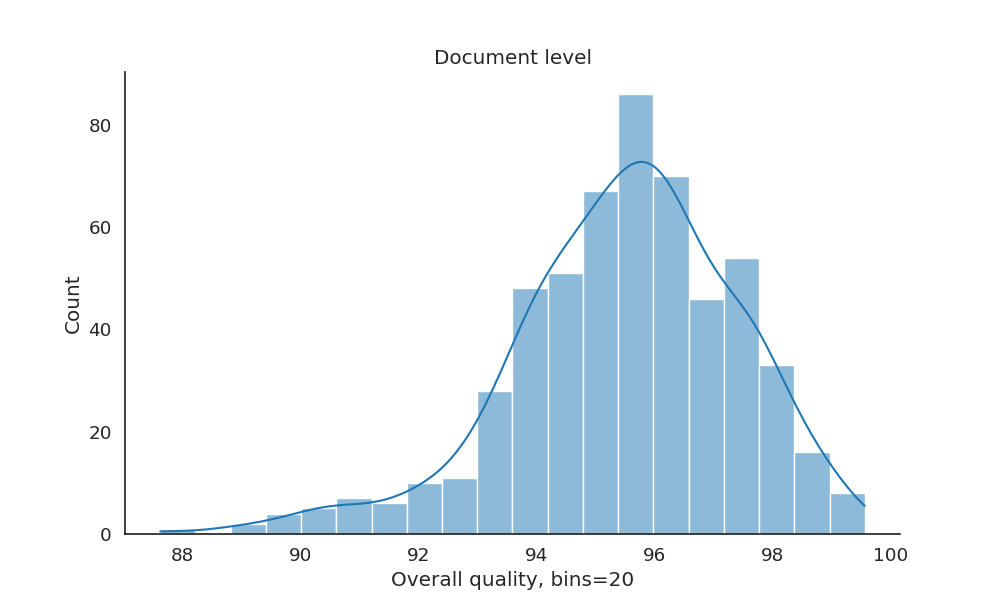
\includegraphics[width=\linewidth]{figures/err/doc-tq-noweights.png}
	\end{minipage}
	\begin{minipage}[c]{0.45\linewidth}
		\centering
		Weighted tq-score
		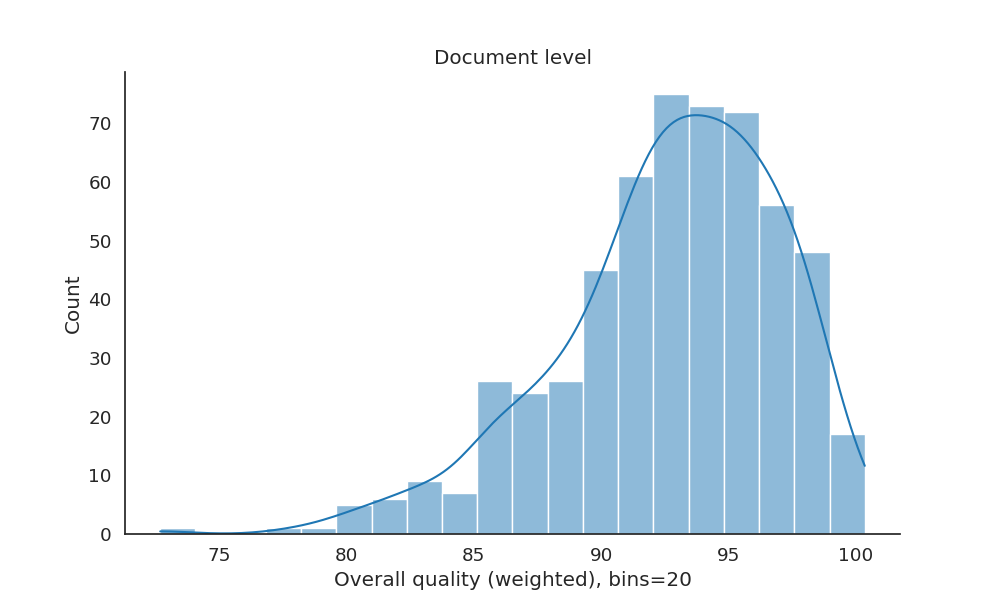
\includegraphics[width=\linewidth]{figures/err/doc-tq-major2critical5weighted.png}
	\end{minipage}	
	\caption{\label{fig:tq}Distribution of overall error-based quality scores for 553 documents}	
\end{figure}

Figure~\ref{fig:tq} and~\ref{fig:docs_fluency} show that weighting did not affect the distribution of error scores in a principled way, but weighting improved the spread of the data across the measuring scale (see limits on x-axis), which might be beneficial for machine learning experiments.

\begin{figure}[H]
	\begin{minipage}[c]{0.45\linewidth}
		\centering
		Unweighted fluency
		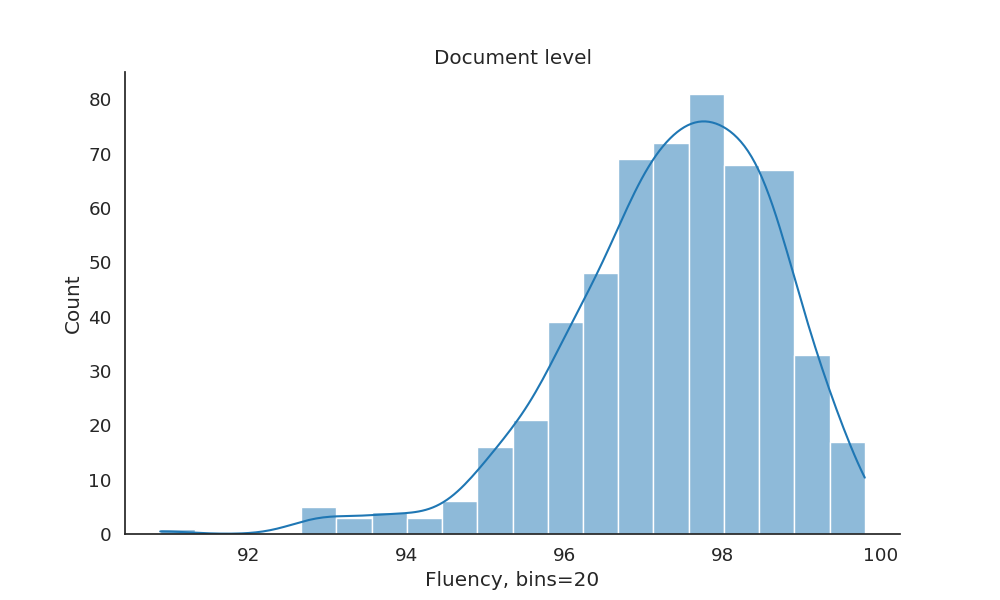
\includegraphics[width=\textwidth]{figures/err/doc-fluency-noweights}
	\end{minipage}
	\begin{minipage}[c]{0.45\linewidth}
		\centering
		Weighted fluency
		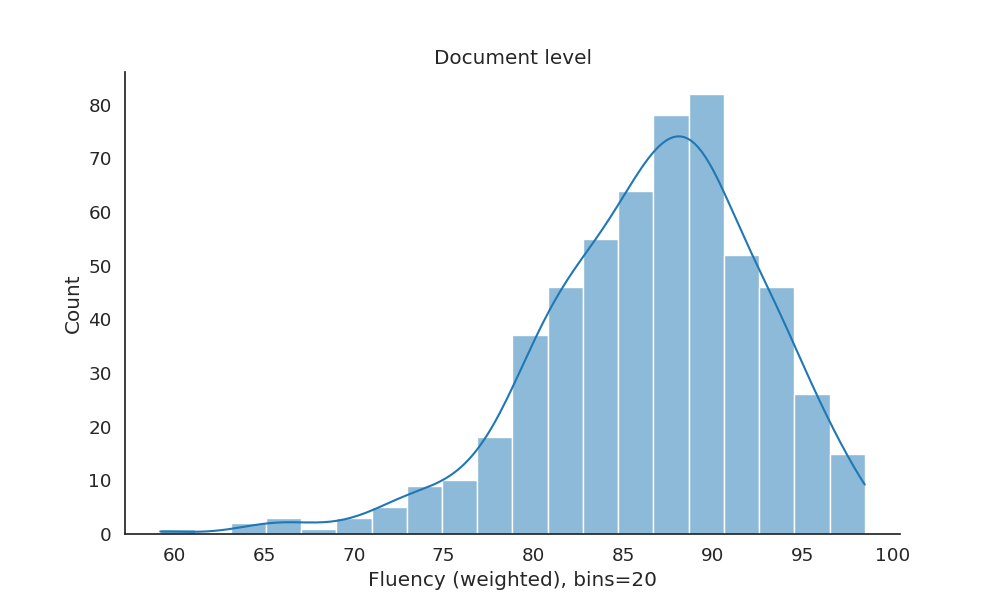
\includegraphics[width=\textwidth]{figures/err/doc-fluency-major2critical5weighted}
	\end{minipage}
	\caption{Document-level fluency scores for quality aspects}
	\label{fig:docs_fluency}
\end{figure}

\label{pg:shorts_filtered_out}
The same strategy to generate error-based scores was applied at sentence level. While producing sentence-level dataset we skipped 365 sentence pairs that were shorter than three words either on the ST or TT side of the parallel corpus. Note that the sentence-level scores reflected issues related to the document texture (cohesion, coherence, logic, etc), if those were located in a given sentence. 
Care was taken to count errors annotated as discontinuous only once.

As can be seen from the histograms in Figures~\ref{fig:sents_weighed_aspects} and~\ref{fig:sents_tq}, sentence-level scores are heavily skewed to the right, which can be a problem for ML algorithms. The distributions of document-level accuracy, fluency and overall quality scores are closer to normality.
\label{pg:skews}
\begin{figure}[H]
	\begin{minipage}[c]{0.5\linewidth}	
		\centering
		Accuracy scores
		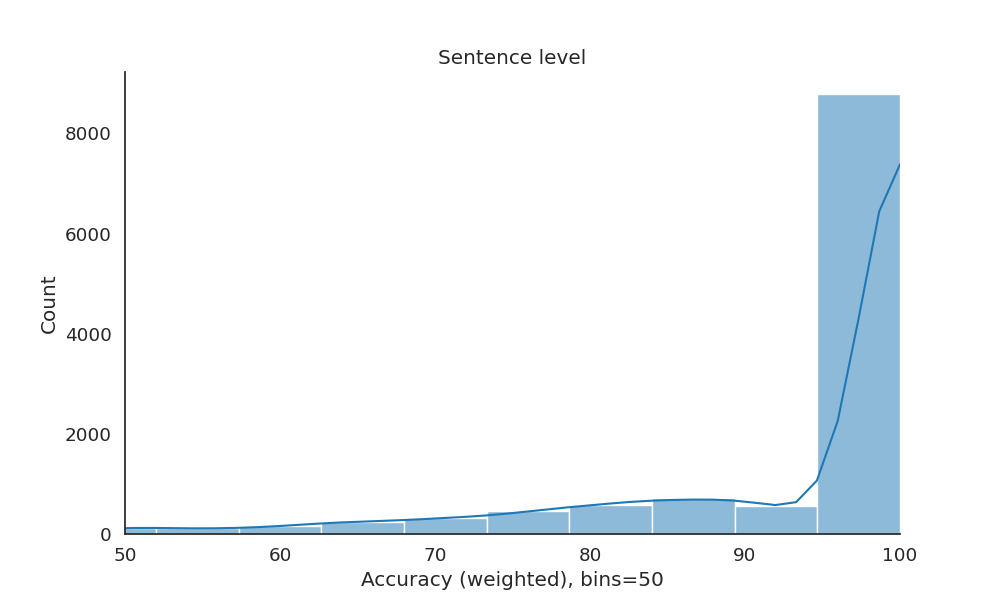
\includegraphics[width=\textwidth]{figures/err/sent-accuracy-major2critical5weighted}	
	\end{minipage}
	\begin{minipage}[c]{0.5\linewidth}
		\centering
		Fluency scores
		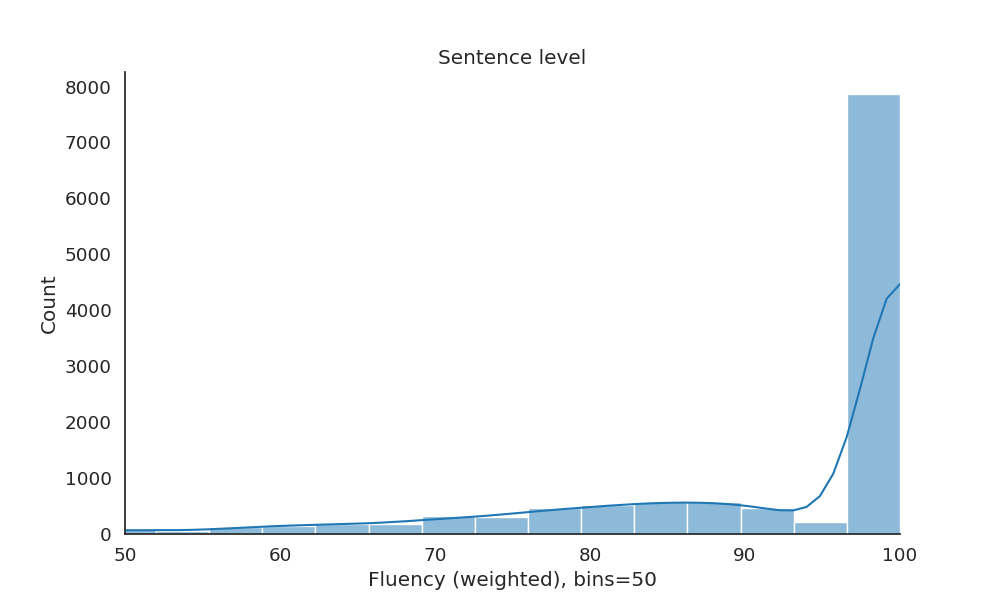
\includegraphics[width=\textwidth]{figures/err/sent-fluency-major2critical5weighted}
	\end{minipage}
	\caption{\label{fig:sents_weighed_aspects}Sentence-level weighted scores for quality aspects: accuracy and fluency}
\end{figure}

\begin{figure}[H]
	\begin{minipage}[c]{0.5\linewidth}	
		\centering
		Unweighted tq
		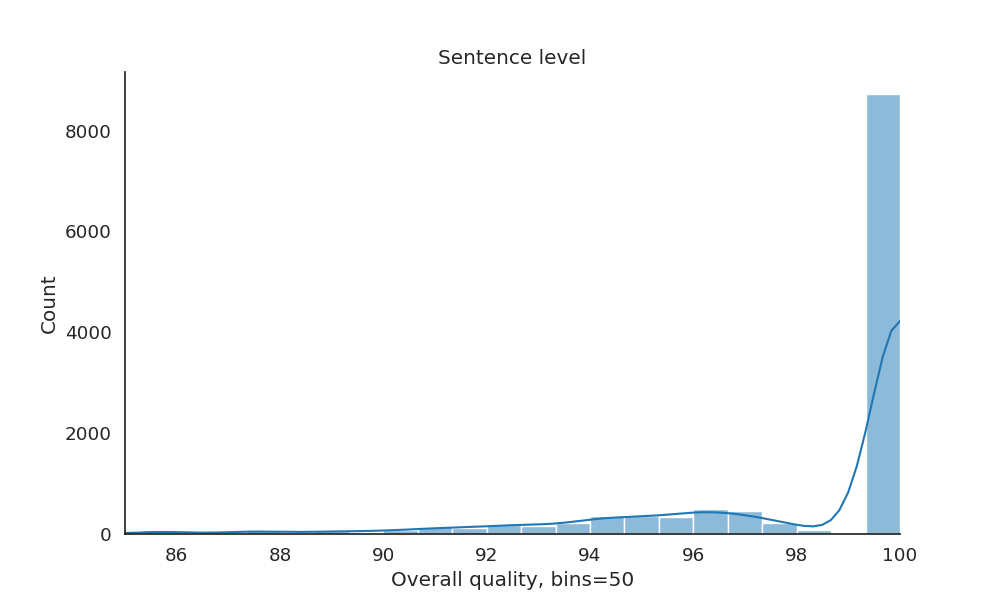
\includegraphics[width=\textwidth]{figures/err/sent-tq-noweights}	
	\end{minipage}
	\begin{minipage}[c]{0.5\linewidth}
		\centering
		Weighted tq
		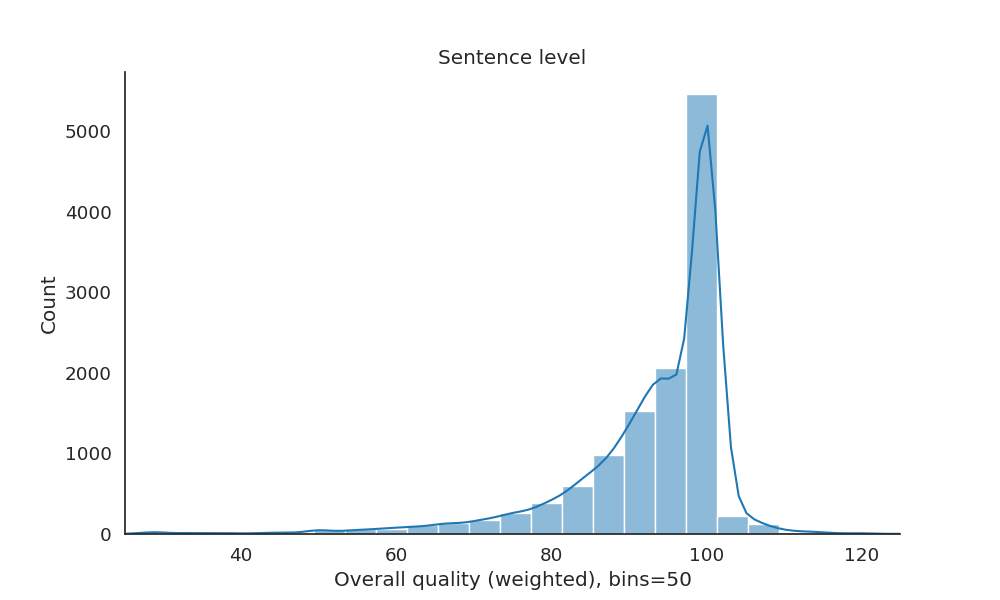
\includegraphics[width=\textwidth]{figures/err/sent-tq-major2critical5weighted}
	\end{minipage}
	\caption{\label{fig:sents_tq}Sentence-level overall quality: unweighted and weighted}
\end{figure}


\subsection{\label{ssec:da}Direct Assessment}
This section has a description of an annotation project, specifically designed to get quality labels from a controlled experimental setup, which follows the requirements and recommendations discussed above (see pages~\pageref{par:da_best}--\pageref{ssec:relval}) .
 
\paragraph{DA experimental setup and results} 
% beware! of is a very skewed output distribution of the DA scores for these particular language pairs.
The Direct Annotation experiment was organised in October 2020 to January 2021. It involved 12 final-year bachelor degree students majoring in Linguistics or Translation Studies (Russian L1, English at least B2). The participants volunteered to do the annotation as part of their internship; the arrangement was approved by the University authorities. The participants were selected from a larger pool of volunteers following the recommendation by their respective course leaders, who characterised the selected subjects as best of their cohorts (based on academic achievements in their majors). 
The students' work was graded upon the completion of the annotation tasks and a written report which contained cross-linguistic analysis of source and target texts with a commentary of translation errors. All participants were using aliases instead of real names throughout the experiment and in all communication of the results and progress. 

The experiment was set up on \textit{QuestionPro}\wlvfootnote{\url{www.questionpro.com/}} website, a flexible environment to design online surveys. Following the most recent recommendations for organising quality annotation campaigns by~\citet{Laubli2020}, an annotation task was structured to include the entire document (or coherent extract from large texts) and to present annotators with the source and the target. The annotators were asked to move a slider on a 100-point scale to indicate perceived translation quality.

At the initial stage of the project, there were separate tasks for assessing fluency (in a reference-less monolingual setting) and accuracy (in a bilingual setting). An annotator never received the same document for both settings to avoid familiarity bias. However, the results on control items with `known' quality indicated that annotators struggled with distinguishing the two aspects, and this distinction was abandoned for a syncretic quality judgment. 

The annotation task was formulated as follows: ``Read the source text. Use the slider to indicate how much you agree that the text in bold is an adequate translation of the original English segment, given the context.'' 

Before starting on their independent annotation tasks, the participants were explained the purposes of the experiment and had to complete a 30-minute questionnaire which presented them with a number of translation quality assessment tasks to ensure that they understood the key concepts and terms (e.g. adequate translation, accuracy, fluency, source, target).
Besides, the participants went through a calibration session to learn the annotation environment and harmonise the rigour of judgments, while using a slider rather than a Likert scale. 
The calibration results were discussed at a conference and distributed as a written report among the participants.

Figure~\ref{fig:da} has a screenshot of one of the assignments.

\wlvfig[0.4]{da}{Part of a bilingual document and the annotation task}

The independent work was arranged in four stages. At each stage annotators received a batch of 20 annotation tasks, one per document pair. Each complete annotation task (a parallel document of about 21 sentence pairs) was saved separately. The participants were given enough time to complete each batch and were encouraged not to do all 20 tasks in one go.

\label{pg:intersection140}
The documents for annotation were carefully selected from the intersection of the datasets with binary labels and quality scores from error annotation as shown in Figure~\ref{fig:subsets} (page~\pageref{pg:subsets}). The dataset for annotation comprised 150 multiple translations to 30 English sources, 3,849 unique sentence pairs, including spam items and one repeat document for every participant. 
Spam items were documents with artificially reduced quality to test the integrity and sanity of annotators. Repeat items were exactly the same texts offered to each annotator two months later in a different batch to measure their internal (intra-rater) reliability.

Each source text had 2-3 good and 2-3 bad translations which were never offered in the same batch. In fact, one reason to involve many participants was to avoid presenting an annotator with alternative translations of one source text, at least within one batch, to avoid familiarity bias. To achieve this, we grouped annotators into two teams of six: three translators and three linguists on each team. Each team received their own set of 75 annotation tasks, i.e parallel documents (1,936 and 1,913 sentence pairs for Team 1 and Team 2, respectively). 

To obtain trustworthy annotations, we identified most internally reliable annotators on each team who spotted the spam sentences and returned most consistent results on the repeat items presented to them in different batches. In one of the teams, only two people managed to overcome the established quality control thresholds. Therefore, we had to discard the lower-scoring rater in the other team. Those four raters were treated as interchangeable. This means that the entire dataset had double annotation, half from one team, half from the other team.
% Graham2013: to use the Kappa coefficient to compare agreement levels for the interval-level and continuous scales, we convert continuous scale scores to a target number of interval categories (p.38)
% measure the agreement AFTER standardisation: ``with inter-annotator agreement increasing by up to +0.144 when additional standardization of scores is applied''.
The inter-rater agreement for the document-level annotation achieved weighted Krippendorff's alpha\wlvfootnote{We treated 0-100-point scale as an interval scale and z-transformed values before IRR calculations as recommended in~\cite{Graham2013}} of 0.541 (140 documents, 3,224 sentence-pairs).
% 0.481 for raw scores at document level
For sentence-level, Krippendorff's alpha was 0.463 for z-transformed scores (across 3,224 instances). % 0.440 for raw scores

% 3,557 is the number of sents in 150 files before 10 dropped, there are 3318 sentences in 140 cross-annotated translations, 94 sentences were filtered out as short from sentence level dataset.
Further on, for each team we highlighted individual sentences where both raters returned scores that had more than 30-points difference. 
The raters yielded scores that were less than 30 points apart in 3,090 cases out of 3,318 true instances (sentence-pairs excluding spam and repeat items).
% on average the difference was 3.75, +/-15.73 points BEFORE reworking items. 
% 3318-3090 = 228 difference >= 30 points
The 228 sentences with over-30-points mismatch often were errors in alignment or encoding, and the raters treated them differently. In some translations by-line or date of the publication were omitted in translation, and this led to disagreements. 
%These sentences were fixed and sent for reworking to one of the more reliable raters from the other team. -- Nope, we retain them as is.

\label{pg:final_da}
To get the final scores, we averaged judgments of two raters. Following the practice adopted at \gls{WMT}, the dataset also contains the average of scores that have been z-transformed by rater using Equation~\ref{eq:zscore}. These scores are referred to as \textit{da\_mean} and \textit{da\_zmean}, respectively.

% WMT20 dataset columns: segid	original	translation	scores	mean	z_scores	z_mean	model_scores

\begin{equation}\label{eq:zscore}
\begin{split}
z = \frac{x - \mu}{\sigma} \\
\text{where $\mu$ is mean of the scores by rater,} \\
\text{and $\sigma$ is standard deviation of the respective set of scores}
\end{split}
\end{equation}

Sentence-level datasets with scores from error annotation and from DA experiment were combined to get one dataset with five primary scores (accuracy, fluency, tq, da\_mean, da\_zmean) for intersecting items to enable comparison of the quality scores generated by various methods. 

There were 94 short DA-annotated sentences filtered out from the error-annotated dataset as explained on page~\pageref{pg:shorts_filtered_out} (e.g. \textit{Liquid Gold} -- \cyrillictext{Вода по цене золота} [Water at the price of gold] (RU\_1\_325\_7\_s8); \textit{Right?} -- \cyrillictext{Согласны?} [Agree?] (RU\_1\_268\_4\_s45)).
% Product Placement: On Broadway  Продакт-плейсмент на Бродвее 36.0   100.0
Those sentence pairs were removed from the sentence-level (but not from the document-level!) dataset to ensure consistency.
% Document-level DA scores are calculated from the complete documents.
\begin{table}[H]
	\centering
	\begin{tabular}{l|c|c|cc}
		\toprule
		
		& documents & sentences & \multicolumn{2}{c}{tokens} \\
		&      &        & EN      &  RU \\
		\midrule
		error annotated & 553  & 12,369 & 250,916 & 225,782 \\
		\hspace{1em} inc. with DA & 140  & 3,224 & 62,441 & 57,102 \\
		\bottomrule
	\end{tabular}
	\caption{\label{tab:sent_err_da} Parallel subcorpora with error and DA annotation}
\end{table}

\vspace*{-1em}
Table~\ref{tab:sent_err_da} brings together the basic quantitative parameters of the dataset with error annotation and DA annotation.
% it was impossible to put sentences with DA and sentences with err-scores into the same df, because a reliable intersection between sent_ids, holding the same (matching) tsent was only 774 tsents out of around 3000. This is because sent_ids were added to err and da texts separately, they went through alignment separately, we deleted items with >= 30 points diff between rater1 and rater 3 (228)

% sent_ids in err and da datasets are mapped to the ame sents, the literal string mismatch is due to the absence of punctuation in "item". We don't use this column anyway.
\label{pg:da_score_hists}
\begin{figure}[H]
	\begin{minipage}[c]{0.5\linewidth}
		\centering
		Document-level
		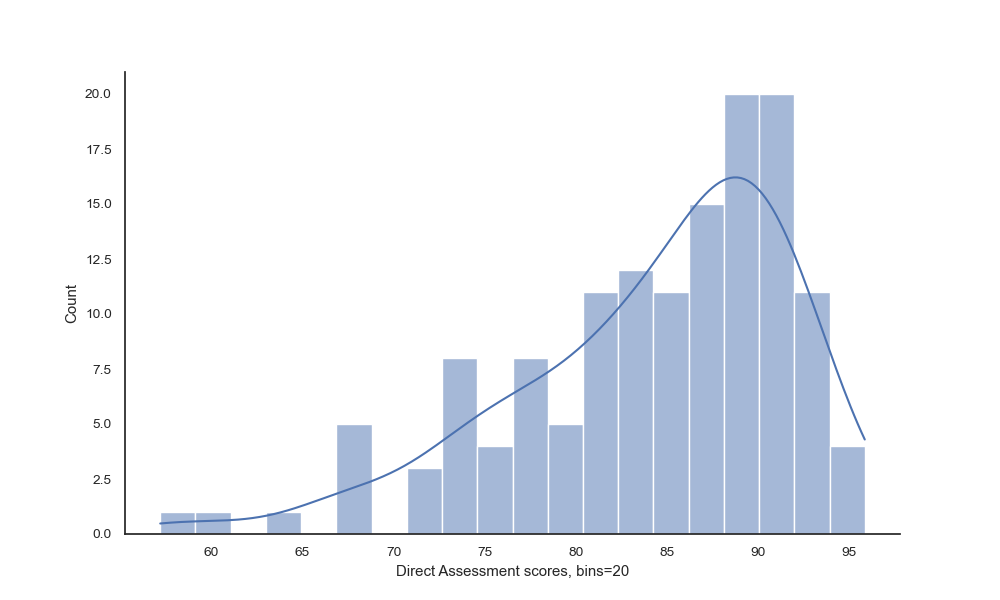
\includegraphics[width=\linewidth]{figures/da/doc-da-score-distribution}
	\end{minipage}	
	\begin{minipage}[c]{0.5\linewidth}
		\centering
		Sentence-level
		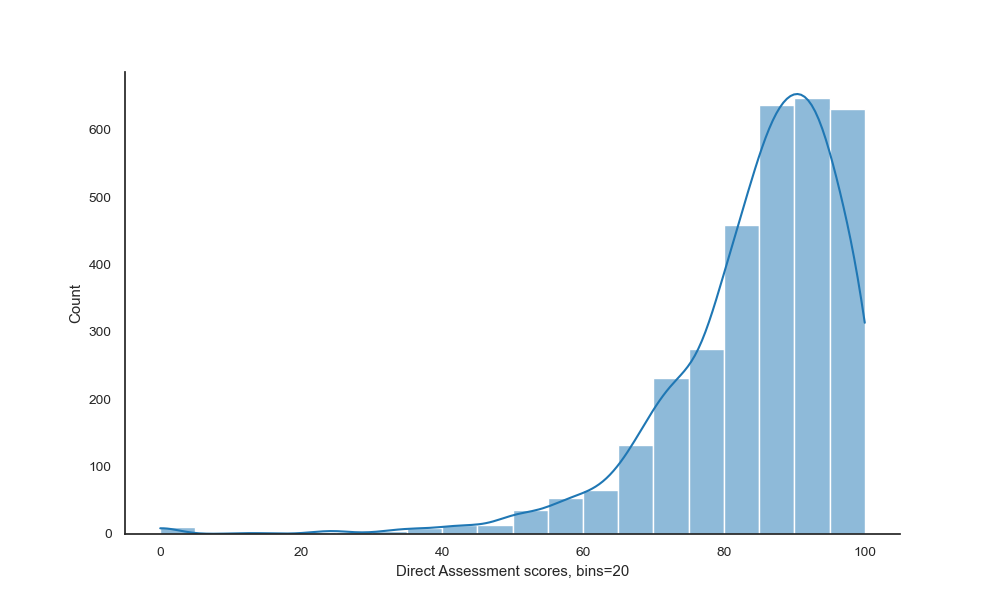
\includegraphics[width=\linewidth]{figures/da/sent-da-score-distribution}
	\end{minipage}
	\caption{\label{fig:da_scores}Distribution of scores from DA experiment for documents and sentences}	
\end{figure}

\vspace*{-1em}
We provide a visualisation for the distribution of DA scores at document- and sentence-level in Figure~\ref{fig:da_scores}. Similar to scores from error annotation, sentence-level dataset has a more noticeable right skew: there are many more sentences with high-quality scores than with low-quality scores. 


\section{\label{sec:sum4}Summary}

This chapter presents the theoretical concept of quality in translation and practical approaches to quality quantification. 
It is focused (i) on automatic quality estimation methods for machine and human translation (Sections~\ref{ssec:mtqe} and~\ref{ssec:htqe}) and (ii) on the best practices in producing manual quality benchmarks for NLP experiments (Section~\ref{sec:ass}). The final section of the chapter has a description of annotation procedures used to obtain quality labels and score in this research (Section~\ref{sec:mygold}).

In \gls{TS}, quality is defined with the emphasis on extralinguistic context, including the purpose of translation, intended audience and medium (pragmatic aspect of quality, usually referred to as adequacy). MT research is mostly focused on accuracy and fluency aspects, where accuracy is viewed as (lexico-)semantic similarity between ST and TT, and fluency is approached as readability/grammaticality in the TL. The relative nature of quality was highlighted with regard to three factors, including the purpose of assessment, parameters of communicative situation with translation and comparison with alternative translation candidates. 

Comparing approaches to quality in HT and MT, we have emphasised the limitations of some MT methods due to the predominantly document-level nature of HT, greater variation of language and higher quality expectations attached to HT.

Section~\ref{sec:qe} characterises translation quality estimation as a computational linguistics and NLP task in MT, alternative to reference-based quality evaluation. It can be formulated at various language levels, with sentence level being more practicable for the current MT systems and language representation models. For anyone with the TS background, the idea to assess translation quality on isolated sentences is questionable. 
%Quality estimation tasks predominantly use continuous scores as learning targets. In this case the evaluation studies rely on correlation coefficients and error rate metrics to compare the performance of various methods. When quality of translations is captured by discrete labels, systems' evaluation is based on typical ML classification metrics: accuracy, precision, recall and F-score. 

This chapter offers an overview of the current best-performing approaches in MTQE and summarises the two projects that attempted to extend MT estimation methods to HT. 
Document-level HTQE based on a careful selection from a elaborate set of 360 types of hand-engineered surface features achieved Pearson's $r=0.72$ outperforming \textit{QuEst++} on the dataset proposed in Yuan's \citeyear{Yuan2018} research. In their experiments feature-learning approach was inferior to explicit features at sentence level. However, a critical analysis of their learning setup (in particular, very repetitive translations for a few STs) warrants doubts about robustness of this approach.
The other research casts HTQE as an unsupervised sentence-level task based on learning similarity between ST and TT.
We demonstrate that current state-of-the-art in MTQE relies on pre-trained contextualised embeddings fine-tuned on quality labelled data, and researchers' attempts are focused on explainability. Document-level MTQE task waits for further advances in technology to be successfully tackled and builds appropriate datasets meanwhile. 
We include a critical description of a popular MTQE feature set from \textit{QuEst++} used as a baseline in this research.  

The last two sections of this chapter discuss the second component of any quality estimation task -- quality labels. 
We presented a fairly detailed analysis of reliability and application of the major assessment methods in HT (rubrics and error annotation) and in MT (error annotation, direct assessment, post-editing). It has been repeatedly emphasised that when it comes to collecting human judgment about translation quality, it is best to resort to professional expertise, provide a rigorously formulated definition of quality for each text type/communicative situation and have a calibration strategy in place. The latest recommendations also require sentences to be assessed in the true document order.
In MT there is more awareness that these methods capture various dimensions of quality, and there is more pessimism about getting humans to agree about quality. It is obvious that in MT there is a pressure to adjust quality benchmarking methods to the changes in MT quality delivered by the introduction of NMT. 
%In our opinion, lower inter-rater reliability results in MT can be explained by non-professional annotators, who look at an isolated sentences. 
We tend to agree that the distinction between aspects of quality (accuracy and fluency) is even more difficult to capture in an annotation experiment than theoretically. 

While describing the best practices in producing quality benchmarks in MT, we focus technical details, such as the choice of top-level error categories, use of severities, ways to convert error statistics to actual quality scores and limitations of popular annotation environments. 
A separate subsection discusses organisation of reliability studies for various annotation setup. We note that measuring IRR for error annotation or post-editing is particularly difficult because ideally it should involve taking into account the agreement about the location of the annotated spans and their categorisation. Further caveats, heeded in our own experiments, include the recommendation to use Krippendorff' coefficient in IRR studies and to apply metrics to z-transformed (standardised) DA scores instead of absolute values. 
%It was also repeatedly shown that the outcomes of supervised ML experiments are contingent on the distribution of scores in the dataset. 

Finally, we provided detailed descriptions of three annotation procedures used to obtain or verify various quality labels/scores in our datasets. The results were reported in terms of IRR and scores distribution at document and sentence levels. We demonstrated that in our various experiments the agreement between university translation teachers (nominal-scale assessment and error annotation) and final-year under-graduate students (DA experiment) as raters ranges from 0.467 to 0.734 in various settings, with the lowest result seen for sentence-level DA by students.

\chapter{\label{cha:translationese}Translation Detection}
This chapter examines the strength of the investigated hypothesis that the amount of translationese manifested in a translation can be a good predictor of the level of professionalism and quality. 

Sections~\ref{sec:detect} and~\ref{sec:bestof} have the results of translationese classifications, where translations (professional or student) are distinguished from non-translations to demonstrate that the selected hand-engineered features are, in fact, effective to capture translationese. 
%To make sure that the proposed features are competitive in a translation detection task, their performance is contrasted with other representations including content-dependent features. 
If our hypothesis stands, we can expect that the more salient translationese indicators will also be good quality predictors. 
To shed more light on feature subsets and individual variables that can be considered most effective in capturing translationese, we analyse outcomes of automatic feature selection and perform univariate analysis for the three proposed types of features in Section~\ref{sec:bestof}.

The chapter opens with a description of the experimental setup for classification tasks including details on learning algorithms, generation of alternative representations and numeric data preprocessing (Section~\ref{sec:my_classifiers}).

\section{\label{sec:my_classifiers}Experimental Setup}

\paragraph{Dataset and proposed translationese indicators} The input to classifiers was arranged as a table of 3055 rows by 167 columns. In that table each row represented a document (including sentence-aligned source texts for parallel subcorpora). Columns stored three labels, six meta descriptors of each document-instance (document ID, language, word count, number of sentences, raw text and lemmatised text) and 158 hand-engineered numeric features from the attempted manual feature sets. 

The labels reflected pairs of categories, listed below to introduce their shorthand names used throughout the experiments:

\begin{description}\compresslist{}
	\item[pro vs ref:] professional translations vs non-translations;
	\item[stu vs ref:] student translations vs non-translations;
	\item[stu vs pro:] student translations vs professional translations (see Section~\ref{ssec:var} in Chapter~\ref{cha:pro_qua});
	\item[bad vs good:] categorial document-level quality labels from holistic assessment of student translations verified in a separate annotation effort (results on this dataset appear in Section~\ref{ssec:bin}).
\end{description}

Throughout the rest of the thesis, linguistically-motivated translationese-aware feature sets are represented as follows:
\begin{description}\compresslist{}
	\item[UD:] 60 features extracted from Universal Dependencies annotations (see Section~\ref{ssec:ud});
	\item[collgram:] 24 features representing abstract collocational properties of texts (see Section~\ref{ssec:coll});
	\item[ngram:] 10 features from 1-2-3-gram frequency lists and from n-gram-based language models (see Section~\ref{ssec:ngram});
	\item[all:] combination of the above feature sets (94 features).
\end{description}  

%Adding actual raw and lemmatised texts into the table and setting the random seed helped to ensure that the same instances were found in the same order in the same folds regardless of the representation used: manual features or vectors from pre-trained embedding models.

\paragraph{\label{pg:vectors}Alternative document representations} To demonstrate the competitiveness of hand-engineered features, we compare them with a number of alternative representations. 

The chance-level baseline was calculated using a stratified strategy, which ignored the input features altogether. The results were based on randomly assigned class value to each feature/component in a document vector respecting the class distribution in the training data.

The hand-engineered features were relatively content-independent. Their performance was contrasted to surface-feature-based \gls*{tf-idf} representation and to text vectors generated by mean-pooling of embeddings from several Transformer models (see page~\pageref{pg:embeddings}).
The vectorisation setup in each case was implemented as follows.

\label{pg:tfidf_meth}
\textit{Tf-idf} is a numeric representation for documents which uses weighted frequencies of a corpus vocabulary items as vector components. Those vectors were calculated using a dedicated \textit{scikit-learn} utility. We used all available documents in the Russian language as the underlying corpus. 
To reduce vocabulary size and increase informativity of this representation, the corpus was lemmatised. All proper names and their sequences were replaced with a \textit{PROPN} tag (e.g \textcyrillic{\textit{говорит Максимилиан Чуперски}} [says Maksymilian Czuperski] --> \textcyrillic{\textit{говорить PROPN}}). All digits were replaced with \textit{X} (e.g. \textit{12 октября 1982; 2,5;  1980-е} --> \textit{XX October XXXX; X.X; XXXXs}). The vocabulary was built to include word unigrams, bigrams and trigrams. The vector size was limited to 5000 most frequent corpus vocabulary items. Other hyper-parameters were set to the default values from the library. 
% we should have excluded items in English as simple give-aways for translations vs non-translations, because translatons often retain the proper names in the SL in parenthesis, and those were not tagged as PROPN but as foreign_word.

We also used four pre-trained contextualised embedding models to infer vectors for documents in our experiments. These models aim to generate distributed representations of document meaning (in a broad sense) and are content-dependent. The models are open-source and freely available from the \textit{HuggingFace} repository.

We selected the models that were trained to solve various NLP tasks deemed more suitable for our purposes. The list below gives a brief description of each model. 
\label{pg:embeddings}
\begin{description}\compresslist{}
	\item[stsb-xlm-r-m:] a multilingual model\wlvfootnote{\url{huggingface.co/sentence-transformers/stsb-xlm-r-multilingual}} trained using Sentence-BERT (SBERT), a~\gls{SOTA} framework to compute sentence representation~\cite{Reimers2019}. SBERT is a generic name for contextualised embedding models fine-tuned on various sentence-level tasks such as question-answering, sentiment, paraphrasing, etc. The model is a multilingual XLM-R fine-tuned on \gls{STS} task;
	
	\item[TQmono-m:] a cross-lingual model for many languages\wlvfootnote{\url{TransQuest/monotransquest-da-multilingual}} trained by the more successful architecture from \textit{TransQuest} package~\cite{Ranasinghe2020}, to solve MT quality estimation task based on DA scores;
	% these models generate word embeddings that are mean-pooled under the hood by SentenceTransformers library 
	
	\item[ruRoberta:] a dedicated Russian model\wlvfootnote{\url{huggingface.co/sberbank-ai/ruRoberta-large}} trained as a full-mask language model using \textit{RoBERTa}, an optimised BERT transformers training method proposed by~\citet{Liu2019};
	
	\item[mdeberta3:] a multilingual version of \textit{DeBERTa}~\cite{He2021}, an improvement on \textit{BERT} and~\textit{RoBERTa} word embedding architectures, trained on 2.5T CommonCrawl corpus for 100 languages \wlvfootnote{\url{huggingface.co/microsoft/mdeberta-v3-base}}. At the time of writing, it is \gls{SOTA} in word-level representation learning. 
\end{description}

The first two models generate sentence embeddings, while the last two output word embeddings, which were averaged to get sentence embeddings. Further on, the sentence embeddings were mean-pooled to obtain document vectors. 
Note that in most experiments we might not have enough datapoints to train these representations further on the labels available in our tasks in a fine-tuning setup. % Methodologically, we use transfer learning approach? 
%768-dimensional vector

For all experiments and representations, the input data was transformed with \textit{scikit-learn Standard Scaler}. This function standardises the values of each feature column-wise (i.e. independently) to have zero mean and unit variance of 1. It helps to put all features on the same scale regardless of the original measurement unit, and avoid the situation when features with large variance dominate the learning process overshadowing the differences on other features.

\paragraph{Algorithms} Both classification and regression experiments (reported in Chapter~\ref{cha:pro_qua}) are based on \gls{SVM} algorithm as implemented in \textit{scikit-learn}, a Python library for machine learning. 
This algorithm was shown to be superior to tested alternatives for translationese classification in a number of research projects (see, for example,~\cite{Ilisei2010}). It is also known to be robust to high-dimensional datasets where the number of instances is similar or even smaller than the number of features.

This research is focused on testing the hypothesis whether translationese indicators are correlated with translation quality, and on exploring the relations between a number of diverse representations and quality labels. Our aims did not include achieving the best performance possible for given datasets, therefore, the results for various SVM kernels and other parameters of algorithms that can be discovered through optimisation studies are omitted. 
Instead, the classification experiments are based on a linear kernel SVM and regularisation parameter $C=1.0$ (default for SVM \textit{scikit-learn} setting).

SVM uses pairwise distances between the datapoints from given categories and identifies instances with most similar vectors (called \textit{support vectors}). Then, it calculates a maximum hyperplane separating these support vectors, by assigning positive or negative weights to features to put instances on the required side of the hyperplane and to reduce algorithm error. Instances that are found on the opposite sides of the hyperplane are assigned to the respective categories. 
\textit{C} parameter is the cost of misclassification, or tolerance for errors. Higher \textit{C} values lead to fewer errors in the training set, and to a more overfit model, which would not generalise well. It will result in poorer performance on a test set.
%
%Although the datasets in our experiments are reasonably well-balanced we kept the \textit{class\_weight} parameter of the algorithm set to \textit{balanced}. 

For quality control, we implemented a simple sequential neural model to replicate the performance of SVM-based classifiers on exactly the same inputs. The neural model~\label{pg:neural} was designed using \textit{Keras} \gls{API} integrated into \textit{TensorFlow 2.0} (tf.keras)\wlvfootnote{Both \textit{TensorFlow} (\url{github.com/tensorflow/tensorflow}) and \textit{Keras} (\url{keras.io/}) are open-source libraries for deep learning with Python.}. The neural model used document vectors as input and was compiled with two dense (i.e. fully-connected) hidden layers. The first layer was  made of 16 neurons and was activated with \gls{ReLU} function, which output zero for negative input values and returned the input directly if the input was positive. The output layer for the classification task was activated with a \textit{sigmoid} function, which mapped all inputs in the real number domain into the range of 0 to 1. % It transformed input values that were much larger than 1.0 to 1.0, values much smaller than 0.0 were snapped to 0.0. 
This layer output the probability of a test instance belonging to a positive class. The threshold of 0.5 was used to obtain the model predictions of binary categories. 
%For the regression task, we use \textit{linear} activation function, which scales each input by a learnt factor and assumes linear relation between inputs and targets. 
% mean absolute error can be used as loss function for regression
The model was compiled with \textit{binary cross-entropy} as loss function for the classification tasks. \textit{Adam optimiser} was used for gradient descent calculations; each experiment was set to run for 10 epochs with batch size 8. The learning process was monitored with an \textit{EarlyStopping} class. It was set to keep track of accuracy across 10 training epochs for each run of the experiment. The training stopped if the gain in the algorithm performance was less than 0.0001 for three consecutive epochs. 

Another standard ML setting, which contributes to better generalisation of the models, especially with high-dimensional data, is cross-validation. 
The data was split 10 times into a training set and a test set in a cycle, respecting the balance of categories, so that each instance appeared in a test set at least once. We report the averaged results and their \gls{STD} across 10 runs (folds) of each experiment. 
%All scores are expressed as percentages. 

%We use the standard evaluation metrics for classification problems as described in Section~\ref{ssec:task} (page~\pageref{pg:eval_setup}). 

\paragraph{\label{pg:eval_setup}Evaluation setup} 
%Evaluation setups in this thesis depend on the type of labels used. 
In Chapters~\ref{cha:translationese} and~\ref{cha:pro_qua}, the tasks formulated as \textit{classification problems on discrete labels} were evaluated on accuracy, precision, recall and F1-score.
% classeval.wordpress.com/introduction/basic-evaluation-measures/ 
% A binary classifier predicts all data instances of a test dataset as either positive or negative. This classification (or prediction) produces four outcomes – true positive, true negative, false positive and false negative.
% A confusion matrix is formed from the four outcomes produced as a result of binary classification.

For completeness of this description, let us define \textit{accuracy} as the number of all correct predictions divided by the total number of instances in the dataset, \textit{recall} % aka sensitivity or true positive rate
as the number of correct positive predictions divided by the total number of instances belonging to a class (positives), and precision % aka positive predictive value
as the number of correct positive predictions divided by the total number of positive predictions.
F1-score is a harmonic mean of precision and recall, calculated as shown in Equation~\ref{eq:f1}. % as opposed to weighed F measure where preference can go to either precision or recall to get the result. 
\begin{equation}\label{eq:f1}
	F1 = 2 * (precision * recall) / (precision + recall)
\end{equation}
The datasets were reasonably balanced, so F1-score was calculated independently for each class and then averaged across classes (macro-averaged F1-score). %treating both classes equally

% A macro-average will compute the metric independently for each class and then take the average (hence treating all classes equally), whereas a micro-average will aggregate the contributions of all classes to compute the average metric. In a multi-class classification setup, micro-average is preferable if you suspect there might be class imbalance (i.e you may have many more examples of one class than of other classes).

%Our experimental Chapters~\ref{cha:translationese} and~\ref{cha:pro_qua} report accuracy, precision, recall and F1-scores as classifiers' performance measures, expressed as percentages, and \gls{STD} (a measure of variance) across 10 folds in a cross-validation setting.
% STD is known as theta $\theta$ and $\theta^2$ is a measure of variance

%\citet{Specia2018a} recommended to supplement them with graphical representation of a classifier's performance with \gls{ROC} curves, which visualise the relation between sensitivity (the true positive rate) and specificity (the true negative rate) for different thresholds to find the optimal equilibrium between the highest true positive rate and the lowest true negative rate, represented by a curve reaching for the upper-left corner. To report this balance as a number, \gls{AUC} statistic is used. AUC values vary in the range from 0 to 1, where 1 is AUC for a perfect classifier.
% http://navan.name/roc/
%
%For \textit{regression models on continuous scores}, \textit{Pearson's $r$ correlation coefficient} proposed by~\cite{Graham2015r} was used. This coefficient measures linear correlation between two variables/datasets ($x$ and $y$) and is estimated as the ratio of covariance of the variables to the product of their \gls{STD}s (see Equation~\ref{eq:pearson}, where $n$ is the size of the paired datasets, and $\overline{x}$ and $\overline{y}$ are means of values in each respective dataset). % also refered to as least-squares fit, minimizing the sum of the squares of the residuals (diffs between predicted and true labels)
% the ratio between the covariance of two variables and the product of their standard deviations; thus, it is essentially a normalized measurement of the covariance

% Pearson's correlation coefficient, when applied to a population, is commonly represented by the Greek letter rho and may be referred to as the population correlation coefficient or the population Pearson correlation coefficient. Results for a given pair of random variables is represented by rho ρ

% Pearson's correlation coefficient, when applied to a sample, is commonly represented by r and may be referred to as the sample correlation coefficient

% as presented in the documentation of def pearsonr(x, y) in scipy.stats 
%r = \frac{\sum (x - m_x) (y - m_y)}{\sqrt{\sum (x - m_x)^2 \sum (y - m_y)^2}}
%\begin{equation}\label{eq:pearson}
%	r_{xy} = \frac{{}\sum_{i=1}^{n} (x_i - \overline{x})(y_i - \overline{y})}
%	{\sqrt{\frac{\sum_{i=1}^{n} (x_i - \overline{x})^2}{n}}\sqrt{\frac{\sum_{i=1}^{n}(y_i - \overline{y})^2}{n}}}
%\end{equation}
%
%The coefficient value lies in the range from -1 to 1, where a value of 1 represents a perfect positive relationship, -1 is a perfect negative correlation, and 0 indicates the absence of a relationship between variables. 
%In QE tasks, the variables are gold scores generated from human annotations and scores predicted by models for all test instances. 
%
%%\todo[inline]{An underlined variance-related effects; and there is some other formula for eq:pearson at the bottom of the page by An}
%The correlation coefficient is complemented by non-parametric \gls{RMSE} measure. Unlike Pearson's $r$, this metric does not make the assumption of normal distribution of values, and would penalise predictions for instances which deviate too much from gold standard. 
% \cite[p.58]{Specia2018a} ``This means that, if the predictions of a given QE model show high variance, it will lead to a high MAE, even though the distribution ofthe predictions follows the distribution ofthe true labels.''
%\gls{MAE} and \gls{RMSE} focus on the scale of deviations of generated predictions from the gold scores instead of reflecting the similarity of distributions between predicted and true labels measured by \textit{Pearson's coefficient} under the assumption of normality.

%A variant of Spearman's $r$, a rank-based version of Pearson's correlation coefficient, is used for WMT ranking tasks. It is a non-parametric test that aims to measure monotonicity of the relationship between two variables, given the difference in ranks between predicted and true labels. % reflects dependence between ranked variables, maybe a non-linear relationship
%
%Pairwise comparisons of participant systems predictions to human ranking was also measured as Kendall's $\tau$, i.e. the difference between concordant and discordant pairs normalised to total pairs.
% Why 6? simply out: it is a way to remove rho’s dependency on the number of data points N and rescale to the interval [-1, 1].
% michaelpoli.medium.com/spearmans-rho-why-the-6-866a7020c004

%\begin{equation}\label{eq:spearman}
%\rho = 1-{\frac {6 \sum d_i^2}{n(n^2 - 1)}}
%where
%d = the pairwise distances of

\paragraph{\label{par:featanal_meths}Feature Analysis Methods}
% correlation matrix for feature selection and analysis: https://medium.com/geekculture/feature-selection-in-machine-learning-correlation-matrix-univariate-testing-rfecv-1186168fac12
Detection of the best translationese indicators was performed using \gls{RFE} technique. 
%We believe that some features might form functional subsets that would perform better together. 
In particular, \gls{RFECV} method was used to retrieve a dynamic set of most informative features of size N for each dataset. 
\gls{RFECV} applies an algorithm (a linear SVM, in our case) to a feature space reduced by one feature with the least importance in each subsequent run of the experiment. The importance of features is established using weights assigned by the algorithm. In our experiments, the algorithm iterated N in the range [3 : size of the feature set], performed 5-fold cross-validation on each N and returned N with the highest mean F1-score across all folds. 
%The process is continued to obtain the best performance across several cross-validation folds (five, in our case). % We scaled each features before selection to have zero mean and variance of 1. 

Weights assigned by linear-kernel SVM (and their visualisations) were used in univariate feature analysis. According to explanations in~\citet{Volansky2015}, high feature weights are a good indication of a significant difference between the two classes, but lower feature weights might not mean lack of discriminative power because feature weights can be reduced taking into account possible inter-dependencies among features in the feature set.  

Apart from providing information about the more salient linguistic properties of each category, feature selection allows to reduce the feature space by removing noisy features (if any), which might lead to an increase in the algorithms performance.
%Feature selection is applied to the most effective hand-engineered (interpretable) feature sets only.

To establish major trends in translational behaviours that could be associated with the observed linguistic properties of translations, we developed \textit{a sequence of statistical univariate tests} that described the pairwise differences between source texts, translations and non-translated TL reference.
Non-parametric statistical tests were selected in all cases, because the values of most features were not normally distributed for either of the document categories. For example, there were only 12 features in non-translated subcorpus (out of 94 total) where the null hypothesis of normal distribution was not rejected based on \textit{Shapiro-Wilk test}, a statistic test of normality.
For many manual features, the compared categories of documents also had unequal variances.   
\textit{Bartlett statistic}, which tests for homogeneity of variances across two samples, revealed that there were 68 feature with unequal variances in the translationese classification experiment based on professional translations, for example. 

These peculiarities in the distributional properties of features also explain the choice of \textit{RFE} algorithm over \textit{ANOVA} for feature selection. The latter compares between-categories and within-categories variation, and assumes normal distribution and equal variances between samples.

Statistical significance was tested using \textit{two-tailed Mann-Whitney U Test for independent samples} and \textit{Wilcoxon signed-rank test for paired samples} as a non-parametric alternative for data that violates the assumption of normal distribution made by Student's t-test.

Additionally, the strength of the relationship between each variable (feature) and target labels was measured using 5-fold cross-validated \textit{logistic regression} which returned macro F1-scores in the classification setup. 
% we cannot use Spearman with 0, 1 labels as it relies on differences in ranks
The choice of the method is explained as follows. \textit{Cohen's D} effect size metric or regular correlation coefficients cannot be used to estimate the association between a continuous variable and a binary categorical variable, because it is impossible to calculate the covariance in this setup. The use of a classifier as an association metric builds on an assumption that if a continuous variable can accurately predict a categorical variable, they can be considered correlated. 

Scatter plots and line plots were used to visualise the results of \gls{PCA} for some of our representations. By analysing covariances between features, PCA attempts to reduce multidimensional data to a few new features that aggregate maximum information of the original representation. Although dimensionality reduction simplifies the relations between datapoints, it can be useful to visually study how well each representation captures the distinction between categories. 

In the tables, the highest results for manually engineered feature sets are shown in bold and the highest results for content-dependent classifiers appear in a box. The highest observed results are defined as the results that were not significantly outperformed by any other model in that category at the confidence level of 0.05, while being greater than the numbers returned by other models. 
%All textual examples in Chapters~\ref{cha:translationese} and~\ref{cha:pro_qua}, unless indicated otherwise, are taken from student translations. 

\section{\label{sec:detect}Translationese Classifications}

This section presents the results of translationese classifications on professional and student translations. The quality of these classifications indicates how well a given feature set or representation can distinguish translations from non-translations. 

Tables~\ref{tab:pro-ref} and~\ref{tab:stu-ref} aggregate results for a linear SVM classifier on three distinct hand-crafted delexicalised feature sets and their concatenation (\textit{all}) for professional and students translations, respectively. 
They are put into perspective of chance level and the performance on \textit{mdeberta3} vectors, the best-performing content-dependent classifier.
This is done to demonstrate the achievable in our setup, and to answer the question raised in \citet{Hu2021} about the level of accuracy that is high enough to accept a feature or a feature set as discriminative. Statistical tests showed that there were no statistically significant differences between the performance on \textit{mdeberta3}, on the one hand, and on either \textit{ruRoberta-large} or on \textit{tf-idf}, on the other hand. For considerations of space, the results on \textit{ruRoberta-large} and \textit{tf-idf} are omitted.
%Note that most of translationese indicators proposed by~\citet{Volansky2015} (and used as a baseline in some translationese research) were implemented in this study and included in either \textit{UD}, \textit{collgram} or \textit{ngram} feature sets.  

Results for a neural classifier (see description at page~\pageref{pg:neural}), which was run in the same settings as an alternative for a linear SVM, appear in Appendix~\ref{appx:neural_res}. Systematic comparison between the SVM and neural classifier showed that out of 40 settings across various feature sets in four binary classifications, statistically significant differences between the algorithms were observed in only four cases (as measured with a two-sided t-test using F1-scores from 10 cross-validation folds, at confidence level $\alpha=0.05$). It confirms that in terms of learnability, SVM achieved a reasonable performance level in all tasks. 

Generally, both translation varieties were easily separable from originally-authored document on all attempted representations. Both lowest and highest F1-scores were seen on student translations: 65.63\% on \textit{collgram} feature set and 98.36\% on \textit{mdeberta3} vectors. 

Structural morphosyntactic classifiers (UD) with linear SVM kernel demonstrated competitive performance and returned macro F1-score of 90.22\% and 88.96\% for professional and student translations, respectively.

\begin{table}[H]
	\centering
	\begin{tabular}{p{2.9cm}|llll}
		\toprule
		& Accuracy        & Precision       & Recall        & F1              \\
		\midrule
		chance          & 47.72 (+/-5.93) & 47.72 (+/-5.93) & 47.70 (+/-6.00) & 47.58 (+/-5.95) \\
		\midrule
		UD              & 90.34 (+/-2.73) & 90.51 (+/-2.59) & 90.32 (+/-2.98) & 90.22 (+/-2.81) \\
		collgram        & 70.82 (+/-5.11) & 71.15 (+/-5.09) & 71.16 (+/-5.07) & 70.71 (+/-5.08) \\
		ngram           & 86.12 (+/-2.96) & 86.07 (+/-3.04) & 86.30 (+/-3.07) & 86.04 (+/-2.99) \\
		all             & 92.45 (+/-2.72) & 92.41 (+/-2.73) & 92.53 (+/-2.81) & \textbf{92.38} (+/-2.76) \\
		%		\hline
		%		tfidf           & 96.89 (+/-1.91) & 96.97 (+/-1.98) & 96.81 (+/-1.90) & 96.85 (+/-1.93) \\
		%		\hline
		%stsb-xlm-r-m   & 94.56 (+/-1.68) & 94.69 (+/-1.74) & 94.38 (+/-1.69) & 94.49 (+/-1.70) \\
		%TQmono-m & 95.45 (+/-2.07) & 95.42 (+/-2.14) & 95.49 (+/-2.02) & 95.41 (+/-2.09) \\
		%		ruRoberta & 95.56 (+/-2.05) & 95.52 (+/-2.11) & 95.54 (+/-2.02) & 95.51 (+/-2.07) \\
		\midrule
		mdeberta3  & 96.67 (+/-1.65) & 96.74 (+/-1.63) & 96.64 (+/-1.64) & \boxit{0.4in} 96.63 (+/-1.66)\\		
		\bottomrule
	\end{tabular}
	\caption{\label{tab:pro-ref}Professionals: translationese classification. Support: N(pro)=404, N(ref)=497}
\end{table}

The superior performance of content-dependent classifiers on this task is expected, because translations and non-translations can be on different topics. Classifiers that exploit lexical (string) features are likely to capture less interesting topical distinctions between the corpora.

\begin{table}[H]
	\begin{tabular}{l|llll}
		\toprule
		representation    & Accuracy        & Precision       & Recall          & F1              \\
		\midrule
		chance          & 50.05 (+/-3.72) & 48.65 (+/-3.80) & 48.62 (+/-3.88) & 48.59 (+/-3.84) \\
		\hline
		UD              & 89.41 (+/-4.25) & 89.20 (+/-4.28) & 88.93 (+/-4.57) & 88.96 (+/-4.46) \\
		collgram        & 67.50 (+/-6.58) & 66.64 (+/-6.93) & 65.54 (+/-6.22) & 65.63 (+/-6.40) \\
		ngram           & 86.40 (+/-3.29) & 86.30 (+/-3.18) & 85.27 (+/-3.99) & 85.61 (+/-3.70) \\
		all             & 92.30 (+/-2.03) & 92.25 (+/-2.20) & 91.81 (+/-2.18) & \textbf{91.96} (+/-2.10) \\
		%		tfidf           & 98.07 (+/-1.34) & 98.04 (+/-1.46) & 97.99 (+/-1.39) & 98.00 (+/-1.40) \\
%		stsb-xlm-r-m   & 90.49 (+/-3.06) & 90.96 (+/-3.26) & 89.46 (+/-3.23) & 89.96 (+/-3.19) \\
%		TQmono-m & 94.11 (+/-2.48) & 94.30 (+/-2.52) & 93.52 (+/-2.68) & 93.82 (+/-2.61) \\
		%		ruRoberta & 97.83 (+/-1.40) & 97.96 (+/-1.34) & 97.60 (+/-1.65) & 97.73 (+/-1.48) \\
		\midrule
		mdeberta3  & 98.44 (+/-1.43) & 98.64 (+/-1.33) & 98.16 (+/-1.64) & \boxit{0.4in} 98.36 (+/-1.49)\\
		\bottomrule
	\end{tabular}
	\caption{\label{tab:stu-ref}Students: results of translationese classification. Support: N(stu)=334, N(ref)=497}
\end{table}

For both translation varieties, structural UD features, which were focused in this study, significantly outperformed the other two manually-constructed feature sets. The results on 10 features from n-gram language models were 3-4\% lower, while collocational features were 19-23\% worse. 

\textit{Collgram} feature set, designed to capture collocational peculiarities of translational language, returned the lowest performance (still much above the stratified random baseline). It also demonstrated higher volatility across the folds, with standard deviations as high as 5 and 6\%. The performance of SVM classifier on UD features was more stable, especially for professional translations, where STD averaged at around 2.8. 

\textit{Collgram} and \textit{n-gram} features did not yield any real gain in classifier performance, when combined with UD feature set. Although F1-score on \textit{all} features was a 2\% higher for both classifications, the difference was not statistically significant (at $\alpha=0.05$ confidence level).

%Interestingly, the neural classifier returned much lower results than SVM on 10-dimensional n-gram vectors, especially for professional translations, where F1-score went down from 86.04 (SVM) to 69.02\% for neural classifier (see Appendix~\ref{appx:neural_res} for all neural classifier results). 
% ratio of highly- and negatively-associated collgrams, ratio of all detected collgrams, average association score

\paragraph{Performance of translationese classifiers on two translation varieties}
Overall, the quality of translationese classifications for professional and student translations was approximately the same in most setups. This observation runs contrary to our expectations. Student translations were supposed to be less fluent and less similar to non-translations and, therefore, easier to detect. 
It is even more surprising that professional translations should return slightly higher classification results than student translations, particularly on UD features (F1-score 90.22\% vs 88.96\% for professionals and students by SVM, 90.43\% vs 90.1\% by neural classifier).

Although it is not a common practice, \citet{Demvsar2006} argues that non-parametric \textit{Mann-Whitney U rank test} (aka Wilcoxon rank sum test) on two independent samples can be used to compare performance of one algorithm over multiple datasets. 
According to this test, there was no evidence that professional translations were more distinct from non-translations than students (at 0.05 confidence level) for either SVM or neural classifier on any representation (except \textit{stsb-xlm-r-m} on both SVM and neural classifier). Tables with the results from the neural classifier appear in Appendix~\ref{appx:neural_res}.
The difference observed on \textit{stsb-xlm-r-m} indicated that professional translations were semantically less similar to the reference subcorpus than texts translated by students.

To visually explore the relations between categories in the two experiments, multidimensional document vectors  were cast into a 2D space using PCA. 
The scatter plot in the left-hand panel of Figure~\ref{fig:vars-ud} presents non-translations, student and professional translations along with their sources using the first two principal components, constructed by PCA from UD vectors.

\begin{figure}[H]
	\begin{minipage}[c]{0.5\linewidth}
		\centering
		2D representation of document types
		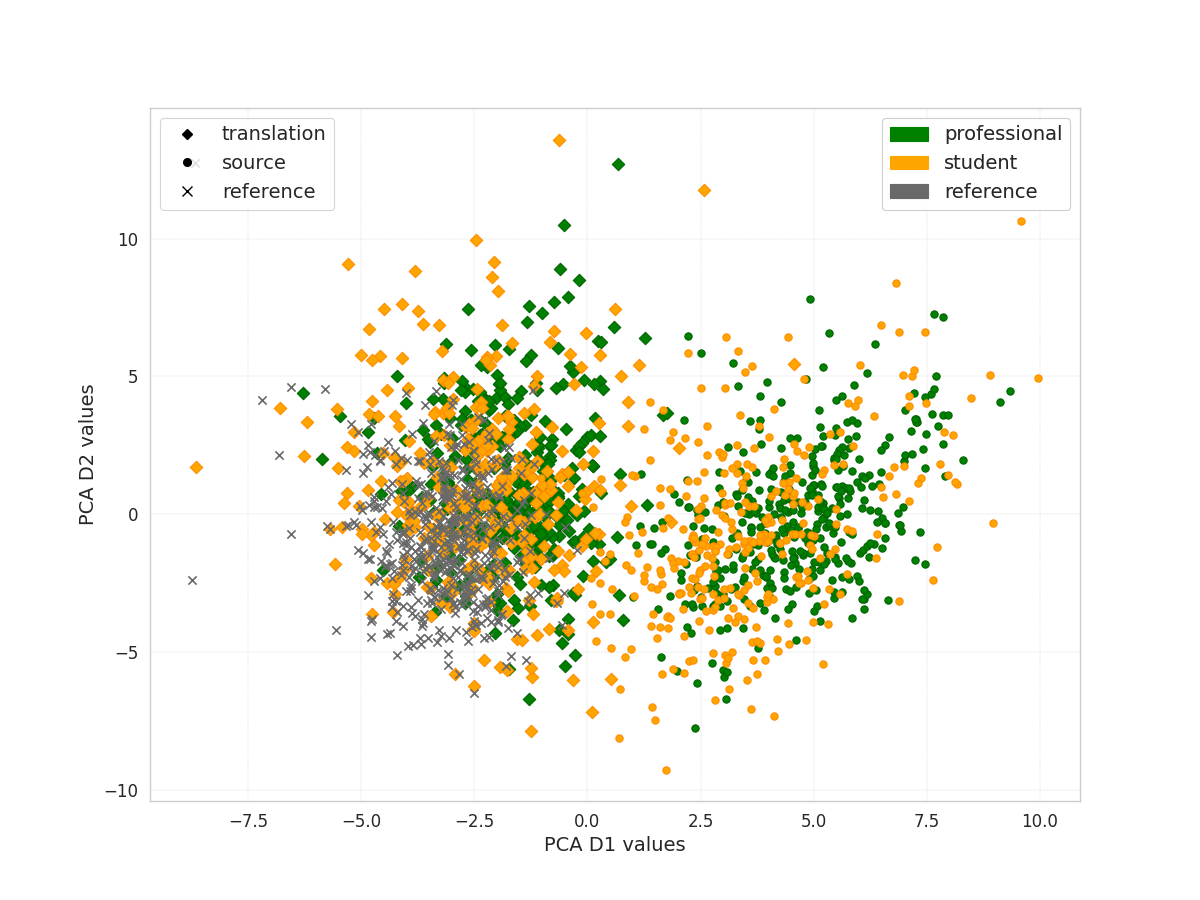
\includegraphics[width=\linewidth]{figures/pca/src-var-ttype-ud-PCA-scatter}
	\end{minipage}	
	\begin{minipage}[c]{0.5\linewidth}
		\centering
		Distribution along PCA D1
		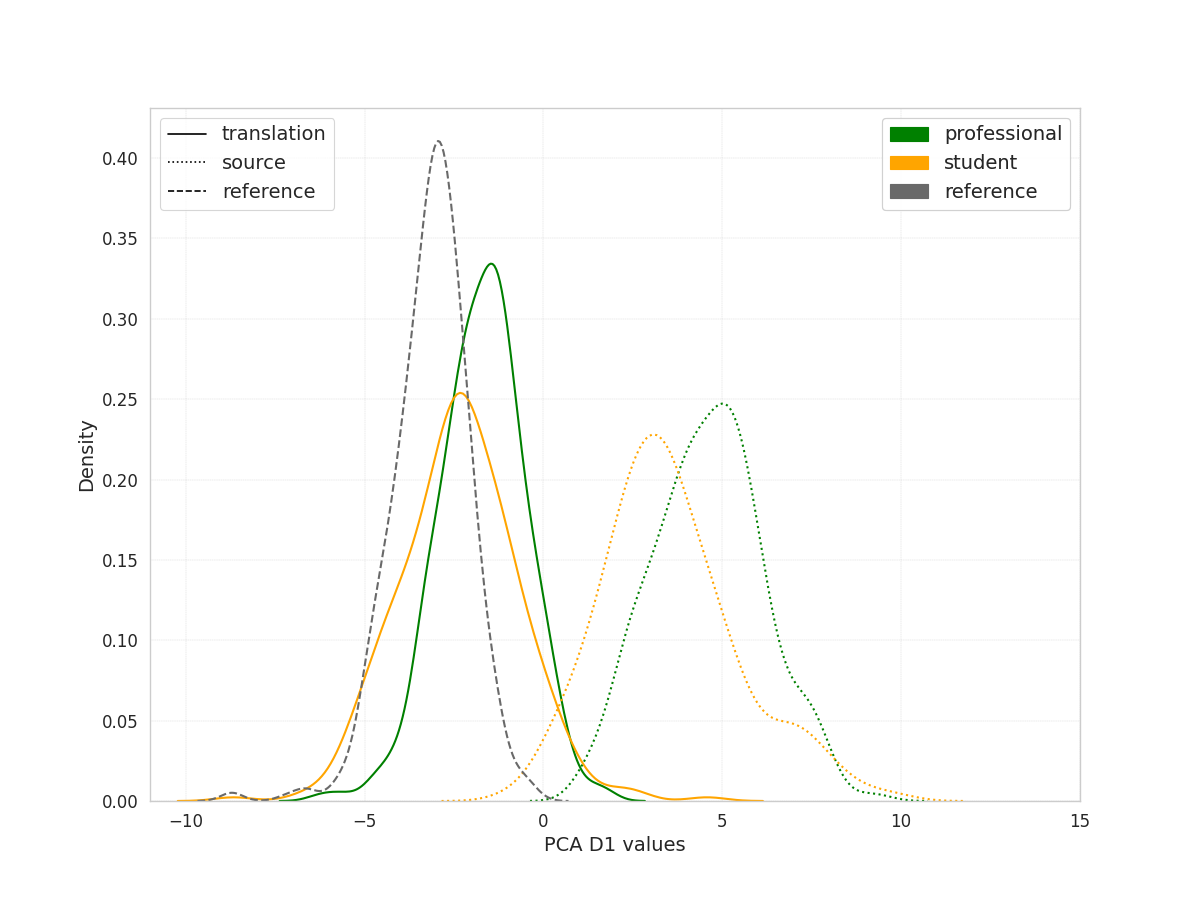
\includegraphics[width=\linewidth]{figures/pca/src-var-ttype-ud-PCA-D1-lines}
	\end{minipage}
	\caption{\label{fig:vars-ud}Visualisations of PCA transform based on \textit{UD} features}	
\end{figure}
  
Each marker represents a document from the respective colour-coded category. Coloured diamonds are used for translations, dots for source texts in English and dark grey crosses are non-translations in the TL. 
The most obvious distinction is between the two languages: Russian is on the left, English is on the right. 
It can be seen that most translations (coloured markers) are shifted to the right away from grey non-translations and towards source texts. 
The translation varieties are not clearly separated from non-translations and from each other. It means that the signal captured by fairly successful translationese classifications is distributed among the UD features and cannot be easily summarised by just two dimensions.
To be fair, PCA offers a very crude simplification for the underlying datasets. PCA D1 shown in Figure~\ref{fig:vars-ud} explains only 21\% of the total multivariate variability in the full UD dataset, with further 13\% captured on D2. 
Importantly, there is a visible difference in location between English source texts for professional and student translations: green dots of professional translation sources in left-hand panel in Figure~\ref{fig:vars-ud} seem to be further away to the right from the centre of the plot than orange dots of ST translated by students. ST is a known factor in shaping the properties of translations, and this difference should be taken into consideration in feature analysis. 

It can be argued that student translations (shown in orange) are the least compact cloud without a distinct location, while professional translations are a bit more homogeneous. This observation is supported by a more focused representation of document values on x-axis (PCA D1) in the right-hand panel of Figure~\ref{fig:vars-ud} using a kernel density estimation plot (a smoothened and scaled version of a histogram plot). The group of three line plots on the left shows the variation in distributions of PCA D1 values across the document classes in Russian. The shape of the flatter orange solid-line curve for student translations suggest more variability in the data. Both student and professional translations are shifted to the right from non-translations (grey dashed line) towards the area of English sources. It can be tentatively concluded that D1 captures language-contrast-related properties of documents, i.e. potential shining-through effect.
% UD Variance explained per dimension (if lose_src=False):  [0.21163434 0.13134273]
% UD Variance explained per dimension (if lose_src=True):  [0.16399743 0.13674201]

By way of comparison, consider the same types of visualisations for our best performing representation, namely, \textit{mdeberta3}, in Figure~\ref{fig:vars-deberta}. 

\begin{figure}[H]
	\begin{minipage}[c]{0.31\linewidth}
		\centering
		PCA	2D 
		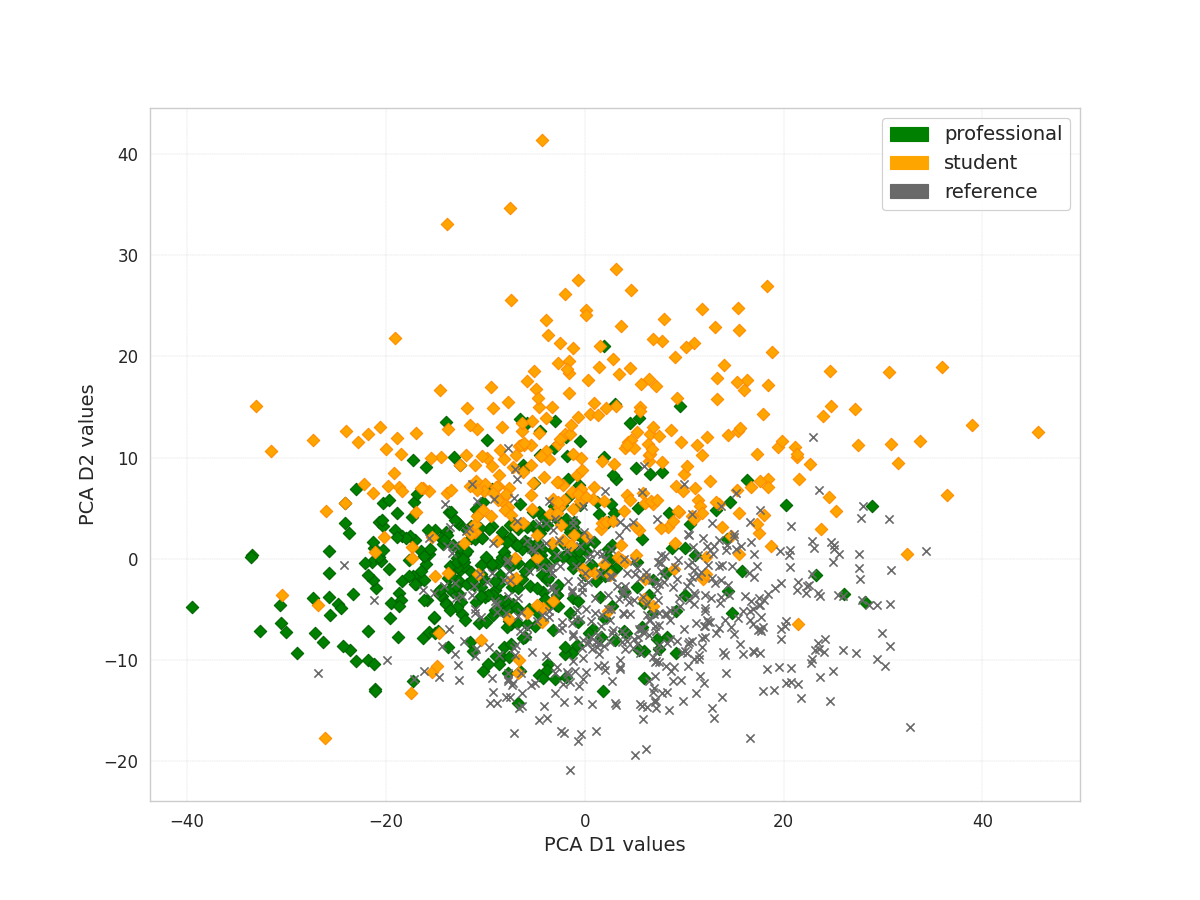
\includegraphics[width=\linewidth]{figures/pca/var-ttype-mdeberta3-base-PCA-scatter}
	\end{minipage}	
	\begin{minipage}[c]{0.31\linewidth}
		\centering
		PCA D1
		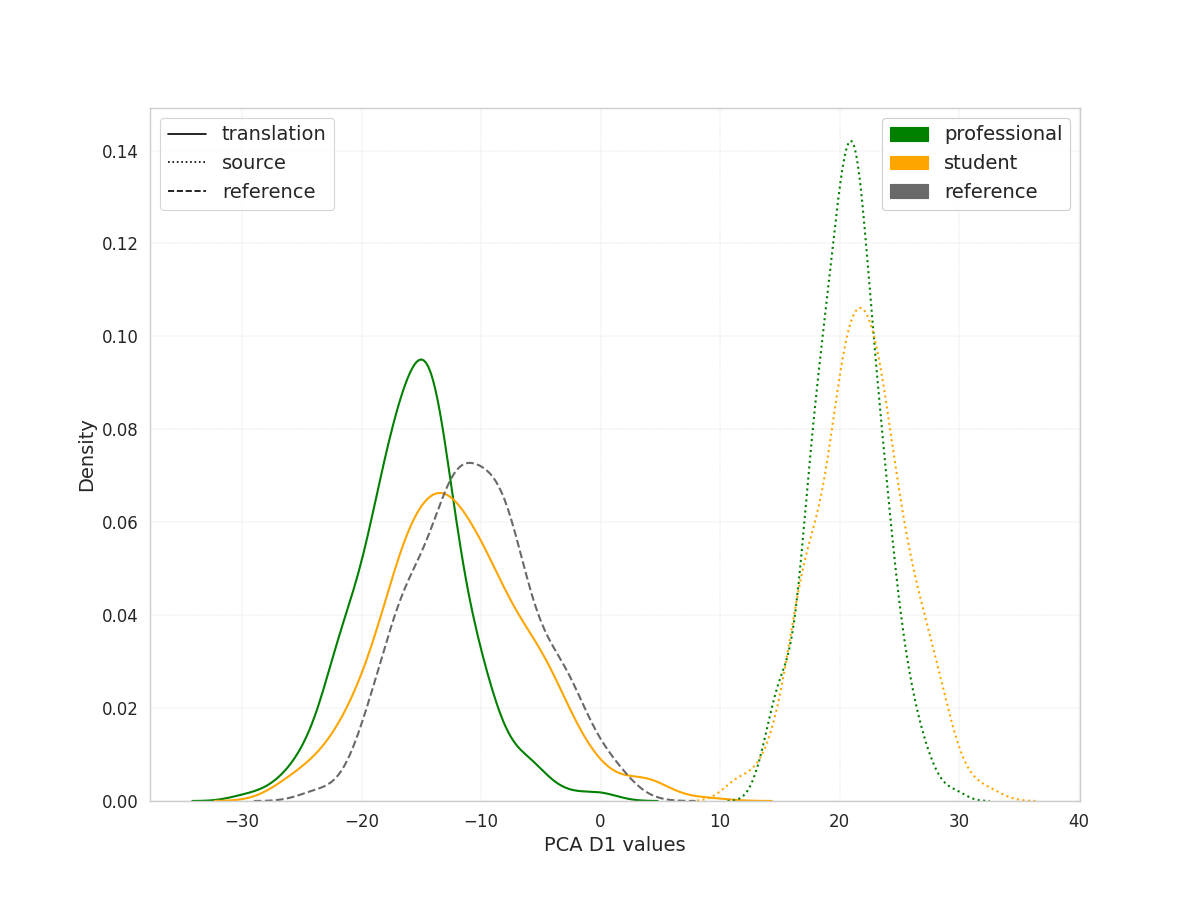
\includegraphics[width=\linewidth]{figures/pca/src-var-ttype-mdeberta3-base-PCA-D1-lines}
	\end{minipage}
	\begin{minipage}[c]{0.31\linewidth}
		\centering
		PCA D2
		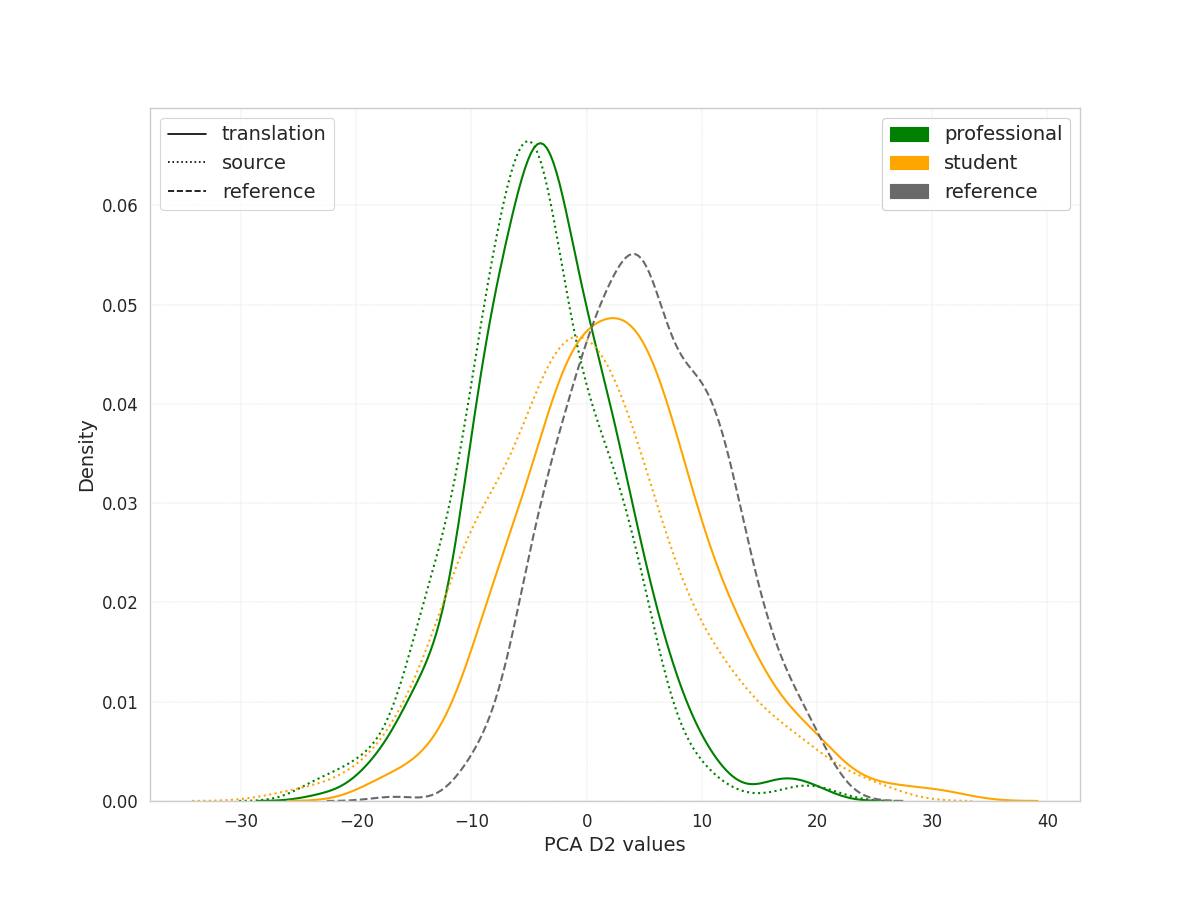
\includegraphics[width=\linewidth]{figures/pca/src-var-ttype-mdeberta3-base-PCA-D2-lines}
	\end{minipage}
	\caption{\label{fig:vars-deberta}Visualisations of PCA transform based on \textit{mdeberta3} representation}	
\end{figure}

If English sources are excluded from PCA analysis (they overshadow all other distinctions on multilingual vectors), the three classes of documents in the TL are more or less distinct and are located in different parts of the 2D scatter plot. D1 (x-axis) seems to capture the differences between professional translations and non-translations, while D2 (y-axis) values separate student translations from the other two categories. Unlike the previous representation, translations (regardless of professionalism level) were not grouped together against non-translations. If anything, student translations appear to have more in common with non-translations than with professional translations (see density plots in the middle and right-hand panels). It means that \textit{mdeberta3} did not really capture the commonalities of translations as an ontological text category. It is likely that the co-varying components of \textit{mdeberta3} vectors, aggregated by PCA, reflect semantic (topical) differences between categories along each of the axes. The right-most panel in Figure~\ref{fig:vars-deberta} suggests that student translation source texts are indeed semantically more similar to Russian non-translations than English source texts of professional translations. 
% mdeberta3 Variance explained per dimension (if lose_src=False):  [0.38012075 0.08784468]
% mdeberta3 Variance explained per dimension (if lose_src=True):  [0.21136208 0.09629121]

This impression is reproduced on \textit{stsb-xlm-r-m} vectors\wlvfootnote{\textit{Stsb-xlm-r-m} is a cross-lingual language model for many languages specifically trained to capture semantic similarities between sentences.} (see left-most panel in Figure~\ref{fig:other}). 
However, vectors from \textit{TQmono-m}, a Sentence Transformer fine-tuned on MT quality estimation task, when reduced by PCA, revealed the commonality between the two translation collections. Both student and professional translations demonstrate a shift away from non-translations in either language: solid coloured lines of translated documents are moved to the left from dotted and dashed lined of non-translations in the central panel in Figure~\ref{fig:other}. Interestingly, student translations are located further away from non-translated reference than professional translations, capturing the anticipated difference in the amount of translationese (see the central panel in Figure~\ref{fig:other}). 
Finally, the right-most scatter plot in Figure~\ref{fig:other} shows that a dedicated Russian contextualised word embedding model also detects translationese per se (and not the confounding topical differences between text categories): it separates all translations from non-translations, but this distinction is captured on a weaker D2 component (y-axis), while D1 probably captures the variation in topical content.   

\begin{figure}[H]
	\begin{minipage}[c]{0.31\linewidth}
	\centering
	stsb-xlm-r-m PCA D1 
	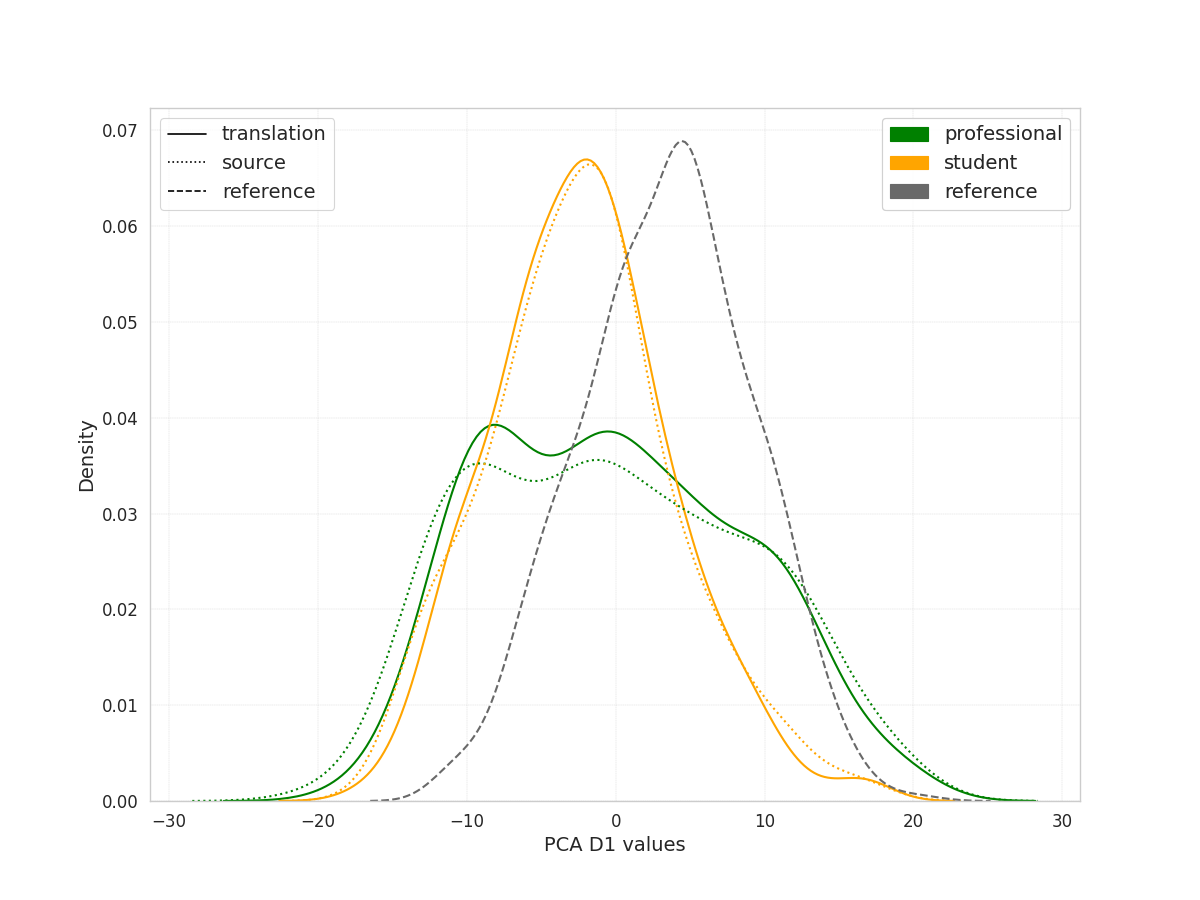
\includegraphics[width=\linewidth]{figures/pca/src-var-ttype-mXLM-R-PCA-D1-lines}
\end{minipage}	
\begin{minipage}[c]{0.31\linewidth}
	\centering
	TQmono-m PCA D1
	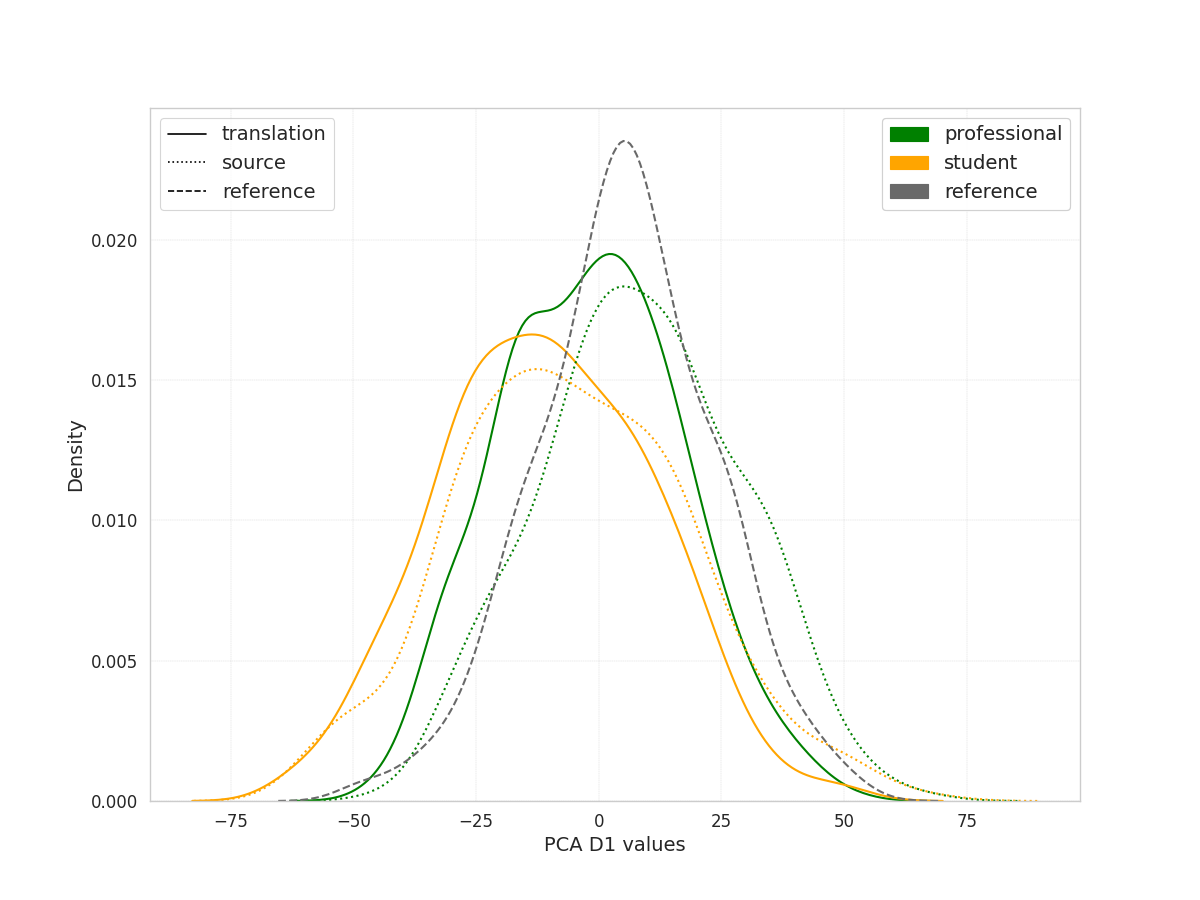
\includegraphics[width=\linewidth]{figures/pca/src-var-ttype-TQmono-m-PCA-D1-lines}
\end{minipage}
\begin{minipage}[c]{0.31\linewidth}
	\centering
	ruRoberta PCA 2D
	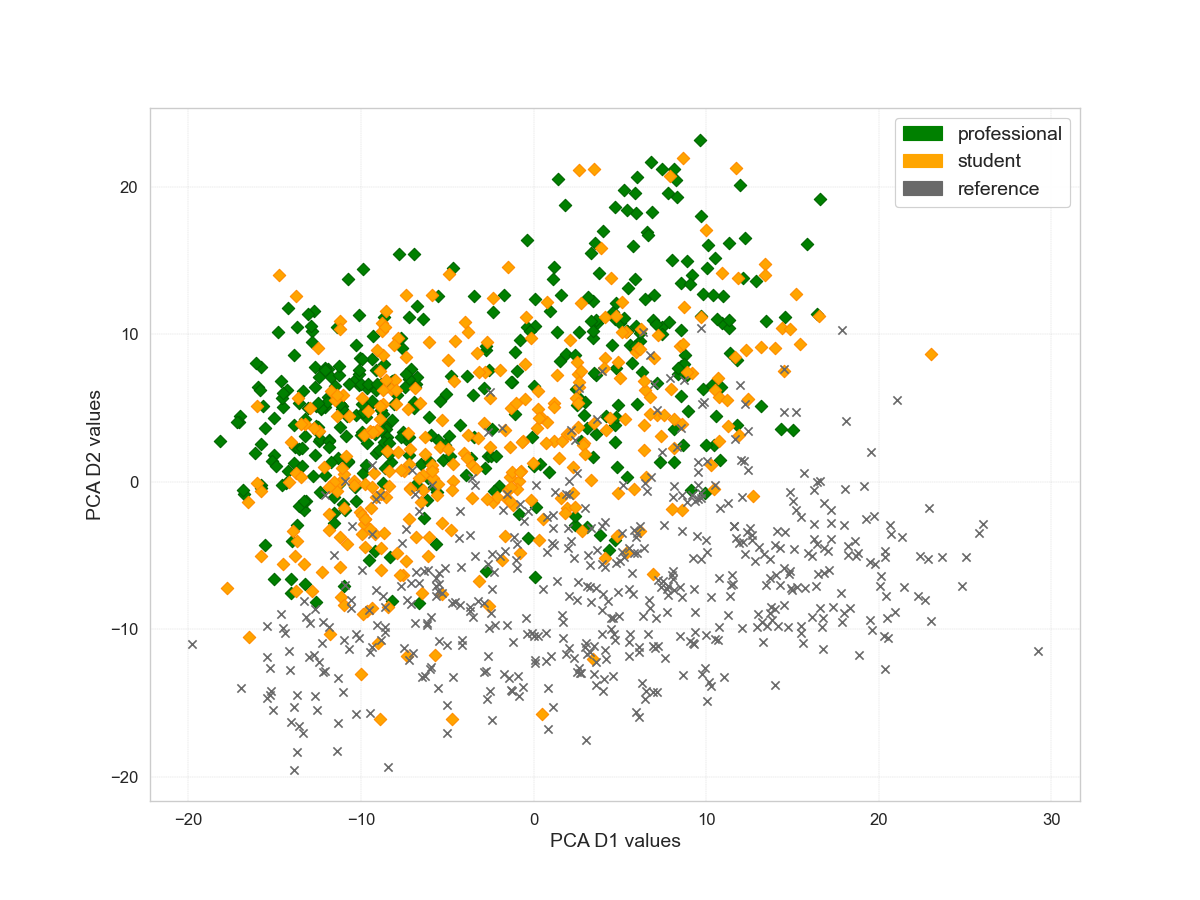
\includegraphics[width=\linewidth]{figures/pca/var-ttype-ruRoberta-large-PCA-scatter}
\end{minipage}
\caption{\label{fig:other}More informative aspects of PCA analysis on other contextualised embeddings}	
\end{figure}

% truth to be told, total variance captured by any dimentions in these representation in ridiculously small: 
%mXLM-R Variance explained per dimension:  [0.07467213 0.06423427]
%TQmono-m Variance explained per dimension:  [0.44481555 0.13820085]
%ruRoberta Variance explained per dimension:  [0.09490415 0.0667047 ] naturally no src

Despite contextualised embeddings seem to capture different aspects of documents relatedness, they achieved the same classification result: there were no significant differences between \textit{TQmono-m, ruRoberta and mdeberta3}, with \textit{stsb-xlm-r-m} being inferior only to \textit{ruRoberta} and \textit{mdeberta3} on professional translations by either SVM or neural classifier. 
On (more challenging) student translations mean-pooled word embeddings (\textit{ruRoberta} and \textit{mdeberta3}) significantly outperformed both sentence embedding models (\textit{TQmono-m} and \textit{stsb-xlm-r-m}) at least by SVM.
% By neural classifier TQmono-m is not different from word-embeddings, while stsb-xlm-r-m significantly loses to all of them

The next section describes UD features from the point of view of their usefulness for translation detection. It reports the results of feature selection, based on SVM feature weights and describes univariate comparisons between text categories to reveal most important translationese indicators as well as trends that these indicators contribute to. This analysis is necessary to interpret the results of professionalism- and quality-related classifications in Chapter~\ref{cha:pro_qua} with regard to our main hypothesis that translationese indicators can be related to translation quality.

\section{\label{sec:bestof}Feature Analysis}
This section presents the results of feature analysis, which detects strong translationese predictors among the manually engineered features, and provides a linguistic description of translationese in English-to-Russian language pair.
The primary method to achieve this goal is feature selection, supported by univariate feature analysis and statistical significance tests.

%Eventually, we want to see whether strong translationese indicators are correlated with professionalism and quality labels/scores and could predict them in a ML setup. 

\subsection{\label{ssec:best_ud}Best of UD features}

\paragraph{\label{par:detect_select}Feature selection}
As discussed above (see page~\pageref{par:featanal_meths}), \gls{RFECV} was preferred over \gls{ANOVA} for feature selection because many UD features did not meet the ANOVA requirement of normal distribution and equal variances across compared text categories. In contrast, RFECV relies on internal SVM feature weights and gradually prunes less useful ones to reduce the feature set to the best N features. 
%To infer N experimentally instead of using an arbitrary number, RFE was run in a cross-validation setup (RFECV). In our experiments, the algorithm iterated N in the range [3 : size of the feature set], performed 5-fold cross-validation on each N and returned N with the highest mean F1-score across all folds.

%RFECV: Shared best UD features for translation detection (28):
%{'addit', 'ppron', 'nnargs', 'compar', 'attrib', 'nsubj', 'sconj', 'pverbals', 'fixed', 'mark', 'determ', 'finites', 'wdlength', 'acl', 'advmod', 'deverbals', 'acl:relcl', 'copula', 'aux:pass', 'obj', 'amod', 'simple', 'pasttense', 'neg', 'ccomp', 'nmod', 'sentlength', 'advcl'}

% 'deverbals' was #33 that was not reflected in the symmetric weights graph
Feature selection on UD feature set returned $N=33$ and $N=42$ for translationese classifications on professional and student translations, respectively. 
After discarding noisy and collinear features, the performance of both classification improved. It went up by 1.3 percentage points from 90.22 to 92.04\% for professional translations, and by 2.1 percentage points from 88.96 to 91.06\% for student translations (based on F1-scores). % the statistical differences were not significant in either case on the results of 10 runs in cross-validation setup (on either ttest and on WMW U test, yes, we tried both just in case).

Figures~\ref{fig:pro-weights} and~\ref{fig:stu-weights} visualise the weights assigned to the respective subsets of best features in each classification. Features with larger absolute weights can be considered more predictive of the distinctions between categories. 
Detailed explanations of shorthand used on the x-axis can be found in Appendix~\ref{appx:ud}.
\vspace{-2em}
\begin{figure}[H]
	\centering
	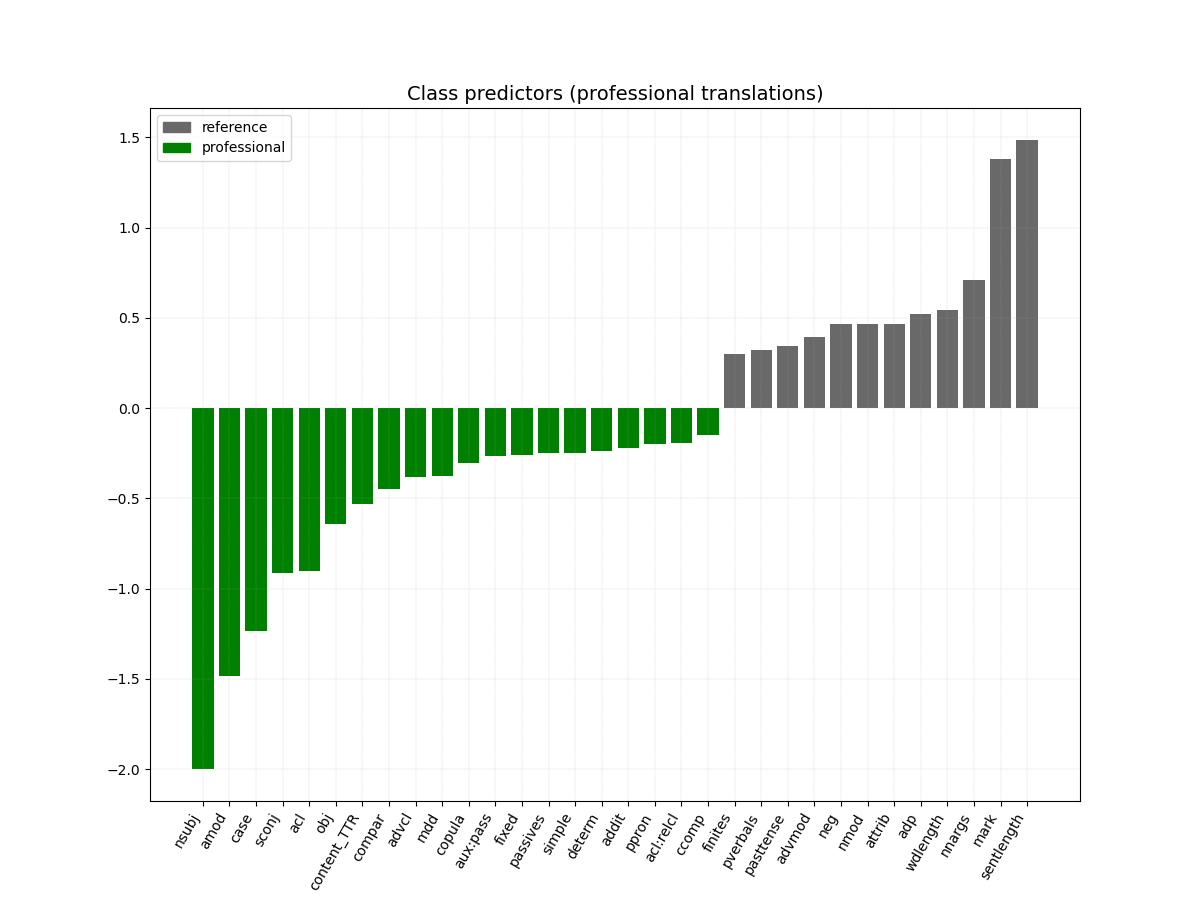
\includegraphics[width=.80\linewidth]{figures/pro-ref-bars-ud33}
	\caption{\label{fig:pro-weights}Weights loading the decision towards each category for 32 RFECV-selected items}	
\end{figure}
\vspace{-2.5em}
\begin{figure}[H]
	\centering
	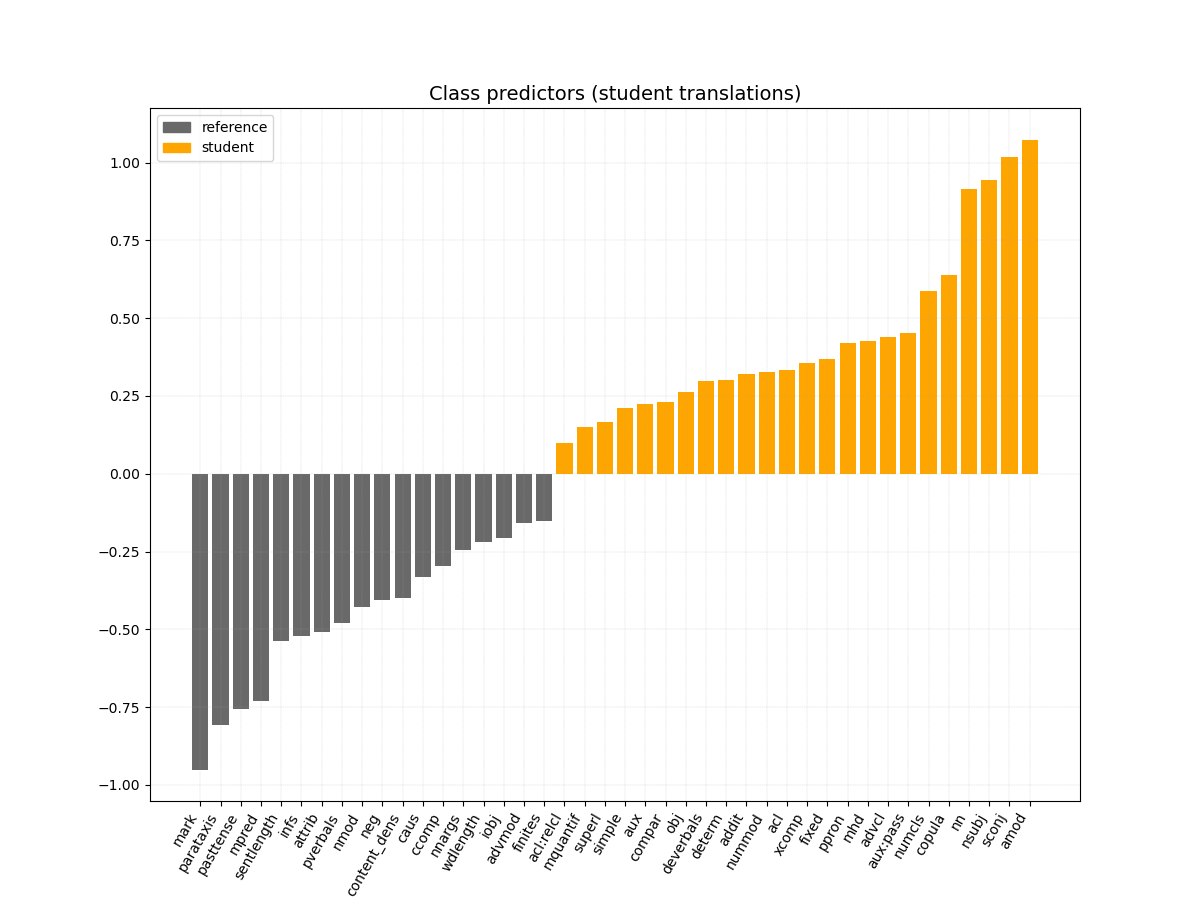
\includegraphics[width=.80\linewidth]{figures/stu-ref-bars-ud42}
	\caption{\label{fig:stu-weights}Weights loading the decision towards each category for 42 RFECV-selected items}	
\end{figure}
\vspace{-2.5em}

%RFECV: Shared best UD features for translation detection (28, sorted by average absolute weight): nsubj, amod, mark, sentlength, sconj, acl, pasttense, attrib, nnargs, copula, obj, nmod, neg, advcl, pverbals, wdlength, aux:pass, compar, fixed, ppron, advmod, addit, determ, deverbals, simple, finites, ccomp, acl:relcl
To have a closer look at the commonalities between translation varieties and feature importance in these selections, the lists were intersected and ranked based on the weights assigned by the linear kernel SVM algorithm. Feature weights were obtained from classifiers run on full datasets (without reserving a fraction for testing). Experiments showed that the feature weights were approximately the same if the weights were averaged across the models learnt on each of the folds in a cross-validation setup.

There were 28 UD features shared between the optimal sets of 33 and 42 translationese indicators in professional and student translationese classifications, respectively. They can be considered strong predictors that capture translational specificity regardless the level of expertise.
The full list of features includes: \textit{amod, sconj, mark, nsubj, pasttense, copula, sentlength, attrib, pverbals, aux:pass, advcl, nmod, ppron, neg, fixed, acl, addit, determ, deverbals, ccomp, obj, nnargs, compar, wdlength, simple, advmod, finites, acl:relcl}.\wlvfootnote{Because the weights for a feature could be quite diverging in professional and student classifications (Spearman correlation was 0.47), the features on this list appear in the descending order according to the absolute weights in the student classification, a hypothetical marked quality class in this research.} 
These features are shown as either `translation predictors' (coloured bars in Figures~\ref{fig:pro-weights} and~\ref{fig:stu-weights}) or `non-translation predictors' (grey bars). Although the weights are shown as loading towards a specific category (reference or translations), it is not clear how this choice is made by the algorithm and this aspect is ignored in our analysis. 
%We were not able to detect any patterns in the data that would explain why some features were weighted to predict translations and others -- non-translations. 

Below we present these 28 features in two typological groups. Two-thirds of the shared features reflected various aspects of sentence structure, rather than frequencies of morphological units. Translationese-related syntactic phenomena were: 
% syntax: amod, mark, nsubj, copula, sentlength, attrib, pverbals, deverbals, advcl, finites, nmod, neg, acl, addit,  ccomp, obj, simple, advmod,  acl:relcl
\begin{description}\compresslist{}
	\item[nsubj, obj:] distribution of core verbal arguments (nominal subjects and objects),
	\item[mark:] frequency of function words that identify another word as a head of a subordinate clause,
	\item[acl:relcl, advcl, acl, ccomp:] frequencies of relative and adverbial clauses, finite and non-finite clauses that modify a nominal or function as clausal complements,  % the issues as he sees them, years to come
	\item[finites, pverbals:] closely related to the previous features, the distributions of finite and non-finite verbal forms in adverbial function, including Russian-specific verb form referred to as a converb (\textcyrillic{\textit{деепричастие}}), a type of participle in the adverbial function,
	\item[deverbals:] ratio of de-verbal nouns, naming of processes, actions, states, to the number of verbs,
	\item[amod, attrib, nmod:] modifiers of noun, including adjectives, participles and other nouns in attributive function (e.g. genitive complement: \textcyrillic{\textit{времена (финансовой) стабильности}} [times of (financial) stability], \textcyrillic{\textit{список грехов}} [list of sins]),
	\item[advmod:] non-clausal adverbial modifier (e.g. \textcyrillic{\textit{но и для выражения сочувствия}} [but also for offering condolences], \textcyrillic{\textit{N существует в виде статичных изображений}} [N exists in static images]),
	\item[simple:] proportion of simple sentences to all sentences in a document, 
	\item[sentlength:] average number of words in a sentence, care was taken to exclude pseudo-sentences that had only numbers and punctuation marks, or contained less than two tokens,
	\item[copula:] function words linking subject to a non-verbal predicate, 
	\item[neg:] negative particles or main sentence negation,
	\item[addit:] additive conjunctions of parenthetical type (such as \textit{what's more, in other words, furthermore, in this regard}), which are optional elements, external to the sentence structure.
\end{description}
Morphological classes, categories and forms, whose quantitative parameters were useful for translation detection, included: 
% morph: sconj, pasttense, aux:pass, ppron, fixed, determ, nnargs, compar, wdlength, 
\begin{description}\compresslist{}
	\item[nnargs:] ratio of nouns or proper names as verb arguments to total of respective functions,
	\item[ppron:] personal pronouns, excluding possessive pronouns,
	\item[sconj:] subordinative conjunctions,
	\item[aux:pass:] analytical passive verb forms
	\item[pasttense:] verbs in past tense,
	\item[fixed:] fixed \gls{MWE}, mostly functional words (e.g. \textcyrillic{\textit{то есть}} [that is]; \textcyrillic{\textit{до сих пор}} [until now]),
	\item[determ:] pronominal determiners (e.g. \textcyrillic{\textit{кaждый}} [every], \textcyrillic{\textit{этот}} [this]),
	\item[compar:] comparative degree of comparison for adjectives and adverbs,
	\item[wdlength:] average number of characters in content words only to avoid co-linearity with features counting various function words.
\end{description}

There were five features that were specific for professional (but not student) translation classification: \textit{adp, passives, mdd, case, content\_TTR}. 
%	\item[case:] function of any syntactic word functioning as case marker (e.g. \textcyrillic{\textit{для полиции; за меньшие деньги}} [for police, for less money]).

To achieve the best result in predicting student translations, SVM considered distributions of 14 more features that were not selected in the classification based on professional translations: \textit{numcls, parataxis, mpred, xcomp, aux, content\_dens, superl, nummod, mhd, iobj, nn, mquantif, infs, caus}. 

Features that were not selected by RFECV for either professional-vs-non-translation or student-vs-non-translations classifications included 13 items. They can be considered less useful for translation detection either due to the lack of considerable distinctions between the categories or due to collinearity with other features. This list had values for the following features:
%Not selected by RFECV for either pro-ref or stu-ref (13): obl, appos, advers, cconj, discourse, epist, possp, tempseq, flat, anysome, compound, interrog, conj
\begin{description}\compresslist{}\label{pg:rfe_useless}
	\item[tempseq:] cumulative frequency of temporal and sequential connectives (e.g. \textcyrillic{\textit{короче говоря}} [to put it briefly], \textcyrillic{\textit{в конце концов}} [finally, in the end]),
	\item[discourse:] a dependency relation for interjections and other discourse particles (e.g. \textcyrillic{\textit{в первую очередь}} [in the first place], \textcyrillic{\textit{в частности}} [in particular]),
	\item[epist:] epistemic markers of author's stance (e.g. \textcyrillic{\textit{навряд ли}} [unlikely], \textcyrillic{\textit{можно не сомневаться}} [no doubt], \textcyrillic{\textit{вероятно, наверняка}} [probably, definitely]),
	\item[possp:] possessive pronouns,
	\item[cconj, conj:] frequencies of coordinating conjunctions and respective syntactic relation between two conjuncts, 
	\item[advers:] adversative (contrastive) discourse markers (e.g. \textcyrillic{\textit{впрочем}} [however], \textcyrillic{\textit{несмотря на, тем не менее}} [despite, nevertheless])
	\item lexical density, counted as ratio of PoS disambiguated content word types to all tokens,
	\item simple sentences,
	% (e.g. \textcyrillic{\textit{}} [])
	\item[flat, compound:] two types of \gls{MWE}: exocentric semi-fixed sequences such as proper names and dates (e.g. \textcyrillic{\textit{Синдзо Абэ; 24 декабря}} [Shinzo Abe, 24 December]) and endocentric compound MWE, usually hyphenated in Russian (e.g. \textcyrillic{\textit{черно-белый}} [black and white]),
	\item[amod:] non-clausal adjectives and participles functioning as attributes (e.g. \textcyrillic{\textit{финансовый центр}} [financial centre]), % mostly adjectives and participles functioning as attributes, but also "nothing wrong with it", e.g. , удобный гаджет
	\item[obl:] frequency of non-core verbal arguments expressed by a noun (e.g. indirect objects),
	\item[appos:] punctuated or parenthetical modifiers of noun (e.g. \textcyrillic{\textit{мы, демократы}} [we, the democrats], \textcyrillic{\textit{мисс Пигги, персонаж Маппет-шоу}} [miss Piggy, a Mappet show character]),
	\item[interrog:] proportion of sentences ending in question mark,
	\item[anysome:] indefinite and total pronouns (e.g. \textcyrillic{\textit{кому-нибудь, чем-то, когда-то}} [anyone, something, at some point]),

\end{description}

All features on the list above had weak association with the labels (F1-score 0.36 to 0.46), with the exception of oblique nominal objects (\textit{obl}), a non-core verbal argument introduced in Russian by a preposition and, therefore collinear with the frequency of prepositions. Some features on this list seem to disprove a common anticipation by the translation textbooks of deviant use of respective items in translation. However, their use in `translationese' contexts might have been subsumed by other more natural contexts. For example, the use of pronouns, including possessive and indefinite/total, is expected to be different under the pressure of the ST. Although this analysis failed to find empiric proof for that, we will be weary of dismissing pronouns as a translationese give-away. It is likely that this feature requires taking into account translation-specific contexts to reveal its potential as a translationese indicator.      

The next paragraph explores the distributional properties of the best translationese indicators revealed in the feature selection process across document categories (translations, sources and non-translations). This contrastive-comparative univariate analysis helps to group features according to specific trends in translational behaviour as reflected by linguistic properties of translated documents. 

\paragraph{\label{par:featsunivar}Univariate analyses}
To understand more about the prominent patterns of language use in translations picked up by SVM classifiers, we performed a series of statistical tests on individual features identified as strong translationese indicators in the previous paragraph. This procedure aims at revealing the impact of the language pair on the linguistic properties of translations.\wlvfootnote{The distance between the languages is not the only factor that affects translational behaviour, but we do not have the necessary setup to measure the possible contribution from those other factors.} 
 
For each feature, we compared its distributions in sources, targets and non-translations. The differences were tested for statistical significance using \textit{Mann-Whitney U test for independent samples} and \textit{Wilcoxon signed-rank test} for paired samples of source and target texts. 

\begin{longtable}[H]{l|l|p{3cm}p{8cm}}
	\toprule		
	& group & trend & description \\
	\midrule
	\parbox[t]{2mm}{\multirow{20}{*}{\rotatebox[origin=c]{90}{high ------------ amount of effort ------------ low}}}	&	\multirow{3}{*}{reproducing ST}& anglicisation (ref<src<tgt)& TT values greater than in SL and much greater than in TL, possibly the use of SL patterns even when unprompted \\
	\cmidrule{3-4}
	% ref<src=tgt
	&	& shining-through ref<tgt=src & No difference between ST and TT values, both are higher than in TL \\
	\cmidrule{3-4}
	&	& overuse of SL ref<tgt<src & Many translation decisions are prompted by ST, which has higher values than in TL \\
	\cmidrule{2-4}
	&	\multirow{4}{*}{counteracting ST} &  underuse of TL tgt<=src<ref & Lack of effort to add typical TL items when not prompted by ST \\
	\cmidrule{3-4}
	&	& normalisation src<=tgt<ref & Insufficient efforts to bring ST frequencies in line with TL norm \\
	\cmidrule{3-4}
	&	& russification src<ref<tgt tgt<ref<src & Active use of TL patterns unseen in ST or effective counteraction of ST influence leading to more expressed TL patterns \\ %(overuse of specific items or lack of less typical TL items)
	\cmidrule{3-4}
	&	& adaptation tgt=ref<src src<ref=tgt & No translationese: significant differences between the two languages are reconciled in favour of the TL norm \\
	\cmidrule{2-4}
	& third code & SL/TL-independent tgt<ref=src ref=src<tgt & Translationese features with significant differences from both languages and no language gap \\
	\bottomrule
	\caption{\label{tab:trends}Patterns in translational behaviour (SL=source language, ST=source text, TL=target language, TT=target text)}\\
\end{longtable}

First, we identified the features that had significant differences between translations and non-translations (\textit{tgt} and \textit{ref} categories): these are translationese indicators by definition. 
Then, we established whether there were statistically significant differences between the two languages (\textit{src} and \textit{ref} categories) with respect to a given feature, and which language had greater values.
Finally, for each feature, we performed pairwise comparisons between frequencies in translations and in each of the languages.

The outcome of the above sequence of tests can be viewed as capturing the amount of effort invested by a translator to reconcile differences between the two languages (if any) for a given feature. The features, representing various trends in translational behaviour, can be arranged in three major groups (see Table~\ref{tab:trends}), depending on the adopted translation strategy and the scale of its implementation. 

There was a group of features that were useless for a translationese study, because they had the same frequencies in translations and non-translations, and also did not distinguish the languages. In the classification based on professional translations, this group included frequencies of adpositions (prepositions) and discourse particles such as interjections. In student translation data, there were no statistically significant differences between document categories for interrogative sentences and adverbial quantifiers (e.g. \textcyrillic{\textit{совершенно}} [entirely],  \textcyrillic{\textit{чрезмерно}} [utterly]).

Further on, we established the strength of association between each feature values and binary categorical labels (translation, non-translation) by measuring the quality of single-feature logistic regression classifier using macro F1-score (LogR F1). The results of significance tests and variable-label association analysis are collected in Table~\ref{tab:shared_rfecv_feats}. The features selected by RFECV are sorted by LogR F1-score averaged for students and professionals. Statistically significant results are indicated by \textit{less-than} and \textit{greater-than} signs, the lack thereof is shown with an \textit{equals} sign.

%in a similar recent study \cite{Hu2021} reached an accuracy of 96.55\% on 160 cohesive markers alone
%how discriminative these characteristics are?
% does a feature typify O or T according to a log-likelihood (LL)? I need raw counts for that, I have only normalised frequencies, some values are not freqs at all!
\begin{longtable}[H]{p{1.6cm}|ccc||ccc}
	\toprule
		      &      \multicolumn{3}{c}{Professional} 	&      \multicolumn{3}{c}{Student}\\
	\midrule
	feature & LogR F1 & trend & means   & LogR F1 & trend   & means   \\
	\midrule
	nsubj   & \textbf{0.82} & overuse of SL  & ref\textless{}tgt\textless{}src & \textbf{0.71} & shining & ref\textless{}tgt=src  \\
	mark & \textbf{0.74} & overuse of SL  & ref\textless{}tgt\textless{}src & \textbf{0.68} & overuse of SL & ref\textless{}tgt\textless{}src \\
	acl:relcl  & \textbf{0.69} & overuse of SL  & ref\textless{}tgt\textless{}src & \textbf{0.66} & overuse of SL & ref\textless{}tgt\textless{}src \\
	advcl   & \textbf{0.7}  & overuse of SL  & ref\textless{}tgt\textless{}src & \textbf{0.63} & overuse of SL & ref\textless{}tgt\textless{}src \\
	obj  & \textbf{0.72} & overuse of SL  & ref\textless{}tgt\textless{}src & \textbf{0.61} & overuse of SL & ref\textless{}tgt\textless{}src \\
	fixed   & \textbf{0.56} & russification  & src\textless{}ref\textless{}tgt & \textbf{0.58} & russification & src\textless{}ref\textless{}tgt \\
	sentlength & \textbf{0.61} & NA  & ref\textless{}tgt & \textbf{0.57} & NA & ref\textless{}tgt \\
	acl  & \textbf{0.62} & shining  & ref\textless{}src=tgt  & \textbf{0.56} & shining & ref\textless{}src=tgt  \\
	nnargs  & \textbf{0.68} & normalisation  & src\textless{}tgt\textless{}ref & \textbf{0.55} & normalisation & src\textless{}tgt\textless{}ref \\
	amod & \textbf{0.51} & russification  & src\textless{}ref\textless{}tgt & \textbf{0.53} & russification & src\textless{}ref\textless{}tgt \\
	attrib  & \textbf{0.51} & russification  & src\textless{}ref\textless{}tgt & \textbf{0.52} & russification & src\textless{}ref\textless{}tgt \\
	copula  & \textbf{0.52} & overuse of SL  & ref\textless{}tgt\textless{}src & \textbf{0.51} & overuse of SL & ref\textless{}tgt\textless{}src \\
	ccomp   & \textbf{0.63} & overuse of SL  & ref\textless{}tgt\textless{}src & \textbf{0.5}  & overuse of SL & ref\textless{}tgt\textless{}src \\
	nmod & 0.36 & adaptation  & src\textless{}ref=tgt  & \textbf{0.5}  & russification & src\textless{}ref\textless{}tgt \\
	deverbals  & 0.45 & normalisation  & src\textless{}tgt\textless{}ref & 0.45 & russification & src\textless{}ref\textless{}tgt \\
	addit   & 0.4  & shining  & ref\textless{}src=tgt  & 0.43 & SL/TL-indep   & ref=src\textless{}tgt  \\
	wdlength   & 0.4  & NA  & tgt\textless{}ref & 0.43 & NA & ref\textless{}tgt \\
	pasttense  & \textbf{0.51} & SL/TL-indep & tgt\textless{}ref=src  & 0.42 & SL/TL-indep   & tgt\textless{}ref=src  \\
	neg  & 0.41 & normalisation  & src\textless{}tgt\textless{}ref & 0.4  & normalisation & src\textless{}tgt\textless{}ref \\
	advmod  & \textbf{0.53} & overuse of SL  & ref\textless{}tgt\textless{}src & 0.38 & SL/TL-indep   & tgt\textless{}ref=src  \\
	aux:pass   & 0.36 & russification  & tgt\textless{}ref\textless{}src & 0.38 & adaptation & tgt=ref\textless{}src  \\
	compar  & 0.38 & overuse of SL  & ref\textless{}tgt\textless{}src & 0.38 & overuse of SL & ref\textless{}tgt\textless{}src \\
	finites & 0.36 & adaptation  & tgt=ref\textless{}src  & 0.38 & overuse of SL & ref\textless{}tgt\textless{}src \\
	determ  & 0.36 & overuse of SL  & ref\textless{}tgt\textless{}src & 0.37 & overuse of SL & ref\textless{}tgt\textless{}src \\
	ppron   & 0.36 & overuse of SL  & ref\textless{}tgt\textless{}src & 0.37 & overuse of SL & ref\textless{}tgt\textless{}src \\
	pverbals   & 0.36 & adaptation  & src\textless{}ref=tgt  & 0.37 & adaptation & src\textless{}ref=tgt  \\
	sconj   & 0.36 & russification  & src\textless{}ref\textless{}tgt & 0.37 & russification & src\textless{}ref\textless{}tgt \\
	simple  & \textbf{0.67} & underuse of TL & tgt\textless{}src\textless{}ref & 0.37 & underuse of TL & tgt\textless{}ref\textless{}src \\
	\bottomrule
	\caption{\label{tab:shared_rfecv_feats}Patterns of translational behaviour with regard to 28 UD features selected as a best-performing subset in translations vs non-translations classifications by RFECV (NA is used for features, where cross-linguistic comparisons are problematic due to typological differences)}\\
\end{longtable}
With regard to the strength of association between feature values and class labels (translations, non-translations), only half of shared features from RFECV selections yield F1-scores above the chance level (0.5) when used in a single-feature classifier. Their values are shown in bold in Table~\ref{tab:shared_rfecv_feats}.

Table~\ref{tab:shared_rfecv_feats} indicates that the more salient deviations from non-translation for both translation varieties can be described by the same trends. Half of translationese indicators in both translation collections pointed that translators \textbf{reproduced patterns observed in the SL} (overuse of SL patterns, shining-through or anglicisation). They had frequencies, which were shifted towards SL value and were higher than expected in the TL. For example, the overuse of SL patterns was seen for \textit{nsubj, mark, acl:relcl, advcl, obj}. Another translational trend is associated with features, where translators actively \textbf{counteracted the influence of the ST and brought the frequencies in translations closer to the TL norm}. Underuse of TL items, normalisation, russification and adaptation together explained 13 (professionals) and 12 (students) out of 28 translationese indicators. A few features can be described as contributing to \textbf{SL/TL-independent translationese} (e.g \textit{pasttense} and \textit{advmod, addit} in student translations). This group represents the trends in translational behaviour that were likely to be brought about by factors other than SL/TL contrast. 

For some features, sources and TL reference compare differently in professional and student translations. It may or may not result in changes in their interpretation with regard to investigated translational trends. 
For example, both professionals and students generated fewer simple sentences than can be expected in the TL. However, professional translators faced a much more challenging situation: their sources had fewer simple sentences than in the TL to start with. Students, on the contrary, did not have to overcome the pressure of the ST as their sources had more simple sentences than in the TL. Nonetheless, students demonstrated a known translational behaviour to use longer sentences with multiple clauses and converted the surplus of simple sentences into the lack of thereof with regard to the TL norm. 
% pro simple : src 0.29 +/-0.10  tgt 0.23 +/-0.09  ref 0.31 +/-0.10
% stu simple : src 0.34 +/-0.14  tgt 0.29 +/-0.13  ref 0.31 +/-0.10

The case of additive discourse markers (\textit{addit}) is another example of how ST properties can impact the outcomes of this analysis. Professionals seem to have carried over the additive markers that were seen in the source texts, while students' behaviour was indeed divergent from both ST and TL: students generated surplus additive markers where they were not seen in sources. Overuse of overt linking parentheticals is a known problem of novice writers and translators, who rely on `crude force', using external markers of cohesion instead of making efforts towards a better sentence structure.  
%pro addit: ref<src=tgt src 0.09 +/-0.06 tgt 0.09 +/-0.07 ref 0.08 +/-0.06
%stu addit: ref=src<tgt src 0.08 +/-0.09 tgt 0.10 +/-0.09 ref 0.08 +/-0.06

The anticipated outcome of this analysis is seen for analytical passives (\textit{aux:pass}). Both students and professionals avoided carrying over English passive form, which had a corresponding form in Russian. Both professionals and students made efforts to replace English analytical passives with either of the other three Russian forms to express passive relations as can be seen from the frequencies for overall counts for passive forms (see \textit{passives} in Table~\ref{tab:spec_rfecv_feats}). However, professionals viewed the legitimate isomorphic Russian form as less acceptable, which led to the lack of analytical passives in their Russian translations (as compared to non-translations). Interestingly, textbooks on practical translations from English into Russian tend to emphasise English passives as a typical source of less fluent translationese solutions. Some authors made it appear that there were more passive constructions in English than in Russian~\cite[see, for example,][]{Zrazhevskaya1972, Belyaev2010, Borisova2019}. We have seen, however, that it is only true for analytical passives.
% I have a lot of examples for analytical passives avoided in professional translations in "not analytical passives in prof translations" note in Nixnote.

The strength of association for most features is higher for professional than for student translations. We attribute this to structural simplicity of the source texts offered to students, on the one hand, and to the difference in the size of the underlying subcorpora, on the other. As demonstrated in Table~\ref{tab:corpus_means}, student translations had fewer instances, the smallest mean document length in tokens and in number of sentences, and at the same time, the largest STD for both parameters. Smaller corpus size could have contributed to the sparsity of investigated features.

\begin{table}[H]
	\begin{tabular}{l|llll}
			\toprule
			subcorpus                 & docs & tokens per doc   & tokens per sent & sent per doc  \\
			\midrule
			student translations      & 334  & 646.88 (+/-984.07)  & 22.39 (+/-4.81)    & 29.68 (+/-40.68) \\
			professional translations & 404  & 950.45 (+/-282.42)  & 22.95 (+/-4.03)    & 42.44 (+/-13.42) \\
			non-translations          & 497  & 1053.80 (+/-539.18) & 20.48 (+/-3.04)    & 52.39 (+/-26.73) \\
			\bottomrule
		\end{tabular}
 \caption{\label{tab:corpus_means}Additional corpus parameters for translationese classifications (with STD)}
\end{table}
\vspace{-2em}
Besides, student translations had more diverse translation solutions for typical translation problems. Their renditions were less predictable than stable choices by professional translators, which resulted in a greater spread of values on translationese indicators. 

%However, a few features managed to overcome the disadvantages of shorter documents and lower homogeneity of student translation collection and demonstrated stronger association with the class labels for student than for professional translations (e.g. \textit{fixed, amod, attrib, nmod, addit}). We hypothesise that they capture strong quality-related signals. \todo[inline]{Double check this!}  

%We decided against artificially reducing the length of document-size outliers in student collection because it would mean interfering with the intersecting quality-annotated subsets. 

To complete the overview of UD features usefulness for translationese classification, we offer a description of translationese indicators that were specific for detecting either professional or student translations.  

Table~\ref{tab:spec_rfecv_feats} gives contrastive-comparative profiles for the features that were specific for each translation collection in the translationese classification. The table is sorted by F1-score in the respective classification. Equals sign in \textit{means} column indicates no statistical differences between the shorthanded categories. Again, above-chance association values between the feature values and the labels are boldfaced.

%Specific to PRO-REF (5): case, mdd, passives, content_TTR, adp

%Specific to STU-REF (14): numcls, parataxis, mpred, xcomp, aux, content_dens, superl, nummod, mhd, iobj, nn, mquantif, infs, caus

\begin{longtable}[H]{p{1.84cm}|ccc||ccc}
	\toprule
	&      \multicolumn{3}{c}{Professional} 	&      \multicolumn{3}{c}{Student}\\
	\midrule
	feature & LogR F1 & trend & means   & LogR F1 & trend   & means   \\
	\midrule
	\multicolumn{7}{c}{Features specific for professional vs non-translation classification} \\
	\midrule
	mdd           & \textbf{0.57} & overuse of SL & ref\textless{}tgt\textless{}src & 0.39 & overuse of SL  & ref\textless{}tgt\textless{}src \\
	case          & \textbf{0.54} & overuse of SL & ref\textless{}tgt\textless{}src & \textbf{0.54} & overuse of SL  & ref\textless{}tgt\textless{}src \\
	adp           & 0.36 & no trend       & tgt=ref=src                     & 0.37 & adaptation     & tgt=ref\textless{}src           \\
	cont-TTR  & 0.36 & adaptation    & src\textless{}ref=tgt           & 0.37 & underuse of TL & tgt\textless{}src\textless{}ref \\
	passives      & 0.36 & normalisation & src\textless{}tgt\textless{}ref & 0.37 & normalisation  & src\textless{}tgt\textless{}ref \\
	\midrule
	\multicolumn{7}{c}{Features specific for student vs non-translation classification} \\
	\midrule
	parataxis     & 0.37 & adaptation    & src\textless{}ref=tgt           & \textbf{0.67} & normalisation & src\textless{}tgt\textless{}ref \\
	mhd           & \textbf{0.63} & SL/TL-indep   & ref=src\textless{}tgt           & \textbf{0.63} & SL/TL-indep   & ref=src\textless{}tgt           \\
	numcls        & \textbf{0.71} & anglicisation & ref\textless{}src\textless{}tgt & \textbf{0.52} & russification & src\textless{}ref\textless{}tgt \\
	xcomp         & \textbf{0.68} & shining       & ref\textless{}src=tgt           & \textbf{0.52} & shining       & ref\textless{}src=tgt           \\
	mpred         & \textbf{0.53} & overuse of SL & ref\textless{}tgt\textless{}src & 0.44 & overuse of SL & ref\textless{}tgt\textless{}src \\
	aux           & 0.42 & overuse of SL & ref\textless{}tgt\textless{}src & 0.4  & adaptation    & tgt=ref\textless{}src           \\
	nummod        & 0.46 & shining       & src=tgt\textless{}ref           & 0.38 & adaptation    & src\textless{}ref=tgt           \\
	iobj          & \textbf{0.58} & russification & src\textless{}ref\textless{}tgt & 0.37 & normalisation & src\textless{}tgt\textless{}ref \\
	infs          & 0.39 & russification & src\textless{}ref\textless{}tgt & 0.37 & adaptation    & src\textless{}ref=tgt           \\
	nn            & 0.38 & normalisation & src\textless{}tgt\textless{}ref & 0.37 & russification & src\textless{}ref\textless{}tgt \\
	caus          & 0.36 & russification & src\textless{}ref\textless{}tgt & 0.37 & normalisation & src\textless{}tgt\textless{}ref \\
	cont-dens & 0.36 & normalisation & src\textless{}tgt\textless{}ref & 0.37 & russification & src\textless{}ref\textless{}tgt \\
	mquantif      & 0.36 & shining       & ref\textless{}src=tgt           & 0.37 & no trend       & tgt=ref=src                     \\
	superl        & 0.36 & adaptation    & tgt=ref\textless{}src           & 0.37 & adaptation    & tgt=ref\textless{}src  \\
	\bottomrule
	\caption{\label{tab:spec_rfecv_feats}Patterns of translational behaviour with regard to 14 UD features that were unique for professional and student experiments}\\
\end{longtable}	

Quite surprisingly, RFECV selections of features specific for either professional or student translation classification included features that indicated no trend in translational behaviour due to lack of differences between the sources, translations and non-translations in that particular setting (see \hyperlink{ft:adp}{adp} and \hyperlink{ft:mquantif}{mquantif}). This might mean that they were employed as part of a multivariate pattern detected by an algorithm.

Some features were not selected for a particular classification despite being well-associated with the class. For example, number of clauses (\textit{numcls}), mean hierarchical distance (\textit{mhd}) and frequency of clausal complements without subjects (\textit{xcomp}) had F1-score over 0.63 when used in a single-feature classifier for professional translations vs reference, but they were not selected by RFECV algorithm in that classification. Most likely these features were collinear with other features in the data. Number of clauses is negatively correlated with ratio of simple sentences, for example. \textit{Xcomp} was well-correlated with infinitives and number of modal predicates, because it mostly captured typical cases of transferring English modal verbs into Russian, where in non-translations other ways of expressing subjective modality would be used. Example~\ref{ex:mpred} has a case of positive transfer of a modal predicate, where a more fluent rendition could be \textcyrillic{\textit{Ошибки нельзя исправить.}} \textit{[It is impossible to correct errors]}. 

\ex. \label{ex:mpred}\hspace{1pt}
(about death penalty) Mistakes can never be rectified.\\
\textcyrillic{Ошибки не могут быть исправлены.} [Mistakes cannot be corrected].

This typical example also demonstrates the multivariate nature of translationese. Following the English pattern in cases like in Example~\ref{ex:mpred} drives up the counts for analytical passives and \textit{xcomp}.

Among the 13 UD features that were discarded by RFECV as useless in both classifications (see page~\pageref{pg:rfe_useless}), only one feature -- \textit{frequency of non-core verbal argument} (\textit{obl}) -- showed reasonably high correlation with the class (F1-score of 0.64 and 0.59 for professional and student classification, respectively). This can be explained by its collinearity with adpositions because oblique nominal objects are introduced by this class of function words. 


% To test this hypothesis we built a corelation matrix and visualised it as a heatmap in Fugure~\ref{fig:heat_collinear}.

%Not selected by RFECV for either pro-ref or stu-ref (13): obl, appos, advers, cconj, discourse, epist, possp, tempseq, flat, anysome, compound, interrog, conj

%\begin{longtable}[H]{p{1.84cm}|ccc||ccc}
%	\toprule
%	&      \multicolumn{3}{c}{Professional} 	&      \multicolumn{3}{c}{Student}\\
%	\midrule
%	feature & LogR & trend & means   & LogR & trend   & means   \\
%	\midrule
%		feature   & LogR-F1 & trend         & means                           & LogR-F1 & trend          & means                           \\
%		obl       & \textbf{0.64}    & russification & src\textless{}ref\textless{}tgt & \textbf{0.59}    & russification  & src\textless{}ref\textless{}tgt \\
%		epist     & 0.45    & anglicisation & ref\textless{}src\textless{}tgt & 0.37    & adaptation     & tgt=ref\textless{}src           \\
%		advers    & 0.39    & overuse of SL & ref\textless{}tgt\textless{}src & 0.37    & adaptation     & tgt=ref\textless{}src           \\
%		appos     & 0.39    & SL/TL-indep   & tgt\textless{}ref=src           & 0.37    & underuse of TL & tgt=src\textless{}ref           \\
%		interrog  & 0.39    & shining       & ref\textless{}tgt=src           & 0.38    & useless        & tgt=ref=src                     \\
%		conj      & 0.37    & SL/TL-indep   & ref\textless{}tgt=src*          & 0.46    & SL/TL-indep    & ref=src\textless{}tgt           \\
%		anysome   & 0.36    & overuse of SL & ref\textless{}tgt\textless{}src & 0.37    & adaptation     & tgt=ref\textless{}src           \\
%		cconj     & 0.36    & adaptation    & tgt=ref\textless{}src           & 0.37    & adaptation     & tgt=ref\textless{}src           \\
%		compound  & 0.36    & adaptation    & tgt=ref\textless{}src           & 0.37    & russification  & tgt\textless{}ref\textless{}src \\
%		discourse & 0.36    & useless       & tgt=ref=src                     & 0.37    & underuse of TL & tgt=src\textless{}ref           \\
%		flat      & 0.36    & russification & tgt\textless{}ref\textless{}src & 0.37    & russification  & tgt\textless{}ref\textless{}src \\
%		possp     & 0.36    & russification & src\textless{}ref\textless{}tgt & 0.37    & adaptation     & src\textless{}ref=tgt           \\
%		tempseq   & 0.36    & adaptation    & tgt=ref\textless{}src           & 0.37    & adaptation     & tgt=ref\textless{}src  \\
%		\bottomrule
%		\caption{\label{tab:useless_rfecv_feats}Properties of 13 UD features discarded as useless by RFECV in both translationese classifications. Equals sign indicates no statistical differences. * marks cases where ref=src}\\        
%\end{longtable}	

For consistency, the results for all alphabetised features from each translation variety are presented in Appendix~\ref{appx:feat_analysis}.  

Conclusions from the analysis of UD features focus the properties of student translations as the more relevant variety for the subsequent TQ tasks. The outcomes of translationese classifiers on student and professional translations were affected by the differences in the underlying source text collections. Students seem to have worked with shorter and structurally less challenging documents that were more similar to the reference corpus. 
The feature analysis indicated that students generated a wider range of renditions for typical translation problems which made them more diverse as a category and less predictable.

RFECV revealed 42 strong translationese predictors for student translations. Two thirds of them were found useful to detect professional translations. Only 17 features out of 42 had a reasonably high association with translation/non-translation class labels, with F1-score in a single-feature logistic regression classifier in the range of 0.5 to 0.71. 

Nine of these individually well-associated 17 features represented a tendency to carry over ST properties into the target text (overuse of ST patterns and shining-through)\wlvfootnote{inc. shining-through indicators: \textit{acl:relcl, acl, advcl, ccomp, copula, mark, obj, nsubj, xcomp}}. Seven more features reflected the tendency to avoid isomorphic (structurally parallel) solutions in favour of the options more typical for the TL (normalisation), which sometimes made translations over-emphasise TL properties (russification)\wlvfootnote{\textit{amod, attrib, fixed, nmod, nnargs, numcls, parataxis}}. One feature (\textit{mean hierarchical distance}) had frequencies dissimilar to both ST and TL.
Sentence length and word length were excluded from this analysis because these parameters are imposed by the language system, which undermines their usefulness for the proposed analysis, at least in cross-linguistic comparisons.

Analysis of translationese trends should be taken with a grain of salt. Our setup did not allow to test for other possible constraints that affect decision-making in translation apart from SL-TL contrast (e.g. cognitive load, language prestige and established norms). A dramatic decrease in the ratio of simple sentences and changes in the values of the associated properties (most notably, total number of clauses and number of explicit syntactic subjects) is likely to capture a more universal tendency to sentence lengthening and increased syntactic complexity in translations, which is not specific to the given language pair and translation direction. 
% maybe add colinearity heatmap to for Spearman corr between each pair of features using thir indices from Appx1 as ticks

\subsection{\label{ssec:best_collgram}Best of collgram features} 

Despite comparatively poor performance of \textit{collgram} features, an attempt was made to identify components with higher predictive power. \gls{RFECV} algorithm which determines the optimal number of features (instead of setting N a-priori), could not find any features to exclude to achieve better results for either of the translationese classifications. It means that features included in \textit{collgram} set were equally useful/useless. 

%%% this interpretation is speculative: we decided that we don't understand why features are weighted towards T or O class.
%Reducing this feature set to six best features revealed some commonalities between student and professional translations. In particular, the algorithm selected \textit{average t-score of all detected bigram collocations} and \textit{the t-score-based ratio of all detected bigram collocations to all bigrams} as indicators of translations. A shared predictor of non-translations class was \textit{average NPMI score of all detected bigram collocations}. Although the signal was quite weak, we can tentatively suggest that collocational measures based on t-score  captured the specificity of translational language a bit better.  
%If we recall our reasoning for including collocational features (page~\pageref{pg:why_collocations}), this observation confirms that translations had more prominent patterns of high-frequency words, while non-translations had more stable patterns of lower-frequency words sequences. 


%% 70.33 -> 71.92
%%pro 4 ['av_bigram-tscore>0', '%bigram-tscore>0', '%trigram-tscore_absent', '%bigram-npmi_absent']
%%ref 2 ['av_bigram-npmi>0', '%trigram-tscore>6.0']
%
%% over one percentage point down to 62.34
%%stu 4 ['av_bigram-tscore>0', '%bigram-tscore>0', 'trigram-npmi_std',   '%trigram-npmi_absent']
%%ref 2 ['av_bigram-npmi>0', 'av_trigram-npmi>0']

% pro and stu intersection, when N=6: 'av_bigram-tscore>0', '%bigram-tscore>0', 'av_bigram-npmi>0',
%
The poor performance of collocational features indicates that they are unable to effectively pick theoretically expected collocational differences between translations and originally-authored texts. Indeed, the strength of association between feature values and category labels was small. As explained above, we measured the association between a variable and a category label using F1-score from a single-feature \textit{logistic regression} classifier. 
In classification on professional translations there were only four features with this score over 0.52 (\textit{bigram-tscore\_std, av\_bigram-tscore>0, av\_trigram-tscore>0, trigram-tscore\_std}), while for student translations only one feature surpassed F1=0.46 (\textit{trigram-tscore\_std}\footnote{standard deviation for the association scores in each document}). 

We noticed that values for these most successful collocational features were lower in translations (professional or student) that in non-translations. In fact, lower values for translations are observed for all statistically significant differences in this feature set, except for OOV ratios. No statistical differences were found for features that captured the ratio of negatively-collocated items. 

These observations indicate that \textbf{translations tend to have lower ratios of recognisable collocations} of any type (i.e. measured by either NPMI or t-score) than non-translations. The \textbf{collocations found in translations are less stable and less varied in terms of association strength}. The strongest translation predictor in this feature set is OOV ratio, i.e. the proportion of collocations not attested in the non-translated TL.

%Which is unexpected -- Nope!. Can it be a function of document length in sentences?? No, I don't see impressive differences in number of sentences per document: ref 20.1, stu 21.8, pro 22.4
%% Average sentence length is also similar and as expected ref 20.46 (3.06), stu 22.39 (4.81), pro 22.95 (4.03)
%
%% pro-ref
%% logreg_f1(tgt,ref) > 0.52 was seen for trigram-tscore_std, av_trigram-tscore>0, av_bigram-tscore>0,  bigram-tscore_std, non-translations values always higher
%
%% stu-ref
%%logreg_f1(tgt,ref) > 0.46 trigram-tscore_std

\subsection{\label{ssec:best_ngram}Best of n-gram features} 
The observations on better-performing features from n-gram feature set confirmed that, compared to non-translations, translations had significantly higher proportions of bigrams and trigrams not attested in a large TL model (up to 60 and 61\% for trigrams in professional and students vs 56\% in the comparable non-translations subset). The ratio of OOV was a relatively strong predictor of the category as was the case with collocations: there were more unseen bigrams and trigrams in translations than in non-translations. % 26\% and 24\% for bigrams vs 23\% in non-translations. STD for these averages were quite low, not more than 6\%.

We observed that any features based on unigrams performed worse than on bigrams, followed by trigrams. 
Similarly, ratios of bigrams/trigrams from the lower-frequency quartiles had less predictive power in either of our translation detection setups than from higher-frequency quartiles.

Note that the subset of non-translations (ref) used in the classification experiments was not intersecting with the resource used to train TL n-gram model. Besides, recall that we replaced all proper names and their sequences with a PROPN tag to reduce the expected impact of foreign names on these counts.
The values for these features were quite consistent across all documents in each category and had STD under 6\%.

%nbest 6 RFE
%F1-score:
%86.04 (+/-2.99) -> 85.60 (+/-2.90)
%pro 5 ['trioov', 'bifreq', 'trifreq', 'pplex', 'bioov']
%ref 1 ['sdpplex']
%
%F1-score:
%85.61 (+/-3.70) -> 85.12 (+/-4.29)
%ref 1 ['sdpplex']
%stu 5 ['bioov', 'pplex', 'trifreq', 'bifreq', 'trioov']union
\label{pg:stu_more_surprising_than_pro}
Quite unexpectedly, average n-gram LM sentence perplexity (as calculated with \textit{KenLM} library) was higher for non-translations than for translations, and student translations were closer to originally-authored documents (cf. professionals: 3,677.36, students: 4,310.06, non-translations: 5,452.89). It should be noted that sentence perplexity scores varied a lot from sentence to sentence in a document. In non-translations subcorpus, the average STD for a document was the largest and reached 15,105.84, three times larger than the mean.
This can indicate a higher lexical variety of original texts and a relatively limited, standardised word choice in professional translations. Student translations, on the one hand, might contain more cases of unexpected lexical strings, including spelling errors. 
This finding is at odds with results reported by~\cite{Bizzoni2021}, who compared student and professional translations from English into German. They were surprised to find that professional translations had higher values for LM perplexity than student translations.

The sets of features most associated with the category revealed by single-feature classifiers had only two features in common for classifications based on student and professional translations (trioov, trifreq), with student translations being more challenging.

Summarising the performance of abstract lexical features, student and professional translations shared three \textit{collgram} features identified by RFE (with N=6) as having the highest predictive power (\textit{av\_bigram-tscore>0, \%bigram-tscore>0, av\_bigram-npmi>0}). In the n-gram feature set all six selected features were shared (\textit{bioov, pplex, trifreq, bifreq, trioov, sdpplex}). 

In univariate analysis, there were two collgram and two shared n-gram features reasonably well-associated with the category.
% collgram: trigram-tscore_std, av_bigram-tscore>0
% ngram: trioov, trifreq

The union of outcomes of feature selection and univariate analysis gives a list of 10 best translationese indicators out of the total of 34 features in \textit{collgram} and \textit{n-gram} feature sets.
% av_bigram-npmi>0, av_bigram-tscore>0, %bigram-tscore>0, trigram-tscore_std, bifreq, bioov, trifreq, trioov, pplex, sdpplex
\begin{description}\compresslist{}
	\item[1. av\_bigram-npmi>0:] average NMPI score for all positively scored bigrams in the document,
	\item[2. av\_bigram-tscore>0:] average t-score for all positively scored bigrams in the document,
	\item[3. \%bigram-tscore>0:] ratio of all identified bigrams (based on t-score) to the length of the document (in tokens),
	\item[4. trigram-tscore\_std:] standard deviation for the association scores in each document,
	
	\item[5. bifreq:] ratio of bigrams in the top frequency quartile (based on a large non-translated TL corpus),
	\item[6. bioov:] ratio of bigrams absent in the non-translated TL corpus,
	\item[7. trifreq:] ratio of bigrams in the top frequency quartile (based on a large non-translated TL corpus),
	\item[8. trioov:] ratio of trigrams absent in the TL corpus,
	\item[9. pplex:] LM perplexity score averaged across sentences in the document,
	\item[10. sdpplex:] standard deviation of sentence perplexity scores for the document.
	
\end{description}

Based on our analysis, these features to some extent capture abstract lexical properties of translations, which set them apart from non-translations.

\section{\label{sec:nese_disc}Discussion}
% overview
This chapter explored the performance of the proposed feature sets, motivated by previous research in contrastive linguistics and translationese studies, in translation detection tasks. We used two independent parallel corpora to ensure the reliability of our results.   

The performance of ML algorithms on hand-engineered translationese features was compared to the results on document-level vectors from a \textit{tf-idf} model and on vectors from two types of contextualised embeddings: cross-lingual sentence embeddings (fine-tuned to predict either semantic similarity or MT quality) and word embedding (large dedicate TL model (\textit{ruRoberta}) and the most recent multilingual SOTA in representation learning, \textit{mdeberta3}). 

\paragraph{Outcomes of translationese classifications on various representations} 
% translationese classification results: performance of various reps and diff in classifications on stu and pro
The results of translationese classifications on professional and student translations show that both translation varieties are \textbf{easily distinguishable from comparable non-translations} in the TL on all attempted representations. 

Linear-kernel SVM classifiers based on structural morphosyntactic features (UD) demonstrated \textbf{competitive performance} in comparison with classifiers on content-dependent representations (\textit{tf-idf} and contextualised embedding models). 
The best result on UD features after feature selection for students was 91.06\% and for professionals 92.04\% (cf. $F1=98.36$ for \textit{mdeberta3}).
The superior performance of the contextualised embeddings was expected as they had access to possible topical differences between the document categories. Although additional efforts were made to ensure that non-translated TL subcorpus was comparable to translations in terms of functional register (see Section~\ref{ssec:ref}), translations and non-translation might have retained considerable topical variation. The results for translationese classification by SVM were replicated by a neural classifier.

The abstract lexical features arranged into \textit{collgram} and \textit{n-gram} feature sets \textbf{were less successful} in translation detection tasks than morphosyntactic features. 
The poor performance of collocational features indicates that they are unable to effectively pick theoretically expected collocational differences between translations and originally-authored texts. The association between each continuous variable and binary categorical labels measured using \textit{logistic regression F1-score}, was small on most of these features. There were only four features (out of the total of 34) with the association score over 0.52 in translationese classification on professional translation, for student translations only one feature surpassed $F1=0.46$. Although the performance on \textit{collgram} and \textit{n-gram} feature was well above the chance level, they did not provide statistically significant gains when combined with more successful morphosyntactic features. 

Translationese classifications on professional and student translations yielded mildly surprising results when compared to each other. Against expectations, professionals were a bit more distinct from non-translations than students. Admittedly, the only statistically significant result between translationese classifications on student and professional translations was seen for \textit{stsb-xlm-r-m} for both SVM and neural classifier.  
We explained this oddity by the scale of semantic and structural differences between Russian non-translations and English sources for student and professional translations, confirmed by PCA visualisations and feature analysis. 
Besides, student translational solutions were less stable and patterned. They ranged from carrying over English structures where possible to (sometimes unnecessary and unsuccessful) re-working of the entire sentences in an attempt to avoid following the ST. However, the lack of writing skills in Russian could have led to paradoxically poor and perplexing results. 
A student translation in Example~\ref{ex:lame_attempts} ignores a typical Russian way to express the ST idea (notice the introduction of Russian passive) and uses an English-sounding modal predicate.
\ex. \label{ex:lame_attempts}\hspace{1pt}
\dots 270 million have no access to health services.\\
\dots \textcyrillic{270 миллионов \textit{не могут} воспользоваться медицинскими услугами.} [270 million cannot make use of medical services.]\\
Possible variant: \textcyrillic{270 миллионов лишены возможности получать медицинскую помощь.} [270 million (people) are deprived of ability to get medical help.]

Example~\ref{ex:deverbals} presents a typical case of excessively wordy translation, which unnecessarily introduces a string of two de-verbal nouns, which is a known indicator of low writing skills tackled in translation textbooks. At the same time this translation ignores differences between English and Russian in organising the information flow from theme to rheme and fails to move the emphasised non-core verbal argument to the sentence end.  
\ex. \label{ex:deverbals}\hspace{1pt}
Even among those with dementia, effective treatment [of depression] often reduces symptoms.\\
\textcyrillic{Даже среди людей страдающих старческим слабоумием эффективное лечение способно приводить к \textit{уменьшению выраженности} симптомов.} [Even among people suffering from dementia effective treatment is able to lead to \textit{a decrease in manifestation} of symptoms.]\\
Possible variant: \textcyrillic{Известно, что эффективное лечение часто сокращает симптомы [депрессии] даже у пациентов, страдающих слабоумием.} [It is known that effective treatment often reduces symptoms (of depression) even in patients with dementia.]

Tracing the differences between student and professional translations emphasises that \textbf{translationese distinctions are contingent on the properties of ST rather than SL}. Translations based on slightly different ST collections can return a bit different translationese-related results against the same non-translations sample. It follows that variation in ST is a confounding factor in translationese research, and ideally, it should be controlled (or accounted) for in an experimental setup (for example, professional and student translations should be obtained for the same STs, which was not possible in our research). 
In our setting, students translated documents that were more similar to the reference corpus than sources in the professional subcorpus. As a result, students were a bit more difficult to distinguish from the reference corpus. 

PCA analysis and visualisation were used to shed light on the \textbf{dissimilar aspects of documents relatedness captured by various representations} employed in this thesis. 
% (except for tf-idf and ruRoberta)
Based on the type of representations and the outcomes of the comparison between two parallel corpora against non-translations, we can tentatively conclude that UD features, cross-lingual \textit{TQmono-m} model and monolingual Russian model (\textit{ruRoberta}) captured targeted translationese distinctions, while multilingual \textit{mdeberta3} and cross-lingual sentence-embedding XLM-R model (\textit{stsb-xlm-r-m}), achieved the same results in translation detection tasks looking at topical differences between the documents. Although neural features from embedding models are said to capture complex non-local syntactic and semantic information that discrete hand-engineered features can hardly encode, it is difficult to be sure that they compare documents along the targeted aspects (translation vs non-translation properties in this case).

\paragraph{Description of translationese indicators}
% feature analysis, best translationese indicators and insights on translational behaviour (trends)
Section~\ref{sec:bestof} was focused on feature analysis. We aimed at the identification of features and their subsets that captured translationese best. If our hypothesis stands, these features would emerge as useful quality predictors.
% To prove the conjecture that translationese properties are related to translation quality, we need to show that the features useful in predicting translationese can be used to predict translation quality.  
To this end, we used feature selection as a method of \textbf{multivariate analysis}. It was complemented with \textbf{univariate analysis} of individual features using single-feature classifiers and statistical tests. We identified the best translationese indicators as features selected by RFECV algorithm with the highest performance on the task in a single-feature classifier. 

Testing our features on two parallel corpora helped establishing their robustness in detecting translations. 
As mentioned above, structural UD features were the more useful feature set for this task.
Reducing the UD feature space by RFECV led to a small improvement in both classifications, with student translations relying on a larger subset to ensure maximum gain in performance. As expected, many of these translationese indicators were shared between the translation varieties and included 47\% (28 features) of the original feature set of 60 UD features.
There were thirteen features that were not selected by RFECV for either of the classifications. Additional statistical tests demonstrated that an overwhelming majority of them were sparse and weakly-associated with the labels. 

This chapter also presented a \textbf{method to describe translationese predictors as contributing to one of the three translational behaviours (trends)} that can be explained by the influence of either ST or the TL norm. On the better-performing UD feature set for student translations, also limited to the features that had a reasonable association with the class (17 features), this approach allowed to establish that student translations deviated from the TL norm along two major directions. Nine features were reproducing ST patterns and seven features reflected active attempts to reconcile the differences between SL and TL in favour of the latter. 
There was only one feature that had values deviating from both SL and TL. 

Analysis of the features that were brought up as translationese indicators \textbf{provided further evidence for some common anticipations from translation theory and practical textbooks on English-to-Russian translation}. In particular, \textit{translations had higher frequencies of additive discourse markers, analytical passives, copula verbs, modal predicates, personal pronouns, finite verbs and determiners} than non-translations. The most prominent property of translations against non-translations was longer and more complex sentences. 
% determ: \textcyrillic{\textit{этoт, вecь, тoт, тaкoй, кaкoй, кaждый, любoй, нeкoтopый, кaкoй-тo, oдин, ceй, этo, вcякий, нeкий, кaкoй-либo, кaкoй-нибyдь, кoe-кaкoй}} \textit{this, some, these, that, any, all, every, another, each, those, either, such}

We see two major limitations of this analysis. First, it does not account for other known factors that might result in translationese deviations, except for SL-TL contrast. These factors might include other known tendencies in translation, most importantly explicitation, and lack of developed writing skills in the TL. The results of a detailed manual analysis based on a very similar subset of student translations from the RusLTC, reported in~\citet{Kunilovskaya2022err} as well as examples above indicate that the properties of student translations can be shaped by `unforced' errors, when students fail to generate a fluent output due to limited TL competence.  
Second, although the analysis is based on document- and sentence-level aligned corpora, we did not link the individual items within sentences. It is likely that specific frequencies in translations were not generated directly by the frequencies of comparable ST items.
% correlation is not causation: measure and plot correlations between ST and TT items. 

The performance on abstract lexical features did not live up to our expectations inspired by the literature. Nonetheless, we were able to see that the best translationese predictors in both feature sets were ratios of OOV, which indicated the presence of `strange strings' (that were not proper names!). Bigrams worked better than trigrams, and differences in the ratios of items from the top frequency quartile were more useful than from the bottom quartile. We were unable to establish any differences in the performance of features based on NPMI and t-score. However, generally, our experiments showed that translations had a smaller variety of collgrams in terms of association scores, and the average association scores for identified collgrams in translations were lower than in non-translations.
The most surprising finding was that a n-gram LM trained on a large corpus of Russian newspaper texts returned \textbf{a higher perplexity score for a (non-intersecting) subset of non-translations than for translations}. It is likely that translations were more patterned and repetitive in expression, despite the presence of `strange strings'. The comparison of the two translation varieties was in line with what was expected: \textbf{students were more perplexing for the model than professionals}. 

\chapter{\label{cha:pro_qua}Experiments on Varieties and Quality}
This chapter reports the results of experiments using linguistically-motivated translationese-aware features to distinguish experience-related varieties of translations and to estimate human translation quality on various types of human quality assessment. Importantly, these results are compared to the performance of several other representations to indicate the learnability of the available ontological labels and human judgment. 

%The results are reported in two groups of experiments run for the same types of document representations.

First, Sections~\ref{ssec:var} and~\ref{ssec:bin} have the results of binary classifications for student vs professional translations, and for documents with \textit{bad} and \textit{good} quality labels, which were obtained as described in Section~\ref{ssec:binary}. 
%In Section~\ref{ssec:pro} we argued that this ontological distinction might be relevant for quality. 
Second, Section~\ref{sec:_scores} explores the learnability of continuous quality scores generated (i) from  error annotation (as discussed in Section~\ref{ssec:err}) and (ii) from direct assessment (see Section~\ref{ssec:da}). The experiments on quality scores, formulated as regression tasks are extended to sentence level, because both types of assessment (unlike labels) were originally obtained for sentences and then averaged to get document scores. 
On the one hand, sentence-level tasks are expected to be more challenging for most of manual frequency-based features, but on the other hand they should be more natural for embeddings and less limiting in terms of the size of the training data. Additionally, scores from two different manual assessment methods (error annotation vs perceived quality) might offer dissimilar perspectives of translation quality.
Last, but not least, scores from error annotation allow to compare applicability of proposed representations for major theoretical quality aspects -- accuracy and fluency.

The classification tasks in Section~\ref{sec:labels} rely on the same experimental setup as described in Section~\ref{sec:my_classifiers} with regard to learning methods, alternative representation methods and feature analysis. However, we open this section with details on the datasets and on additional representation for varieties and quality classifications.
Additional specifics of regression experiments appear in the second part of the chapter, before we present the respective results (see Section~\ref{ssec:my_doc_regressors}).

\section{\label{sec:labels}Classification Tasks}

There are a few preliminary notes on the classification experiments reported in this section. 

\paragraph{Datasets} 
Classification experiments were run on the same dataset as translationese classifications. However, it does not mean that student translations were represented only by translations with either good or bad label. In fact, 334 student translations and 360 quality-labelled translations had only 25 instances in intersection (six labelled as \textit{good} and 19 as \textit{bad}). 

The binary labels used in this chapter are: 
\begin{description}\compresslist{}
	\item[stu vs pro:] categories in a classification to capture professionalism,
	\item[bad vs good:] categorial document-level quality labels from holistic assessment of student translations verified in a separate annotation effort (see Section~\ref{ssec:binary}).
\end{description}

\paragraph{QuEst++ baseline}
In addition to manual features investigated in this thesis, we implemented 61 of 78 available document-level QuEst++ features (\textit{quest61}) to ensure comparability of our results with previous research.
We had to exclude QuEst++ features which reflected the size of the documents -- number of tokens in the source document (\#1001), number of tokens in the target document (\#1002) and number of sentences in the target document (\#9801) because they would be a simple give-away for student and professional translations in our collections (see additional parameters of the respective document categories in Table~\ref{tab:corpus_means} on page~\pageref{tab:corpus_means}).  

\subsection{\label{ssec:var}Translation Varieties}

In this section we look at the differences between professional translation varieties when classified against each other. This opposition is interpreted as a proxy for quality on the assumption that student translations are inferior to professional due to the lack of experience (see Section~\ref{ssec:pro}). A useful reminder is that for this experiment the student translations were selected randomly from the available sets of multiple translations for each source text and they might come from various quality grades. 

The experiments in previous chapter demonstrated that students were not easier to tear apart from non-translations than professionals. In terms of returned F1-scores, the results for translationese classifications on professional translations were slightly higher than on student translations for representations that capture translation-related aspects of language, i.e. on manual feature sets and on sentence embeddings that were fine-tuned on translation quality (\textit{TQmono-m}). However, on \textit{tf-idf} and on vectors from generic word embedding models (\textit{ruRoberta} and \textit{mdeberta3}) the results for student translations were higher.

\paragraph{Experimental results}
Table~\ref{tab:stu-pro} has the results on classification of translation varieties. We explicitly added results on the content-dependent classifiers that were not shown before. These representations are described in \textit{Alternative document representations} in Section~\ref{sec:my_classifiers} on page~\pageref{pg:vectors}  and include vectors from \textit{tfidf, stsb-xlm-r-m, TQmono-m, ruRoberta} models.

\begin{table}[H]
	\centering
	\begin{tabular}{l|llll}
		\toprule
		rep   & Accuracy        & Precision       & Recall          & F1              \\
		\midrule
		chance          & 49.59 (+/-3.47) & 49.45 (+/-3.48) & 49.45 (+/-3.51) & 49.39 (+/-3.49) \\
		\midrule
		UD              & 76.55 (+/-5.15) & 77.05 (+/-5.39) & 76.32 (+/-4.77) & 76.24 (+/-5.01) \\
		collgram        & 65.02 (+/-5.29) & 65.50 (+/-6.24) & 63.70 (+/-5.27) & 63.25 (+/-5.74) \\
		ngram           & 66.80 (+/-5.64) & 67.11 (+/-6.12) & 66.32 (+/-5.60) & 66.07 (+/-5.74) \\
		all             & 79.67 (+/-3.50) & 79.85 (+/-3.48) & 79.46 (+/-3.32) & 79.43 (+/-3.46) \\
%		\midrule
		quest61         & 83.20 (+/-2.85) & 83.20 (+/-2.91) & 82.96 (+/-2.85) & \textbf{83.00} (+/-2.87) \\
%		quest17         & 77.78 (+/-4.71) & 77.92 (+/-4.85) & 77.76 (+/-4.96) & 77.57 (+/-4.80) \\
		\midrule
		tfidf           & 89.69 (+/-2.70) & 89.69 (+/-2.71) & 89.60 (+/-2.76) & \boxit{0.4in} 89.59 (+/-2.72) \\
		stsb-xlm-r-m          & 74.12 (+/-3.86) & 74.55 (+/-4.05) & 73.49 (+/-3.87) & 73.49 (+/-3.98) \\
		TQmono-m        & 84.28 (+/-3.70) & 84.87 (+/-3.45) & 83.68 (+/-3.98) & 83.89 (+/-3.89) \\
		ruRoberta & 87.26 (+/-4.22) & 87.73 (+/-4.40) & 86.95 (+/-4.25) & 87.05 (+/-4.29) \\
		mdeberta3  & 89.03 (+/-2.87) & 89.40 (+/-2.85) & 88.69 (+/-2.95) & 88.85 (+/-2.93)\\
		\bottomrule
	\end{tabular}
	\caption{\label{tab:stu-pro}Classification result for student vs professional labels by SVM. The highest F1-score for manual features is shown in bold, the highest result for content-dependent representations is boxed}
\end{table}

A glance at Table~\ref{tab:stu-pro} suggests that the best-performing representation on this task among manual features was the full QuEst++ feature set ($F1=83.00$). Among content-dependent classifiers, \textit{tf-idf} was not significantly outperformed by any other representation ($F1=89.59$). 

If we consider only statistically significant differences between representations for both SVM and neural classifier, we can observe the following. 
The relatively poor performance of translationese-aware UD feature set against MT-quality-aware QuEst++ feature set suggests that the translationese-related distinctions between translation varieties were weaker than those captured by MT quality indicators (see feature analysis below).
Further on, \textit{tf-idf} was statistically superior to QuEst++. This means that the topical differences between the parallel corpora were even stronger than quality-related or translationese distinctions.

This line of interpretation is supported by the similarities in performance between QuEst++ and \textit{TQmono-m}, the two approaches designed to capture quality in MT, and between \textit{tf-idf} and \textit{mdeberta3}, which are thought to be focused on token-based properties (semantics) of documents. 

%The outcomes of significance testing between the representations is summarised in Table~\ref{tab:sign_tests_vars}. A hyphen indicates no differences, an asterisk stands for statistically significant differences as measured by t-test at the confidence level of 5\%.
%\todo[inline]{maybe delete these tables, or reorder them from by F1 res}
%\begin{table}[H]
%	\centering
%	\begin{tabular}{l|ccccccccc}
%		\toprule
%                		& UD  & collgr & ngram & all & quest61 & tfidf & stsb-xlm & TQmono & ruRoberta \\
%                \midrule
%		UD              &     &          &       &     &    &       &              &          & \\
%		collgram        & * * &          &       &     &    &       &              &         & \\
%		ngram           & * * & - -      &       &     &    &       &              &          & \\
%		all             & - - & * *      & * *   &     &    &       &              &         & \\
%		quest61         & * * & * *      & * *   & * - &    &       &              &          & \\
%		tfidf           & * - & * *      & * *   & * - & * * &       &              &       & \\
%		stsb-xlm        & - - & * *      & * *   & * - & * * & * -   &              &          & \\
%		TQmono          & * * & * *      & * *   & * - & - - & * -   & * *          &         & \\
%		ruRoberta       & * * & * *      & * *   & * * & * * & * *   & * *          & - *      & \\
%		mdeberta3       & * * & * *      & * *   & * * & * * & * *   & * *          & * *  & - - \\
%		\bottomrule
%	\end{tabular}
%	\caption{\label{tab:sign_tests_vars}Professionalism: Results on pair-wise significance testing on SVM (left marker) and neural classifier (right marker)}
%\end{table}

To further explore the success of QuEst++ features, RFECV was run on this feature set and the 25 selected features were analysed. This selection improved the performance of the classifier by 3\% against the entire feature set in terms of F1-score (86.17\% vs 83.00\%, the difference was statistically significant). 

We noticed that 15 of 25 features selected by the algorithm described the SL side (complexity features), seven features reflected target properties (fluency features), and 3 features were ratios of the two (adequacy features). 
The five most prominent ST-related QuEst++ features included \textit{percentage of punctuation marks in the source} (\#1074), \textit{source sentence perplexity without end of sentence marker} (\#1011), lemma repetition in the source document (\#9991), average number of translations per source word in the document (\#1024) and average source token length (\#1006).
% It can be seen that these features highlight the differences between the source texts in the two parallel subcorpora, implicitly introducing another reference corpus -- newspaper texts from the BNC -- into the comparison (see source sentence perplexity features). It looks like English texts translated by students were less familiar to the trigram LM learnt on the BNC.
Given that the sources of student and professional translations were different, it was not surprising that QuEst++ feature set worked well. However, it is difficult to interpret the  distinctions revealed between student and professional translations by this feature set as related to professionalism or quality. For this feature set, which explicitly uses ST complexity features, either the input to the translation process or the method of translation (type of human subjects, in our case) need to be the same.

The prominent fluency and adequacy features that can be viewed as relatively independent of the properties of ST and can be interpreted as related to quality in our experimental setup. Selected \textit{fluency features} were \textit{number of occurrences of the target word within the target hypothesis or TTR} (\# 1015), \textit{log probability of the target} (\# 1012), \textit{perplexity of the target document without end of sentence markers} (\# 1014). 
The log probabilities of student translations were on average lower than for professional translations and perplexity scores were higher for students. We can hypothesize that student translations were more surprising than professionals for the Russian LM trained on a comparable corpus. This confirms our findings in Section~\ref{ssec:best_ngram} (page~\pageref{pg:stu_more_surprising_than_pro}) and can be indicative of the presence of `strange strings' and awkward word choice, a common problem in student translations, accounting for up to 30\% of all annotated errors (see Figure~\ref{fig:errors500stacked}, page~\pageref{fig:errors500stacked}).
As expected, TTR was lower for student translations. It is a well-known translationese indicator: translations tend to have lower TTR than non-translations. % But this feature can also be interpreted as reflecting the differences in the source text register.
% The absolute values for the negative log probability calculated by QuEST++ 

\label{pg:quest_adequacy_feats_for_vars}
The \textit{adequacy features} selected by RFECV included only three features: \textit{ratio of number of tokens in source and target} (\#1003), \textit{ratio of number of tokens in target and source} (\#1004) and \textit{ratio noun repetition between target and source documents} (\#9996). The comparison of average values for professional and student translations showed that professional translations were more wordy but less repetitive. 

Although the QuEst++ feature set was not entirely fit for our purposes, the relevant parts of it confirmed that \textbf{student translations were indeed different from professional translations in terms of quality-related features of fluency and adequacy}.

%The features from this selection that also had significant differences between two categories and big LogR F1-score in a single-feature setup are described in Table~\ref{tab:best_quest}.
% I need features selected by RFECV with sorted by LogR F1-score with means (no comparison to ref possible)
%\begin{table}[H]
%	\centering
%	\begin{tabular}{l|p{8cm}cll}
%		\toprule
%		ID   & description & SVM weight       & LogR          & means    \\
%		\midrule
%		1074 & percentage of punctuation marks in source & -1.824 & 0.58 & stu<pro \\
%		1075 & percentage of punctuation marks in target & 2.037 & 0.57 & stu<pro \\
%		1015 & number of occurrences of the target word within the target hypothesis (averaged for all words in the hypothesis, TTR) & -1.800 & 0.45 & stu<pro \\
%		1012 & log probability of the target & 0.971 & 0.40 & stu<pro \\  % negative
%		1011 & source sentence perplexity without end of sentence marker & 0.607 & 0.35 & stu>pro \\ % stu: three times higher
%		1010 & source sentence perplexity & 1.378 & 0.30 & stu>pro \\ % twice higher
%		\bottomrule
%	\end{tabular}
%	\caption{\label{tab:best_quest}Student vs professional translations: best QuEst++ features}
%\end{table}

%\begin{table}[H]
%	\centering
%	\begin{tabular}{l|lll|p{8cm}}
%		\toprule
%		 & LogR & means & SWM weight & description \\
%		1074 & 0.58 +/-0.06 & stu\textless{}pro & -1.867 & percentage of punctuation marks in source \\
%		1075 & 0.57 +/-0.07 & stu\textless{}pro & 2.105 & percentage of punctuation marks in target \\
%		1015 & 0.45 +/-0.07 & stu\textless{}pro & -1.709 & number of occurrences of the target word within the target hypothesis \\
%		1012 & 0.40 +/-0.10 & stu\textgreater{}pro & 0.993 & log probability of the target \\
%		1011 & 0.35 +/-0.05 & stu\textgreater{}pro & 0.411 & source sentence perplexity without end of sentence marker \\
%		9991 & 0.31 +/-0.12 & stu\textless{}pro & -0.529 & Lemma repetition source document \\
%		1010 & 0.30 +/-0.05 & stu\textgreater{}pro & 1.425 & source sentence perplexity \\
%		1003 & 0.24 +/-0.10 & stu\textgreater{}pro & 0.675 & ratio of number of tokens in source and target \\
%		1004 & 0.23 +/-0.10 & stu\textless{}pro & 0.728 & no tokens in the target / no tokens in the source \\
%		1024 & 0.20 +/-0.07 & stu\textgreater{}pro & 0.663 & average number of translations per source word in the document (threshold in giza1: prob \textgreater 0.5) \\
%		1006 & 0.20 +/-0.06 & stu\textgreater{}pro & -0.251 & average source token length \\
%		9995 & 0.16 +/-0.12 & stu\textless{}pro & 0.626 & noun repetition in source document \\
%		1013 & 0.16 +/-0.05 & stu\textgreater{}pro & 0.378 & perplexity of the target document \\
%		9989 & 0.02 +/-0.04 & stu\textless{}pro & 2.090 & Lemma repetition target \\
%		9994 & 0.02 +/-0.04 & stu\textless{}pro & -0.886422499648305 & Noun repetition in target document \\
%		1036 & 0.00 +/-0.00 & stu\textless{}pro & -0.768113106194483 & average number of translations per source word in the document (threshold in giza: prob \textgreater 0.01) weighted by the inverse frequency of each word in the source corpus \\
%		1058 & 0.00 +/-0.00 & stu\textgreater{}pro & 0.436312660340393 & percentage of distinct unigrams seen in the corpus (in all quartiles) - document-level \\
%		1014 & 0.00 +/-0.00 & stu\textgreater{}pro & 0.530362133473979 & perplexity of the target document without end of sentence markers \\
%		1034 & 0.00 +/-0.00 & stu\textgreater{}pro & 1.2297283646799 & average number of translations per source word in the document (threshold in giza1: prob \textgreater 0.5) weighted by the frequency of each word in the source corpus \\
%		1044 & 0.00 +/-0.00 & stu\textless{}pro & -0.120421040410991 & average number of translations per source word in the document (threshold in giza: prob \textgreater 0.5) weighted by the inverse frequency of each word in the source corpus \\
%		1061 & 0.00 +/-0.00 & stu\textgreater{}pro & -0.627253206323009 & average word frequency: on average, each type (unigram) in the source document appears x times in the corpus (in all quartiles) \\
%		1046 & -- & stu\textgreater{}pro & 0.184878659979718 & average unigram frequency in quartile\_1 of frequency (lower frequency words) in the corpus of the source document") \\
%		1028 & -- & stu\textless{}pro & 0.779970315329144 & average number of translations per source word in the document (threshold in giza1: prob \textgreater 0.5) weighted by the frequency of each word in the source corpus \\
%		1059 & -- & stu\textless{}pro & -0.882345735462283 & percentage of distinct bigrams seen in the corpus (in all quartiles) - document-level \\
%		9996 & -- & stu\textgreater{}pro & 0.354557501871447 & Ratio noun repetition between target and source docuemnts\\ 
%		\bottomrule
%	\end{tabular}
%\caption{\label{tab:best_quest}Student vs professional translations: best QuEst++ features}
%\end{table}

%1003 ratio of number of tokens in source and target (stu: higher, logreg: 0.24) 1.10 +/-0.16,1.05 +/-0.08
%1004 no tokens in the target / no tokens in the source (stu: smaller, logreg: 0.23) 0.93 +/-0.12,0.96 +/-0.08

 
% the negative of the average log probability is the information entropy of an event
% Since the probabilities of independent events multiply, and logarithms convert multiplication to addition, log probabilities of independent events add.
%  log probabilities can only represent non-zero probabilities. Since the logarithm of a number in {\displaystyle (0,1)}(0,1) interval is negative, often the negative log probabilities are used.


%The lack of punctuation marks in students subcorpus might reflect difference in the corpora content rather than true translation-related phenomena. We believe it is the lack of (heavily punctuated) direct speech in the full size newspaper reportage but limited in translations of the a few opening paragraphs of otherwise similar documents, a typical task in a translation class.

%Best features (15): ['adp', 'cconj', 'content\_TTR', 'copula', 'neg', 'nn', 'sconj', 'acl:relcl', 'appos', 'case', 'conj', 'ccomp', 'iobj', 'mark', 'parataxis']
Turning to the analysis of best performing UD feature, we can report that a classifier limited to 15 RFECV-selected features improved the performance on this task by three percentage points from F1-score 76.24\% to 79.39\%. % the difference was still NOT significant!
Only six of these 15 strong predictors of professional varieties in translations were also among strong translationese indicators\wlvfootnote{The lists of UD features include the shorthand names used for albathetised description in Appendix~\ref{appx:ud}}. This list included frequencies of \textit{relative clauses (acl:relcl)}, \textit{clausal complements (ccomp)}, \textit{copula verbs (copula)}, \textit{negative particles (neg)}, \textit{function words indicating the head of a subordinate clause (mark)}, \textit{subordinating conjunctions (sconj)}.

Other six features come from the subsets of translationese indicators that were specific only to professional (\textit{prepositions (adp)} , \textit{function of analytical case markers (case)}, \textit{type-to-token ratio (content\_TTR)} ) or student translations (\textit{asyndetically introduced elements (parataxis)}, \textit{indirect objects (iobj)}, \textit{nouns (nn)}).

The third subset (\textit{appositional modifiers of nouns (appos)}, \textit{coordinating conjunctions (cconj)}, \textit{syntactic conjuncts (conj)}) included features that were not selected in either of the translationese classifications.

Based on the performance of single-feature classifier (if there were statistical distinctions between the categories in the first place), these features cannot be viewed as capturing large distributional dissimilarities between student and professional translations. 
Only seven out of 15 selected features had statistically different values between the categories. The highest association score among them was observed for \textit{parataxis}: LogReg F1-score for this feature was estimated at a modest level of 34\%. 

It was shown in the previous chapter that both translation varieties deviated from the expected TL norm along the same dimensions suggestive of similar patterns in translational behaviour. 
Although professionalism was captured fairly well by UD features (F1 = 79.39\% on the best-performing subset), the differences between the varieties can hardly be explained by translationese.
\label{pg:more_professional_more_translated} If anything, some expected translationese trends were better expressed in professional translations (based on the features with statistical differences): professional translators used more markers of dependent clauses, clausal complements, epistemic markers, modal predicates as well as fewer nouns. % (0.27 vs 0.24)
In English-to-Russian translation these features might indicate carrying over the English patterns rather than adopting to the TL norm. % given the
Some strong translationese predictors (\textit{acl:relcl, copula, determiners, finite verbs}) did not have statistical differences between the categories.
On the other hand, professional translations had more varied vocabulary evidenced by higher TTR, more indirect objects and negative particles, fewer analytical passives. These properties are indicative of stronger normalisation trends along these dimensions.

\subsection{\label{ssec:bin}Binary Quality}
This section presents the results of the same analytical procedure applied to document-level quality labels. 
Our major question is whether the identified translationese indicators consistently contribute to predicting `good' and `bad' translation. 

The dataset with binary quality labels is summarised in Table~\ref{tab:binqua_pars}. It can be seen that the categories are reasonably balanced, with a bit fewer good translations. Recall from Section~\ref{sec:mygold} that these documents come from sets of multiple student translations for 57 English mass-media source texts, and include from one to four translations in each quality category for each ST.

\begin{table}[]
	\centering
	\begin{tabular}{l|c|c|cc|cc}
		\toprule
		% for simplicity I averaged the diverging number of sentences between src and tgt. This divergence is due to independent sentence-splitting and filtering out shards of sentences after lemmatisation
		       & documents & sentences & \multicolumn{2}{c|}{tokens} & \multicolumn{2}{c}{tokens per doc} \\
		       &           &           & EN      &  RU              & EN      &  RU \\
		\midrule  
		bad     & 183  	   & 4 144    & 93,844 & 87,894           & 512.81 (+/-117.39) & 480.30 (+/-114.76) \\  
		good    & 177      & 4 070    & 89,536 & 85,560           & 505.85 (+/-108.44) & 483.39 (+/-111.83) \\ 
		\bottomrule
	\end{tabular}
	\caption{\label{tab:binqua_pars} Basic parameters of parallel subcorpus with binary quality labels (after preprocessing and lemmatisation)}
\end{table}
%                bad 183
%good 177
%Length of labels array: 360
%Shape of mdeberta3 reps: (360, 768)

Table~\ref{tab:bad-good} reports SVM outcomes for 10 representation of student translations labelled for binary quality. The results for the neural classifier appear in Appendix~\ref{appx:neural_res} (see Table~\ref{tab:stu-pro_neu}). As before, below the performance of various representations is compared based on the agreed outcomes of SVM and neural model.
Out of 10 representations attempted, statistically significant differences between SVM and neural classifier were seen only on \textit{stsb-xlm-r-m} vectors, where SVM outperformed the neural model. 

\begin{table}[H]
	\centering
	\begin{tabular}{l|llll}
		\toprule
		rep      & Accuracy         & Precision        & Recall           & F1               \\
		\midrule
		chance          & 51.67 (+/-7.78) & 51.67 (+/-7.80) & 51.67 (+/-7.78) & 51.63 (+/-7.78) \\
		\midrule
		UD              & 61.39 (+/-5.75) & 61.60 (+/-5.81) & 61.29 (+/-5.82) & 61.00 (+/-5.93) \\
		collgram        & 57.78 (+/-9.53) & 58.04 (+/-9.99) & 57.87 (+/-9.73) & 57.36 (+/-9.81) \\
		ngram           & 47.22 (+/-4.48) & 47.29 (+/-4.53) & 47.42 (+/-4.41) & 46.73 (+/-4.51) \\
		all             & 62.50 (+/-7.68) & 62.70 (+/-7.92) & 62.45 (+/-7.76) & \textbf{61.99} (+/-8.21) \\
%		\midrule
		quest61         & 47.22 (+/-6.92) & 47.23 (+/-6.96) & 47.28 (+/-6.91) & 46.96 (+/-6.92) \\
%		quest17         & 51.94 (+/-7.66) & 51.84 (+/-8.05) & 51.82 (+/-7.81) & 51.56 (+/-7.87) \\
		\midrule
		tfidf           & 59.17 (+/-6.34) & 59.19 (+/-6.51) & 59.11 (+/-6.47) & 58.92 (+/-6.58) \\
		stsb-xlm-r-m          & 61.67 (+/-9.92) & 61.70 (+/-9.94) & 61.66 (+/-9.93) & 61.61 (+/-9.93) \\
		TQmono-m        & 63.06 (+/-6.22) & 63.42 (+/-6.10) & 63.11 (+/-6.01) & 62.77 (+/-6.34) \\
		ruRoberta & 75.00 (+/-7.14) & 75.50 (+/-7.42) & 75.02 (+/-7.14) & 74.89 (+/-7.13) \\
		mdeberta3  & 78.33 (+/-6.89) & 78.88 (+/-6.48) & 78.34 (+/-6.93) & \boxit{0.4in}78.14 (+/-7.13)\\
		\bottomrule
	\end{tabular}
	\caption{\label{tab:bad-good}Binary quality classification results by SVM. The highest F1-score for manual features is shown in bold, the highest result for content-dependent representations is boxed}
\end{table}
In this classification, UD performed significantly better than all other hand-engineered features, including features from QuEst++ framework. The concatenation of UD with collgram- and unigram-based features did not yield a significant increase in performance. 

This task proved much more challenging for content-dependent classifiers than translation detection task or classification of professional varieties. It is not surprising as the classifiers were faced with a content-wise much more homogeneous set of documents, in fact, with multiple translations of the same source text. There were no statistically significant differences between the performance of UD features and \textit{tf-idf} or vectors from two sentence embedding models (\textit{stsb-xlm-r-m} and \textit{TQmono-m}).
However, representations produced as triple aggregation of word vectors using \textit{ruRoberta} and \textit{mdeberta3} models, remained unbeaten in absolute terms, with no difference between them, as was the case with all other classifications. 
%The results of statistical significance tests between representations are presented in Table~\ref{tab:sign_tests_qua_labels}. In each pair of markers in the table, the first one is for SVM and the second -- for the neural classifier; asterisk indicates statistical significance of observed differences.
%\todo[inline]{lose these tables}
%\begin{table}[H]
%	\centering
%	\begin{tabular}{l|ccccccccc}
%		\toprule
%		& UD  & collgr & ngr & all & quest61  & tfidf & stsb-xlm & TQm & ruR \\
%		\midrule
%		UD              &     &      &    &         &         &       &  &   & \\
%		collgram        & - - &      &    &         &         &       &  &  & \\
%		ngram           & * - & * -  &    &         &         &       &   &    & \\
%		all             & - - & - -  & * - &        &         &       &    & & \\
%		quest61         & * * & * -  & - - & * *    &         &       &  & &  \\
%		tfidf           & - - & - -  & * - & - -    & * *     &       &    &  &  \\
%		stsb-xlm        & - - & - -  & * - & - -    & * -     & - -   &      &    &    \\
%		TQmono          & - - & - *  & * * & - -    & * *     & - *   & - *  &      & \\
%		ruRoberta       & * * & * *  & * * & * *    & * *     & * *   & * *  & * *  &   \\
%		mdeberta3       & * * & * *  & * * & * *    & * *     & * *   & * *  & * *  & - - \\           
%		\bottomrule
%	\end{tabular}
%	\caption{\label{tab:sign_tests_qua_labels}Quality labels: Results on pair-wise significance testing on SVM (left marker) and neural classifier (right marker)}
%\end{table}
Hand-crafted UD features designed to capture translationese (and successful in that task as was shown in Chapter~\ref{cha:translationese}) were secondary only to the recent large pre-trained word embeddings in the current task of document-level human translation quality estimation. UD features achieved $F1=61.00$\wlvfootnote{Note that feature selection improved this result to reach $F1=68.9$, see page~\pageref{pg:selection_helps_in_quality_classification}} vs $F1=78.14$ on \textit{mdeberta3} vectors.
Admittedly, their performance was very limited in the proposed binary classification setup. It was still above the random baseline, which was not the case for alternative representations. 

Good performance of embedding models is reassuring, because it means that the quality distinctions annotated in our dataset were actually related to objective properties of the texts, and not as subjective as it was commonly believed with regard to human annotation of quality at document level. 
Although we cannot be entirely sure which linguistic properties of translations were captured by the best performing \textit{mdeberta3} vectors, the lack of topical variation between good and bad translations in this experimental setup, allows a cautious conclusion that the vectors actually reflected quality-related aspects of language. 
% These aspects may or may not be aligned with translationese properties of the documents.  % Aspects of quality manifested in the TT only and not translationese? 

The panels in Figure~\ref{fig:pca_qua} reflect the differences between quality categories as captured by the full UD feature set and \textit{mdeberta3} model. UD features clearly put student translations in the gap between source and target languages, with top-ranking translations being a bit shifted towards the non-translated TL side of the continuum. 
Vectors from \textit{mdeberta3}, a multilingual model, primarily capture the language distinction at D1. This squeezes the Russian language varieties into the same location on the plot and overshadows the differences between them. Nonetheless, top-ranking translations are clearly further away from sources, than low-ranking translations. This might mean that top-ranking translations are more distant from their sources and more adopted to the TL norm. 
\begin{figure}[H]
	\begin{minipage}[c]{0.5\linewidth}
		\centering
		UD features PCA D1
		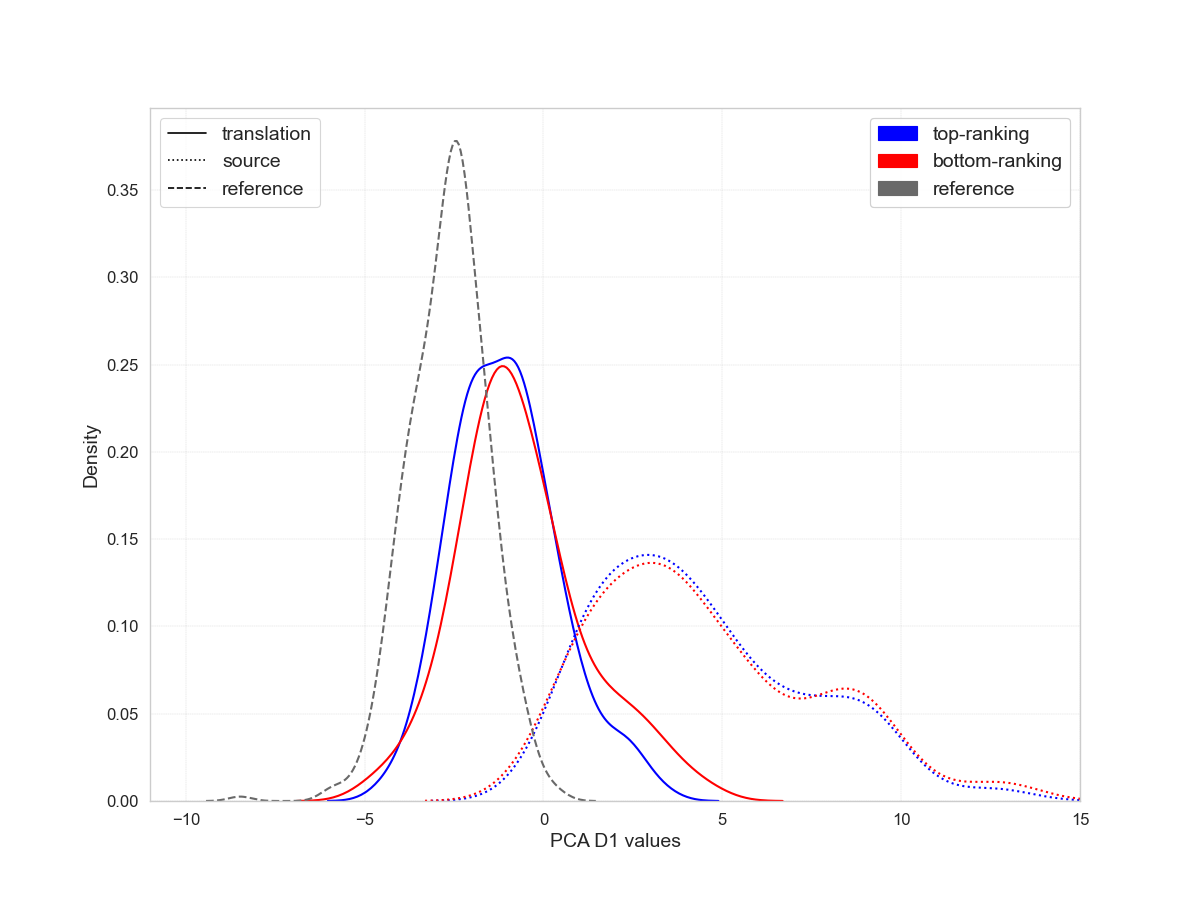
\includegraphics[width=\linewidth]{figures/pca/src-qua-ttype-ud-PCA-D1-lines}
	\end{minipage}	
	\begin{minipage}[c]{0.5\linewidth}
		\centering
		\textit{mdeberta3} PCA D1
		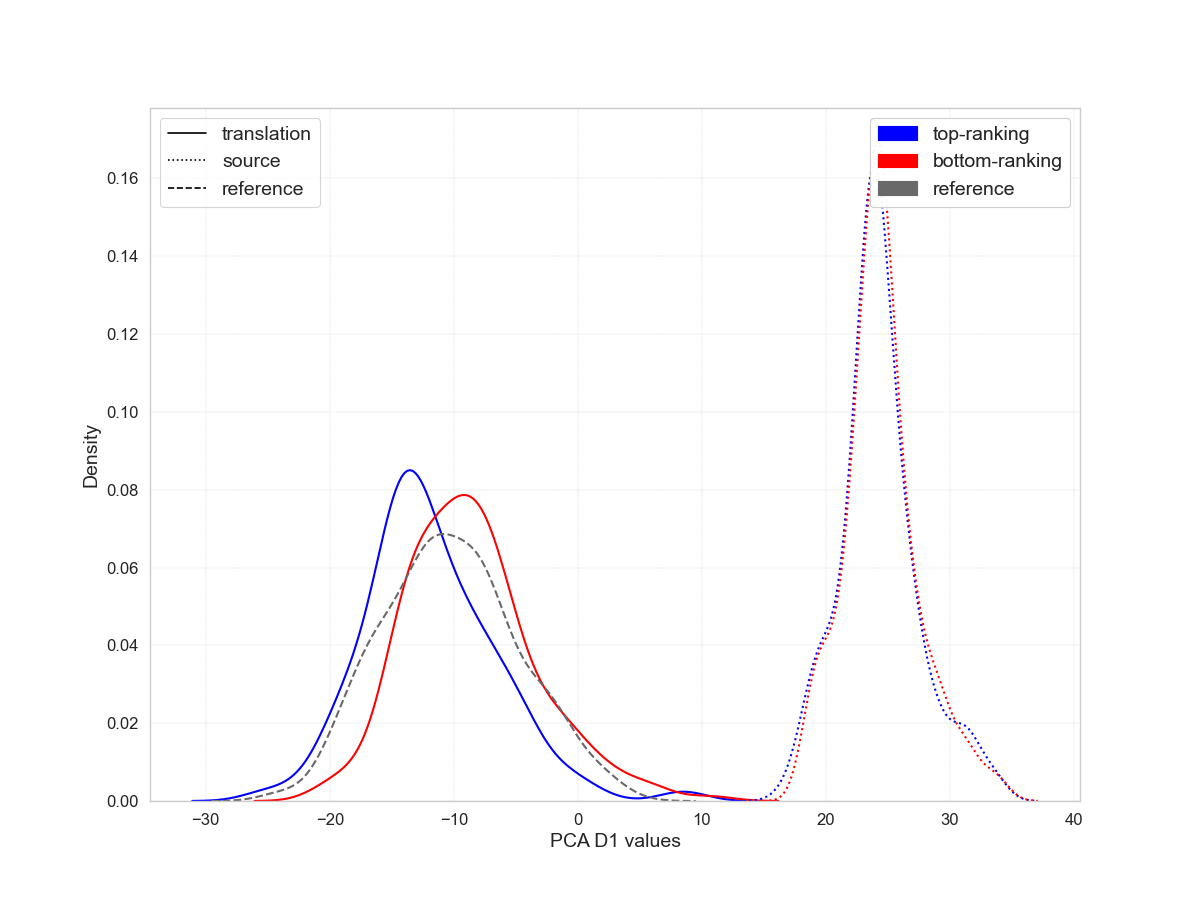
\includegraphics[width=\linewidth]{figures/pca/src-qua-ttype-mdeberta3-base-PCA-D1-lines}
	\end{minipage}
	\caption{\label{fig:pca_qua}Variability of PCA D1 values in quality-annotated documents (along with their sources and non-translations)}	
\end{figure}   

In turn, this suggests that the quality distinctions captured by \textit{mdeberta3} are, in fact, related to translationese, interpreted as the amount of deviations from the TL norm, especially on the axis capturing language contrast.
\begin{figure}[H]
	\begin{minipage}[c]{0.5\linewidth}
		\centering
		Top 26 UD features PCA D1
		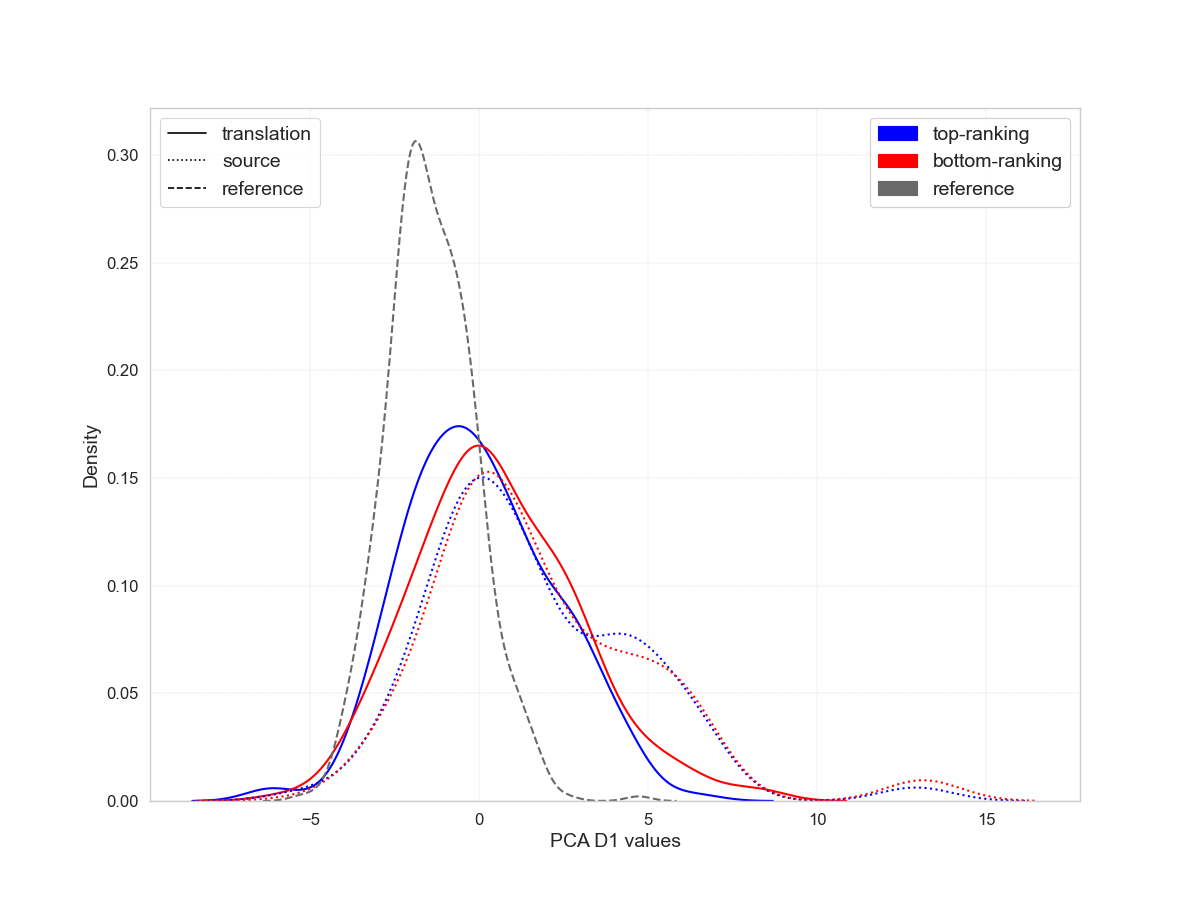
\includegraphics[width=\linewidth]{figures/pca/src-bad-good-pca-ud26-D1-lines}
	\end{minipage}	
	\begin{minipage}[c]{0.5\linewidth}
		\centering
		\textit{mdeberta3} PCA
		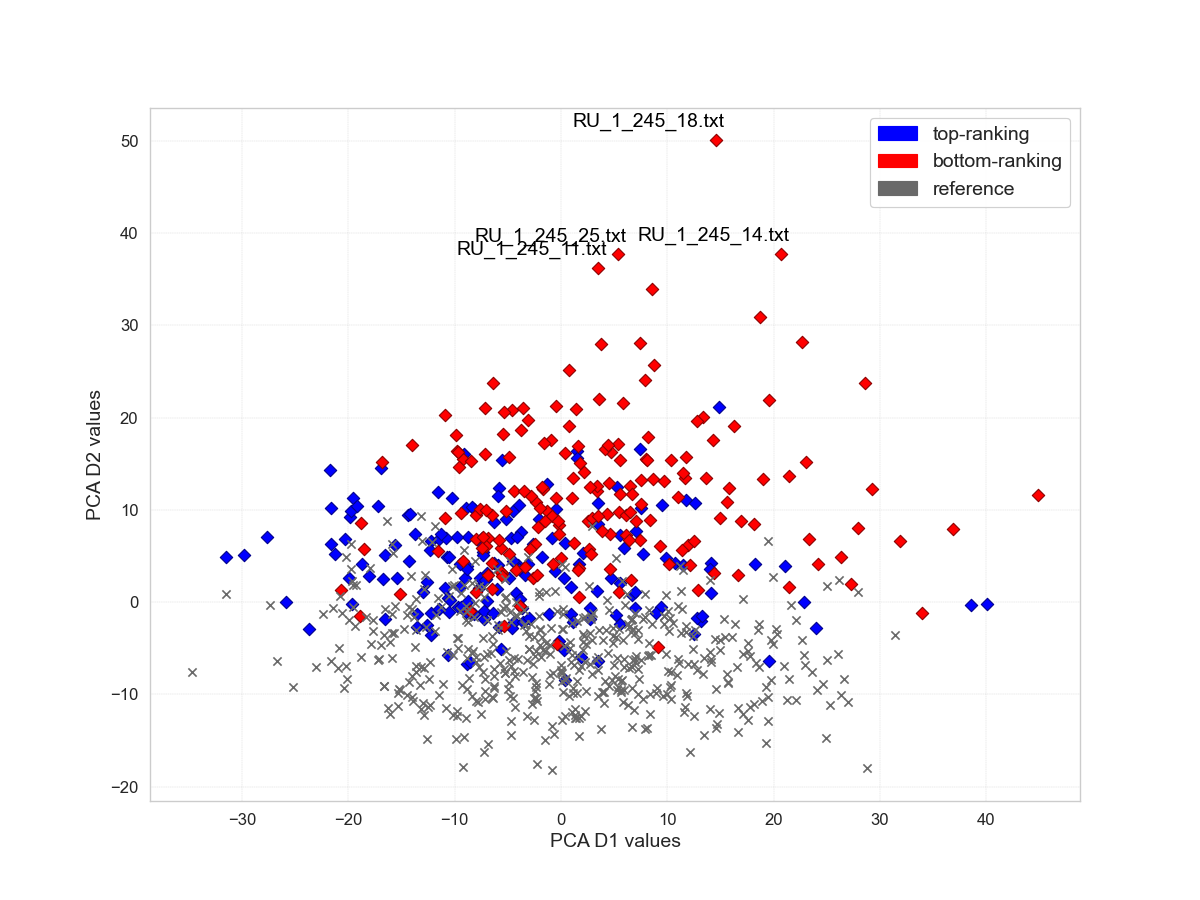
\includegraphics[width=\linewidth]{figures/pca/qua-ttype-mdeberta3-base-PCA-scatter}
	\end{minipage}
	\caption{\label{fig:pca_qua26}Variability of PCA D1 values in quality-annotated documents (no source texts)}	
\end{figure}
However, as we have seen in the feature analysis for student translations in Section~\ref{ssec:best_ud}, shining-through does not exhaust translationese manifestations. Plotting the PCA results for just the best performing subset of UD features eliminated the distinctions between languages (compare the left-hand panels in Figures~\ref{fig:pca_qua} and~\ref{fig:pca_qua26}). This might mean that some of the 26 selected features (see below) are not necessarily shining-through indicators. Translation quality is partly captured along other dimensions of translated language, not just the one defined by the contrast between languages. 

The right-hand panel in Figure~\ref{fig:pca_qua26} demonstrates that the PCA transform of the \textit{mdeberta3} captures the quality parameter of the dataset on the orthogonal PCA dimension (D2): the lower-ranking translations (in red) can be identified as more distant from TL norm (grey cloud). 
% RU_1_245_25.txt
%RU_1_245_11.txt
%RU_1_245_18.txt
%RU_1_245_14.txt

\paragraph{\label{pg:selection_helps_in_quality_classification}Feature analysis} 
Almost half of 26 most contributing UD features selected by RFECV in the classification task on quality labels were in the intersection with strong translationese indicators identified in Section~\ref{ssec:best_ud}. This selection significantly improved the performance of the SVM classifier: F1-score went up by 8\% from 61.0 to 68.9\%. 
%68.86 (+/-7.15)
%T-TEST: svm_bad-good_ud26 is significantly better with F1-score = 0.6886167230000001

Table~\ref{tab:bad-good_indicators} aggregates parameters that characterise each feature in this selection from the point of view of: (1) ability to predict quality categories alone (for features with statistically significant differences between the categories, otherwise `--' in \textit{LogR} column), (2) comparison of mean feature values across the categories, (3) SVM weights assigned to each feature and (4) translational trend in `bad' translations. 
The hypothesised trend is shown in bold if there were significant differences between `good' and `bad' categories. The regular font is used if there were significant differences between some of the three document categories involved in the comparison (src, bad, ref). In cases where there were no distinctions between the three categories, it was difficult to talk about any trend (--). The table is sorted by SVM weight.
% for intersection with pro, it is everything except case
% for intersection with student: not used for qua 7 of 14: 'aux', 'superl', 'xcomp', 'infs', 'mhd', 'nn', 'content_dens'

%Best Feats within levels with skewed distributions (4): ['good_adp', 'bad_adp', 'bad_mdd', 'bad_simple']
%Best Feats with unequal variances (22): ['adp', 'attrib', 'caus', 'content_TTR', 'deverbals', 'mdd', 'mpred', 'mquantif', 'numcls', 'possp', 'pverbals', 'sentlength', 'simple', 'advcl', 'amod', 'appos', 'aux:pass', 'conj', 'iobj', 'nummod', 'obj', 'parataxis']

%Strong translationese indicators useful for quality classification (12):{'advcl', 'attrib', 'acl:relcl', 'nsubj', 'pverbals', 'aux:pass', 'mark', 'obj', 'sentlength', 'amod', 'simple', 'deverbals'}

% it would be useful to add ref and type of trend to this table!!!
\begin{longtable}{l|llcc}
%	\centering
%	\begin{tabular}
		\midrule
		feature      & LogR         & means            & SVM weight &  trend in `bad' \\
		\midrule
		\textbf{sentlength}   & --           & bad=>good & 1.616 & NA  \\
		\textbf{nsubj}        & 0.13 +/-0.12 & bad>src>good>ref & 1.06  & \textbf{anglicisation} \\
		\textbf{amod}         & --           & bad=>good=>ref>src & 0.857 & adaptation \\
		\textcolor{Dandelion}{numcls}       & -- & bad>good>src=>ref & 0.713 & SL/TL indep \\
		\textbf{attrib}       & --           & bad=>good=>ref>src & 0.623 & adaptation \\
		\textbf{acl:relcl}    & 0.13 +/-0.09 & src>bad>good>ref & 0.615 & \textbf{shining} \\
		\textbf{simple}       & --           & src>ref=>bad=>good* & 0.563 & adaptation \\
		\textbf{advcl}        & 0.13 +/-0.07 & src>bad>good>ref & 0.521 & \textbf{shining} \\
		\textbf{aux:pass}     & --           & src>bad=>ref=>good & 0.491 & adaptation \\
		\textbf{deverbals}    & --           & bad=>good=>ref>src & 0.477 & adaptation \\
		\textbf{obj}          & --           & src>bad=>good>ref & 0.44  & shining \\
		\textcolor{cadmiumgreen}{content\_TTR} & 0.00 +/-0.00 & bad<good<=src<=ref & 0.416 & \textbf{SL/TL indep} \\
		\textbf{mark}         & --           & src>bad=>good>ref & 0.409 & shining \\
		\textcolor{Dandelion}{parataxis}    & --  & src<bad<=good<ref    & 0.397 & underuse of TL \\
		conj         & --           & bad=>good>src=>ref & 0.389 &  SL/TL indep \\
		\textcolor{cadmiumgreen}{passives}     & 0.05 +/-0.08 & src<bad<good<ref & 0.32 & \textbf{underuse of TL} \\
		\textcolor{Dandelion}{iobj}    & 0.05 +/-0.13 & src<bad<good<ref & 0.319 & \textbf{underuse of TL} \\
		\textcolor{Dandelion}{nummod}  & -- & ref=>bad=>good>=src* & 0.318 & -- \\
		\textcolor{cadmiumgreen}{mdd}  & -- & ref<bad<=good<src*    & 0.316 & normalisation \\
		\textbf{pverbals}     & --     & ref>bad=>good>src* & 0.289 & normalisation  \\
		\textcolor{cadmiumgreen}{adp}  & -- & src=>ref=>bad=>good & 0.254 & -- \\
		\textcolor{Dandelion}{mquantif}& -- & bad<=good<=ref<src & 0.244 & underuse of TL  \\
		appos        & --           & bad=>good=>ref=>src & 0.23 & --  \\
		possp        & --           & src<ref<=bad<=good*    & 0.202 & adaptation \\
		\textcolor{Dandelion}{caus} & -- & ref<=src<=bad<=good*  & 0.195 & -- \\
		\textcolor{Dandelion}{mpred} & -- & src>bad=>good>ref & 0.116 & shining \\
		\midrule
		\textbf{copula}       & 0.14 +/-0.12 & src>bad>good>ref &  & \textbf{shining}           \\
		\textbf{finites}      & 0.09 +/-0.13 & src>bad>good>ref &     & \textbf{shining}      \\
		\textcolor{Dandelion}{infs}         & 0.08 +/-0.09 & src<bad<good<ref    &  & \textbf{shining}          \\		
		\bottomrule
%	\end{tabular}
\caption{\label{tab:bad-good_indicators}Features selected by RFECV with results of significance testing and comparison between document categories. The fonts and colours in the \textit{feature} column indicate whether the feature is among the strong translationese indicators shared by both professional varieties (bold), or comes from the features selected as predictors of only professional (green) or student translation (orange)}\\
\end{longtable}
Features that were also identified as strong translationese indicators in previous analysis (see Section~\ref{ssec:best_ud}) are shown in bold in \textit{feature} column. Translationese features that were specific for either professional or student translations are shown in green and orange, respectively, as they were colour-coded in Section~\ref{sec:detect}. There were only three quality indicators that were not associated with translationese: \textit{frequency of syntactic conjuncts (\textit{conj}), appositive constructions (\textit{appos}) and possessive pronouns (\textit{possp})}.
In \textit{means} column we used \textit{<=} and \textit{=>} signs to signal the comparison between categories, even in the absence of statistically significant differences.
The last three features in Table~\ref{tab:bad-good_indicators} had significant differences between the document categories in univariate analysis, but they were not selected as useful in quality classification (\textit{copula verbs, verbs in finite form and infinitives}). 
%Copula verbs and finite verb forms were among shared translationese indicators, while frequency of infinitives was useful to separate student translations from non-translations.

As can be seen from Table~\ref{tab:bad-good_indicators}, SVM classifier operated in the feature space where only a few features had statistically significant distinctions. All features had modest association with the labels, too. It is not surprising as this experiment was run on a relatively small dataset.
Nonetheless, it can be seen that in cases of significant difference between quality categories, \textit{bad} translations mostly passively followed SL patterns. This behaviour consists in either carrying over the items with higher SL frequencies (anglicisation, shining-through) or in lack of ability to come up with preferred TL patterns, where the frequencies in TL are higher than in the SL (\textit{underuse of TL}). 
Most comparisons (even if insignificant) showed that \textit{good} translations were almost always closer to the TL reference than \textit{bad} translations (the six exceptions from this observations are marked with an asterisk in Table~\ref{tab:bad-good_indicators}).  

Figure~\ref{fig:qua-weights} visualises the contribution of each feature to the improved classifier. 

We omitted the analysis of QuEst++ features on this dataset due to its poor performance, which was even lower than the random baseline.

Concluding the observations from the experiments on document labels, let us see whether there were commonalities between the outcomes of professionalism and quality classifications. 

\begin{figure}[H]
	\centering
	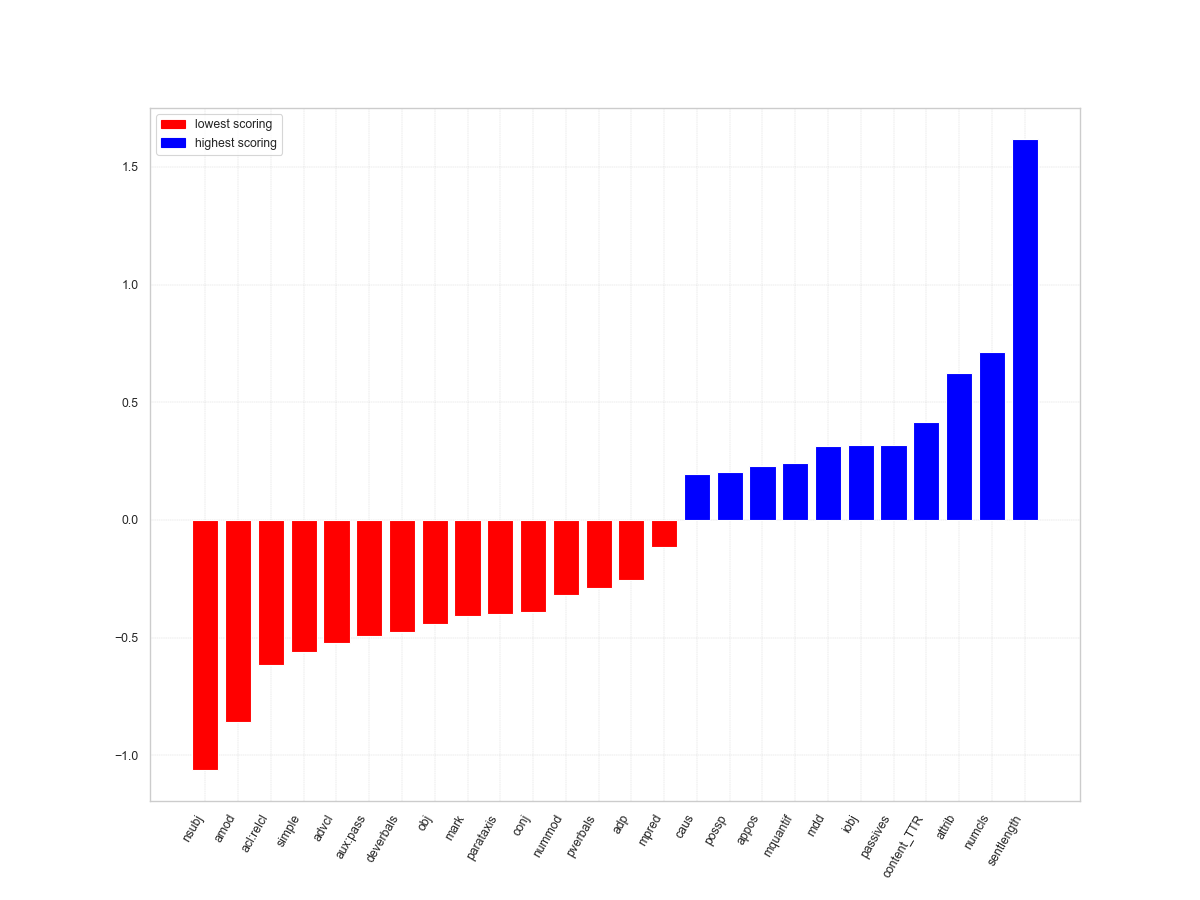
\includegraphics[width=.80\linewidth]{figures/bad-good-bars-ud26}
	\caption{\label{fig:qua-weights}Weights loading the decision towards each category for 26 RFECV-selected items}	
\end{figure}

Although the classification results on UD features were higher in professional variety classification than in translation quality classification (79.39\% vs 68.9\% on the best-performing subsets of features), we would argue that translationese is more related to quality than to professionalism. Analysis in Sections~\ref{ssec:var} (page~\pageref{pg:more_professional_more_translated}) demonstrated that some translationese features were actually more typical to professional translations than to student translations. This finding was against our expectations, but helped the classifier. 
However, quite in line with the expected, the properties of \textit{bad} translations on most translationese features indicated that these translations had major deviations from the expected TL norm. %, mostly because they carried over ST features. 
%There were only two strong translationese predictors that worked for predicting both varieties and quality: (\hyperlink{acl:relcl}{relative clauses}, \hyperlink{mark}{subordinate clause introducers}).
%Interestingly, there were two features that were useless for any translationese classification among the other six features shared by professionalism and quality classifiers (\hyperlink{appos}{paranthetical modifiers of nouns}, \hyperlink{conj}{syntactic conjuncts}).  % we are talking here about the intersection of \hyperlink{wd:15best-var}{15} and 26 features.
\label{pg:bad_tendencies}
It means that distinctions between professional varieties and quality categories run along different directions. \textbf{Professional translations do not necessarily exhibit less translationese than student translations, while lower-ranking translations do demonstrate stronger translationese tendencies.} In particular, \textit{bad} translations feature longer sentences, more complex sentence structure (more clauses, especially relative clauses), lower TTR, more analytical passives and fewer passive constructions, more nouns functioning as subjects, more modal predicates, more verbal forms, including overuse of copula verbs, deverbal nouns and participles. 

% Following the suggestion by~\ref{Aharoni2015} who relied on boolean vectors reflecting usage of PoS, listed function words and context free grammar rules to predict MT quality, we implemented an additional SVM quality classifier using probabilities for translated class from student translationese classification on best-performing features as a single input. This classifier achieved F1-score of ???? for `bad' vs `good' experiment.

%Inspired by \cite{Aharoni2014} results for French-English MT, showing that the higher the translationese classification accuracy, the lower the expected translation quality, this research applies a similar approach in the domain of human English-to-Russian translation.

\section{\label{sec:_scores}Regression Tasks}
The purpose of this section is to compare the performance of SVM on document-level datasets with two types of quality scores: a score derived from error annotation and a score obtained through direct assessment.

We want to find out which approach to benchmarking quality by human judges is better aligned with the objective properties of translations as captured by our representations, with a focus on the established translationese indicators.

\subsection{\label{ssec:my_doc_regressors}Experimental Setup}

\paragraph{Datasets} 
The input for the quality prediction tasks, formulated as regression problems, was stored in a separate table of the structure similar to the dataset with document-level labels. It included instances in rows and features in columns. All tested scores, sentence-aligned documents and their lemmatised versions were added as columns as well. 
%It included the total of 1106 instances (rows). 
The intersection between quality-labelled and quality-scored student translations included about 17\% of the total number of unique student translations used in this thesis (206 of 1222 documents). 
Therefore, the datasets were kept separate.

In brief, the error-annotated subcorpus consists of 553 parallel documents, 140 of which are also annotated with DA scores. Both collections include multiple translations for 46 and 30 STs, respectively.
The quality scores were generated as described on page~\pageref{pg:tq} in Section~\ref{ssec:err} for error-based scores and on page~\pageref{pg:final_da} in Section~\ref{ssec:da} for scores from direct assessment. 
In particular, the quality scores included:
\begin{description}\compresslist{}
	\item[accuracy:] frequency of content errors weighted for error categories and normalised to the ST word count,
	\item[fluency:] frequency of language errors weighted for error categories and normalised to the ST word count,
	\item[tq:] overall quality score and its variant (\textbf{scaled\_tq}) transformed into the 0-100 range,
	% as follows scaled_score = (((100 - 0) * (score_current - minscore)) / (maxscore - minscore)) + 0
	\item[da\_mean:] document-level scores from DA averaged from sentence-level and their z-transformed variant (\textbf{da\_zmean}).
\end{description}

\paragraph{Representations}

We used the same representations as for the labelled datasets. 
Given the poor performance on \textit{collgram}- and \textit{ngram}-based features and on \textit{stsb-xlm-r-m} vectors in the classification tasks, we omit them from the results in regression experiments reported in this section. 
% this is a bad decision if we contend that error-based scores have a different perspective on quality.

\paragraph{Learning algorithm and evaluation setup}
% regressor = SVR(kernel='rbf', degree=3, gamma='scale', coef0=0.0, tol=0.001, C=1.0, epsilon=0.1, max_iter=-1, shrinking=True)
For translated documents with quality scores, the ML task is formulated as a regression problem. We learn the target scores using \gls{SVR} as implemented in \textit{scikit-learn}, with the library default settings. In particular, the algorithm uses \textit{radial basis function (rbf)} kernel, with \textit{gamma} parameter set to `scale', \textit{C} to 1.0 and \textit{epsilon} to 0.1.
We omit the results for the neural regressor, because they are not different from SVR performance in a principled way as was the case in Sections~\ref{sec:detect}, \ref{ssec:var} and~\ref{ssec:bin}.

The performance of \gls{SVR} is reported in terms of Spearman's rank correlation coefficient (r) and \gls{RMSE}. The former is selected because the quality scores are not normally distributed especially at sentence level (see Figures~\ref{fig:sents_weighed_aspects} and~\ref{fig:sents_tq} on page~\pageref{pg:skews} in Chapter~\ref{cha:quest}). \gls{RMSE} helps to keep track of the magnitude of errors in predicted scores. This metric is typically used in the quality estimation shared tasks by \gls{WMT}.

\paragraph{Feature analysis methods}
The strength of the relationship between each variable (feature) and target labels was measured using 5-fold cross-validated \textit{linear regression} which returned Spearman's correlation coefficient for continuous response variable (scores) in a regression task. 

% MAE measures the average magnitude of the errors in a set of predictions, without considering their direction. It’s the average over the test sample of the absolute differences between prediction and actual observation where all individual differences have equal weight.

%RMSE is a quadratic scoring rule that also measures the average magnitude of the error. It’s the square root of the average of squared differences between prediction and actual observation.

% Since the errors are squared before they are averaged, the RMSE gives a relatively high weight to large errors. This means the RMSE should be more useful when large errors are particularly undesirable. 

% Both MAE and RMSE express average model prediction error in units of the (dependent) variable of interest. Both metrics can range from 0 to ∞ and are indifferent to the direction of errors. 

% They are negatively-oriented scores, which means lower values are better.

% RMSE has a tendency to be increasingly larger than MAE as the test sample size increases
% This can problematic when comparing RMSE results calculated on different sized test samples, which is frequently the case in real world modeling.

% RMSE increases as the variance associated with the frequency distribution of error magnitudes also increases. RMSE does not necessarily increase with the variance of the errors. RMSE increases with the variance of the frequency distribution of error magnitudes.
\subsection{\label{ssec:doc_err_res}Document Level: Error-based Scores}
Based on the existing error annotation, we generated three quality scores. Accuracy and fluency score were calculated from content and language error frequencies, respectively. Overall translation score (tq) was obtained using raw overall error statistics. All scores were normalised to the ST word count.
In an attempt to generate more theoretically justified scores, we also produced a weighted version of these scores using an elaborate weighting scheme. \textit{Weighted} accuracy and fluency scores in Table~\ref{tab:docs_err_par} take into account severities of errors (e.g. a critical error weights more than a minor error). Additionally, these scores are weighted by individual categories of content and language errors as recommended by \textit{TAUS}. For example, an error in collocation has a greater weight than a spelling error. 
The overall quality score uses the severities and annotated positive assessment (kudos) in its weighted variant. This explains why tq score can go over the maximum bound of the absolute scale (100). Scaled tq score is tq score re-calculated for a 0-100 scale, using Formula~\ref{eq:squeezeit}:
\begin{equation}\label{eq:squeezeit}
\begin{split}
scaled score = \frac{100\times (score - min)}{max - min} \\
\end{split}
\end{equation}
where \textit{score} is normalised error frequency, \textit{min} and \textit{max} are respective values of the unscaled score range.

The scaling was done to put the scores from error annotation on the same measuring scale as DA scores. Detailed account of converting error statistics to scores is given in Section~\ref{ssec:err} (see page~\pageref{pg:err-score-generation}). 

Table~\ref{tab:docs_err_par} has the parameters of each quality score distribution (across 553 translations). Note that weighted scores are better distributed across the 0-100 scale, while unweighted scores are hurdled around the maximum value.
\begin{table}[H]
	\centering
	\begin{tabular}{l|ccc}
		\toprule
		& Min   & Max    & Mean (+/-STD)  \\
		\midrule
		\multicolumn{4}{c}{Unweighted scores} \\
		\midrule
		accuracy   & 93.55 & 100    & 98.12 (+/-1.04)  \\
		fluency    & 90.88 & 99.8   & 97.36 (+/-1.32)  \\
		tq         & 87.62 & 99.56  & 95.49 (+/-1.92)  \\
		scaled\_tq & 0     & 100    & 65.86 (+/-16.04) \\
		\midrule
		\multicolumn{4}{c}{Weighted scores} \\
		\midrule
		accuracy   & 61.28 & 98.9   & 86.03 (+/-6.69)  \\
		fluency    & 59.21 & 98.46  & 86.52 (+/-6.11)  \\
		tq         & 72.67 & 100.36 & 92.69 (+/-4.35)  \\
		scaled\_tq & 0     & 100    & 72.3  (+/-15.72) \\
		\bottomrule
	\end{tabular}
	\caption{\label{tab:docs_err_par}Quantitative parameters of error-based scores across 553 documents}
\end{table}

Table~\ref{tab:doc_err_double} has the results of the document-level regression tasks for the error-based scores across seven representation.
\paragraph{\label{pg:doc_err_ud_vs_all}Performance of UD against other representation}
Similar to classification experiments on quality labels, morphosyntactic features, proposed in this thesis, were significantly outperformed only by \textit{mdeberta3} on unweighted accuracy and tq scores, and by \textit{mdeberta3} and \textit{ruRoberta} on fluency.
\vspace{-1.5em}

\begin{table}[H]
	\centering
	\begin{tabular}{l|cl|cl|cl|cl}
		\toprule
		& \multicolumn{2}{c|}{accuracy} & \multicolumn{2}{c|}{fluency}  & \multicolumn{2}{c|}{tq} & \multicolumn{2}{c|}{scaled\_tq}    \\
		\midrule
		\multicolumn{9}{c}{Unweighted scores} \\
		\midrule
		       & \textit{r}  & RMSE & \textit{r}  & RMSE & \textit{r}  & RMSE & \textit{r} & RMSE  \\
		\midrule
			UD     & \textbf{0.43} & 0.95 & \textbf{0.43} & 1.18 & \textbf{0.45} & 1.72 & 0.32 & 15.5  \\
			all             & 0.41 & 0.96 & 0.43 & 1.19 & 0.43 & 1.74 & 0.32 & 15.56 \\
			quest61         & 0.37 & 0.98 & 0.42 & 1.16 & 0.36 & 1.73 & 0.31 & 15.22 \\
			\midrule
			tfidf           & 0.48 & 0.92 & 0.49 & 1.14 & 0.47 & 1.69 & 0.39 & 15.59 \\
%			\midrule
			TQmono-m        & 0.46 & 0.94 & 0.47 & 1.15 & 0.45 & 1.68 & 0.35 & 15.3  \\
			ruRoberta & 0.51 & 0.91 & 0.53 & 1.08 & 0.54 & 1.57 & 0.44 & 14.84 \\
			mdeberta3  & 0.58 & 0.87 & 0.58 & 1.05 & 0.62 & 1.5  & 0.56 & 14.62 \\
		\midrule
		\midrule
		\multicolumn{9}{c}{Weighted scores} \\
		\midrule
		UD              & 0.38 & 6.31 & 0.37 & 5.72 & 0.44 & 4.02 & \textbf{0.38} & 15.13 \\
		all             & 0.38 & 6.34 & 0.35 & 5.77 & 0.43 & 4.06 & 0.36 & 15.18 \\
		quest61         & 0.32 & 6.34 & 0.33 & 5.68 & 0.37 & 4.1  & 0.33 & 15.13 \\
		\midrule
		tfidf           & 0.4  & 6.36 & 0.39 & 5.78 & 0.48 & 4.04 & 0.45 & 15.23 \\
%		\midrule
		TQmono-m        & 0.4  & 6.13 & 0.37 & 5.64 & 0.47 & 3.92 & 0.38 & 14.85 \\
		ruRoberta & 0.48 & 5.98 & 0.45 & 5.47 & 0.57 & 3.74 & 0.5  & 14.53 \\
		mdeberta3  & \boxit{0.3in}0.62 & 5.76 & \boxit{0.3in}0.59 & 5.21 & \boxit{0.3in}0.67 & 3.54 & \boxit{0.3in}0.63 & 14.19 \\
		\bottomrule
	\end{tabular}
\caption{\label{tab:doc_err_double}Regression results for error-based quality scores (553 documents). For each quality score, the boldface type is used to denote the highest $r$ for manual features; the highest $r$ for content-dependent representations is boxed}
\end{table}

The highest result of $r=0.67$ was seen on \textit{mdeberta3} representations for weighted overall quality (cf. $r=0.45$ for UD features). % not significantly outperformed in any other setting
As expected, \textit{collgram} and \textit{ngram} features implicitly present in \textit{all} were not helpful and introduced noise, showing slightly lower performance than UD feature set across all scores. 
Interestingly, a custom \textit{tf-idf} representation\wlvfootnote{produced on lemmatised corpus with proper names and numbers substituted with respective placeholders, see page~\pageref{pg:tfidf_meth}} consistently performed better than both morphosyntactic features and TQ-estimation-dedicated cross-lingual sentence embedding model from \textit{TransQuest} in absolute terms, but we do not have enough data to see statistically significant results on these comparisons.

Table~\ref{tab:doc_err_double} omits STD values for brevity. These values for $r$ vary in the following ranges across representations: accuracy (0.07--0.10), fluency (0.09--0.12), tq (0.08--0.13), scaled\_tq (0.06--0.12).

\paragraph{Comparison of regressors across types of scores}
From Table~\ref{tab:doc_err_double}, Spearman's \textit{r} was higher for overall quality score (tq) than for accuracy, fluency or scaled\_tq for both weighted and unweighted versions. However, most differences between the results on accuracy, fluency or tq were not statistically significant. Whenever there was a significant difference (mostly between weighted fluency and tq), the results were always better for tq.

Significant differences between weighted and unweighted versions were seen only for fluency on \textit{ruRoberta} and for scaled\_tq on \textit{mdeberta3}. However, it is impossible to say which version of scores was more learnable because the unweighted score returned higher results in the former setting and the weighted score was superior in the latter. 
It is noteworthy that weighted scores returned much larger error between the gold scores and predictions as measured by \gls*{RMSE}. 
Based on these observations, {unweighted scores are preferable to weighted scores}.

\textbf{Scaled version of the overall quality scores was inferior to unscaled version} on almost all representations. % for all representations except \textit{mdeberta3} on unweighted scores. 
Scaling the quality score tripled the average prediction error, too.
In the subsequent experiments reported in this chapter, weighted scores and scaled version of overall quality (scaled\_tq) are excluded from the analysis.

These results draw attention to a curious finding. Contrary to the expectations, we did not see statistically significant differences between accuracy and fluency in terms of performance on any representations, including translationese features. If these scores captured independent aspects of quality, we would expect higher results for fluency on our TL-centred representations. We can cautiously suggest that \textbf{our data did not contain translations that were very inaccurate but fluent, and vice versa}. The two aspects of quality seem to be correlated. Indeed, on weighted scores, Spearman's correlation coefficient between them was 0.897\wlvfootnote{Intuitively, the weighted scores, which take into account the type of errors and their severities, reflect the actual opinion of assessors' on quality}. % $r=0.309$ on unweighted scores based on simple normalised frequency of content and language errors disregarding severities or subtypes of these major categories
This might mean that \textbf{an \gls*{HTQE} approach aimed at fluency can be a useful proxy for overall document-level quality from error annotation}.
Another explanation is lack of training data. Our experiments were run on 553 annotated translations and did not reveal the differences between the two aspects of quality. If more data is needed to reveal these differences, then the differences must be really small. 
%A more plausible explanation is that \textbf{scores from error annotation do not reflect translationese properties of translations, at least when they are generated for entire documents}. %; language errors are focused on other imperfections of student translations. 

\paragraph{Feature analysis} 
Feature selection for UD set did not yield any sizeable improvements in performance on either weighted or unweighted scores. 
On weighted scores, the maximum gain was for accuracy, where the value for correlation coefficient went up from 0.38 to 0.42 on a selection of 29 features. On unweighted scores, a selection of 44 UD features increased the regression result on accuracy only by 0.01 (from 0.43 to 0.44). 

Limiting QuEst++ feature set to the best-performing 21 features resulted in a very modest gain of 0.03 on accuracy. % on random 140 docs 9 QuEst++ achieve the same result: ['bqe_1009', 'qe_1026', 'qe_1032', 'bqe_1053', 'bqe_1054', 'bqe_1074', 'qe_9994', 'qe_9995', 'qe_9996']
No selection of features was able to improve the performance on fluency and tq scores for either UD or QuEst++. 

To reveal the features that were better correlated with various quality scores, we used each of them as a single input to a \textit{linear regression} algorithm as implemented in \textit{scikit-learn}, with the library default parameters.  % Logistic regression is switched to linear regression because we use continuous instead of categorical quality estimate

Univariate correlation analysis did not reveal any features from UD, collgram, ngram or QuEst++ feature sets that were associated with any quality score for more than Spearman's $r=0.274$. % Interestingly, the values of $r$ between any single feature and (best-performing) fluency scores were more than 1.5 times lower than for accuracy or tq. % I am not sure how to explain this.
% the highest r (positive or negative seen for collgram, ngram was on unweighted tq: bigram-tscore_std   0.189) 
\label{pg:scores_not_translationese}
Although the correlation between the proposed quality indicators and various quality scores was small, we noticed that some important quality predictors from UD features (from the top 10 better-correlated features) contributed to all scores while others remain specific to accuracy or fluency. The intersection of top 10 features by correlation with unweighted accuracy, fluency and tq included \textit{nsubj, acl:relcl, obj}. These relatively strong predictors shared by all error-annotated scores capture syntactic complexity of sentences in translations: number of explicit syntactic subject and object dependencies across all clauses (\textit{nsubj}, \textit{obj} and number of relative clauses (\textit{acl:relcl})). All of them were weakly but positively correlated with the scores. This brings us to a counter-intuitive conclusion that the more well-developed finite clauses there were in the sentence, the higher was the quality score. This also contradicts the results on binary labels (see page~\ref{pg:bad_tendencies}).

One way to interpret this contradiction is to suggest that holistic document-level perception of quality incorporated translationese-related properties of translations, while error-based quality scores, even from fluency errors, did not reflect translation solutions that can be explained by translationese. 
The fact that prominent quality predictors were equally associated with accuracy, fluency and tq, together with the observation that this association was weak ($r<0.243$), confirms that even if accuracy and fluency reflected different aspects of translation quality, these aspects were not related to translationese.

\label{pg:errors_some_coherence_with_translationese_theory_of_quality}
A look at other translationese features that were found among the top 10 by correlation with either accuracy or fluency suggests an interpretation coherent with the translationese hypothesis of quality for some of them. 
For example, accuracy scores returned $r=0.226$ for Spearman's correlation with the frequency of negative particles. This aligns well with the translationese explanation: the more negative particles, the higher the translation quality. Less fluent translations tend to underuse negative constructions and follow the English affirmative way of expression. Accuracy scores also had $r=-0.1$ correlation with epistemic markers. The overuse of literal translations for the phrases like \textit{certainly, as far as we know, of course, no doubt, it appears that}, which are more common in English, seemed to predict lower-ranking translations. The most prominent indicator of fluency was the frequency of modal predicates ($r=-0.106$). From translationese theory perspective, the overuse of modal predicates in English-to-Russian translation signals lower quality.
Even if these observations are acceptable, they do not explain either error-based scores or the difference between them convincingly due to their low potency.   

\label{pg:quest_feats4err}
The comparable \textbf{performance of QuEst++ for all error-based scores was based on ST complexity features}.
For the QuEst++ feature set, the intersection between best-performing features on accuracy and fluency included six out of 10 top features. Five of them were complexity (ST-based) features that \textit{measured average number of translations per source word} counted with various Giza probability thresholds (including \#1016, \#1018, \#1020, \#1022, \#1024, e.g. document-level QuEst++ feature \#1024: ``average number of translations per source word in the sentence (threshold in giza1: prob > 0.05)''). Apart from that, number of sentences in the target document (\#9801) was relatively well correlated with all scores. It indicated that the more sentences there were in a translation, the higher was the quality score.
The error-annotated dataset included multiple translations for 47 English sources. Apparently, the differences between them were most contributive to the QuEst++ regressor performance. We looked through the extended lists of top 15 most-associated features for accuracy and fluency, and found that they represented the properties of ST (with the exception of two adequacy features). Over-reliance of this classifier on the ST side fits well with no distinction between accuracy and fluency. Indeed, a more demanding ST can trigger both content and language errors, as we demonstrated in~\cite{Kunilovskaya2023err}.
However, it also shows that QuEst++ feature set did not pick up any relevant distinctions between translations per se. 
%Analysis of intersections in \textit{tf-idf} top features did not reveal any patterns and was not enlightening. 

%fluency	
%qe_1024	average number of translations per source word in the document (threshold in giza1: prob > 0.5)
%qe_9801	Number of sentences in the source document
%qe_1016	average number of translations per source word in the sentence (threshold in giza1: prob > 0.01)
%bqe_1001	number of tokens in the source document
%qe_1018	average number of translations per source word in the sentence (threshold in giza1: prob > 0.05)
%qe_1020	average number of translations per source word in the sentence (threshold in giza1: prob > 0.10)
%bqe_1022	average number of translations per source word in the sentence (as given by IBM 1 table thresholded so that prob(t|s) > 0.2)
%bqe_1046	average unigram frequency in quartile_1 of frequency (lower frequency words) in the corpus of the source document
%qe_1059	percentage of distinct bigrams seen in the source corpus (in all quartiles) - document-level
%qe_1004	no tokens in the target / no tokens in the source
%qe_1026	average number of translations per source word in the document (threshold in giza1: prob > 0.01) weighted by the frequency of each word in the source corpus")
%qe_1032	average number of translations per source word in the document (threshold in giza1: prob > 0.2) weighted by the frequency of each word in the source corpus")
%qe_1093	ratio of percentage of verbs in the source and target documents
%
%accuracy	very 
%qe_1056	average trigram frequency in quartile 3 of frequency (lower frequency words) in the corpus of the source document
%qe_1085	ratio of percentage of content words in the source and target documents
%qe_1089	percentage of verbs in the source document
%qe_1052	average bigram frequency in quartile 3 of frequency (lower frequency words) in the corpus of the source document
%bqe_1050	average bigram frequency in quartile 1 of frequency (lower frequency words) in the corpus of the source document
%qe_1093	ratio of percentage of verbs in the source and target documents
%qe_1024	average number of translations per source word in the document (threshold in giza1: prob > 0.5)
%qe_9801	Number of sentences in the source document
%qe_1016	average number of translations per source word in the sentence (threshold in giza1: prob > 0.01)
%qe_1018	average number of translations per source word in the sentence (threshold in giza1: prob > 0.05)
%qe_1020	average number of translations per source word in the sentence (threshold in giza1: prob > 0.10)
%bqe_1022	average number of translations per source word in the sentence (as given by IBM 1 table thresholded so that prob(t|s) > 0.2)

% for weighted scores
% Selected accuracy features 29: ['addit', 'anysome', 'content_dens', 'deverbals', 'finites', 'infs', 'interrog', 'mhd', 'mpred', 'nn', 'nnargs', 'numcls', 'passives', 'ppron', 'pverbals', 'sconj', 'simple', 'wdlength', 'advcl', 'amod', 'aux:pass', 'case', 'fixed', 'flat', 'nmod', 'nsubj', 'nummod', 'obj', 'obl']

% Selected fluency features 12: ['anysome', 'deverbals', 'finites', 'neg', 'nn', 'passives', 'simple', 'advcl', 'appos', 'case', 'fixed', 'obj']
% Selected tq features 21: ['anysome', 'deverbals', 'finites', 'interrog', 'neg', 'nn', 'nnargs', 'passives', 'ppron', 'sentlength', 'simple', 'wdlength', 'advcl', 'amod', 'aux:pass', 'case', 'conj', 'fixed', 'nmod', 'nsubj', 'obl']

\subsection{\label{ssec:doc_da_res}Document Level: Direct Assessment}
Our annotation setup for perceived quality was sentence-level, and document-level scores were obtained by averaging sentence scores. Recall that the annotation setup did not present sentences in isolation. Instead, the raters could see the entire parallel document. They were asked to read the ST before annotation. 

In the description below, \textit{da\_mean} stands for the mean raw score between the raters. 
Following the practice adopted in \gls{WMT} quality estimation shared tasks, raw scores were standardised by rater using z-transformation and then averaged to obtain \textit{da\_zmean} scores. % NB! from WMT 2021: DA scores are standardised using the z-score by rater. Participating systems are required to score sentences according to z-standardised DA scores.

Also, as explained in Section~\ref{ssec:da}, there were only two admissible ratings from six sentence-wise cross-annotations of 140 documents due to strict thresholds for internal rater reliability. 
%Ten documents were discarded because their annotations were incomplete or there were other technical problems preventing the recovery of trustworthy results. 
The level of agreement between the two selected ratings in terms of Spearman's rank correlation co-efficient for document-level scores was 0.503 (p < 0.05). % z-transform does not play a role in calculating this correlation

Table~\ref{tab:doc_err-da_corr} has the Spearman's correlation of averaged DA score (da\_mean) and the three major scores from error annotation. All results are significant at the confidence level of 5\%.

% this is double-checked with the output of python3 get_input_tables/1_scores_doc_concatenator.py --err_type unweighted --da_type 2raters
\begin{table}[H]
	\centering
	\begin{tabular}{l|ccc|ccc}
		\toprule
				& \multicolumn{3}{c|}{unweighted} & \multicolumn{3}{c}{weighted} \\
		\midrule
		& accuracy   & fluency & tq    & accuracy & fluency & tq    \\
		\midrule
		da\_mean & 0.509      & 0.169   & 0.391 & 0.514    & 0.408   & 0.559 \\
		\bottomrule
	\end{tabular}
\caption{\label{tab:doc_err-da_corr}Spearman's $r$ between DA scores and quality scores from error annotation}
\end{table}


It can be seen from Table~\ref{tab:doc_err-da_corr} that weighted error-based scores were better aligned with perceived quality. To an extent, it justifies the error weighting scheme based on error categories and severities. Perceived quality (DA scores) were more correlated with accuracy and overall scores than with fluency. It means that the \textbf{raters penalised content errors more than language errors}. 

\begin{table}[H]
	\centering
	\begin{tabular}{l|ccc}
		\toprule
		& Min   & Max    & Mean (+/-STD)          \\
		\midrule
		da\_mean  & 56.36 & 95.57 & 83.65 (+/-7.99) \\
		da\_zmean & -3.10 & 1.34  & 0.00 (+/-0.88) \\
		\bottomrule
	\end{tabular}
	\caption{\label{tab:doc_da_dist}Document-level: Parameters of DA scores distribution}
\end{table}
% unique values 140

The resulting distribution of scores from DA annotation for 140 documents (averaged from sentence scores) has the parameters reflected in Table~\ref{tab:doc_da_dist}. They are also visualised in Figure~\ref{fig:da_scores} on page~\pageref{pg:da_score_hists}. The distribution of DA scores is skewed to the right. 

According to the results, presented in Table~\ref{tab:da_doc_res}, there was no consistent differences between the performance of the regressors on raw mean DA scores and on mean z-transformed scores. In fact, none of the differences between the two \textit{r} columns in Table~\ref{tab:da_doc_res} were statistically significant.
%In our setting, it indicates that the raters did not differ much in how they used the assessment scale. Their judgments were well-calibrated. % Actually the RMSE for the scores returned by the two raters was 
Further on, there were no statistically significant differences between the representations shown in rows, either. Although we can observe that the value for Spearman's $r$, averaged across 10 folds of the experiment, was higher for \textit{mdeberta3}, the performance of the regressor was very volatile from fold to fold, ranging from $r=0.068$ to $r=0.758$. In particular, Spearman's $r$ values across 10 runs of the \textit{mdeberta3} regressor on \textit{da\_mean} scores were: [0.179, 0.385, 0.464, 0.389, 0.666, 0.244, 0.759, 0.301, 0.275, 0.068].

\begin{table}[H]
	\centering
	\begin{tabular}{l|cl|cl}
		\toprule
		& \multicolumn{2}{c|}{da\_mean} & \multicolumn{2}{c}{da\_zmean} \\
		\midrule
		rep             & \textit{r}         & RMSE & \textit{r}          & RMSE \\
		\midrule
%		\multicolumn{5}{c}{harmonised 2 raters}     \\tab:doc_err-da_corr
%		\midrule
%			ud              & 0.21 & 7.68 & 0.13 & 0.54 \\
%			all             & 0.2  & 7.69 & 0.23 & 0.52 \\
%			quest61         & 0.18 & 7.84 & 0.09 & 0.58 \\
%			tfidf           & 0.17 & 7.93 & 0.18 & 0.52 \\
%			TQmono-m        & 0.21 & 7.7  & 0.27 & 0.51 \\
%			ruRoberta & 0.18 & 7.76 & 0.22 & 0.52 \\
%			mdeberta3  & 0.35 & 7.62 & 0.29 & 0.5   \\
%		\midrule
%		\multicolumn{5}{c}{2raters}     \\ 
%		\midrule
            UD        & \textbf{0.23} (+/-0.25) & 7.27 (+/-1.92) & 0.16 (+/-0.23) & 0.81 (+/-0.19) \\
			all       & 0.21 (+/-0.21) & 7.29 (+/-1.93) & \textbf{0.23} (+/-0.26) & 0.79 (+/-0.20) \\
			quest61   & 0.18 (+/-0.22) & 7.44 (+/-1.90) & 0.11 (+/-0.27) & 0.88 (+/-0.17) \\
			\midrule
			tfidf     & 0.19 (+/-0.26) & 7.56 (+/-1.93) & 0.20 (+/-0.23) & 0.79 (+/-0.17) \\
			TQmono-m  & 0.23 (+/-0.20) & 7.31 (+/-1.74) & 0.22 (+/-0.20) & 0.78 (+/-0.16) \\
			ruRoberta & 0.22 (+/-0.27) & 7.35 (+/-1.91) & 0.23 (+/-0.22) & 0.78 (+/-0.18) \\
			mdeberta3 & \boxit{0.3in}0.37 (+/-0.20) & 7.22 (+/-1.89) & \boxit{0.3in}0.32 (+/-0.22) & 0.75 (+/-0.18) \\
%		\midrule
%		\multicolumn{5}{c}{3raters}   \\
%		\midrule
%			ud              & 0.2  & 6.22 & 0.23 & 0.55 \\
%			all             & 0.25 & 6.19 & 0.29 & 0.52 \\
%			quest61         & 0.19 & 6.35 & 0.05 & 0.61 \\
%			tfidf           & 0.14 & 6.47 & 0.13 & 0.55 \\
%			TQmono-m        & 0.17 & 6.3  & 0.21 & 0.55 \\
%			ruRoberta & 0.1  & 6.36 & 0.22 & 0.54 \\
%			mdeberta3  & 0.26 & 6.26 & 0.21 & 0.53 \\
%		\midrule
%		\multicolumn{5}{c}{6raters}  \\
%		\midruler
%			ud              & 0.09 & 4.89 & 0.13 & 0.52 \\
%			all             & 0.2  & 4.88 & 0.25 & 0.5  \\
%			quest61         & 0.13 & 4.92 & 0.19 & 0.53 \\
%			tfidf           & 0.22 & 4.88 & 0.23 & 0.49 \\
%			TQmono-m        & 0.33 & 4.79 & 0.3  & 0.5  \\
%			ruRoberta & 0.22 & 4.84 & 0.26 & 0.51 \\
%			mdeberta3  & 0.3  & 4.74 & 0.33 & 0.47 \\
		\bottomrule
	\end{tabular}
\caption{\label{tab:da_doc_res}Document-level: Regression results with STD for DA scores (140 documents). The highest $r$ for each score by manual features and content-dependent regressors are highlighted}
\end{table}

\vspace{-1.5em}

We have to conclude that none of the representations was more successful than the other in learning DA scores. Clearly, this is the effect of small training data (140 documents) in conjunction with no strong signal coming from any attempted representations. 
\vspace{-.5em}

\begin{table}[H]
	\centering
	\begin{tabular}{l|cl|cl|cl|cl}
		\toprule
		& \multicolumn{2}{c|}{accuracy} & \multicolumn{2}{c|}{\textbf{fluency}}  & \multicolumn{2}{c|}{tq} & \multicolumn{2}{c}{scaled\_tq}    \\
		\midrule
		\multicolumn{9}{c}{Unweighted scores} \\
		\midrule
		& \textit{r}        & RMSE & \textit{r}       & RMSE & \textit{r}    & RMSE & \textit{r}    & RMSE  \\
		\midrule
		UD                & 0.13  & 1.32 & \textbf{0.4}     & 1.48 & 0.24  & 2.48 & 0.21       & 20.62 \\
		all               & 0.02  & 1.34 & 0.33    & 1.51 & 0.14  & 2.5  & 0.13       & 20.66 \\
		quest61           & -0.07 & 1.46 & 0.39    & 1.47 & 0.15  & 2.47 & 0.1        & 20.59 \\
		\midrule
		tfidf             & 0.07  & 1.3  & 0.45    & 1.48 & 0.22  & 2.42 & 0.21       & 20.59 \\
%		\midrule
		TQmono-m          & 0.01  & 1.38 & 0.42    & 1.46 & 0.24  & 2.42 & 0.2        & 20.54 \\
		ruRoberta   & 0.04  & 1.38 & 0.45    & 1.41 & 0.25  & 2.37 & 0.29       & 20.31 \\
		mdeberta3    & 0.52  & 1.12 & \boxit{0.3in}0.54    & 1.35 & 0.52  & 2.1  & 0.46       & 19.93 \\
%		\midrule
%		\midrule
%		\multicolumn{9}{c}{Weighted scores} \\
%		\midrule
%		UD                & 0.1   & 9.14 & 0.23    & 7.68 & 0.17  & 5.91 & 0.18       & 21.35 \\
%		all               & 0.03  & 9.15 & 0.16    & 7.73 & 0.13  & 5.94 & 0.14       & 21.47 \\
%		quest61           & -0.17 & 9.37 & 0.15    & 7.72 & -0.02 & 6.11 & 0          & 21.53 \\
%		\midrule
%		tfidf             & 0.07  & 9.13 & 0.23    & 7.72 & 0.18  & 5.93 & 0.17       & 21.46 \\
%		\midrule
%		TQmono-m          & 0.1   & 9.11 & 0.24    & 7.64 & 0.21  & 5.92 & 0.21       & 21.46 \\
%		ruRoberta   & 0.09  & 9.17 & 0.3     & 7.56 & 0.15  & 5.93 & 0.2        & 21.32 \\
%		\textbf{mdeberta3}    & \textbf{0.53}  & 8.48 & \textbf{0.5}     & 7.15 & \boxit{0.4in}\textbf{0.58}  & 5.35 & \textbf{0.55}       & 20.69 \\
		\bottomrule
	\end{tabular}
	\caption{\label{tab:err140_res}Regression results on error-based scores for 140 cross-annotated documents. The highest results across all scores by manual features and content-dependent regressors are highlighted}
\end{table}

The results for document-level experiments on DA scores were twice lower than on error-based scores reported in Section~\ref{ssec:doc_err_res} above. To rule out the impact of data size (553 vs 140 documents for error-based and DA scores, respectively), we obtained the error-based results on 140 documents cross-annotated for errors and DA (see Table~\ref{tab:err140_res}).

\textit{Unweighted fluency} was the only error-based score that remained robust on a four times smaller dataset (553 documents vs. 140 documents cross-annotated for errors and DA). The regression results for unweighted fluency were almost twice higher than for mean DA scores on the same dataset, and the differences were statistically significant, unlike the differences between \textit{da\_mean} and accuracy, tq and scaled\_tg in Tables~\ref{tab:da_doc_res} and~\ref{tab:err140_res}.
%\todo[inline]{An suggests unpacking "all other differences"}

It seems that this setup returned the expected higher learnability of fluency, as opposed to accuracy, on the representations limited to the TL-side of the parallel corpora. Besides, it showed that error-based scores seemed to be more consistent and reliable than DA scores. % how do I explain similar performance on accuracy and fluency in a larger dataset? Does it depend on the distribution of scores in the dataset?
 
However, the distributions of accuracy scores in the error-annotated and cross-annotated datasets (see Figure~\ref{fig:acc140binomial} were quite different. In the full dataset, it is close to normal, while in the cross-annotated it is almost binomial. The fluency and tq scores were not as affected by the selection of 140 documents. Recall from Section~\ref{ssec:da} (page~\pageref{pg:intersection140}) that the documents for DA annotation were specifically selected to be in the intersection of error-annotated data and binary quality data. We also aimed to include approximately the same number of \textit{good} and \textit{bad} translations. The observed change in distribution of accuracy scores provides a further confirmation that human judges paid more attention to the accuracy of meaning transfer than to disfluencies in translations. 

\begin{figure}
	\begin{minipage}[c]{0.45\linewidth}
		\centering
		Unweighted accuracy (553 docs)
		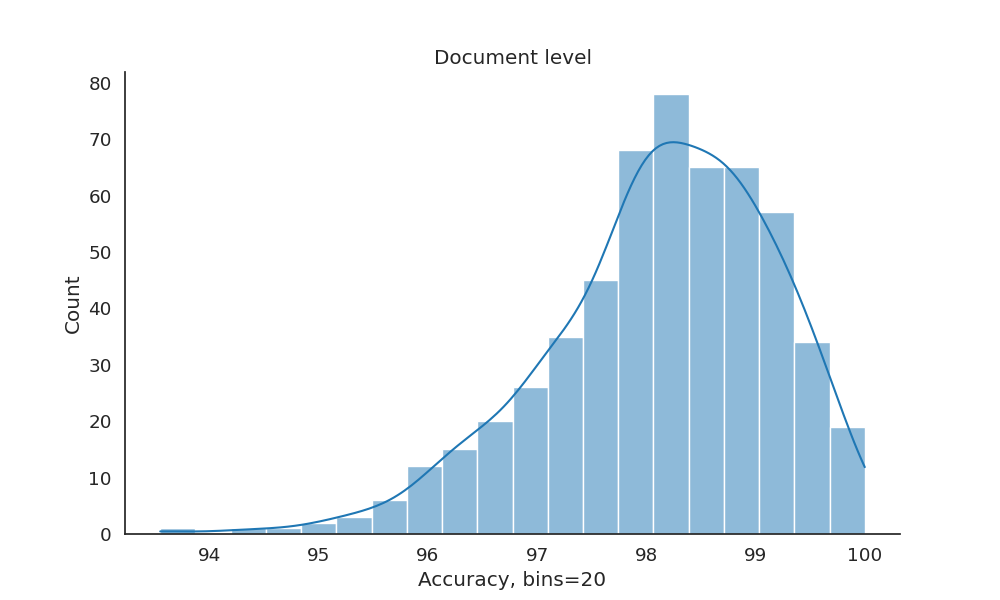
\includegraphics[width=\linewidth]{figures/err/accuracy-distibution-noweights.png}
	\end{minipage}
	\begin{minipage}[c]{0.45\linewidth}
		\centering
		Unweighted accuracy (140 docs)
		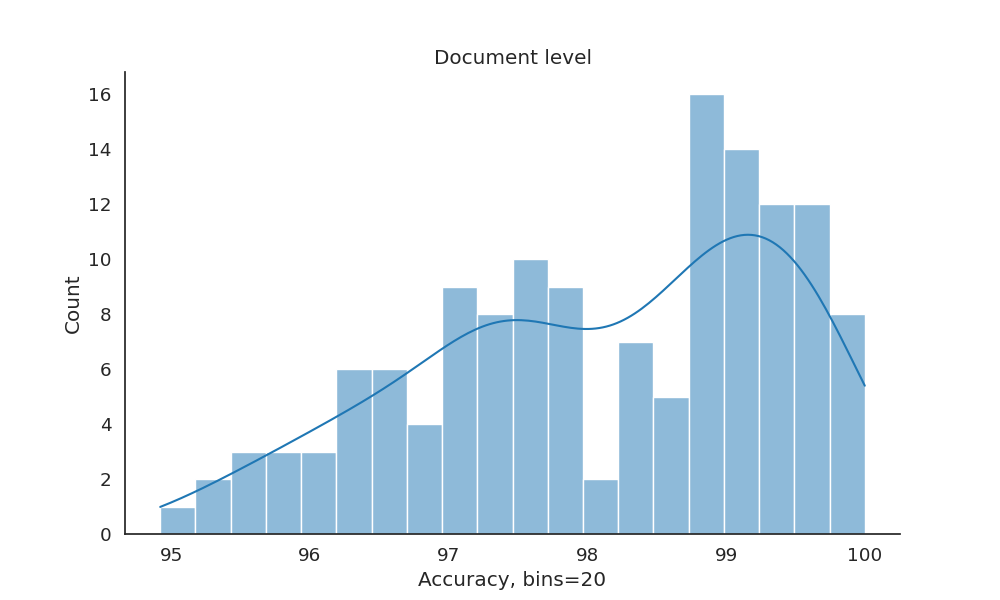
\includegraphics[width=\linewidth]{figures/err/accuracy-distibution-140.png}
	\end{minipage}	
	\caption{\label{fig:acc140binomial}Distributions of accuracy scores for error-annotated and cross-annotated datasets}	
\end{figure}

These details on data selection invalidate the differences in performance between accuracy and fluency on the cross-annotated dataset, while the observation about lack of difference between the two aspects from the point of view of all attempted representations stands. 
This conclusion was confirmed by \textbf{lack of statistical difference between accuracy and fluency} for all attempted representations on a random selection of 140 error-annotated documents. 
The results of this experiment are aggregated in Table~\ref{tab:err140rand_res}.

\begin{table}[H]
	\centering
	\begin{tabular}{l|cl|cl|cl|cl}
		\toprule
		& \multicolumn{2}{c|}{accuracy} & \multicolumn{2}{c|}{fluency}  & \multicolumn{2}{c|}{tq} & \multicolumn{2}{c}{scaled\_tq}    \\
		\midrule
		\multicolumn{9}{c}{Unweighted scores} \\
		\midrule
		& \textit{r}        & RMSE & \textit{r}       & RMSE & \textit{r}    & RMSE & \textit{r}    & RMSE  \\
		\midrule
		UD              & 0.2  & 1.11 & \textbf{0.36} & 1.02 & \textbf{0.36} & 1.72 & \textbf{0.34} & 14.8  \\
		all             & 0.28 & 1.08 & 0.25 & 1.04 & 0.3  & 1.74 & 0.27 & 14.9  \\
		quest61         & \textbf{0.29} & 1.09 & 0.29 & 1.03 & 0.28 & 1.77 & 0.26 & 14.94 \\
		\midrule
		tfidf           & 0.38 & 1.06 & 0.33 & 1.03 & 0.33 & 1.74 & 0.3  & 15.04 \\
%		\midrule
		TQmono-m        & 0.32 & 1.05 & 0.31 & 1.04 & 0.34 & 1.7  & 0.23 & 14.8  \\
		ruRoberta-large & 0.38 & 1.06 & 0.34 & 1.01 & 0.38 & 1.69 & 0.39 & 14.74 \\
		mdeberta3-base  & \boxit{0.3in}0.53 & 0.99 &\boxit{0.3in}0.45 & 0.95 & \boxit{0.3in}0.58 & 1.56 & \boxit{0.3in}0.54 & 14.6 \\
		\bottomrule
	\end{tabular}
	\caption{\label{tab:err140rand_res}Regression results for random 140 documents with error-based scores. For each quality score, the boldface type is used to denote the highest $r$ for manual features; the highest $r$ for content-dependent representations is boxed}
\end{table}

With regard to the \textbf{comparison between error-based and DA scores}, we have seen statistically significant results only for \textit{mdeberta3}, which returned higher results for accuracy, tq and scaled\_tq scores than for da\_zmean scores. 
All other comparisons were inconclusive. Interestingly, \textit{mdeberta3} was exceptional among all representations, including other embedding models. It returned stable and relatively high results regardless the type of error-based score, size of the dataset and distribution of scores. 

%UD features were statistically inferior to \textit{mdeberta3} only in the experiments for accuracy scores.

In sum, the experiments on an random selection of error-annotated documents confirmed \textbf{no difference in regression results for accuracy and fluency on any attempted representations} reported in Section~\ref{ssec:doc_err_res} (see Table~\ref{tab:doc_err_double}). 
We also \textbf{failed to obtain convincing proof that either error-based or DA scores were better aligned with the properties of translation} as represented in this work, except for \textit{mdeberta3} vectors that performed better on accuracy, tq and scaled\_tq scores than on da\_zmean scores. 

\paragraph{Feature analysis} 
We continue to trace the correlation of UD and QuEst++ features with the scores using feature selection and univariate tests, and limiting the analysis to the top ten most successful quality predictors according to both or either of these methods.
In this paragraph, we compared the set of features most associated with error-based scores to the set of features most correlated with DA scores. 

% scores: no statistically significant differences between results on full feature set and on selected features
Feature selection improved the results for \textit{da\_mean} on UD from 0.23 to 0.27 by limiting the feature set to just \textit{deverbals, nmod, nsubj}. The results on QuEst++ went up from 0.18 to 0.24 after limiting the feature set to 24 features. However, we forgo their analysis because the differences were not statistically significant.
%QuEST for da\_mean (24 fets r 0.18 -> 0.24) ['qe_1003', 'bqe_1009', 'qe_1011', 'bqe_1012', 'qe_1013', 'bqe_1015', 'qe_1018', 'qe_1024', 'qe_1028', 'qe_1034', 'bqe_1036', 'qe_1038', 'qe_1044', 'qe_1048', 'qe_1052', 'bqe_1054', 'qe_1055', 'bqe_1074', 'qe_1088', 'qe_1090', 'qe_1091', 'qe_1092', 'qe_1093', 'qe_9994']
\label{pg:da_ignores_translationese_feats}
The analysis of individual correlation of feature values and scores revealed \textbf{a noticeably different set of features correlated with DA scores than with error-based scores for UD and QuEst++}. 
In fact, there was only one UD feature that was in top ten by correlation with DA scores and with three error-based scores (\textit{nsubj}), while \textit{mark, neg, advcl} and \textit{sentlength} were shared with only accuracy or fluency, respectively.
None of these quality indicators support the translationese approach to quality, except, maybe, number of negations (\textit{neg}). If anything, these results mean that the longer and more complex the sentence, the higher the quality. In all likelihood, in \textbf{DA assessment setup translationese properties of texts were ignored by the raters}.  

UD features that were correlated with DA scores (but not with error-based scores) included \textit{mdd, aux, tempseq, aux:pass, mark, copula, advers}. They were positively correlated with DA scores. Higher MDD means higher comprehension difficulty, with sentences requiring additional effort for transforming longer linear distances into syntactic trees at understanding time~\cite[p.162]{Jing2015}. MDD values were greater in translations than in non-translated Russian, inviting a counter-intuitive conclusion that higher complexity correlated with higher quality. Increased frequencies of copula and auxiliary verbs, analytical passives are also signs of more noticeable translationese, which seems to be correlated with higher DA quality. The frequency of adversative discourse markers was negatively correlated with DA scores ($r=-0.224$), i.e. the more explicit markers of contrast were used in a translation, the lower was the perceived quality (e.g. \foreignlanguage{russian}{\textit{однако, несмотря на, тем не менее}} [however, despite, nonetheless]).
\textbf{These observations contradict our assumption that higher-quality translations should show less signs of translationese.}
% trade-off relation between the structural complexity in the two dimensions partially proves the dynamic balance of code-switching from the listener’s and speaker’s perspectives. English tends to reduce the structural complexity in the hierarchical dimension (MHD), while Czech prefers to lessen the processing cost in the linear dimension (MDD).

One common quality indicator among 61 QuEst++ features that cut across all types of quality scores (both DA and error-based) was \textit{the ratio of verbs in the source and target (\#1093)}. It was negatively correlated with the quality, i.e. the fewer verbs in the target, the higher the ratio, and the lower the quality. % which is contrary to what I think 
If anything, this observation contradicts the expectations in the context of English-to-Russian translationese tendencies as was the case with other results for translationese-aware features on error-based (see page~\ref{pg:scores_not_translationese}) and DA scores. Other DA predictors useful for accuracy and tq, or fluency were: 
% tq (\#1052, \#1085), fluency (\#1004)
\begin{description}\compresslist{}
	\item[1052] average bigram frequency in quartile 3 of frequency (lower frequency words) in the source corpus,
	\item[1085] ratio of percentage of content words in the source and target,
	\item[1004] number of tokens in the target over number of tokens in the source.
\end{description}
They were positively correlated with the respective quality scores. 

% discussed on page~\pageref{pg:quest_feats4err} 
Most correlative features that were specific for experiments on DA scores are listed below (in the decreasing order based on individual correlation with \textit{da\_mean} score): 
\begin{description}\compresslist{}
	\item[9992] ratio of word repetitions in target and source documents,
	\item[9993] ratio of lemma repetition between target and source documents,
	\item[1003] ratio of number of tokens in source and target,
	\item[1004] number of tokens in the target over number of tokens in the source,
	\item[1052] average bigram frequency in quartile 3 of frequency (lower frequency words) in the source corpus).
\end{description}

Interestingly, this list primarily includes adequacy features. Recall that error-based scores had ST complexity parameters as major quality predictors. 
Lack of intersection between error-based quality predictors and DA quality predictors from two interpretable feature sets make us conclude that these \textbf{types of assessment reflect dissimilar aspects of translation quality} or our feature sets are incomplete. 
Admittedly, this feature analysis has limited reliability, given weak association of any individual features with the DA scores (maximum $r=0.274$ for negative particles from UD feature set) and the general poor performance of any feature set on DA scores. 
However, the interpretation of most correlative features indicates that the \textbf{DA method does not reflect translationese properties of document}.
\vspace{-1.2em}

\subsection{\label{ssec:sent_level}Sentence Level: Error-based and DA Scores}
Given that error-based and DA scores originated at sentence level, we extended these experiments to the sentence-level version of the dataset. It included 3,224 sentences from 140 documents with error-based and DA scores. At sentence level, the distribution of scores was not as affected by the selection of a polarised smaller sample and remained heavily right-skewed for all scores as shown in Figure~\ref{fig:sents_tq} (page~\pageref{fig:sents_tq}). Nonetheless, we report results on randomly selected 3,224 sentences. The stack of experiments was run only for unweighted scores. For consistency, we present the results on the full dataset spanning 12,369 sentences, too.

At sentence level, there was enough data to establish that \textbf{translationese-aware features were relatively competitive only for fluency scores}. On the full dataset, they were outperformed for this type of quality only by \textit{ruRoberta} and \textit{mdeberta3}. For accuracy and tq, translationese-aware feature set was inferior to all other representations, including \textit{quest70} (a dedicated sentence-level QuEst++ feature set), \textit{tf-idf} and \textit{TQmono-m} in addition to \textit{ruRoberta} and \textit{mdeberta3}. This inferiority was lost on 3,224 sentences, except for \textit{ruRoberta} and \textit{mdeberta3}. It means that the differences in performance between UD, on the one hand, and \textit{quest70}, \textit{tf-idf} and \textit{TQmono-m}, on the other hand, were small. 

\label{pg:downward_slide}
The results for (unweighted) error-based scores at sentence level were generally almost twice lower than at document level for the full dataset of 553 documents/12,369 sentences (see Unweighted scores in Table~\ref{tab:doc_err_double}). For example, for fluency, UD features achieved $r=0.43$ at document level and $r=0.24$ at sentence level, while \textit{mdeberta3}'s results were $r=0.58$ and $r=0.36$, respectively. Manual frequency features were expected to be affected by sparsity. However, it is not clear why a dedicated sentence-level QuEst++ feature set and vectorised representations did not benefit from the shift from document to sentence level.

We noticed that the drop in performance caused by limiting the data to a (random) quarter of the original size was bigger for documents than for sentences. For example, the ratio of \textit{r} obtained from full/small document-level experiments for unweighted fluency on UD features was 1.19, while for sentence level it was 1.04. For \textit{quest70} these ratios were 1.44 vs 1.04, for \textit{ruRoberta} 1.56 vs 1.12 and for \textit{mdeberta3} 1.2 vs 1.09.
This means that at sentence level there was less volatility between the folds, and the learning process was more stable, even if not as successful as at document level, when enough data was available. 
%This also helps explain increased comatitiveness of \textit{ruRoberta} against \textit{mdeberta3}. The latter might be more robust to double mean-pooling to generate document vectors. 
These observations across many representations make us hypothesise that \textbf{error-based quality scores reflected the properties of texts better than they fit the properties of sentences}. 
\vspace{-1.5em}

\begin{table}[H]
	\centering
	\begin{tabular}{l|cl|cl|cl|cl}
		\toprule
		& \multicolumn{2}{c}{accuracy} & \multicolumn{2}{c}{fluency}  & \multicolumn{2}{c}{tq} & \multicolumn{2}{c}{scaled\_tq}    \\
		\midrule
		\multicolumn{9}{c}{Error-based scores (12,369 sentences)} \\
		\midrule
		& r        & RMSE & r       & RMSE & r    & RMSE & r    & RMSE  \\
		\midrule
		UD                & 0.21 & 3.91  & 0.24 & 4.7   & 0.21 & 3.91  & 0.2  & 11.97 \\
		all               & 0.21 & 3.91  & 0.26 & 4.67  & 0.21 & 3.91  & 0.21 & 11.97 \\
		quest70  & \textbf{0.24} & 3.93  & \textbf{0.26} & 4.67  & \textbf{0.24} & 3.93  & \textbf{0.23} & 11.96 \\
		\midrule
		tfidf             & 0.31 & 3.8   & 0.28 & 4.62  & 0.31 & 3.8   & 0.31 & 11.84 \\
%		\midrule
		TQmono-m          & 0.27 & 3.88  & 0.27 & 4.66  & 0.27 & 3.88  & 0.26 & 11.94 \\
		ruRoberta   & \boxit{0.4in}0.35 & 3.78  & 0.35 & 4.52  & \boxit{0.4in}0.35 & 3.78  & \boxit{0.4in}0.33 & 11.74 \\
		mdeberta3    & 0.32 & 3.82  & \boxit{0.4in}0.36 & 4.49  & 0.32 & 3.82  & 0.31 & 11.8  \\
		\midrule
%		\midrule
%		\multicolumn{9}{c}{Error-based scores (3,224 cross-annotated sentences)} \\
%		\midrule
%		UD              & 0.18 & 4.05  & 0.23 & 4.96  & 0.18 & 4.05  & 0.18 & 12.37 \\
%		all             & 0.17 & 4.05  & 0.23 & 4.95  & 0.17 & 4.05  & 0.17 & 12.38 \\
%		\textbf{quest70} & \textbf{0.19} & 4.07  & \textbf{0.24} & 4.93  & \textbf{0.19} & 4.07  & \textbf{0.19} & 12.38 \\
%		\midrule
%		tfidf           & 0.27 & 3.97  & 0.25 & 4.93  & 0.27 & 3.97  & 0.27 & 12.29 \\
%		\midrule
%		TQmono-m        & 0.25 & 4.03  & 0.27 & 4.93  & 0.25 & 4.03  & 0.25 & 12.35 \\
%		\textbf{ruRoberta} & \textbf{0.33} & 3.93  & 0.33 & 4.8   & \textbf{0.33} & 3.93  & \textbf{0.33} & 12.21 \\
%		mdeberta3  & 0.31 & 3.94  & \textbf{0.35} & 4.76  & 0tab:doc_err-da_corr.31 & 3.94  & 0.3  & 12.19 \\	
%		\midrule
		\multicolumn{9}{c}{Error-based scores (random 3,224 sentences)} \\
		\midrule
		UD              & \textbf{0.17} & 3.84 & 0.23 & 4.74 & \textbf{0.17} & 3.84 & \textbf{0.17} & 11.77 \\
		all             & 0.17 & 3.84 & 0.24 & 4.71 & 0.17 & 3.84 & 0.17 & 11.77 \\
		quest70         & 0.14 & 3.87 & \textbf{0.25} & 4.7  & 0.14 & 3.87 & 0.13 & 11.79 \\
		\midrule
		tfidf           & 0.21 & 3.77 & 0.22 & 4.73 & 0.21 & 3.77 & 0.21 & 11.69 \\
%		\midrule
		TQmono-m        & 0.21 & 3.83 & 0.24 & 4.72 & 0.21 & 3.83 & 0.21 & 11.75 \\
		ruRoberta & \boxit{0.4in}0.29 & 3.75 & 0.31 & 4.6  & \boxit{0.4in}0.29 & 3.75 & \boxit{0.4in}0.29 & 11.63 \\
		mdeberta3  & 0.27 & 3.77 & \boxit{0.4in}0.33 & 4.56 & 0.27 & 3.77 & 0.27 & 11.66 \\
		\bottomrule
	\end{tabular}
	\caption{\label{tab:sent_err_double}Sentence-level results for unweighted error-based scores. For each quality score, the boldface type is used to denote the highest $r$ for manual features; the highest $r$ for content-dependent representations is boxed}
\end{table}

% where is my answer to the main question? How good are UD features for predicting sentence-level scores from errors and from DA? 

Sentence-level experiments, contrary to document-level, \textit{yielded evidence that fluency scores were more learnable than accuracy scores}, at least, on UD and \textit{mdeberta3} for both full and reduced datasets (see Table~\ref{tab:sent_err_double}). 
This is an expected and comforting outcome which provides circumstantial evidence of error annotation validity and of the distinctions between the accuracy and fluency in principle when enough data is available. At the same time, for the practical purposes of human translation quality estimation, these distinctions are negligibly small. 

To cross-examine our conclusion from document level that neither error-based nor DA scores were better aligned with the properties of translation than the other, we obtained the results for DA at sentence level. 

Spearman's \textit{r} between rater1 and rater2 on sentence-level DA scores was 0.408 (p < 0.05). This was a bit lower than for document-level perspective ($r=0.503$). To give more details on the parameters of the cross-annotated sentence-level variant of the dataset, the correlation between error-based scores and DA is reported in Table~\ref{tab:sent_err-da_corr}, measured with Spearman's $r$. Correlation between two assessment methods at sentence-level was much lower than at document level (cf. Table~\ref{tab:doc_err-da_corr}, page~\pageref{tab:doc_err-da_corr}).

\begin{table}[H]
	\centering
	\begin{tabular}{l|ccc|ccc}
		\toprule
		& \multicolumn{3}{c|}{unweighted} & \multicolumn{3}{c}{weighted} \\
		\midrule
		& accuracy   & fluency & tq    & accuracy & fluency & tq    \\
		\midrule
		da\_mean & 0.291 & 0.149 & 0.291 & 0.311 & 0.165 & 0.33 \\
		\bottomrule
	\end{tabular}
	\caption{\label{tab:sent_err-da_corr}Sentence-level: Spearman's $r$ between averaged DA scores and each of the error-based scores}
\end{table}

Table~\ref{tab:da_sent_res} presents the results for DA scores on sentence-level version of the dataset. 
% how did UD perform against other reps?? 
With regard to the main question of this thesis -- whether translationese-aware UD features were competitive against other representations in predicting quality -- the results for DA scores demonstrated that they were inferior to \textit{ruRoberta} and \textit{mdeberta3} as before, but also to \textit{TQmono-m}. Note that \textit{TQmono-m} was specifically trained for predicting this type of quality -- DA scores -- on MT data. 
\label{pg:no_slide_for_da_when_moving_to_sent}
Sentence-level results for DA scores were better than at document-level on all representations, but especially for QuEst++ (cf. da\_mean: $r=0.33$ vs $r=0.18$) and \textit{ruRoberta} ($r=0.39$ vs $r=0.22$). Curiously, this was not the case with error-based scores where we discussed a unanimous downward slide on all representations (see page~\pageref{pg:downward_slide}). 
This emphasises the differences between the two manual assessment methods. \textbf{Document-level translation quality scores can be produced more reliably using error annotation than DA setup}. 
\begin{table}[H]
	\centering
	\begin{tabular}{l|cl|cl}
		\toprule
		           & da\_mean &      & da\_zmean &      \\
		\midrule
		               & r         & RMSE & r          & RMSE \\
		\midrule
%		\multicolumn{5}{c}{2raters}     \\ 
%		\midrule
		UD              & 0.29 & 12.89 & 0.29 & 0.84 \\
		all             & 0.3  & 12.86 & 0.3  & 0.83 \\
		quest70         & \textbf{0.33} & 12.74 & \textbf{0.33} & 0.82 \\
		\midrule
		tfidf           & 0.27 & 12.94 & 0.31 & 0.82 \\
%		\midrule
		TQmono-m        & 0.35 & 12.56 & 0.37 & 0.81 \\
		ruRoberta & \boxit{0.4in}0.39 & 12.41 & \boxit{0.4in}0.42 & 0.78 \\
		mdeberta3  & 0.39 & 12.45 & 0.38 & 0.80 \\
		\bottomrule
	\end{tabular}
	\caption{\label{tab:da_sent_res}Sentence-level: Regression results for DA scores by SVR. The highest result for manually engineered feature sets is shown in bold; the highest result for content-dependent classifiers appears in a box}
\end{table}

% \textbf{Error annotation (as implemented in the \gls{RusLTC}, see Section~\ref{ssec:err}, page~\pageref{ssec:err}) is more fit to produce document-level scores than DA setup}. 

%\textit{mdeberta3} did not match the other representations in the scale of gain when moving to sentence level for this type of score. It seems to be performing better at document level.

At document level, there was no evidence that either error-based scores or DA scores returned higher results on any representations, except marginal superiority for accuracy and tq over DA on \textit{mdeberta3} (see page~\pageref{tab:err140rand_res}).

Sentence-level experiments provide ample evidence that \textbf{DA scores were more learnable than any error-based scores, given the same sample size}. In fact, the experiments on sentences from the same 140 cross-annotated documents and on a random sample of 3,224 sentences returned results that were higher for DA scores than for error-based scores on an overwhelming majority of representations. 
For example, UD results was $r=0.29$ for da\_mean score and $r=0.23$ for fluency on random 3,224 sentences; \textit{mdeberta3} returned $r=0.39$ for da\_mean score and $r=0.33$ for fluency.

We leave out feature analysis at sentence level for two reasons. First, we believe that translationese is primarily a document-level property. Second, UD features are heavily affected by sparsity in this setting. 

\section{\label{sec:qua_disc}Discussion}
% overview
This chapter evaluates the ability of linguistically-motivated translationese indicators to predict professional varieties and human translation quality against alternative document representations and with regard to various methods to generate quality judgments. 

The performance of ML algorithms on hand-engineered translationese features was contrasted with the results on document-level features from QuEst++, a MT quality estimation framework, on \textit{tf-idf} representation, and on vectors from two types of embeddings: cross-lingual sentence embeddings and word embedding (a large dedicate TL (Russian) model and the most recent multilingual SOTA in representation learning).

We evaluated the ability of our representations to distinguish between student and professional translations viewed in this work as a possible proxy for translationese-related quality.
In quality estimation tasks, we explored the learnability of three types of quality judgments, including (i) binary quality labels from holistic document-level assessment of translations, (ii) continuous quality scores generated from error annotation and (iii) continuous quality scores from sentence-level DA annotation. 

\paragraph{Translationese indicators for translation varieties and `good/bad' translations}  % binary quality
The classification experiments to distinguish professional and student translations demonstrated that the differences between them were only marginally related to translationese. The weak signal picked by translationese indicators was overshadowed by other (semantic and functional) dissimilarities between the two parallel corpora. This limitation of our setup was anticipated, and measures were taken to obtain most comparable subsets from a much larger corpus resource (see Section~\ref{ssec:mypro}, page~\pageref{pg:stu_pro_made_comparable}).
We found that in this experiment QuEst++ significantly outperformed all other hand-engineered feature sets, reaching $F1=86.17$ after feature selection. The success of the feature set was explained by the performance of complexity features that captured the diverging properties of the STs in the two parallel corpora. 

Our representations did not target accuracy specifically. The only feature set that implicitly compared ST and TT to access relations between them was QuEst++. It did not perform well on any task targeting quality labels or scores. Therefore, we omitted feature analysis for those tasks.

On the varieties dataset, QuEst++ feature set performed well but it relied on ST-related components that in our setting could not be reliably interpreted as quality indicators. 
The selection of well-performing QuEst++ features that did not depend entirely on the properties of ST was limited to several fluency features and three adequacy features. QuEst++ fluency features confirmed that student translations were more perplexing to a TL model than professional translations. Student translations used a greater ratio of n-grams unseen in non-translations. The three adequacy features demonstrated that student translations were less wordy but more repetitive than professional translations (see page~\pageref{pg:quest_adequacy_feats_for_vars}).

The best-performing UD subset of 15 features achieved $F1=79.39$ on this task. This subset included only six features that were also strong translationese predictors, mostly reflecting the syntactic complexity of target sentences (number of clauses, clausal complements and subordinating conjunctions). On these features student translations were simpler and closer to the reference corpus than professional translations although the differences between the document categories were small. On other translationese features, contributing to the varieties distinction, students demonstrated stronger translationese tendencies due to underuse of negation, overuse of copula verbs and relative clauses but we did not have enough data to obtain statistical evidence for those observations. 

The most prominent quality indicators from UD features did not have strong association with the labels, maximising at the level of 0.34 for \textit{parataxis} (measured as F1-score from a single-feature classifier). Comparative analysis for this feature demonstrated that students preferred to use explicit markers of cohesion, which led to a lack of asyndetically introduced elements. This makes student translations most distinct from professional translations, and especially from non-translations.
Professionals clearly avoid using analitical passives, a quite legitimate grammatical form in Russian, which might be associated with the perception of passive as unwanted shining-through effect in English-to-Russian translation education. This leads to a conspicuous lack of analytical passive forms in the professional subcorpus. 
%%%%%%%%%

\textbf{Translation quality classification} proved to be an even more challenging task for all representations. First, there was little content variation between the categories because good and bad translations were produced from the same 57 English STs. Second, the quality-labelled dataset was almost twice smaller than the professionalism dataset (708 vs 360 instances). % 

Despite these limitations, UD features were much more successful in this task, demonstrating that the \textbf{amount of translationese is well-correlated with the document-level quality assessment}. 

\label{pg:translationese_indicators_work_for_binary_labels}
Linguistically-motivated translationese-aware features were inferior only to \textit{ruRoberta} and \textit{mdeberta3}, large pre-trained contextualised word embedding models. Unlike in the other experiments, RFECV feature selection offered a significant gain in performance, bringing our classification result on UD features to $F1=68.9$ (vs $F1=78.14$ on \textit{mdeberta3}).

We argue that a reasonably good performance of out-of-the-box contextualised word embeddings on this dataset indicates that human assessment of quality at document-level is actually related to the objective properties of the texts (even if not enlightening), and might not be as subjective as it is common to believe in MT (see our discussion on page~\pageref{pg:pessimism}), at least, when it is trusted to translation professionals. 

The results of feature analysis suggest that quality distinctions were much more related to translationese than differences between professional varieties of translation. 
We demonstrated that there were only three (out of 26) quality predictors that were not among translationese indicators. Professionalism turned out to be a more vague concept than quality, at least from the point of view of translationese indicators.

An explanatory analysis of translational trends in \textit{bad} translations demonstrated that \textbf{lower quality was associated with the lack of ability to recognise and counteract the ST influence} to a considerable extent. For the features, where there was enough evidence to establish differences between \textit{good} and \textit{bad} translations, we observed translationese trends which implied passively following ST patterns, with little or no effort to adapt them to the TL norm.
 
Generally, lower-ranking translations were found further away from non-translations in Russian than higher-ranking translations for the same STs across most analysed features.  
%%%%%%%%%%%%%%%%%%%%%%%%%%%% 31 October, 1 Novermber still here %%%%%%%%%%%%%%%%%%%%%%%
\paragraph{Translationese indicators and continuous quality scores}
Sections~\ref{ssec:doc_err_res},~\ref{ssec:doc_da_res} and~\ref{ssec:sent_level} reported the experiments to predict quality scores generated from error annotation and in DA setup. Our focus remains on evaluating the performance of translationese indicators against other representations, and on explaining the findings using interpretable features.

Importantly, scores from error-annotation allow to disintegrate translation quality into accuracy and fluency, and test whether fluency returns higher results on the representations that have access to the TL-side of the corpus only. 
Besides, scores offer an opportunity to extend document-level experiments to sentence level. On the one hand, this allows to alleviate the problem of small training data at document level. On the other hand, it helps uncover important properties of scores generated by each assessment method.

Section~\ref{sec:_scores} brought together several aspects of this multi-faceted comparison, namely, experimental results are compared across:

\begin{itemize}\compresslist{}
	\item seven representations, focused on comparative performance of UD features,
	\item various scores and their versions from two manual assessment methods, including on a cross-annotated subset,
	\item most successful features from hand-engineered sets.
\end{itemize}

We have seen that the outcomes of these comparisons were largely dependent on the level of analysis: document or sentence.

\paragraph{1. Translationese-aware features vs. contextualised embeddings}
%\pageref{pg:doc_err_ud_vs_all} %Performance of UD against other representation
Our major hypothesis was that translation quality (calculated from error statistics or perceived in DA setting) can be captured by looking at the amount of translationese in a translation. 

Cross-lingual, dedicated Russian and multi-lingual embedding models (\textit{TQmono-m, ruRoberta, mdeberta3}, respectively) were comparable to the proposed hand-engineered translationese-aware feature sets in that they did not recur to the source text and encoded the properties of the target side of the dataset only.

Table~\ref{tab:_ud_vs_all} summarises the outcomes of all experiments showing the models that were statistically superior to UD. It uses unweighted versions of error-based scores and results on random 140/3,224 error-annotated instances.

\textbf{For document-level scores, linguistically-motivated translationese features returned compatible performance against other representations}. As can be seen from Table~\ref{tab:_ud_vs_all}, they were statistically surpassed only by \textit{mdeberta3}, the most recent embedding approach and current SOTA in NLP representation learning, in all experiments on both error-based and DA scores. Admittedly, the performance on document-level DA scores and on random 140 error-annotated documents was very poor due to the size of the dataset, and no statistically significant differences were seen between any two representation. 
%This renders most of our observations anecdotal and less unreliable than expected. 
Lack of a bigger annotated data prevents us from attempting any fine-tuning methods, especially for DA-annotated dataset.

\begin{table}[H]
	\centering
	\begin{tabular}{l|p{2cm}c||p{3cm}p{3cm}}
		\toprule
		& \multicolumn{2}{c||}{Document level} & \multicolumn{2}{c}{Sentence level} \\
		\midrule
		& 553 docs & 140 docs   & 12,369 sents & 3,224 sents  \\
		\midrule
		accuracy   & mdeberta3 & mdeberta3 & all reps & ruRoberta mdeberta3 \\
		fluency    & ruRoberta mdeberta3 & -- & ruRoberta mdeberta3 & ruRoberta mdeberta3 \\
		tq         & mdeberta3 & -- & all reps & ruRoberta mdeberta3 \\
		%		scaled\_tq & ruRoberta mdeberta3 & mdeberta3 & ruRoberta mdeberta3 & mdeberta3 \\
		\midrule
		da\_mean   & NA & -- & NA & TQmono-m ruRoberta mdeberta3 \\
		da\_zmean  & NA & -- & NA & TQmono-m ruRoberta mdeberta3 \\
		\bottomrule
	\end{tabular}
	\caption{\label{tab:_ud_vs_all}Representation superior to translationese-aware UD on quality scores}
\end{table}

\textbf{At sentence level} on all available error-annotated instances (12,369), \textbf{UD features performed well on fluency scores only}, being secondary to two word embedding models. For accuracy and overall translation quality, UD features were not competitive (they were outperformed by all other representations). This outcome makes sense: if accuracy reflected semantic similarity between ST and TT, translationese indicators should not be able to predict this type of quality. However, the differences in performance between various representations were very small. They were picked on a large annotated dataset only. They went away if not enough data was available (cf. sentence-level results on 12K and 3K observations in last column in Table~\ref{tab:_ud_vs_all}).

For sentence-level DA scores translationese-aware features were inferior to \textit{ruRoberta} and \textit{mdeberta3} as before, but also to \textit{TQmono-m}, a model optimised to predict DA scores on MT data. This observation might mean that \textbf{DA scores have specific properties shared between MT dataset and HT dataset} built for the purposes of this research. 

Although direct comparisons with any previous work on document-level automatic human translation quality estimation is problematic, we can compare our results to those reported by~\citet{Yuan2018}. % 457 multiple student translations, counting 3,569 sentences
They reported Pearson's $r=0.72$ against \textit{QuEst++} baseline result of $r=0.67$ for the best-performing subset of their manual features on document-level English-to-Chinese dataset based on overall quality (for more details see our description of their work on page~\pageref{pg:yuan_previous}). % see Table 6.9 at p 138 in their thesis
We obtained the highest Spearman's $r=0.45$ on UD features for overall quality, with QuEst++ features returning $r=0.36$ (the difference is not statistically significant). The absolute best result on our dataset is $r=0.67$ (\textit{mdeberta3}). This comparison demonstrates that in relative terms our features offered a comparable increase on the QuEst++ baseline for our dataset. % which was more fair than the one explored by Yuan 2018.

%We recalculated the results in Table~\ref{tab:doc_err_double} for Pearson's correlation in our setting and obtained the highest result of $r=0.45$ on UD features for overall quality, with QuEst++ features returning $r=0.44$ (the difference is not statistically significant). The absolute best result on our dataset is $r=0.64$ (\textit{mdeberta3}).
% was not significantly different from QuEst++ performance of $r=0.44$ on the best-performing subset of 31 features.   

\paragraph{2. Error-based scores vs. DA}
Our experiments put under scrutiny 10 continuous quality scores and their versions from two annotation methods.
In general, it seems that no modification of raw scores was able to yield better results across all representations than their raw counterparts. If anything, they performed worse. This applies to weighted error-based scores, scaled overall quality from error annotation (scaled\_tq) and to z-transformed DA scores (da\_mean).

Another important comparative conclusion about various scores is that \textbf{error-based scores seem to capture document-level properties better than DA scores, but DA scores are superior for sentence-level experiments}. 
Although in both annotation scenarios annotators were exposed to the entire documents, while providing judgments on the properties of individual sentences, error-based scores were more learnable than DA scores at document level than at sentence level (including on the dataset of the same size). We have shown that unlike DA scores, error-based scores demonstrated a considerable decrease in performance when moving from document level to sentence level on the same dataset (see pages~\pageref{pg:downward_slide} and~\pageref{pg:no_slide_for_da_when_moving_to_sent}). 
Document-level nature of error-based scores is further supported by a bigger drop in their performance for documents than for sentences when moving from full dataset (553 documents/12,369 sentences) to random forth of the data (140 documents/3,224 sentences). The sentence-level performance of error-based scores was poor at the full dataset, so it did not suffer as great a tumble on limited data.
% five separate speculations!
Finally, we made an interesting observation about the relations between accuracy and fluency, the two major theoretical aspects of quality, which stir a lot of controversy in the literature on benchmarking translation quality by humans (see our discussion on page~\pageref{pg:controvercy_over_acc_and_flu}).
According to our results, the difference between accuracy and fluency was visible only at sentence level and only for some representations. In particular, only UD and \textit{mdeberta3} returned expected statistically higher results for fluency than for accuracy on both full and reduced datasets. % QuEst++ also had statistically higher results for fluency but ONLY on random 3224, and surprising, not on the large dataset
At document level, there was no evidence that either accuracy or fluency was more aligned with the properties of documents picked by any attempted representations. 
This lack of evidence at document level can be explained by the lack of training data. 
However, our experiments were run on 553 annotated translations. If more data is needed to see the differences between the two, then the difference must be really small. Another explanation is that error-based judgments capture local issues in translations and should not be used to generate overall quality scores, especially across all sentences in a document. Finally, we can hypothesise that, in line with the assumption made in this thesis, accuracy errors indeed introduce disfluencies in human translation, and therefore, scores based on content errors can be learnt using representations that do not have access to ST (such as UD which achieved $r=0.427$ and \textit{ruRoberta} with $r=0.534$ at document-level).
With regard to UD representation, especially given its relatively low result, another plausible explanation is that \textbf{scores from error annotation do not reflect translationese properties of translations, at least when they are generated for entire documents}. It is quite possible that errors were focused on other, more localised, imperfections of student translations, instead of translationese. It stands to reason, because translationese is in essence a `distributed' statistical property of translation which is difficult to put a finger on in individual sentence in error annotation.
A more general interpretation of this outcome, which also incorporated \textit{mdeberta3} performance, can be that the \textbf{distinction between accuracy and fluency is negligibly small for all practical purposes of quality estimation at document level}.

The relation between scores from the two assessment methods provide an important insight on the nature of human perception of translation quality in DA setting. We showed that (i) accuracy was almost four times more correlated with DA scores than fluency; (ii) weights increased this correlation and (iii) weighted overall quality returned the highest correlation with DA scores, which reached $r=0.559$ (see Table~\ref{tab:doc_err-da_corr}). Professional human raters in both annotation schemes laid greater emphasis on accuracy. 
% Humans tend to agree on accuracy more, while machines are better at predicting fluency, if this distinction is made at all. 
At the same time, most attempted representations, including those that were not focused on translationese-related fluency and could pick up the signal coming from the ST directly (QuEst++) or indirectly (\textit{TQmono-m}, \textit{mdeberta3}), had a tendency to return higher results for fluency or tq, especially on smaller datasets. It means that machines struggle with picking those aspects of quality that are deemed more important by humans, namely accuracy and adequacy. Arguably, fluency is the least `non-binary' aspect of translation quality. Unlike accuracy, it does not rely too much on human understanding and interpretation of language, context or cross-linguistic correspondences. 
%It is also noteworthy that the comparison of two manual annotation schemes on our sample suggests that the semantic accuracy component of quality is not as subjective as it is commonly believed. The two types of annotation schemes achieve reasonably high agreement of Spearman's $r=0.509$ between DA scores and weighted accuracy. For weighted overall quality scores the correlation was even higher (Spearman's $r=0.559$).

\paragraph{3. Feature analysis results by score type}
In the regression experiments, the feature selection process and univariate feature analysis proved less enlightening than in classification tasks. It was limited to the document-level scores only.

We have seen but very modest improvements in regressor performance, if any, on feature selections returned by \gls{RFECV} (setup with a linear kernel, $C=1.0$ and Spearman's r as a scoring function).  

Similar to~\citet{Yuan2018}, we found that the strongest quality indicators were well-associated with all error-based quality scores (three most correlated UD features and top six QuEst++ features out of 10). 
This supports the opinion that accuracy and fluency are but artificial constructs which are difficult to tease apart objectively. % in practical terms. 

We also observed that the features most correlated error-based and DA scores were quite different. There was one `universal' quality indicator in the selections of 10 most effective UD and QuEst++ features that was also well-associated with the other type of quality scores. They were \hyperlink{ft:nsubj}{number of nominal subjects} and \textit{ratio of verbs in the source and target} (1093), negatively-correlated with all quality scores.

We can hypothesise that error-based and DA scores captured dissimilar parameters of translation quality. A bit larger intersection between good DA and good accuracy indicators confirms that raters who were tasked with perceived quality annotation gave more weight to distortions in semantic relations between ST and TT than to imperfections in linguistic expression.

With regard to the relation between the amount of translationese and quality scores, we have to conclude that \textbf{error annotation and, especially DA, largely ignore translationese properties of translations}. 
At document level, where the relation between translationese and quality was expected, scores from these assessment methods returned correlations with translationese indicators that partially contradicted the expectations based on translationese perspective of quality. 
Contrary to what we observed on binary quality labels from holistic assessment of translations (see discussion on page~\pageref{pg:translationese_indicators_work_for_binary_labels}), feature analysis in experiments with quality scores did not reveal a consistent link between translationese properties of documents and their quality. 
If anything, the interpretation of many linguistic features from UD and QuEst++ feature sets resulted in a counter-intuitive conclusion that more translationese was correlated with higher quality, especially for DA scores (see analysis on pages~\pageref{pg:scores_not_translationese} and~\pageref{pg:da_ignores_translationese_feats}).

In a broader perspective, this research demonstrated the benefits of linguistically-motivated features for understanding the differences between translation-quality related categories of documents, and revealed the contrastive properties of three quality assessment methods. Feature-based approaches are useful for understanding the performance of contextualised embeddings. 
The most immediate use of the proposed method is segregating new multiple translations of a source text into `good' and `bad' by measuring distances between vectors of translated texts and an averaged vector representing the expected TL norm. 
A similar methodology can be used to identify documents produced by language learners and, probably, estimate the level of foreign language competence, complete with the explanation of deviations typical of cohorts with various mother tongues. It is potentially applicable for distinguishing documents produced by students and by automatic language generating applications such as chatbots. 

%\include{chapters/6_sentence}
\chapter{\label{cha:fin}Conclusion}
%\todo[inline]{An suggests that chapters should start on odd page}
This thesis applies ideas from translationese studies to human translation quality estimation. 
Using machine learning methods, it explores the extent to which translationese properties of text can explain the quality judgments obtained by holistic assessment of translated documents, error annotation and direct assessment of sentences in context. Additionally, we use professional and student translations as ontological varieties that can be related to quality. 

The investigation has an explanatory focus. It employs linguistically-motivated features to discern patterns in translational behaviour and individual types of translation solutions that can be associated with lack of professionalism or lower translation quality. Our findings contribute to translationese studies and are applicable in translation education. 
Besides, the thesis offers a comprehensive comparative study of translation quality assessment methods, including those used to benchmark translation quality in machine translation. It sheds light on the important properties of quality labels and scores originating from various approaches to manual quality assessment. 

The hypothesis that translationese properties are related to translation quality will be supported, if it can be shown that strong translationese indicators are also well-correlated with translation quality labels and scores, and/or that translationese-related phenomena are more expressed in lower quality translations. For example, \citet[][p.357]{Hu2021} conclude their multilingual translationese study by stating: ``translations tend to have more relative clauses. This seems to be truly universal despite obvious differences in the source languages''. If they are right, normalised frequency of relative clauses in a translated document should be among strong translation predictors for English-Russian language pair. Further on, if our hypothesis stands, relative clauses should be on the list of strong quality predictors and/or be relatively well-correlated with the quality labels and scores. 

The relation between translationese and quality has been suggested in the literature many times (see Section~\ref{sec:feats4qua}). However, we are not aware of research that would put this proposition to an empirical test by machine learning methods, at least, for human translations. This thesis frames the problem as a human translation quality estimation task supported by statistical testing and feature analysis. Our major focus is on document-level quality, which is known to be under-researched in MTQE, including due to lack of annotated data and limitations of representation learning. Importantly, our hypothesis makes us rely on predicting quality using the target language side of the parallel corpora, while ignoring the relation between ST and TT. We contend that in human translations produced in good faith, deviations from semantic similarity between ST and TT would usually distort the natural flow of text and create weird nonsensical renditions suggestive of accuracy errors. 

The aim and the methodology of this research place it at the interface of a number of disciplines. It builds on the knowledge and findings in: 
\begin{itemize}\compresslist{}
	\item translation studies, especially in the areas of translationese studies, \gls*{TQA}, professional competence research and pedagogy,
	\item corpus linguistics, especially building learner and parallel corpora and corpus analysis methods, 
	\item \gls*{MTQE}, and applications to HTQE,
	\item \gls*{ML} and \gls*{NLP} for computational methodology.
\end{itemize}

\section{Contributions}
%\todo[inline]{An suggests that there should be more cross-referencing in contributions, like page ranges}
Our contributions can be summarised as follows: % they span several research areas
\begin{enumerate}\compresslist{}
	\item \textit{We designed and rigorously tested three sets of linguistically-motivated translationese indicators for English-Russian translations of mass-media texts}. 
	
	They include 60 morphosyntactic features extracted from Universal Dependencies annotation and two smaller sets of abstract lexical features, including 24 collocational features and 11 features from n-gram language models. The selection process was guided by translation theory as well as by findings from previous empirical studies. In particular, these features include most translationese indicators from a comprehensive set developed by~\citet{Volansky2015}, which is used as a baseline in many translationese studies. With regard to the UD features, care was taken to include only cross-linguistically comparable isomorphic features informed by the contrastive analysis of English and Russian that could hypothetically pick specificity of language choices in the situation of translation (Section~\ref{sec:myfeats}). 
	
	Our experimental results on two independent collections of translations proved that structural morphosyntactic features were by far more effective in distinguishing translations and non-translations. They were also very competitive against vector representations from pre-trained contextualised embedding models, including a dedicated Russian language model and a multilingual \textit{mdeberta3}, the current SOTA in generic representation learning (Section~\ref{sec:detect}).      
	
	\item \textit{We identified most prominent translationese indicators for English-Russian mass-media translation, associated with `shining-through' trend in translational behaviour, using bottom-up approach}. 
	
	Multivariate analysis through feature selection revealed a large intersection between sets of translationese features that were most effective in predicting student or professional translations against non-translations. In univariate analysis, these translation varieties were shown to exhibit similar trends in translational behaviour along the same dimensions of analysis, most notably, `shining-through'.
	
	The most prominent translationese indicators were among syntactic, rather than morphological, features, and signalled a tendency to produce longer and more complex sentences in translation. We confirmed some of the translational distortions anticipated by translation theory and practical textbooks on English-to-Russian translation. Namely, frequencies of the following items tend to be higher in translations than in non-translations: additive discourse markers, analytical passives, copula verbs, modal predicates, personal pronouns, finite verbs and determiners.
	The explorations at the lexical level indicated that translations were likely to have more of unusual strings, unseen in a large TL model. They relied on a smaller variety of collocations, and the collocation in translations were less familiar to the language model (Section~\ref{sec:bestof}). % had lower association score 
	
	\item \textit{We obtained evidence that differences between translations produced by student and professional translators were much less related to translationese than distinctions between \textit{good} and \textit{bad} translations.} %However, a clear distinction among them can be to an extent interpreted as related to quality.
	
	Translationese-aware UD feature set was outperformed on this classification task by QuEst++ features. Despite QuEst++ success can be largely explained by differences in the STs, findings on prominent fluency and adequacy features demonstrated that student translations were more perplexing to a LM trained on non-translations, most likely due to `strange strings' and awkward word choices. Student translations were also found more repetitive. Analysis of a few strong translationese indicators, selected as predictive of student/professional class, returned contradictory results. Some expected translational behaviours were actually more noticeable in professional translations, while other -- in student translations. For example, professional translations were found to contain longer sentences, more epistemic markers and modal predicates than student translations. However, on other translationese features, professionals demonstrated more ability to recognise and counteract known translationese trends (more indirect objects and negative particles, fewer analytical passives).
	Besides, the association between translationese features and labels was very low, with many strong translationese predictors being irrelevant for student/professional classification (Section~\ref{sec:labels}).
	
	\item \textit{We provided evidence that prominent translationese indicators were indeed predictive of document-level quality labels from holistic assessment confirming that the amount of translationese was well-associated with human perception of translation quality.}   
	
	Linguistically-motivated morphosyntactic translationese features were competitive against other representations on document-level quality labels. They outperformed QuEst++ and were second only large pre-trained word embedding models. Feature analysis provided further overwhelming support for our hypothesis that translationese indicators can be useful in predicting quality. Note that this finding was limited to holistic assessment of document-level quality. We demonstrated that, in the experiment on binary quality labels, lower-ranking translations were always more distant from the expected target language norm and were well-associated with stronger translationese trends (Section~\ref{ssec:bin})
	
	\item \textit{We demonstrated that quality judgments from three assessment methods revealed dissimilar properties: they accounted for translationese to various extents and performed better at document or sentence level.} 
	
	Quality scores derived from error annotation and from sentence-level direct assessment were shown to be less translationese-aware than document-level holistic perception. The study of association between translationese indicators and error-based scores returned ambiguous results. Some results were coherent with translationese approach to quality (the higher the score, the less translationese), while for some features higher-scoring translations manifested more translationese.
	Comparative performance of various representations demonstrated that error-based scores returned higher results at document level, while scores from direct assessment performed better at sentence level. % (i) dedicated sentence-level QuEst++ feature set and vectorised representations did not benefit from the shift from document to sentence level. (ii) the drop in performance caused by limiting the data to a (random) forth of the original size was bigger for documents than for sentences. (iii) DA returned higher results than any error-based scores on same-size sentence-level dataset (iv) Sentence-level results for DA scores were better than at document-level on all representations, but especially for QuEst++ (cf. da\_mean: $r=0.33$ vs $r=0.18$) and \textit{ruRoberta} ($r=0.39$ vs $r=0.22$). Curiously, this was not the case with error-based scores where we discussed a unanimous downward slide on all representations (see page~\pageref{pg:downward_slide}). 
	Additionally, in our setting there was no evidence that any attempted document-level representations returned better results for accuracy or fluency. Given that some of our representations did not have direct or indirect access to the SL, this outcome raises doubts about the practical reliability of this distinction, at least, at the document level (Sections~\ref{ssec:bin} and~\ref{sec:_scores}). 
	
	\item \textit{We release relatively large document- and sentence-level aligned datasets based on student translations with holistic document-level labels, error-based and DA scores that can be used for \gls{HTQE}}.
	% RusLTC-HTQE-binary rusltc-htqe-binary rusltc-htqe-scores
	The datasets contain English-to-Russian translations of mass-media texts from the \textit{RusLTC} and were produced by senior students majoring in translation at BA or MA (specialist) levels. 
	Documents with binary labels (360 documents) include several top and several bottom translations to 57 English texts that were offered to students as test assignments or translation competition tasks. Multiple translations to each ST were sorted by the final grade (agreed between jurors/examiners) that was returned to students or announced at a competition.
	Error-based scores are frequencies of translation errors normalised to the document word count. The annotations were produced as part of translation education process across a number of years for multiple student translations to 46 English sources. This dataset counts 553 documents/12,369 sentences.
	Direct assessment experiment involved final-year BA students on a translation or linguistics degree programme. The dataset includes two most internally consistent ratings for 140 documents (3,224 sentences). This subset is in intersection with binary labels dataset and with error-annotated dataset.
	Detailed description of the datasets are presented in Section~\ref{sec:mygold}. The datasets can be downloaded from the RusLTC website\wlvfootnote{\url{www.rus-ltc.org/static/html/about.html}}.
	
\end{enumerate}
%\todo[inline]{An suggests shorter summaries}
\section{Summary of the Chapters}
This paragraph offers a brief overview of the essential components of this thesis presented in chapters.
Each of Chapters~\ref{cha:indicators}--\ref{cha:quest} is a unity of a theoretical and a practical part, which describes a separate stage in the project. These chapters open with conceptual foundations and empirical evidence from previous work to explain practical implementations described in the last section of each chapter. 

Chapter~\ref{cha:indicators} introduces the theoretical underpinning of this research rooted in translationese studies. It explains the approach pursued in this work in the context of previous and recent developments in translation theory.
Section~\ref{sec:feats4qua} explains the hypothesised link between translationese and translation quality. The final section of Chapter~\ref{cha:indicators} offers a detailed description of the proposed feature sets, including their selection and extraction, motivated by the research goal, our stance on translationese and adopted methodology.

We defined translationese as any statistical deviations of translations from comparable non-translations, regardless of their origin and nature. Following the overwhelming evidence from previous research, presented in Section~\ref{ssec:keyterms}, our approach assumes that shining-through and normalisation are major translationese trends. 

The overview of most prominent methodologies in translationese studies demonstrates how theoretical foundations and research goals are linked to feature engineering. We characterise corpus-based and computational methodologies that can rely on surface, linguistic or linguistically-motivated features, depending on the amount of external resources and knowledge is necessary to extract the features. The choice of theoretical approach and major research designs in translationese studies are presented as following top-down or bottom-up approaches. Researchers can pursue linguistic-theoretical and explanatory goals or be after most effective engineering solutions for a related NLP task. 
Along these dimensions, this research can be described as an explanatory bottom-up approach based on computational methods and linguistically-motivated features. 

Section~\ref{sec:feats4qua} brings together theoretical and empirical evidence that translationese can be predictive of translation quality and levels of professional expertise. Most studies that put this hypothesis to a test were corpus-based and traced a few individual hand-picked features (like sentence length or adverbial quantifiers). There were a few computational studies that explored this relation in the context of MT. In this section, we discussed the feasibility of a quality estimation approach to human translation that relies only on the properties of translations and effectively ignores accuracy as an aspect of quality. This approach is assumed in a translationese-based HTQE. Briefly the major pro-arguments include reported evidence for the lack of distinction between accuracy and fluency in annotation outcomes, greater subjective impact of disfluencies in translation perception, including leading to comprehension difficulties, findings from comparative analysis of professional and student translations and error analysis. 

Finally, Section~\ref{sec:myfeats} describes three feature sets proposed in this thesis. We hypothesised that they should be effective in predicting translations and translation quality. We proposed a set of 60 structural morphosyntactic features that included normalised frequencies of default syntactic relations, morphological forms and categories as annotated in \gls{UD} framework as well as features that relied on more sophisticated extraction algorithms such as mean hierarchical distance or cumulative frequencies of listed causative discourse markers, for example. 
The key principles that guided the selection of structural features included the following considerations. They were contend independent, cross-linguistically comparable (hence, language pair specific), motivated by observations from translation practice textbooks, corpus-based error analysis, previous research in translationese studies. We also heeded interpretability and reliability of extraction.
In an attempt to pick translationese phenomena that can be manifested at lexical level, we proposed two sets of abstract lexical features that were not based on surface strings directly. They reflected collocational and distributional properties of translations. 

%%%%%%%%%%%%%%%%%%%%%%%%%%%%%%%%
Chapter~\ref{cha:varieties} discusses previous work related to learner translator corpora, the study of student/professional distinctions in translation and building register-comparable corpora for translationese studies. Its major aim is to present the textual data used in this research and to provide motivations for corpus building solutions.

The discussion is focused on issues of using student data annotated in real-life contexts as research data and on findings about differences between professional and student translations. Student and professional translations reveal a lot of similarities between them, and researcher usually find less differences than expected. 
There were attempts to interpret differences between students and professional from the point of view of translation theory, including relating these distinctions to quality. 
 
Importantly, Section~\ref{ssec:norm} discuses the issue of datasets and resources comparability in translationese studies. We explore the concept of comparability in NLP and in corpus-based research. The section shows that the more important aspect of comparability in translationese studies in related to register to use a term which reflects text-internal approach to functional text categorisation. Functional text comparability of parallel corpora and reference corpus is key in translationese studies, because registers are known to trigger different types of translationese and  professional translational norms are register-specific. Building register-comparable corpora is treated as an important preliminary step in this research. 

Section~\ref{ssec:subsets} has the description of data collection. As student translations are our major type of text and they come from our own corpus project, we shared our experience with an emphasis on technological issues in learner translator corpus-building. In our experience they are associated with handling multi-parallel data and adding error annotation to a parallel corpus. The section presents the rationale behind selecting various subsets of student translations from the \gls{RusLTC} aimed at obtaining homogeneous collections for each experiment. 
In this section we refer to previous research on \textit{Functional Text Dimensions} framework that was used increase comparability of subcorpora in this research. 
These efforts included processing a English sources from professional and student parallel corpora in a monolingual setup: we calculated the most comparable subsets of professional and student parallel corpora, and a cross-lingual task aimed at finding a subset of Russian non-translations most similar to the joint collection of English sources. 
Finally, this thesis relies on large language collections of mass-media texts in Englshand Russian, used for training LMs. These resources are also introduced in Section~\ref{ssec:subsets}.

%%%%%%%%%%%%%%%%%%%%%%%%%%%%%%%%
Chapter~\ref{cha:quest} introduces key theoretical concepts related to translation quality, and discusses existing practical approaches to manual assessment and automatic quality estimation. Importantly, it contains the description of annotation experiments and reliability studies associated with the quality judgments used as learning targets in this research. 

Throughout the chapter we maintained a comparative focus bringing together approaches in TS and in MT with regard to quality. We demonstrated that TS typically describes quality in terms of three aspects, with adequacy having priority over accuracy and fluency. MT researches express doubt that these distinctions are practical from the point of view of reliable annotation, and if quality is disaggregated into aspects, accuracy and fluency are distinguished. 

Another point of divergence between HT and MT is the level of quality judgments. In TS word-level of sentence-level quality are difficult notions, while most research in MT quality estimation/evaluation is done on these levels, the typical use cases of MT. Research at document-level is also held back by lack of annotated resources and limitations of existing approaches in representation learning. 

Section~\ref{sec:qe} describes translation quality estimation as a computational linguistics and NLP task in MT, including best-performing approaches in MTQE and a few existing cross-overs to HTQE. Understandably, the potential of feature-learning approaches and neural networks is being actively explored in the field, but explainability remains a bottleneck. 

Section~\ref{sec:ass} has a detailed description of best practices in quality assessment: focused on grading in HT and on producing quality benchmarks for ML experiments in MT. It covers such competing methods as rubrics and error annotation (in HT), and error annotation, direct assessment, post-editing  (in MT). We notice that there is more pessimism in MT with regard to reliability of assessment, especially at document level, which is not upheld in our research. Also, MT has more awareness that various assessment methods capture dissimilar properties of translations, an property of quality assessment that was clearly revealed in this thesis. 

Finally, Section~\ref{sec:mygold} explained how the quality labels and scores used in this thesis were obtained and demonstrated their reliability. Our labels were based on the status of translators with regard to professionalism (students vs professionals) and on the outcomes of document-level holistic assessment, which was limited to contrasting categories of `good' and `bad' translations of the same ST. 
Quality scores were obtained from error-annotation and sentence-level direct assessment. 
The agreement between university translation teachers and final-year under-graduate students (DA experiment) ranged between 0.467 and 0.734 in various settings, with the lowest result seen for sentence-level DA by students.

%%%%%%%%%%%%%%%%%%%%%%%%%%%%%%%%
Chapter~\ref{cha:translationese} presents the results of translation detection tasks based on professional and student translations. We refer to these experiments as translationese classifications, in which we test the ability of the proposed feature sets to distinguish translations and non-translations (i.e. register-comparable documents originally authored in the TL; also known to as reference corpus in translationese studies). A considerable part of this chapter is given to feature analysis and description of translational properties of classification categories, facilitated by the use of interpretable explicit features. 

This section provides details of experimental setup used in four classification tasks reported in this thesis. Our major learning algorithm was SVM with linear kernel. For sanity check we also implemented a neural classifier which returned very similar results. All classification tasks use a similar set of representations alternative to the proposed feature sets. They put the proposed features in the perspective of the achievable in each task. Besides, their comparative analysis of their performance facilitated the interpretations of various properties of documents in each category. Alternative representations were selected to offer a spectrum of representation approaches ranging from \textit{tf-idf} to multilingual \textit{mdeberts3}, the current SOTA in word-level representation learning. We also included cross-lingual sentence embedding models trained on \gls{STS} task and on DA scores in a MTQE task. While all documents in our classifications are in Russian, we added a large dedicated Russian word-embedding model.

Translationese classifications on both student and professional translations return high results in all settings. It is not surprising as most representations are content-dependent and capture topical differences between translations and non-translations. It is fairly easy to predict translation using strings of proper names only. Delexicalised theoretically-motivated morphosyntactic features proved to be very competitive against those very strong alternatives, while abstract lexical features, capturing collocational and distributional properties of documents did not live up to our expectations. 

The comparison of outcomes for student and professional translations allowed to reveal strong translationese indicators and establish specificity of each translation variety. Professional translations were characterised as being more homogeneous and predictable, demonstrating more stable language use than student translations. Despite our efforts to obtain functionally comparable collections, we established that English texts translated by professionals might have been structurally more complex, which was a confounding factor in our experiments.

Feature analysis was based on \gls{RFECV}, a feature selection algorithm that determined a best-performing subset of most contributing features. It helped to identify strong translationese features, which were additionally verified by statistical analysis. We have seen that features included in multivariate patterns by feature selection would often have reasonably high correlation with the labels in a single-feature classifier setting. 

Establishing good translationese predictors does not allow to describe properties of translations by itself. To understand actual trends in translational behaviour and to prove or disprove the theoretical expectations that guided feature engineering, we performed three-way comparative analysis, looking at frequencies of features in sources, targets and translations. 
Depending on the outcomes of these comparisons we were able to characterise features as contributing to \textit{anglicisation, shining-through, overuse of ST items, underuse of TL items, normalisation, adaptations}. They cover a continuum of translational strategies defined by the amount of active attempts aimed at reconciling the differences between SL and TL.

Our research confirmed that carrying over SL frequency patterns into translations, whenever possible, was the major factor explaining translational deviations from the expected TL norm. Recall that we tried to keep our features cross-linguistically comparable and more or less open too alternative solutions, and not rigidly imposed by the language system. There were more translationese indicators associated with this translational behaviour than with the solutions which involved selecting restructuring original sentences and using non-isomorphic Russian items. 
SL/TL-independent translationese was more often seen in student translations. For example, they used more additive discourse markers than were seen in their STs or than was expected in the TL. 
One overwhelmingly strong trend seen on several syntactical features that cut across both translation collections was sentence lengthening and increased syntactic complexity.

Although abstract lexical features were not as successful as UD features in the translation detection task, their analysis revealed some additional properties of translations. For example, student translations were found more perplexing to an n-gram language model, which might suggest reduced fluency. 

%%%%%%%%%%%%%%%%%%%%%%%%%%
Chapter~\ref{cha:pro_qua} is the main experimental chapter, which brings together classification experiments on professionalism and quality labels, and regression experiments on document- and sentence-level quality scores. 

In this chapter the performance of translationese indicators is contrasted with the performance of QuEst++ features, a well-known set for MTQE. 

Although professional and student translations were well-distinguishable on translationese-aware features, the major differences between them were not associated with translationese. Feature analysis demonstrated that professional translators might be even more prone to translationese than students along some dimensions. Higher predictability of professional translations can be partly explained by their higher homogeneity arising from more stable behaviour than that in student translations.
However, our results are less reliable than expected, because professional and student parallel corpora demonstrated some differences in the STs that were interfering with the interpretation. 

The experiments with binary quality labels, which reflected document-level assessment based on holistic perception of student translations, yielded support for our hypothesis that lower-ranking translations should exhibit more translationese than higher-ranking translations. UD features achieved comparatively good results in this task, returning F1 of 0.68 on the best-performing feature subset. This result was secondary only to \textit{mdeberta3} vectors with $F1=0.78$. Feature analysis demonstrated that strong translationese indicators were indeed among the strongest quality predictors, and that lower-ranking translations were more distant from the expected TL norm than higher-ranking translations. 

The experiments on quality scores were less convincing in terms of performance, but they were enlightening about the properties of error-annotation and sentence-level Direct Assessment as methods of generating quality scores. 

Comparative analysis of the regression results on a number of representations and feature analysis indicated that error annotation reflected translationese properties of documents to a greater extent than DA scores. But this is probably because error-based scores are essentially document-level metrics. Recall that translationese is also by nature a statistical property, which is more visible at document level. The performance of error-based scores at sentence level was twice lower than at document level, which was not the case for DA scores. 
Feature analysis results for error-based scores were at best ambiguous: for some features they were in line with translationese hypothesis of quality, but for others they contradicted the main assumption. 

Feature analysis for DA assessment scores had a tendency to contradict the expectation that more translationese means lower quality. Many well-expressed translationese features positively correlated with DA scores. It means that this type of assessment was ignorant of translationese phenomena. Probably, it is not surprising, as DA scores returned better results than error-based score at sentence-level and were shown to be much better correlated with accuracy score than with fluency scores.

In our experiments, there was \textbf{no evidence that either accuracy or fluency scores were better aligned with the properties of texts} as represented by seven various methods, including those that were not designed to pick semantic inaccuracies due to no access to the SL side of the corpus. However, at sentence level the difference in performance on accuracy and fluency was seen for UD, QuEst++ and \textit{mdeberta3} even for a small dataset of 3,224 random sentences. % results are different on cross-annotated! 
This invites a conclusion that error-based judgments capture local issues in translations and should not be used to generate overall quality scores, especially across all sentences in a document. At the same time, in our setup we cannot rule out the possibility that accuracy errors do introduce disfluencies in human translation, and therefore, scores based on content errors can be learnt using representations that do not have access to ST (such as \textit{ruRoberta}). Essentially, this line of interpretation negates the difference between aspects of quality for any experiments that are not aimed at word-level quality. 

With regard to the \textbf{differences between results for error-based and DA scores}, they were lower for any error-based score than for DA (da\_mean) on all representations, given a fair random subset of 3,224 sentences (cf. lower part of Table~\ref{tab:sent_err_double} and Table~\ref{tab:da_sent_res}). We interpreted this difference as reflecting the particularities of the annotation setup. Unlike error annotation, raters involved in DA were asked to pass judgment on every sentence. In error-annotated corpus 58\% of sentences had at least one span annotated. This also explains lower correlation between error-based and DA scores at sentence level than at document level. For example, for document-level unweighted accuracy and mean DA score: $r=0.509$ and for fluency: $r=0.169$, while at sentence level those correlations were $0.291$ and $0.149$, respectively.
The correlation between quality scores from two manual assessment methods indicates that in direct assessment setup humans tend to give preference to accuracy over fluency. %, at least when the scores are aggregated at document level. 
Moreover, a suggested weighting scheme based on TAUS recommendations, improved the correlation between error-annotated and perceived quality. It justifies the perceived difference between various error categories and between severity levels. 
% Same UD and especially QuEst++ features contributed to all scores while others remain specific to accuracy or fluency.

Concerning the performance of translationese indicators on various types of quality judgments, we can conclude that each of them captured a specific aspect of quality, which may or may not be related to translationese. Holistic document-level perception manifested in binary quality labels was shown to be the most translationese-aware quality judgment.
Lower-ranking (\textit{bad}) translations clearly demonstrated expected translationese tendencies (see page~\pageref{pg:bad_tendencies}).
Findings from feature analysis in experiments with error-based document-scores indicated that this type of judgment might be focused on other aspects of translation quality, which did not reflect translationese properties.
Note that these conclusions were only possible as a result of feature analysis on hand-crafted feature sets. The overall classification results were not enlightening as to which properties of translations were picked by the classifiers and regressors. 

%%%%%%%%%%%%%%%%%%%%%%%%%%%

\section{Limitations and Future work}
This research has a number of limitations. They can be arranged around the major steps of this research.
Some limitations are suggestive of future work.
 
The most obvious and painful limitations have to do with feature design and extraction. We limited ourselves only to those theoretically known translationese phenomena that we were able to extract with relative reliability. 
However, the proposed features can be ambiguous in terms of interpretation.
For example, the use of any types of pronouns, especially possessive and indefinite/total is expected to be different under the pressure of the ST. Although our analysis failed to find empiric proof for that, we will be weary of dismissing pronouns as a translationese give-away. It is likely that this feature requires taking into account some context which was ignored in our approach. A more effective feature set might take into account specific structures which are expected to be translationese-prone.

The proposed approach to feature extraction does not link ST and translation items. Although we rely on document- and sentence-level aligned corpora, there is no reliable way to say that specific ST items triggered the overuse of isomorphic structures in translations. It can be argued that this connection is useful only for detailed descriptions of translators' solutions, and not for overall characteristics of translated language. The same challenging English items can push up frequencies of various Russian items depending on which coping strategy is preferred by a translator. For example, English infinitives functioning as adverbial modifiers of purpose (structures like \textit{to do X, Y did Z}) do not have a parallel structure in Russian. Typical solutions involve (i) a infinitive clauses necessarily introduced by a marker of inferential relations (e.g. \textcyrillic{\textit{чтобы противостоять этой реакции, Кремль мобилизовал как вещательные, так и онлайн-СМИ}} [in order to counteract this reaction the Kremlin engaged both broadcast and online media]), (ii) a prepositional phrase with a deverbal noun (e.g.  \textcyrillic{\textit{для формирования общественного мнения в интернете Кремль создал мощную цифровую инфраструктуру из ботов и платных авторов}} [for shaping public opinion online the Kremlin built an entire infrastructure of bots and paid authors]) or (iii) a predicative complement construction with a verb of purpose (e.g. \textcyrillic{\textit{Кремль пытается противостоять этой реакции путем мобилизации троллей}} [the Kremlin attempts to counteract this reaction through mobilising trolls]). These solutions have various degrees of similarity to the original structure (with the first one being most literal) and drive up counts for various translationese features. 

Nonetheless, developing more context-aware bilingual features might be more beneficial for interpretation.
An attempt to contextualise translationese features was made in~\citet{Eetemadi2015} and developed by~\citet{Sominsky2019}. They proposed leveraging word-level alignments to produce a vocabulary of lexically anchored minimal translation units inspired by phrase-based machine translation techniques. A simpler approach based on human translations is described in~\citet{Hu2018}, who used constituent parse trees and dependency triples as translationese features.

%Interpretability of the results is limited due to lack of item-level alignment. We are not sure that a reliable automatic solution is possible for this problem. Our experience in manual annotation of ST items that might have triggered translation errors (see~\cite{Kunilovskaya2023err}, shows that this task was challenging even for professional humans due to considerable re-working of the sentence structure, required by dissimilarities of the SL and TL systems. These transformations often affect several language levels, too.

It is well-known that one of the major syntactic problem of human English-to-Russian translations is word order. However, our features do not focus specific translationese-prone structures, such as time and place adverbials and prepositional phrases in the absolute sentence end. Frequencies of bigrams, even PoS bigrams are not specific enough to capture these phenomena.
%I should have included features that capture beginning and end of sentences (I never thought about him) 

Our feature analysis was by design limited to capture translationese associated with SL/TL contrast.
However, deviant frequencies of items in translations can be generated by other factors as well. For example, it is unlikely that increase sentence length and sentence complexity can be entirely explained by the languages involved. We agree that this trend might be related to coping with cognitive load and lack of paraphrasing skills and flexibility, i.e. by deficiency in productive aspects of TL competence.
% lack of evidence for Not selected by RFECV for either pro-ref or stu-ref (13): obl, appos, advers, cconj, discourse, epist, possp, tempseq, flat, anysome, compound, interrog, conj

With regard to the data collection, we have shown that the outcomes of translationese classifiers on student and professional translations, and experiments on professionalism were affected by the differences in the underlying source text collections. This limitation was to an extent remedied by feature analysis, but calls for a special treatment of translations based on diverging ST collections. For example, \citet{Popovic2020} proposed to minimise the effects of diverging ST collections by using \textit{relative difference} between ST and TT as values for TT features.

In terms of experimental setup, we envision several possible extensions to further explore the relation between HTQE and translationese properties of translations. They include ideas that had to be left outside the scopes of this research due to considerations of space. 

A straightforward approach to test the relevance of translationese properties to quality prediction is proposed  by~\citet{Aharoni2015}. They used translationese classifier probabilities for translated class as a single input to a quality predictor on the assumption that the higher the translationese classification accuracy, the lower the expected translation quality.
In future we want to try merging UD features and embeddings to try and improve the results on quality labels. Current results make us hypothesise that manual features and embeddings capture different quality-related aspects of translated documents. We would be curious to see whether translationese plays a different role in perception of translations in other registers and language pairs. There can be more or less tolerance to translationese in other communicative situations. 

An important insight from our analysis is that human perception, at least at sentence level, emphasises accuracy. It is obvious that a well-rounded effective approach to automatic quality estimation should be able to measure similarity between ST and TT. We hope to improve our previous attempts to complement translationese approach with ST-TT semantic similarity module, and develop an effective NLP solution for document-level human translation quality estimation. 

Finally, our error-annotated data is big enough -- it is the size of the WMT datasets, at least -- to test neural solutions for word-level quality estimation task existing in MT and to adapt them to predict error spans in human translations. This direction of future work might be forestalled by the challenges of converting \textit{brat} error annotations into a reliable ML dataset.    

%LongFormers needed: sentence-level analysis does not give an adequate explanation of the choice of syntactic structures, which often reflect the flow of information in a coherent discourse unit.
%%%%%%%%%%%%%%%%%%%%%%%%%%%%%%%%%%%%%%%%%%%%%%%%%%%%%%%%%%%%%%%%%%%%%%%%%%%%%%%%%%%%%%%%%%%%%

In sum, holistic human assessment was reasonably well-aligned with the amount of translationese, especially in its shining-through form, while error-based and DA-annotated quality captured other properties of translations that were unrelated to manifestations of translationese. The distinctions between professional varieties were not rooted in translationese, either. 

We noticed that error-based scores for accuracy and fluency did not reveal the expected difference in performance on representations that, by design, were able to capture the TL properties only.
This confirmed our intuition that in human translation, \textbf{inaccurate translations are usually also disfluent}. Hence, a reliable approach to capture fluency can be a useful proxy for overall quality in human translation quality estimation.

%%%%%%%% THE END %%%%%%%%%


% Bibliography: if in-text refs do not appear after a couple of re-compilations, run bibtex phd in the terminal
\addcontentsline{toc}{chapter}{References}
\renewcommand\bibname{References}  % Change from the default Bibliography
\bibliography{refs/intro,refs/features,refs/varieties,refs/quest,refs/related,refs/myown,refs/experiments.bib}

% Appendix.
\appendix
\begin{appendices}  % this environment is needed to add Appendix to TOC
	\chapter{\label{appx:ud}UD features by shorthand code name}
%\addcontentsline{toc}{chapter}{Appendix A. UD features by shorthand code name}

% to be refered back in the main text as \hyperlink{ft:acl}{adjectival clauses}
\begin{enumerate}
	\item \hypertarget{ft:acl}{\textbf{acl}} \\
			finite and non-finite clausal modifier of noun (adjectival clause): \\
			extraction is based on UD default annotation \\
			e.g. the person \textit{showing} (acl) her around; help people do something to \textit{overcome} (acl) it; \textcyrillic{людeй, \textit{cлeдящиx} (acl) зa пoлитикoй}
			
	\item \hypertarget{ft:acl:relcl}{\textbf{acl:relcl}} \\
		relative clause: \\
		a traditional type of adjectival clause, annotated separately in English and Russian UD treebanks. It is a finite clause, which does not have the modified noun.
		\citet{Hu2021} found that there were relative clauses in translations regardless of the translation pair in their multilingual translationese study.
		% An example of this would be the complex NP `a very complex idea' being translated into `an idea that is very complex'.
	
	\item \hypertarget{ft:addit}{\textbf{addit}} \\
		additive connectives: \\
		cumulative frequency of the list items normalised to the number of sentences; see description in Appendix~\ref{appx:markers}
		In a similar recent study,~\cite{Hu2021} reported the accuracy of 96.55\% in a translationese classification from a number of SL into Chinese on 160 cohesive markers alone.
	
	\item \hypertarget{ft:adp}{\textbf{adp}} \\
		adpositions: \\
		all lemmas tagged \textit{ADP} from the lists: \\
		English: \textit{of, in, unlike, for, at, as, to, along, with, after, on, towards, amongst, within, over, during, by, against, about, out, from, without, into, like, up, between, before, down, across, per, off, around, since, onto, through, beyond, under, despite, than, until, because, upon, among, back, behind, past, outside, throughout, inside, via, above, alongside, versus, below, round} \\
		Russian: \textcyrillic{\textit{в, по, за, на, от, с, под, у, из-под, из-за, до, к, о, через, из, над, про, после, вроде, перед, между, насчет, около, внутрь, без, кроме, для, со, при, сквозь, вместо, вокруг, мимо, позади, возле, против, согласно, вдоль, во, среди, напротив, благодаря, помимо, ради, поверх, посреди, меж}}
		
	\item \hypertarget{ft:advcl}{\textbf{advcl}} \\
		adverbial clause: \\
		an optional complement which modifies a verb or other predicate (e.g. a temporal clause, consequence, conditional clause, purpose clause, etc.), extracted based on the default dependency tag \textit{advcl}
		
	\item \hypertarget{ft:advers}{\textbf{advers}} \\
		adversative (contrastive) connectives: \\
		cumulative frequency of the list items normalised to the number of sentences; see description in Appendix~\ref{appx:markers}
	
	\item \hypertarget{ft:advmod}{\textbf{advmod}} \\
		 non-clausal adverbial modifier: \\
		 a modifier of a predicate or a modifier word expressed with an adverb or an adverbial phrase, but not an adpositional phrase; extraction is based on the default UD tag \textit{advmod}.
		 
	\item \hypertarget{ft:amod}{\textbf{amod}} \\
		non-clausal adjectival modifier: \\ 
		it includes \hyperlink{ft:attrib}{attrib}, but is more general and extends to case, such as \textit{There is nothing wrong (amod) with it.}
	
	\item \hypertarget{ft:anysome}{\textbf{anysome}} \\
		noun substitutes, i.e. pronouns par excellence, of indefinite and total semantic subtypes: \\
		English: all lemmas tagged as \textit{PRON} from the list \textit{anybody, anyone, anything, everybody, everyone, everything, somebody, someone, something, elsewhere, everywhere, somewhere, anywhere} \\
		Russian: all lemmas tagged as \textit{PRON} from the list \textcyrillic{\textit{некто, нечто, нечего}}, lemmas ending in \textcyrillic{\textit{-тo|-нибyдь|-либo}}, except starting with \textcyrillic{\textit{кaкoй}} and all lemmas from the the list: \textcyrillic{\textit{ктo-ктo, кoгo-кoгo, кoмy-кoмy, кeм-кeм, кoм-кoм, чтo-чтo, чeгo-чeгo, чeмy-чeмy, чeм-чeм, кyдa-кyдa, гдe-гдe}}
	
	\item \hypertarget{ft:appos}{\textbf{appos}} \\
		appositional modifier: \\
		a modifier of a noun, which serves to define, modify, name, or describe that noun, usually punctuated or parenthetical (e.g. \textit{President Clinton; Sam, my brother})
		
	\item \hypertarget{ft:attrib}{\textbf{attrib}} \\
		adjectives and participles functioning as attributes: \\
		all words tagged as \textit{ADJ} or having a morphological feature \textit{VerbForm=Part} with the \textit{amod} dependency to their head \\
		e.g. the \textit{rising} sun; the \textit{coloured} face; \textit{fried} green tomatoes
	
	\item \hypertarget{ft:aux}{\textbf{aux}} \\
		auxiliary: \\
		a function word associated with a verbal predicate that expresses categories such as tense, mood, aspect, voice or evidentiality; extraction is based on the default dependency tag
		
	\item \hypertarget{ft:aux:pass}{\textbf{aux:pass}} \\
		auxiliary verbs in passive forms: \\ 
		extraction is based on UD default tag. See related discussion in \hypertarget{ft:passives}{ft:passives}
	
	\item \hypertarget{ft:case}{\textbf{case}} \\
		case marking: \\
		a function of a separate syntactic word, dependent on a noun (including prepositions, postpositions, and clitic case markers) used for any case-marking; extracted using default syntactic tag 
		
	\item \hypertarget{ft:caus}{\textbf{caus}} \\
		causative connectives: \\
		cumulative frequency of the list items normalised to the number of sentences; see description in Appendix~\ref{appx:markers}
	
	\item \hypertarget{ft:cc}{\textbf{conj}} \\
		conjunct: \\
		relation between two elements connected by a coordinating conjunction \\
		e.g. \textit{We buy apples, pears (conj), oranges (conj) and bananas (conj)}. 
	
	\item \hypertarget{ft:ccomp}{\textbf{ccomp}} \\
		clausal complement: \\
		extracted using default UD dependency tag
		e.g. \textit{help people to do (ccomp) smth}; \textcyrillic{нe oжидaли, чтo пpидeт} (ccomp)
	
	\item \hypertarget{ft:cconj}{\textbf{cconj}} \\
		coordinating conjunctions: \\
		all listed lemmas tagged \textit{CCONJ} \\
		English: \textit{and, or, both, yet, either, \&, nor, plus, neither, ether} \\
		Russian: \textcyrillic{\textit{и, a, или, ни, дa, пpичeм, либo, зaтo, инaчe, тoлькo, aн, и/или, иль}}
	
	\item \hypertarget{ft:compar}{\textbf{compar}} \\
		comparative degree of comparison for adjectives and adverbs: \\
		synthetic forms are extracted based on the morphological attribute \textit{Degree=Comp}, while analytical forms are counted as adjectives and adverbs with a dependent \textit{more} (English) or \textcyrillic{\textit{бoлee, бoльший}} (Russian)
	
	\item \hypertarget{ft:compound}{\textbf{compound}} \\
		compound: \\
		one of the three relations for multiword expressions (MWEs) \\
		e.g. \textit{ice (compound) cream (compound) flavours}, \textcyrillic{\textit{в двадцать}} (compound) \textcyrillic{\textit{первом веке}}
	
	\item \hypertarget{ft:content\_dens}{\textbf{content\_dens}} \\
		lexical density: ratio of PoS disambiguated content word types to all tokens. Content words include lemmas in \textit{ADJ, ADV, VERB, NOUN} PoS categories. PoS disambiguation is achieved by taking into account PoS tags assigned to lemmas: \textit{look\_VERB vs look\_NOUN}
	
	\item \hypertarget{ft:content\_TTR}{\textbf{content\_TTR}} \\
		type-to-token ratio based on content words: ratio of PoS disambiguated content word types to their tokens. Content words include lemmas in \textit{ADJ, ADV, VERB, NOUN} PoS categories. PoS disambiguation is achieved by taking into account PoS tags assigned to lemmas: \textit{look\_VERB vs look\_NOUN} 
	
	\item \hypertarget{ft:copula}{\textbf{copula}} \\
		copula verbs; lemmas of \textit{be}, \textcyrillic{\textit{быть, этo}} that have a \textit{cop} relation to their head, excluding constructions with \textit{there} as head for English
	
	\item \hypertarget{ft:determ}{\textbf{determ}} \\
		pronominal determiners: \\
		English: all lemmas in the function \textit{det} from the list: \textit{this, some, these, that, any, all, every, another, each, those, either, such} \\
		Russian: all lemmas in the function \textit{det} from the list: \textcyrillic{\textit{этoт, вecь, тoт, тaкoй, кaкoй, кaждый, любoй, нeкoтopый, кaкoй-тo, oдин, ceй, этo, вcякий, нeкий, кaкoй-либo, кaкoй-нибyдь, кoe-кaкoй}}
	
	\item \hypertarget{ft:deverbals}{\textbf{deverbals}} \\
		deverbal nouns, names of processes, actions, states: \\
		English: nouns ending in \textit{-ment, -tion/ -ung, -tion}) or derived by conversion. In the first case the output is filtered with an empirically-driven stop list, including fully substantivised nouns (e.g. \textit{government, population, nation, tuition, etc}). In the second case, a positive filter of 225 lemmas was used to count nounal occurrences of lemmas that also prevail as verbs in our corpus. This excludes items such as \textit{design, set, measure, mark, press, stick, cross, trap, handle}. \\
		Russian: nouns ending in \textcyrillic{\textit{-тиe, -eниe, -aниe, -cтвo, -ция, -oтa}} filtered with a 150-items stop list to exclude fully substantivised nouns such as \textcyrillic{\textit{coбpaниe, мecтopoждeниe, миниcтepcтвo, тeлeвидeниe, твopчecтвo, peшeниe}}.
		
	\item \hypertarget{ft:discourse}{\textbf{discourse}} \\
		discourse element:
		a dependency relation for interjections and other discourse particles and elements (which are not clearly linked to the structure of the sentence, except in an expressive way)
		
	\item \hypertarget{ft:epist}{\textbf{epist}} \\
		epistemic stance discourse markers: \\
		cumulative frequency of the list items normalised to the number of sentences; see description in Appendix~\ref{appx:markers}
	
	\item \hypertarget{ft:finites}{\textbf{finites}} \\
		verbs in finite form: \\
		extraction is based on UD default morphological attribute \textit{VerbForm=Fin}
	
	\item \hypertarget{ft:fixed}{\textbf{fixed}} \\
		fixed multiword expression: \\
		used to annotate fixed grammaticised expressions that behave like function words or short adverbials (e.g. \textit{because of, as well as})
	
	\item \hypertarget{ft:flat}{\textbf{flat}} \\
		flat multiword expression: \\
		used to annotate exocentric semi-fixed MWEs like names (Hillary Rodham Clinton) and dates (24 December)
		
	\item \hypertarget{ft:infs}{\textbf{infs}} \\
		infinitives: \\
		This feature captures differences in degrees of nominalisation tendencies. \\
		English: all cases of a verb form tagged \textit{VerbForm=Inf} with a dependent \textit{to} particle and cases of true bare infinitive, excluding after modal verbs and \textit{have to, going to} and modal adjectival predicates, but including cases after \textit{help, make, bid, let, see, hear, watch, dare, feel}. \\
		Russian: all occurrences of verb forms with the feature \textit{VerbForm=Inf} except after modal predicates and with the dependent \textcyrillic{\textit{быть}} to exclude future forms (e.g. \textcyrillic{\textit{oтнoшeния бyдyт yxyдшaтьcя}})
	
	\item \hypertarget{ft:interrog}{\textbf{interrog}} \\
		interrogative sentences: \\
		all sentences ending in \textit{?}
	
	\item \hypertarget{ft:iobj}{\textbf{iobj}} \\
		indirect object: \\
		a function of a nominal phrase which is a core argument of the verb but is not its subject or (direct) object
	
	\item \hypertarget{ft:mark}{\textbf{mark}} \\
		marker: \\
		a function of a word marking a clause as subordinate to another clause
	
	\item \hypertarget{ft:mdd}{\textbf{mdd}} \\
		mean dependency distance (MDD): \\
		also known as comprehension difficulty (listener's perspective) and measured as ``the distance between words and their parents, measured in terms of intervening words'' (Hudson, 1995, p.16) as quoted by \citet[p.162]{Jing2015}
		% The act of listening involves transforming a linear sentence into a two-dimensional syntactic tree; this bottom-up process is concerned with integrating each linguistic element with its governor and forms a binary syntactic unit. Storage or processing costs occur when a node has to be retained in the listener’s working memory before it forms a dependency with its governor (Gibson, 1998). This theory has laid the fundations of many comprehension-oriented metrics.
	
	\item \hypertarget{ft:mhd}{\textbf{mhd}} \\
		mean hierarchical distance (MHD): \\
		also known as production difficulty (speaker's perspective) :
		average value of all path lengths travelling from the root to all nodes along the dependency edges \cite[p.164]{Jing2015}
		% the act of speaking involves transforming a stratified tree to a horizontal line. This top-down process is almost like a spreading activation where the activation of a concept will spread to neighboring nodes (Hudson, 2010: 74-79).
		
		% There seems to be a zero-sum property of the two metrics in different languages. English gains a relatively higher MDD2 than Czech but has a lower MHD2. Conversely, even though the MDD2 of Czech is not as high as that of English, its MHD2 is greater than that of English.
		% The MDD2 of English is 2.31 and that of Czech is 2.18.
		% The MHD2 is 3.41 for English and 3.78 for Czech. All values are below 4. English and Czech both get a lower MDD2 than MHD2
		
		% in my data: EN MHD 3.56, MDD 1.59; RU MHD 3.51, MDD 1.17
		
		% trade-off relation between the structural complexity in the two dimensions partially proves the dynamic balance of code-switching from the listener’s and speaker’s perspectives.
	
	\item \hypertarget{ft:mpred}{\textbf{mpred}} \\
		modal predicates: \\
		English: all verbs (except \textit{will/shall}) tagged as \textit{MD} in \textit{XPOS} column of the CoNLL-U annotation file,
		constructions with \textit{have-to-Inf} and all adjectival modal predicates (given a list of 17 predicatives such as \textit{impossible, likely, sure} with a dependent tagged as \textit{AUX}. \\
		Russian: lemma \textcyrillic{\textit{мoчь}}, lemma \textcyrillic{\textit{cлeдoвaть}} with a dependent infinitive, three modal adverbs \textcyrillic{\textit{мoжнo, нeльзя, нaдo}} and 11 adjectives from the modal predicative list in the
		short form identified as \textit{Variant=Short} (e.g. \textcyrillic{\textit{дoлжeн, cпocoбный, вoзмoжный}})
	
	\item \hypertarget{ft:mquantif}{\textbf{mquantif}} \\
		adverbial quantifiers: \\
		all lemmas on pre-defined lists tagged \textit{ADV}. \\
		English: 37 listed items (e.g. \textit{barely, completely, intensely, almost}) \\
		Russian: 80 items (e.g. \textcyrillic{\textit{aбcoлютнo, пoлнocтью, cплoшь, нeoбыкнoвeннo, дocтaтoчнo, coвepшeннo, нeвынocимo, пpимepнo}}. For Russian we additionally provide for functionally similar non-adverbial quantifiers such as \textcyrillic{\textit{eлe, oчeнь, вшecтepo, нeвыpaзимo,
		излишнe, eлe-eлe, чyть-чyть, eдвa-eдвa, тoлькo, кaпeлькy, чyтoчкy, eдвa}}.
	
	\item \hypertarget{ft:neg}{\textbf{neg}} \\
		negative particles or main sentence negation: \\
		counts of lemmas in \textit{no, not, neither, nobody, none, nothing, nowhere} and \textcyrillic{\textit{нeт, нe}}
	
	\item \hypertarget{ft:nmod}{\textbf{nmod}} \\
		nominal modifier: \\
		a dependency relation of a nominal which is dependent on another noun or a noun phrase and functions as an attribute, or genitive complement
	
	\item \hypertarget{ft:nn}{\textbf{nn}} \\
		total nouns: \\
		frequency of all lemmas tagged as \textit{NOUN}
		
	\item \hypertarget{ft:nnargs}{\textbf{nnargs}} \\
		ratio of nouns or proper names as verb arguments: \\
		% cumulative counts for all nouns or proper names used in the functions of core verbal argument and as subject of a passive transformation
		core verbal arguments represented by nouns or proper names: ratio of nouns and proper names in the functions of \textit{nsubj, obj, iobj, nsubj:pass} to the total count of these functions
	
	\item \hypertarget{ft:nsubj}{\textbf{nsubj}} \\
		nominal subject: \\
		a dependency relation of a nominal which is the syntactic subject and the proto-agent of a clause
	
	\item \hypertarget{ft:numcls}{\textbf{numcls}} \\
		cumulative frequency of clauses per sentence: \\
		number of relations from the list \textit{csubj, acl:relcl, advcl, acl, xcomp, parataxis} annotated in one sentence
		
	\item \hypertarget{ft:nummod}{\textbf{nummod}} \\
		numeric modifier: \\
		a dependency relation of a numeral which gives a quantitative characteristic of a noun
	
	\item \hypertarget{ft:obj}{\textbf{obj}} \\
		object: \\
		a dependency relation of a nominal which functions as the second care argument of a verb after subject.
	
	\item \hypertarget{ft:obl}{\textbf{obl}} \\
		oblique nominal: \\
		a relation for a nominal (noun, pronoun, noun phrase) functioning as a non-core (oblique) argument or adjunct
	
	\item \hypertarget{ft:parataxis}{\textbf{parataxis}} \\
		asyndeton: \\
		a relation between juxtaposed elements of a sentence (paranthetical elements, or parts joined with : or ;). Extraction is based on the default UD annotation.
	
	\item \hypertarget{ft:passives}{\textbf{passives}} \\
		passive constructions in the main predicate: \\
		This is the only morphological form used by \citet{Volansky2011}. They acknowledge that English is more flexible with forming passives that many other languages, including Russian. Passive is selected as a focus for a corpus-based translationese study on English-to-Chinese material in~\cite{Dai2011}.
		Russian is known for a number of lexico-grammatic agentless structures to convey passive relations between a verb and its arguments. We expect that the less used analytical passive marked with \hypertarget{ft:aux:pass}{aux:pass} will be prevalent in translations to the detriment of the TL-specific forms.    
		English: all verbs tagged \textit{Voice=Pass} with a dependent tagged \textit{aux:pass}; \\
		Russian: two morphological and two semantic forms of the sentence root verb, if they have the following morphological properties and contexts:
		\begin{itemize}\compresslist{}
			\item morphological attributes \textit{Variant=Short|VerbForm=Part|Voice=Pass} (e.g. \textcyrillic{\textit{пoлитикa былa нaпpaвлeнa}})
			\item morphological attributes \textit{VerbForm=Fin|Voice=Pass} (e.g. \textcyrillic{\textit{вoйнa вeлacь}})
			\item morphological attribute \textit{Voice=Mid} (e.g. \textcyrillic{\textit{cтaдиoн строится нa нoвoм мecтe [the stadium builds-itself in a new location]}})
			\item sentences where the root verb (except \textcyrillic{\textit{есть, иметь}}) is in third person plural form with no dependent noun in the function of \textit{nsubj} after filtering out a number of exceptions to this general rule (e.g. \textcyrillic{\textit{cтaдиoн вoзвoдят нa нoвoм мecтe}} [the stadium they-build in a new location], \textcyrillic{\textit{вo Bлaдикaвкaзe eмy гoтoвят paдyшнyю вcтpeчy.}} [In Vladikavkas for him they-prepare a warm welcome.])
		\end{itemize}
	
	\item \hypertarget{ft:pasttense}{\textbf{pasttense}} \\
		verbs in the past tense: \\
		all occurrences of the feature \textit{Tense=Past}
		
	\item \hypertarget{ft:possp}{\textbf{possp}} \\
		possessive pronouns: \\
		English: all lemmas in \textit{my, your, his, her, its, our, their} tagged \textit{DET}, or \textit{PRON} and \textit{Poss=Yes}; \\
		Russian: all lemmas in \textcyrillic{\textit{мoй, твoй, вaш, eгo, ee, eё, нaш, иx, иxний, cвoй}} tagged \textit{DET}
	
	\item \hypertarget{ft:ppron}{\textbf{ppron}} \\
		personal pronouns: \\
		tokens tagged PRON, with any value of attribute \textit{Person=} that do not have \textit{Poss=Yes} feature and are on the list\\ 
		English: \textit{i, you, he, she, it, we, they, me, him, her, us, them} \\
		Russian: \textcyrillic{\textit{я, ты, вы, oн, oнa, oнo, мы, oни, мeня, тeбя, eгo, eё, ee, нac,
		вac, иx, нeё, нee, нeгo, ниx, мнe, тeбe, eй, eмy, нaм, вaм, им, нeй, нeмy, ним,
		мeня, тeбя, нeгo, мнoй, мнoю, тoбoй, тoбoю, Baми, им, eй, eю, нaми, вaми,
		ими, ним, нeм, нём, нeй, нeю}}
	
	\item \hypertarget{ft:pverbals}{\textbf{pverbals}} \\
		participles: \\
		English: all occurrences of \textit{VerbForm=Part} or \textit{VerbForm=Ger} not in attributive function \textit{amod} and not part of an analytical form. \\
		Russian: all occurrences of \textit{VerbForm=Part} not in the short form and not in the attributive function, without a
		dependent auxiliary, and \textit{VerbForm=Conv} (language specific verb form, denoting an adverbial participle/converb) without dependent auxiliary (e.g. \textcyrillic{\textit{Он ушел, хлопнув дверью.}} [He left slamming the door.])
	
	\item \hypertarget{ft:sconj}{\textbf{sconj}} \\
		subordinating conjunctions: \\
		English: all lemmas tagged \textit{SCONJ} in \textit{that, if, as, of, while, because, by, for, to,
		than, whether, in, about, before, after, on, with, from, like, although, though, since,
		once, so, at, without, until, into, despite, unless, whereas, over, upon, whilst,
		beyond, towards, toward, but, except, cause, together} \\
		Russian: all lemmas tagged \textit{SCONJ} in  \textcyrillic{\textit{чтo, кaк, ecли, чтoбы, тo,
		кoгдa, чeм, xoтя, пocкoлькy, пoкa, тeм, вeдь, нeжeли, ибo, пycть, бyдтo,
		cлoвнo, дaбы,paз, нacкoлькo, тoт, кoли, кoль, xoть, paзвe, cкoль,eжeли,
		пoкyдa, пocтoлькy}}
	
	\item \hypertarget{ft:sentlength}{\textbf{sentlength}} \\
		sentence length: \\
		number of words per sentence averaged over all sentences in the text.
	
	\item \hypertarget{ft:simple}{\textbf{simple}} \\
		simple sentence: \\
		frequency of sentences where no words have relations: \textit{csubj, acl:relcl, advcl, acl, xcomp, parataxis}
	
	\item \hypertarget{ft:superl}{\textbf{superl}} \\
		superlative degree of comparison for adjective and adverbs: \\
		synthetic forms are extracted based on the tag \textit{Degree=Sup}, while analytical forms are counted as adjectives and adverbs with a dependent \textit{most} (for English), and \textcyrillic{\textit{нaибoлee, caмый}} and words starting with \textcyrillic{\textit{нaи-}} with the exception of a few homonymous adverbs (e.g. \textcyrillic{\textit{нaиcкocoк}})(for Russian)
	
	\item \hypertarget{ft:tempseq}{\textbf{tempseq}} \\
		temporal and sequential connectives: \\ 
		cumulative frequency of the list items normalised to the number of sentences; see description in Appendix~\ref{appx:markers}
	
	\item \hypertarget{ft:wdlength}{\textbf{wdlength}} \\
		word length: \\
		average number of characters per token, excluding punctuation marks
	
	\item \hypertarget{ft:xcomp}{\textbf{xcomp}} \\
		a predicative or clausal complement without its own subject: \\
		it is annotated after phasal verbs (e.g. \textit{started to sing}), in case of infinitive constructions (e.g. \textit{asked me to leave}), etc.; extraction is based on UD default annotation
	 
\end{enumerate}


	\chapter{\label{appx:markers}Semantic groups of discourse markers}
%\addcontentsline{toc}{chapter}{Appendix B. Semantic groups of discourse markers}
\vspace{-2em}
Pre-defined lists of discourse markers grouped according to the main semantic relation they mark in our corpora, based on manual analysis. 

\begin{table*}[!ht]
	\centering	
	\begin{tabular}{@{} l|p{5.25cm}|p{5.25cm} @{}}%
		\toprule
		
		 			& English & Russian \\
		\midrule
		\multirow{2}{*}{Additive} & 52 & 52 \\
								  & also, such as, for example, not only,
								  for instance, in particular, moreover,
								  in other words, namely   &  \textcyrillic{тaкжe, пpи этoм, нaпpимep, кpoмe
								  	тoгo, в чacтнocти, к тoмy жe, нa
								  	caмoм дeлe, a имeннo, иными
								  	cлoвaми, тoчнee, пpичeм, вдoбaвoк} \\%
		\multirow{2}{*}{Adversative} & 46 & 34 \\
								  &  still, however, rather than, instead,
								  though, on the other hand, in fact,
								  despite  &  \textcyrillic{oднaкo, xoтя, впpoчeм, пpaвдa,
								  	нecмoтpя нa, в oтличиe oт, вмecтe c
								  	тeм, вcё-тaки, нo нa caмoм дeлe,
								  	нaoбopoт, нaпpoтив, зaтo} \\%
		\multirow{2}{*}{Causative} & 42 & 49 \\
								  & because, so, due to, so that,
								  therefore, as a result, after all, for this
								  reason, consequently   &  \textcyrillic{пoтoмy, пoэтoмy, пocкoлькy, вeдь,
								  	тaк, в peзyльтaтe, paди тoгo,
								  	чтoбы, зaтeм, чтo, пoлyчaeтcя, в
								  	этoм cлyчae, в cвязи c тeм, дaбы,
								  	тeм бoлee чтo} \\%
		\multirow{2}{*}{Temporal/sequential} & 110 & 48 \\
								  &  while, since, soon, and then,
								  eventually, further, anyway, thus, at
								  the same time, ultimately, meanwhile  & \textcyrillic{пoкa, нaкoнeц, зaтeм, в цeлoм, в тo
								  	вpeмя, кaк, в зaключeниe, в кoнцe
								  	кoнцoв, вo-пepвыx, в тo жe вpeмя} \\%
		\multirow{2}{*}{Epistemic markers} & 64 & 86 \\
								  &  really, at least, perhaps, of course,
								  probably, in any case, for sure, in
								  reality, no doubt, arguably, clearly,
								  indeed, I/we think, I/we am/are (un)
								  convinced/sure  &  \textcyrillic{кoнeчнo, вoзмoжнo, мoжeт быть,
								  	дeйcтвитeльнo, гoвopят, нa мoй
								  	взгляд, якoбы, пoлaгaю, пo cyти, в
								  	любoм cлyчae, кaжeтcя, бeccпopнo,
								  	пoжaлyй} \\%
		\bottomrule
		\end{tabular} 
	\caption{\label{tab:dms} Semantic groups of listed discourse markers, including the number of items in each group by language and a few examples (ordered by frequency in the originally authored subcorpora)}
\end{table*}



	\chapter{\label{appx:mqm}Core MQM taxonomy}
%\addcontentsline{toc}{chapter}{Appendix C. Core MQM taxonomy}

DQF-MQM harmonised error typology\wlvfootnote{\url{www.qt21.eu/mqm-definition/definition-2015-12-30.html}}

\begin{enumerate}\compresslist{}
	\item Accuracy
	\begin{itemize}
		\item Addition
		\item Mistranslation
		\item Omission
		\item Untranslated
	\end{itemize}
	\item Design
	\item Fluency
	\begin{itemize}
		\item Grammar
		\item Grammatical register
		\item Inconsistency
		\item Spelling
		\item Typography
		\item Unintelligible
	\end{itemize}		
	\item Locale convention
	\item Style
	\item Terminology
	\item Verity
	\begin{itemize}
		\item Completeness
		\item Legal requirements
		\item Locale-specific content
	\end{itemize}
\end{enumerate}


	\chapter{\label{appx:rusltc_err}\textit{RusLTC} error taxonomy}
%\addcontentsline{toc}{chapter}{Appendix C. Core MQM taxonomy}

\begin{multicols}{2}

\noindent Hierarchical tags with frequencies% in error-annotated subcorpus

\begin{table}[H]
	\centering
	\begin{tabular}{lr}
		\toprule
		tag & number \\
		\midrule
		Content               & 136   \\
		\hspace{1em}content\_reference    & 380   \\
		\hspace{3em}omission              & 59    \\
		\hspace{3em}distortion            & 785   \\
		\hspace{3em}nonsense              & 391   \\
		\hspace{3em}inexact               & 340   \\
		\hspace{3em}unclear               & 549   \\
		\hspace{1em}content\_cohesion     & 429   \\
		\hspace{3em}theme-rheme            & 225   \\
		\hspace{3em}logic                 & 493   \\
		\hspace{1em}content\_pragmatics   & 454   \\
		\hspace{3em}register              & 186   \\
		\hspace{3em}use                   & 230   \\
		SUBTOTAL						  & 4657  \\
		\midrule
		Language              & 12    \\
		\hspace{1em}language\_lexical     & 467   \\
		\hspace{3em}choice-of-word        & 1879  \\
		\hspace{3em}combinability         & 1144  \\
		\hspace{1em}language\_morphology  & 87    \\
		\hspace{3em}wordform       & 226   \\
		\hspace{1em}language\_syntax      & 591   \\
		\hspace{3em}incomplete & 88    \\
		\hspace{3em}ungrammatical         & 333   \\
		\hspace{3em}word\_order           & 174   \\
		\hspace{3em}preposition           & 88    \\
		\hspace{3em}delete                & 552   \\
		\hspace{1em}language\_spelling    & 245   \\
		\hspace{3em}capitals              & 137   \\
		\hspace{3em}typo                  & 122   \\
		\hspace{1em}language\_punctuation & 545   \\
		SUBTOTAL						  & 6690  \\
		\midrule
		TOTAL                 & 11347 \\
		\bottomrule
	\end{tabular}
\caption{\label{tab:errstats}Distribution of error across categories}
\end{table}

\columnbreak

\vspace*{10em}
\noindent Error attributes assigned to spans

\begin{table}[H]
	\centering
	\begin{tabular}{lr}
		\toprule
		attribute & number \\
		\midrule
		Severities      &    \\
		\hspace{1em}critical         & 1159 \\
		\hspace{1em}major            & 3034 \\
		\hspace{1em}minor            & 7154  \\
		\midrule
		Technology       &      \\
		\hspace{1em}background\_info & 67   \\
		\hspace{1em}SL               & 81   \\
		\hspace{1em}TL               & 144  \\
		\hspace{1em}too\_literal     & 686  \\
		\hspace{1em}too\_free        & 59   \\
		\hspace{1em}proper\_name     & 144  \\
		\hspace{1em}inconsistency    & 17   \\
		Good\_job        & 713  \\
		\midrule
		AnnotatorNotes   & 5548 \\
		\bottomrule
	\end{tabular}
\caption{\label{tab:attstats}Distribution of error attributes}
\end{table}

\end{multicols}

\begin{sidewaysfigure}
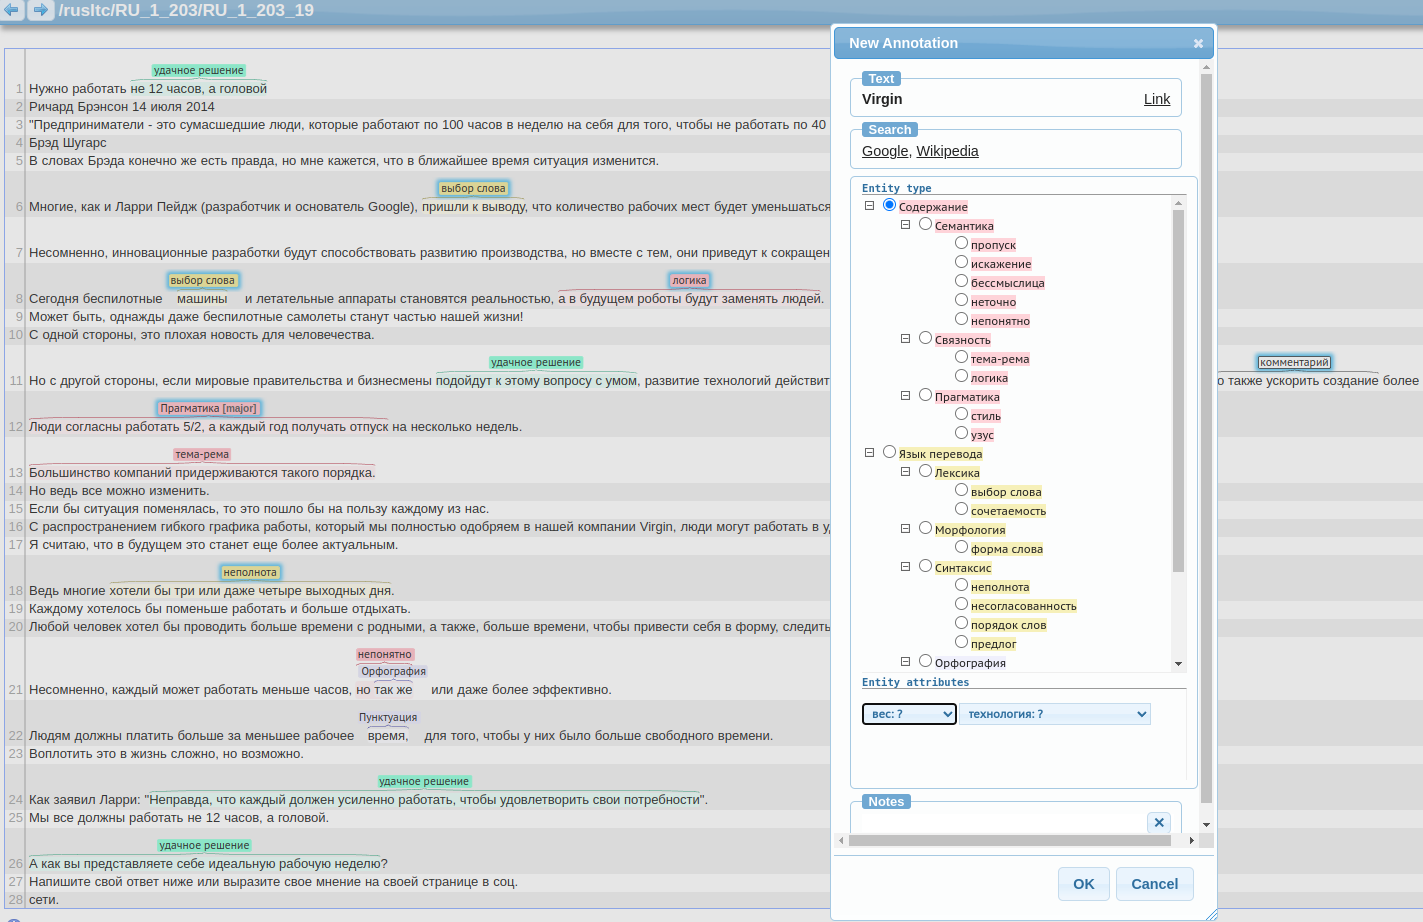
\includegraphics[width=\textwidth]{figures/brat}
\caption{\label{fig:brat}Screenshot of a \textit{brat}-based annotation environment}
\end{sidewaysfigure}

\begin{table}[H]
	\centering
	\begin{tabular}{lr}
		\toprule
		error type & weight \\
		\midrule
		Content               & 1   \\
		\hspace{1em}content\_reference    & 2   \\
		\hspace{3em}omission              & 2    \\
		\hspace{3em}distortion            & 3   \\
		\hspace{3em}nonsense              & 3   \\
		\hspace{3em}inexact               & 1   \\
		\hspace{3em}unclear               & 2   \\
		\hspace{1em}content\_cohesion     & 2   \\
		\hspace{3em}theme-rheme           & 1   \\
		\hspace{3em}logic                 & 3   \\
		\hspace{1em}content\_pragmatics   & 1   \\
		\hspace{3em}register              & 3   \\
		\hspace{3em}use                   & 2   \\
		\midrule
		Language              			  & 1    \\
		\hspace{1em}language\_lexical     & 1   \\
		\hspace{3em}choice-of-word        & 3  \\
		\hspace{3em}combinability         & 3  \\
		\hspace{1em}language\_morphology  & 1    \\
		\hspace{3em}wordform              & 1   \\
		\hspace{1em}language\_syntax      & 2   \\
		\hspace{3em}incomplete            & 3    \\
		\hspace{3em}ungrammatical         & 3   \\
		\hspace{3em}word\_order           & 2   \\
		\hspace{3em}preposition           & 3    \\
		\hspace{3em}delete                & 2   \\
		\hspace{1em}language\_spelling    & 1   \\
		\hspace{3em}capitals              & 1   \\
		\hspace{3em}typo                  & 1   \\
		\hspace{1em}language\_punctuation & 1   \\
		\bottomrule
	\end{tabular}
	\caption{\label{tab:errweights}Weights assigned to error categories for accuracy and fluency scores}
\end{table}

	\chapter{\label{appx:neural_res}Performance of neural classifiers}
%\addcontentsline{toc}{chapter}{Appendix C. Core MQM taxonomy}

\begin{table}[H]
	\centering
	\begin{tabular}{l|llll}
		\toprule
		representation & Accuracy        & Precision       & Recall          & F1              \\
		\midrule
		chance          & 47.72 (+/-5.93) & 47.72 (+/-5.93) & 47.70 (+/-6.00) & 47.58 (+/-5.95) \\
		\midrule
		UD              & 90.56 (+/-4.14) & 90.59 (+/-4.12) & 90.38 (+/-4.30) & 90.43 (+/-4.22) \\
		collgram        & 70.82 (+/-5.05) & 70.85 (+/-5.17) & 70.43 (+/-5.11) & 70.33 (+/-5.10) \\
		ngram           & 69.80 (+/-3.67) & 69.95 (+/-4.45) & 68.99 (+/-3.63) & 69.02 (+/-3.62) \\
		\textbf{all}             & 92.01 (+/-3.78) & 92.04 (+/-3.74) & 91.85 (+/-3.91) & \textbf{91.90} (+/-3.84) \\
		\midrule
		tfidf           & 95.34 (+/-2.04) & 95.31 (+/-2.10) & 95.34 (+/-2.05) & 95.29 (+/-2.05) \\
		\midrule
		stsb-xlm-r-m         & 93.01 (+/-1.50) & 93.04 (+/-1.53) & 92.91 (+/-1.51) & 92.93 (+/-1.51) \\
		TQmono-m       & 94.23 (+/-2.76) & 94.31 (+/-2.86) & 94.12 (+/-2.76) & 94.16 (+/-2.78) \\
		ruRoberta & 96.34 (+/-2.28) & 96.34 (+/-2.29) & 96.29 (+/-2.30) & 96.30 (+/-2.30) \\
		\textbf{mdeberta3}  & 96.45 (+/-1.84) & 96.47 (+/-1.77) & 96.40 (+/-1.93) & \boxit{0.4in} \textbf{96.41} (+/-1.87) \\
	\bottomrule
	\end{tabular}
	\caption{\label{tab:pro-ref_neu}Professional translations: results of translationese classification (neural classifier)}
\end{table}

\begin{table}[H]
	\centering
	\begin{tabular}{l|llll}
		\toprule
		representation & Accuracy        & Precision       & Recall          & F1              \\
		\midrule
		chance          & 50.05 (+/-3.72) & 48.65 (+/-3.80) & 48.62 (+/-3.88) & 48.59 (+/-3.84) \\
		\midrule
		UD              & 90.49 (+/-2.87) & 90.25 (+/-2.95) & 90.17 (+/-3.05) & 90.12 (+/-2.98) \\
		collgram        & 67.75 (+/-1.62) & 66.63 (+/-2.02) & 64.03 (+/-2.14) & 64.12 (+/-2.37) \\
		ngram           & 75.81 (+/-5.60) & 76.69 (+/-6.15) & 72.43 (+/-6.55) & 72.91 (+/-6.73) \\
		\textbf{all}             & 92.30 (+/-2.02) & 92.35 (+/-2.03) & 91.76 (+/-2.25) & \textbf{91.94} (+/-2.13) \\
		\midrule
		tfidf           & 94.11 (+/-2.49) & 93.64 (+/-2.57) & 94.68 (+/-2.39) & 93.96 (+/-2.54) \\
		\midrule
		stsb-xlm-r-m   & 89.54 (+/-3.34) & 89.41 (+/-3.15) & 89.00 (+/-3.66) & 89.06 (+/-3.52) \\
		TQmono-m & 95.79 (+/-2.02) & 95.69 (+/-2.05) & 95.65 (+/-2.16) & 95.63 (+/-2.10) \\
		ruRoberta & 97.59 (+/-1.78) & 97.50 (+/-1.83) & 97.55 (+/-1.91) & 97.50 (+/-1.86) \\
		\textbf{mdeberta3}  & 97.84 (+/-2.12) & 97.94 (+/-1.92) & 97.61 (+/-2.48) & \boxit{0.4in} \textbf{97.73} (+/-2.25) \\
	\bottomrule
	\end{tabular}
	\caption{\label{tab:stu-ref_neu}Student translations: results of translationese classification (neural classifier)}
\end{table}



\begin{table}[H]
	\centering
	\begin{tabular}{l|llll}
		\toprule
		representation & Accuracy        & Precision       & Recall          & F1              \\
		\midrule
		chance          & 49.59 (+/-3.47) & 49.45 (+/-3.48) & 49.45 (+/-3.51) & 49.39 (+/-3.49) \\
		\midrule
		UD              & 78.45 (+/-4.00) & 78.71 (+/-4.10) & 78.24 (+/-3.80) & 78.18 (+/-3.98) \\
		collgram        & 65.99 (+/-5.39) & 66.42 (+/-6.08) & 64.86 (+/-5.43) & 64.60 (+/-5.58) \\
		ngram           & 67.34 (+/-4.19) & 67.95 (+/-4.59) & 65.93 (+/-4.54) & 65.57 (+/-5.05) \\
		all             & 81.02 (+/-2.24) & 81.18 (+/-2.25) & 80.60 (+/-2.18) & 80.71 (+/-2.23) \\
		\midrule
		quest61         & 82.66 (+/-4.48) & 83.00 (+/-4.51) & 82.33 (+/-4.47) & 82.38 (+/-4.52) \\
%		quest17         & 78.44 (+/-4.63) & 79.07 (+/-4.63) & 78.21 (+/-4.67) & 78.07 (+/-4.67) \\
		\midrule
		tfidf           & 82.51 (+/-5.42) & 82.64 (+/-5.26) & 82.76 (+/-5.29) & 82.45 (+/-5.39) \\
		\midrule
		stsb-xlm-r-m          & 79.54 (+/-3.13) & 79.65 (+/-3.18) & 79.29 (+/-3.18) & 79.27 (+/-3.21) \\
		TQmono-m        & 84.55 (+/-4.46) & 84.81 (+/-4.44) & 84.10 (+/-4.60) & 84.26 (+/-4.58) \\
		ruRoberta & 89.43 (+/-2.68) & 89.65 (+/-2.70) & 89.18 (+/-2.75) & 89.28 (+/-2.74) \\
		\textbf{mdeberta3}  & 91.06 (+/-3.38) & 91.48 (+/-3.28) & 90.87 (+/-3.39) & \boxit{0.4in} \textbf{90.93} (+/-3.43) \\
	\bottomrule
	\end{tabular}
\caption{\label{tab:stu-pro_neu}Student vs Professional translations (neural classifier)}
\end{table}


\begin{table}[H]
	\centering
	\begin{tabular}{l|llll}
		\toprule
		representation & Accuracy         & Precision        & Recall           & F1               \\
		\midrule
		chance          & 51.67 (+/-7.78)  & 51.67 (+/-7.80)  & 51.67 (+/-7.78)  & 51.63 (+/-7.78)  \\
		\midrule
		\textbf{UD}              & 56.94 (+/-7.98)  & 57.08 (+/-7.95)  & 57.01 (+/-7.91)  & \textbf{56.74} (+/-8.07)  \\
		collgram        & 52.22 (+/-10.45) & 52.45 (+/-10.6) & 52.30 (+/-10.43) & 52.03 (+/-10.4) \\
		ngram           & 49.17 (+/-9.13)  & 49.32 (+/-9.66)  & 49.19 (+/-9.33)  & 48.66 (+/-9.17)  \\
		all             & 53.89 (+/-8.98)  & 53.92 (+/-9.15)  & 53.86 (+/-8.98)  & 53.60 (+/-9.06)  \\
		\midrule
		quest61 		& 47.22 (+/-8.43) & 47.29 (+/-8.78) & 47.15 (+/-8.48) & 46.88 (+/-8.26)  \\
		quest17         & 52.50 (+/-8.65)  & 52.59 (+/-8.76)  & 52.55 (+/-8.68)  & 52.19 (+/-8.72)  \\
		\midrule
		tfidf           & 56.39 (+/-6.70)  & 56.93 (+/-7.12)  & 56.52 (+/-6.77)  & 55.76 (+/-6.91)  \\
		\midrule
		stsb-xlm-r-m          & 49.17 (+/-7.86)  & 49.09 (+/-8.10)  & 49.21 (+/-7.91)  & 48.77 (+/-8.09)  \\
		TQmono-m        & 62.50 (+/-4.69)  & 63.20 (+/-4.40)  & 62.72 (+/-4.35)  & 62.11 (+/-5.05)  \\
		ruRoberta & 72.22 (+/-7.95)  & 72.55 (+/-7.79)  & 72.33 (+/-7.86)  & 72.14 (+/-8.01)  \\
		\textbf{mdeberta3}  & 79.44 (+/-6.83)  & 79.91 (+/-6.52)  & 79.49 (+/-6.84)  & \boxit{0.4in} \textbf{79.32} (+/-6.97) \\
		\bottomrule
	\end{tabular}
\caption{\label{tab:bad-good_neu}Bad vs Good: Binary quality classification (neural classifier)}
\end{table}


	\chapter{\label{appx:feat_analysis}Comparative-contrastive UD features}
%\addcontentsline{toc}{chapter}{Appendix C. Core MQM taxonomy}

Note: In Tables~\ref{tab:pro_indicators} and \ref{tab:stu_indicators} equals sign indicates no statistical differences; * marks cases where there are statistical differences between SL and TL (ref=src)

\begin{longtable}{l|p{2cm}p{2cm}p{1.5cm}ccc}
	\caption{\label{tab:pro_indicators}Properties of UD features sorted by degree of association between values in professional translations and non-translation}\\
	\toprule
	feature       & shapiro-tgt & shapiro-ref & bartlett & LogR & trend          & means \\
	\midrule
	acl           & -- & --   & --  & 0.62    & shining        & ref\textless{}src=tgt \\
	acl:relcl     & -- & --   & --  & 0.69    & overuse of SL & ref\textless{}tgt\textless{}src \\
	addit         & -- & --  & --   & 0.4     & shining   & ref\textless{}src=tgt \\
	adp           & -- & normal& --& 0.4  & useless   & tgt=ref=src   \\
	advcl         & -- & --   & --  & 0.7 & overuse of SL  & ref\textless{}tgt\textless{}src \\
	advers        & -- & --  & --   & 0.39 & overuse of SL  & ref\textless{}tgt\textless{}src \\
	advmod        & normal       & --  & equal& 0.53 & overuse of SL  & ref\textless{}tgt\textless{}src \\
	amod          & -- & --  & -- & 0.51    & russification  & src\textless{}ref\textless{}tgt \\
	anysome       & -- & --  & -- & 0.36    & overuse of SL  & ref\textless{}tgt\textless{}src \\
	appos         & -- & --  & -- & 0.39    & SL/TL-indep    & tgt\textless{}ref=src           \\
	attrib        & -- & --  & -- & 0.51    & russification  & src\textless{}ref\textless{}tgt \\
	aux           & -- & --  & -- & 0.42    & overuse of SL  & ref\textless{}tgt\textless{}src \\
	aux:pass      & -- & --  & equal & 0.36 & underuse of TL  & tgt\textless{}ref\textless{}src \\
	case          & -- & -- & -- & 0.54    & overuse of SL  & ref\textless{}tgt\textless{}src \\
	caus          & -- & -- & equal & 0.36    & russification  & src\textless{}ref\textless{}tgt \\
	ccomp         & -- & -- & -- & 0.63    & overuse of SL  & ref\textless{}tgt\textless{}src \\
	cconj         & -- & -- & -- & 0.36    & adaptation     & tgt=ref\textless{}src           \\
	compar        & -- & -- & -- & 0.38    & overuse of SL  & ref\textless{}tgt\textless{}src \\
	compound      & -- & -- & equal & 0.63    & adaptation     & tgt=ref\textless{}src           \\
	conj          & -- & --& -- & 0.37    & SL/TL-indep    & ref\textless{}tgt=src*          \\
	content-TTR  & -- & -- & -- & 0.36    & adaptation     & src\textless{}ref=tgt        \\
	content-dens & -- & -- & equal& 0.36    & normalisation  & src\textless{}tgt\textless{}ref \\
	copula        & -- & -- & --& 0.52 & overuse of SL  & ref\textless{}tgt\textless{}src \\
	determ        & normal       & -- & equal & 0.36    & overuse of SL  & ref\textless{}tgt\textless{}src \\
	deverbals     & -- & -- & -- & 0.45 & normalisation  & src\textless{}tgt\textless{}ref \\
	discourse     & -- & -- & equal & 0.63    & useless  & tgt=ref=src                     \\
	epist         & -- & -- & -- & 0.45 & anglicisation  & ref\textless{}src\textless{}tgt \\
	finites       & normal       & -- & -- & 0.45 & adaptation     & tgt=ref\textless{}src           \\
	fixed         & -- & -- & --       & 0.56    & russification  & src\textless{}ref\textless{}tgt \\
	flat          & -- & -- & equal    & 0.36    & underuse of TL  & tgt\textless{}ref\textless{}src \\
	infs          & -- & -- & equal    & 0.39    & russification  & src\textless{}ref\textless{}tgt \\
	interrog      & -- & -- & --       & 0.39    & shining        & ref\textless{}tgt=src           \\
	iobj          & -- & -- & --       & 0.58    & russification  & src\textless{}ref\textless{}tgt \\
	mark          & -- & -- & --       & 0.74    & overuse of SL  & ref\textless{}tgt\textless{}src \\
	mdd           & normal       & -- & --       & 0.57    & overuse of SL  & ref\textless{}tgt\textless{}src \\
	mhd           & -- & -- & equal    & 0.63    & SL/TL-indep    & ref=src\textless{}tgt           \\
	mpred         & -- & -- & equal    & 0.53    & overuse of SL  & ref\textless{}tgt\textless{}src \\
	mquantif      & -- & -- & equal    & 0.36    & shining        & ref\textless{}src=tgt           \\
	neg           & -- & -- & --       & 0.41    & normalisation  & src\textless{}tgt\textless{}ref \\
	nmod          & -- & -- & equal    & 0.74    & adaptation     & src\textless{}ref=tgt        \\
	nn            & normal       & -- & equal    & 0.38    & normalisation  & src\textless{}tgt\textless{}ref \\
	nnargs        & -- & -- & --       & 0.68    & normalisation  & src\textless{}tgt\textless{}ref \\
	nsubj         & -- & -- & --       & 0.82    & overuse of SL  & ref\textless{}tgt\textless{}src \\
	numcls        & -- & normal       & --       & 0.71    & anglicisation  & ref\textless{}src\textless{}tgt \\
	nummod        & -- & -- & --       & 0.46    & normalisation        & src=tgt\textless{}ref           \\
	obj           & -- & -- & --       & 0.72    & overuse of SL  & ref\textless{}tgt\textless{}src \\
	obl           & -- & -- & --       & 0.64    & russification  & src\textless{}ref\textless{}tgt \\
	parataxis     & -- & -- & equal    & 0.64    & adaptation     & src\textless{}ref=tgt        \\
	passives      & -- & -- & --       & 0.36    & normalisation  & src\textless{}tgt\textless{}ref \\
	pasttense     & -- & -- & --       & 0.51    & SL/TL-indep    & tgt\textless{}ref=src           \\
	possp         & -- & -- & --       & 0.36    & russification  & src\textless{}ref\textless{}tgt \\
	ppron         & -- & -- & --       & 0.36    & overuse of SL  & ref\textless{}tgt\textless{}src \\
	pverbals      & -- & -- & --       & 0.36    & adaptation     & src\textless{}ref=tgt        \\
	sconj         & -- & -- & --       & 0.36    & russification  & src\textless{}ref\textless{}tgt \\
	sentlength    & -- & -- & --       & 0.61    & NA  & ref\textless{}tgt \\
	simple        & -- & -- & equal    & 0.67    & underuse of TL & tgt\textless{}src\textless{}ref \\
	superl        & -- & -- & equal    & 0.67    & adaptation     & tgt=ref\textless{}src           \\
	tempseq       & -- & -- & --       & 0.67    & adaptation     & tgt=ref\textless{}src           \\
	wdlength      & -- & normal       & --       & 0.4     & NA  & tgt\textless{}ref \\
	xcomp         & -- & -- & --       & 0.68    & shining        & ref\textless{}src=tgt
		
%		\bottomrule
\end{longtable}


\begin{longtable}{l|p{2cm}p{2cm}p{1.5cm}ccc}
	\caption{\label{tab:stu_indicators}Properties of UD features sorted by degree of association between values in student translations and non-translations}\\
	\toprule
	feature       & shapiro-tgt & shapiro-ref & bartlett & LogR-F1 & trend          & means \\
	\midrule
	acl           & --     & --     & --    & 0.56 & shining        & ref\textless{}src=tgt           \\
	acl:relcl     & --     & --     & --    & 0.66 & overuse of SL  & ref\textless{}tgt\textless{}src \\
	addit         & --     & --     & --    & 0.43 & SL/TL-indep    & ref=src\textless{}tgt           \\
	adp           & --     & normal & --    & 0.43 & adaptation     & tgt=ref\textless{}src           \\
	advcl         & --     & --     & --    & 0.63 & overuse of SL  & ref\textless{}tgt\textless{}src \\
	advers        & --     & --     & --    & 0.43 & adaptation     & tgt=ref\textless{}src           \\
	advmod        & --     & --     & --    & 0.38 & SL/TL-indep    & tgt\textless{}ref=src           \\
	amod          & --     & --     & --    & 0.53 & russification  & src\textless{}ref\textless{}tgt \\
	anysome       & --     & --     & --    & 0.43 & adaptation     & tgt=ref\textless{}src           \\
	appos         & --     & --     & equal & 0.37 & underuse of TL & tgt=src\textless{}ref           \\
	attrib        & --     & --     & --    & 0.52 & russification  & src\textless{}ref\textless{}tgt \\
	aux           & --     & --     & --    & 0.37 & adaptation     & tgt=ref\textless{}src           \\
	aux:pass      & --     & --     & --    & 0.37 & adaptation     & tgt=ref\textless{}src           \\
	case          & --     & --     & --    & 0.54 & overuse of SL  & ref\textless{}tgt\textless{}src \\
	caus          & --     & --     & --    & 0.37 & normalisation  & src\textless{}tgt\textless{}ref \\
	ccomp         & --     & --     & --    & 0.50 & overuse of SL  & ref\textless{}tgt\textless{}src \\
	cconj         & --     & --     & --    & 0.37 & adaptation     & tgt=ref\textless{}src           \\
	compar        & --     & --     & --    & 0.38 & overuse of SL  & ref\textless{}tgt\textless{}src \\
	compound      & --     & --     & --    & 0.37 & underuse of TL  & tgt\textless{}ref\textless{}src \\
	conj          & --     & --     & --    & 0.46 & SL/TL-indep    & ref=src\textless{}tgt           \\
	content\_TTR  & --     & --     & --    & 0.37 & underuse of TL & tgt\textless{}src\textless{}ref \\
	content\_dens & normal & --     & --    & 0.37 & russification  & src\textless{}ref\textless{}tgt \\
	copula        & --     & --     & --    & 0.51 & overuse of SL  & ref\textless{}tgt\textless{}src \\
	determ        & --     & --     & --    & 0.37 & overuse of SL  & ref\textless{}tgt\textless{}src \\
	deverbals     & --     & --     & --    & 0.45 & russification  & src\textless{}ref\textless{}tgt \\
	discourse     & --     & --     & --    & 0.37 & underuse of TL & tgt=src\textless{}ref           \\
	epist         & --     & --     & --    & 0.45 & adaptation     & tgt=ref\textless{}src           \\
	finites       & --     & --     & --    & 0.38 & overuse of SL  & ref\textless{}tgt\textless{}src \\
	fixed         & --     & --     & --    & 0.58 & russification  & src\textless{}ref\textless{}tgt \\
	flat          & --     & --     & --    & 0.37 & underuse of TL  & tgt\textless{}ref\textless{}src \\
	infs          & --     & --     & --    & 0.38 & adaptation     & src\textless{}ref=tgt        \\
	interrog      & --     & --     & --    & 0.38 & useless        & tgt=ref=src                     \\
	iobj          & --     & --     & --    & 0.37 & normalisation  & src\textless{}tgt\textless{}ref \\
	mark          & --     & --     & --    & 0.68 & overuse of SL  & ref\textless{}tgt\textless{}src \\
	mdd           & --     & --     & --    & 0.39 & overuse of SL  & ref\textless{}tgt\textless{}src \\
	mhd           & --     & --     & --    & 0.63 & SL/TL-indep    & ref=src\textless{}tgt           \\
	mpred         & --     & --     & --    & 0.44 & overuse of SL  & ref\textless{}tgt\textless{}src \\
	mquantif      & --     & --     & --    & 0.44 & useless        & tgt=ref=src                     \\
	neg           & --     & --     & --    & 0.40 & normalisation  & src\textless{}tgt\textless{}ref \\
	nmod          & --     & --     & --    & 0.50 & russification  & src\textless{}ref\textless{}tgt \\
	nn            & --     & --     & --    & 0.37 & russification  & src\textless{}ref\textless{}tgt \\
	nnargs        & --     & --     & --    & 0.55 & normalisation  & src\textless{}tgt\textless{}ref \\
	nsubj         & --     & --     & --    & 0.71 & shining        & ref\textless{}tgt=src           \\
	numcls        & --     & normal & --    & 0.52 & russification  & src\textless{}ref\textless{}tgt \\
	nummod        & --     & --     & --    & 0.71 & adaptation     & src\textless{}ref=tgt        \\
	obj           & --     & --     & --    & 0.61 & overuse of SL  & ref\textless{}tgt\textless{}src \\
	obl           & --     & --     & --    & 0.59 & russification  & src\textless{}ref\textless{}tgt \\
	parataxis     & --     & --     & equal & 0.67 & normalisation  & src\textless{}tgt\textless{}ref \\
	passives      & --     & --     & equal & 0.37 & normalisation  & src\textless{}tgt\textless{}ref \\
	pasttense     & --     & --     & equal & 0.42 & SL/TL-indep    & tgt\textless{}ref=src           \\
	possp         & --     & --     & --    & 0.42 & adaptation     & src\textless{}ref=tgt        \\
	ppron         & --     & --     & --    & 0.37 & overuse of SL  & ref\textless{}tgt\textless{}src \\
	pverbals      & --     & --     & equal & 0.37 & adaptation     & src\textless{}ref=tgt        \\  % src<ref=tgt
	sconj         & normal & --     & --    & 0.37 & russification  & src\textless{}ref\textless{}tgt \\
	sentlength    & --     & --     & --    & 0.57 & NA  & ref\textless{}tgt \\
	simple        & --     & --     & --    & 0.37 & underuse of TL  & tgt\textless{}ref\textless{}src \\
	superl        & --     & --     & --    & 0.37 & adaptation     & tgt=ref\textless{}src           \\
	tempseq       & --     & --     & --    & 0.37 & adaptation     & tgt=ref\textless{}src           \\
	wdlength      & normal & normal & --    & 0.43 & NA  & ref\textless{}tgt \\
	xcomp         & --     & --     & --    & 0.52 & shining        & ref\textless{}src=tgt			\\
	\bottomrule

\end{longtable}


\end{appendices}

\end{document}